% Options for packages loaded elsewhere
\PassOptionsToPackage{unicode}{hyperref}
\PassOptionsToPackage{hyphens}{url}
%
\documentclass[
  oneside]{book}
\usepackage{amsmath,amssymb}
\usepackage{lmodern}
\usepackage{ifxetex,ifluatex}
\ifnum 0\ifxetex 1\fi\ifluatex 1\fi=0 % if pdftex
  \usepackage[T1]{fontenc}
  \usepackage[utf8]{inputenc}
  \usepackage{textcomp} % provide euro and other symbols
\else % if luatex or xetex
  \usepackage{unicode-math}
  \defaultfontfeatures{Scale=MatchLowercase}
  \defaultfontfeatures[\rmfamily]{Ligatures=TeX,Scale=1}
\fi
% Use upquote if available, for straight quotes in verbatim environments
\IfFileExists{upquote.sty}{\usepackage{upquote}}{}
\IfFileExists{microtype.sty}{% use microtype if available
  \usepackage[]{microtype}
  \UseMicrotypeSet[protrusion]{basicmath} % disable protrusion for tt fonts
}{}
\makeatletter
\@ifundefined{KOMAClassName}{% if non-KOMA class
  \IfFileExists{parskip.sty}{%
    \usepackage{parskip}
  }{% else
    \setlength{\parindent}{0pt}
    \setlength{\parskip}{6pt plus 2pt minus 1pt}}
}{% if KOMA class
  \KOMAoptions{parskip=half}}
\makeatother
\usepackage{xcolor}
\IfFileExists{xurl.sty}{\usepackage{xurl}}{} % add URL line breaks if available
\IfFileExists{bookmark.sty}{\usepackage{bookmark}}{\usepackage{hyperref}}
\hypersetup{
  pdftitle={Create a cryptocurrency trading bot in Elixir},
  pdfauthor={Kamil Skowron},
  hidelinks,
  pdfcreator={LaTeX via pandoc}}
\urlstyle{same} % disable monospaced font for URLs
\usepackage[left=3cm, right=3cm, top=2.5cm, bottom=2.5cm]{geometry}
\usepackage{color}
\usepackage{fancyvrb}
\newcommand{\VerbBar}{|}
\newcommand{\VERB}{\Verb[commandchars=\\\{\}]}
\DefineVerbatimEnvironment{Highlighting}{Verbatim}{commandchars=\\\{\}}
% Add ',fontsize=\small' for more characters per line
\usepackage{framed}
\definecolor{shadecolor}{RGB}{248,248,248}
\newenvironment{Shaded}{\begin{snugshade}}{\end{snugshade}}
\newcommand{\AlertTok}[1]{\textcolor[rgb]{0.94,0.16,0.16}{#1}}
\newcommand{\AnnotationTok}[1]{\textcolor[rgb]{0.56,0.35,0.01}{\textbf{\textit{#1}}}}
\newcommand{\AttributeTok}[1]{\textcolor[rgb]{0.77,0.63,0.00}{#1}}
\newcommand{\BaseNTok}[1]{\textcolor[rgb]{0.00,0.00,0.81}{#1}}
\newcommand{\BuiltInTok}[1]{#1}
\newcommand{\CharTok}[1]{\textcolor[rgb]{0.31,0.60,0.02}{#1}}
\newcommand{\CommentTok}[1]{\textcolor[rgb]{0.56,0.35,0.01}{\textit{#1}}}
\newcommand{\CommentVarTok}[1]{\textcolor[rgb]{0.56,0.35,0.01}{\textbf{\textit{#1}}}}
\newcommand{\ConstantTok}[1]{\textcolor[rgb]{0.00,0.00,0.00}{#1}}
\newcommand{\ControlFlowTok}[1]{\textcolor[rgb]{0.13,0.29,0.53}{\textbf{#1}}}
\newcommand{\DataTypeTok}[1]{\textcolor[rgb]{0.13,0.29,0.53}{#1}}
\newcommand{\DecValTok}[1]{\textcolor[rgb]{0.00,0.00,0.81}{#1}}
\newcommand{\DocumentationTok}[1]{\textcolor[rgb]{0.56,0.35,0.01}{\textbf{\textit{#1}}}}
\newcommand{\ErrorTok}[1]{\textcolor[rgb]{0.64,0.00,0.00}{\textbf{#1}}}
\newcommand{\ExtensionTok}[1]{#1}
\newcommand{\FloatTok}[1]{\textcolor[rgb]{0.00,0.00,0.81}{#1}}
\newcommand{\FunctionTok}[1]{\textcolor[rgb]{0.00,0.00,0.00}{#1}}
\newcommand{\ImportTok}[1]{#1}
\newcommand{\InformationTok}[1]{\textcolor[rgb]{0.56,0.35,0.01}{\textbf{\textit{#1}}}}
\newcommand{\KeywordTok}[1]{\textcolor[rgb]{0.13,0.29,0.53}{\textbf{#1}}}
\newcommand{\NormalTok}[1]{#1}
\newcommand{\OperatorTok}[1]{\textcolor[rgb]{0.81,0.36,0.00}{\textbf{#1}}}
\newcommand{\OtherTok}[1]{\textcolor[rgb]{0.56,0.35,0.01}{#1}}
\newcommand{\PreprocessorTok}[1]{\textcolor[rgb]{0.56,0.35,0.01}{\textit{#1}}}
\newcommand{\RegionMarkerTok}[1]{#1}
\newcommand{\SpecialCharTok}[1]{\textcolor[rgb]{0.00,0.00,0.00}{#1}}
\newcommand{\SpecialStringTok}[1]{\textcolor[rgb]{0.31,0.60,0.02}{#1}}
\newcommand{\StringTok}[1]{\textcolor[rgb]{0.31,0.60,0.02}{#1}}
\newcommand{\VariableTok}[1]{\textcolor[rgb]{0.00,0.00,0.00}{#1}}
\newcommand{\VerbatimStringTok}[1]{\textcolor[rgb]{0.31,0.60,0.02}{#1}}
\newcommand{\WarningTok}[1]{\textcolor[rgb]{0.56,0.35,0.01}{\textbf{\textit{#1}}}}
\usepackage{longtable,booktabs,array}
\usepackage{calc} % for calculating minipage widths
% Correct order of tables after \paragraph or \subparagraph
\usepackage{etoolbox}
\makeatletter
\patchcmd\longtable{\par}{\if@noskipsec\mbox{}\fi\par}{}{}
\makeatother
% Allow footnotes in longtable head/foot
\IfFileExists{footnotehyper.sty}{\usepackage{footnotehyper}}{\usepackage{footnote}}
\makesavenoteenv{longtable}
\usepackage{graphicx}
\makeatletter
\def\maxwidth{\ifdim\Gin@nat@width>\linewidth\linewidth\else\Gin@nat@width\fi}
\def\maxheight{\ifdim\Gin@nat@height>\textheight\textheight\else\Gin@nat@height\fi}
\makeatother
% Scale images if necessary, so that they will not overflow the page
% margins by default, and it is still possible to overwrite the defaults
% using explicit options in \includegraphics[width, height, ...]{}
\setkeys{Gin}{width=\maxwidth,height=\maxheight,keepaspectratio}
% Set default figure placement to htbp
\makeatletter
\def\fps@figure{htbp}
\makeatother
\setlength{\emergencystretch}{3em} % prevent overfull lines
\providecommand{\tightlist}{%
  \setlength{\itemsep}{0pt}\setlength{\parskip}{0pt}}
\setcounter{secnumdepth}{5}
% sample comment
\ifluatex
  \usepackage{selnolig}  % disable illegal ligatures
\fi
\usepackage[]{natbib}
\bibliographystyle{plainnat}

\title{Create a cryptocurrency trading bot in Elixir}
\author{Kamil Skowron}
\date{0.1.1}

\begin{document}
\maketitle

{
\setcounter{tocdepth}{1}
\tableofcontents
}
\hypertarget{welcome}{%
\chapter*{Welcome 👋}\label{welcome}}
\addcontentsline{toc}{chapter}{Welcome 👋}

This website is the home of \textbf{Create a cryptocurrency trading bot in Elixir} book.

\textbf{This book is 75\% complete} - chapters 1-15 are finished but I'm planning to add more content in the near future.

Are you looking for a real-world project to gain hands-on experience/solidify your understanding of Elixir/OTP? You are in the right place! We will venture on a journey to create a cryptocurrency trading bot in Elixir. You will be able to see first-hand, how complex systems are designed and developed as we will build them together!

This book is based on \href{https://www.youtube.com/watch?v=wVYIx7M6o28\&list=PLxsE19GnjC5Nv1CbeKOiS5YqGqw35aZFJ}{Create a cryptocurrency trading bot in Elixir} video series released on YouTube.

This work is licensed under the Creative Commons Attribution-NonCommercial-ShareAlike 4.0 International \href{https://creativecommons.org/licenses/by-nc-sa/4.0/}{CC BY-NC-SA 4.0}.

\textbf{To get notified about updates} to this book just ``watch'' the \href{https://github.com/frathon/create-a-cryptocurrency-trading-bot-in-elixir}{source code's repository} and don't forget to leave a ⭐:

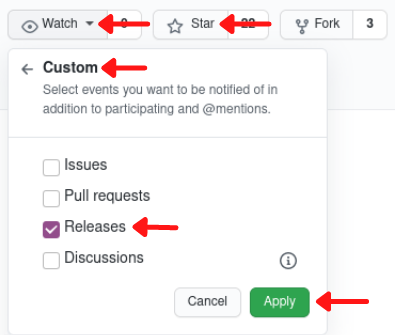
\includegraphics{images/watch_book_howto.png}

\hypertarget{limit-of-liabilitydisclaimer-of-warranty}{%
\section*{Limit of Liability/Disclaimer of Warranty}\label{limit-of-liabilitydisclaimer-of-warranty}}
\addcontentsline{toc}{section}{Limit of Liability/Disclaimer of Warranty}

\textbf{THIS BOOK IS NOT A FINANCIAL ADVICE}

THE SOFTWARE/BOOK IS PROVIDED ``AS IS'', WITHOUT WARRANTY OF ANY KIND, EXPRESS OR IMPLIED, INCLUDING BUT NOT LIMITED TO THE WARRANTIES OF MERCHANTABILITY, FITNESS FOR A PARTICULAR PURPOSE AND NONINFRINGEMENT. IN NO EVENT SHALL THE AUTHORS OR COPYRIGHT HOLDERS BE LIABLE FOR ANY CLAIM, DAMAGES OR OTHER LIABILITY, WHETHER IN AN ACTION OF CONTRACT, TORT OR OTHERWISE, ARISING FROM, OUT OF OR IN CONNECTION WITH THE SOFTWARE/BOOK OR THE USE OR OTHER DEALINGS IN THE SOFTWARE/BOOK.

\hypertarget{contributing-errata}{%
\section*{Contributing / Errata}\label{contributing-errata}}
\addcontentsline{toc}{section}{Contributing / Errata}

The book is written using \href{http://rmarkdown.rstudio.com/}{R Markdown}(it's a very similar syntax to the GitHub markdown but supports many more features including code execution, etc.) and converted to final form (for example PDF) using the \href{https://www.bookdown.org/}{bookdown} app. This means that editing a chapter is as simple as editing the markdown for that chapter - there is even an edit button at the top of the page to do exactly that. I would love to follow the standard process of forking, making changes, opening PR, merging, and releasing a new version of the book. I invite people to open issues as well with suggestions.

\hypertarget{backers}{%
\section*{Backers}\label{backers}}
\addcontentsline{toc}{section}{Backers}

This book was initially published via Leanpub, but to keep it up to date as well as publicly available for people that can't afford to pay for it, it's now available here free of charge.

Knowledge is power and should be shared equally 🙏

\textbf{Please consider supporting this book and my other work via the} \href{https://github.com/sponsors/frathon}{\textbf{GitHub Sponsors}} \textbf{program}(it supports both one-off payments as well as ``monthly'' plans).

\hypertarget{preface}{%
\section*{Preface}\label{preface}}
\addcontentsline{toc}{section}{Preface}

In recent years \href{https://elixir-lang.org/}{Elixir} programming language gained a lot of interest in the industry.

Its unmatched parallelization capabilities are unique and powerful, making it a great candidate for highly concurrent systems like the ones trading assets on exchanges.

In this book, we will go through the development process of a cryptocurrency trading bot in Elixir. We will start grounds up and chapter by chapter progress with the implementation ending up with a fully fledged \emph{naive} trading strategy. We will be designing process supervision trees, describing why specific decisions were taken and how will they impact the system going forward.

By any stretch of the imagination, I don't believe that ``this is \emph{the only} way''(nor even the best way) to create a cryptocurrency trading bot in Elixir. This book focuses more on building a real-life project and iterating over it, taking decisions on the way as it would happen in a real work environment. There are parts that will be ``perfect'' the first time around, but there are also others, where we will take compromises to ``get it to working'' and then when the time is right, we will refactor them as we will gain a better understanding of the domain problem.

\hypertarget{who-this-book-is-for}{%
\section*{Who this book is for}\label{who-this-book-is-for}}
\addcontentsline{toc}{section}{Who this book is for}

This book will be a great resource for everyone that already knows the basics of Elixir and wants to get a feel of how developing a non-trivial system looks like using it.

Readers do not need deep knowledge about cryptocurrencies to follow along as I will shy away from crypto / trading jargon as well as will explain it whenever it's unavoidable.

\textbf{This is not a book focused on trading strategies, neither it's financial advice to trade at all.} The main focus of this book is to showcase how the implementation of even complex problems can be achieved in Elixir by simple processes working together in a orchestrated manner.

\textbf{The strategy described in this book is naive and most probably will end up losing money}, but that's not the point of this book. \textbf{As we will build up the strategy we will face a spectrum of problems that developers face at work. It's a great primer if you want to get your first ``project'' behind your belt}.

So, if you've already gone through the motions and learned Elixir and OTP but still feel like you need to get your hands dirty with a ``real problem'' to ``make it stick'', this book is for you.

\hypertarget{what-this-book-covers}{%
\section*{What this book covers}\label{what-this-book-covers}}
\addcontentsline{toc}{section}{What this book covers}

This book is a loosely written representation of ``\href{https://www.youtube.com/watch?v=wVYIx7M6o28\&list=PLxsE19GnjC5Nv1CbeKOiS5YqGqw35aZFJ}{Create a cryptocurrency trading bot in Elixir}'' video course released on YouTube.

It's still an ongoing production and will be continued in the upcoming months, at this moment it contains:

\begin{itemize}
\tightlist
\item
  Chapter 1 - Stream live crypto prices from Binance WSS
\end{itemize}

Stream live cryptocurrency prices (trade events) from the Binance exchange. Starting grounds up, we will create a new umbrella project and a \texttt{streamer} application inside it. The streamer application will use a Websocket client called \texttt{WebSockex} to establish a connection with the Binance API and receive a live feed. After receiving the event as JSON string, we will decode it using the \texttt{jason} library and convert it to our own data struct. At the end of the chapter, we will see decoded trade events being logged to the terminal.

\begin{itemize}
\tightlist
\item
  Chapter 2 - Create a naive trading strategy - single trader without supervision
\end{itemize}

In this chapter we will create our first \emph{naive} trading strategy. We will create another application inside our umbrella called \texttt{naive}. We will put data streamed to our \texttt{streamer} application to good use by sending it over to the \texttt{naive} application. We will start with a very basic solution consisting of single process called \texttt{trader} that will utilize the \texttt{GenServer} behaviour. It will allow us to go through the full trading cycle and will give us something that ``works''.

\begin{itemize}
\tightlist
\item
  Chapter 3 - Introduce PubSub as a communication method
\end{itemize}

To allow our trading strategy to scale to multiple parallel traders, we need to find a way to distribute the latest prices (trade events) to those multiple traders. We will introduce PubSub to broadcast messages from the streamer(s) to the trader(s). PubSub will allow us to break hardcoded references between applications in our umbrella and that will become a pattern that we will utilize moving forward.

\begin{itemize}
\tightlist
\item
  Chapter 4 - Mock the Binance API
\end{itemize}

Besides historical prices (trade events), to perform backtesting, we need to be able to mock placing orders and get trade events back as they are filled. In this chapter we will focus on developing the solution that will allow our trader to ``trade'' without contacting the Binance exchange(for people without Binance accounts), it will also allow us to backtest our trading strategy.

\begin{itemize}
\tightlist
\item
  Chapter 5 - Enable parallel trading on multiple symbols
\end{itemize}

Our basic strategy implementation from the last chapter is definitely too basic to be used in a ``production environment'' - it can't be neither scaled nor it is fault-tolerant. In this chapter, we will upgrade our naive strategy to be more resilient. This will require a supervision tree to be created and will allow us to see different supervision strategies in action and understand the motivation behind using and stacking them.

\begin{itemize}
\tightlist
\item
  Chapter 6 - Introduce a \texttt{buy\_down\_interval} to make a single trader more profitable
\end{itemize}

At this moment our \texttt{Naive.Trader} implementation will blindly place a buy order at the price of the last trade event. Whenever the \texttt{Naive.Trader} process will finish trade, a new \texttt{Naive.Trader} process will be started and it will end up placing a buy order at the same price as the price of the previous sell order. This will cost us double the fee without gaining any advantage and would cause further complications down the line so we will introduce a \texttt{buy\_down\_interval} which will allow the \texttt{Naive.Trader} processes to place buy order below the current trade event's price.

\begin{itemize}
\tightlist
\item
  Chapter 7 - Introduce a trader budget and calculating the quantity
\end{itemize}

Since the second chapter our \texttt{Naive.Trader} processes are placing orders with a hardcoded quantity of 100. In this chapter, we will introduce a budget that will be evenly split between the \texttt{Naive.Trader} processes using chunks. We will utilize that budget to calculate quantity (to be able to do that we need to fetch further \texttt{step\_size} information from the Binance API)

\begin{itemize}
\tightlist
\item
  Chapter 8 - Add support for multiple transactions per order
\end{itemize}

Our \texttt{Naive.Trader} implementation assumes that our orders will be filled within a single transaction, but this isn't always the case. In this chapter, we will discuss how could we implement the support for multiple transactions per order and race conditions that could occur between the bot and the Binance API.

\begin{itemize}
\tightlist
\item
  Chapter 9 - Run multiple traders in parallel
\end{itemize}

With PubSub, supervision tree, buy down and budget in place we can progress with scaling the number of traders. This will require further improvements to our trading strategy like introducing a \texttt{rebuy\_interval}. At the end of this chapter our trading strategy will be able to start and run multiple traders in parallel.

\begin{itemize}
\tightlist
\item
  Chapter 10 - Fine-tune trading strategy per symbol
\end{itemize}

Currently naive strategy works based on settings hardcoded in the \texttt{leader} module. To allow for fine-tunning the naive trading strategy per symbol we will introduce a new database together with table that will store trading settings.

\begin{itemize}
\tightlist
\item
  Chapter 11 - Supervise and autostart streaming
\end{itemize}

In the last chapter we introduced a new database inside the \texttt{naive} application to store default settings, in this chapter we will do the same for the \texttt{streamer} application. Inside the settings there will be a \texttt{status} flag that will allow us to implement the autostarting functionality on initialization using Task abstracting

\begin{itemize}
\tightlist
\item
  Chapter 12 - Start, stop, shutdown and autostart trading
\end{itemize}

To follow up after autostarting streaming we will apply the same trick to the trading supervision tree using Task abstraction. We will need to introduce new supervision level to achieve correct supervision strategy.

\begin{itemize}
\tightlist
\item
  Chapter 13 - Abstract duplicated supervision code
\end{itemize}

As both the \texttt{naive} and the \texttt{streamer} application contain almost the same copy-pasted code that allows us to start, stop and autostart workers. We will look into how could we abstract the common parts of that implementation to a single module. We will venture into utilizing the \texttt{\_\_using\_\_} macro to get rid of the boilerplate.

\begin{itemize}
\tightlist
\item
  Chapter 14 - Store trade events and orders inside the database
\end{itemize}

To be able to backtest the trading strategy, we need to have historical prices (trade events) and list of orders that were placed stored in the database, which will be the focus of this chapter. At this moment, the latest prices (trade events) are broadcasted to PubSub topic and traders are subscribing to it. We will create a new application called \texttt{data\_warehouse} inside our umbrella that will be responsible for subscribing to the same PubSub topics and storing incoming prices (trade events) in the Postgres database. We will update the \texttt{Naive.Trader} module to broadcast orders as traders will place them.

Then we will move on to adding supervision similar to the one from the \texttt{naive} and the \texttt{streamer} applications but this time we will show how we could avoid using both common module and macros by utilizing the \texttt{Registry} module.

\begin{itemize}
\tightlist
\item
  Chapter 15 - Backtest trading strategy
\end{itemize}

In this chapter, we will be backtesting our trading strategy by developing a publisher inside the DataWarehouse application. It will stream trade events from the database to broadcast them to the \texttt{TRADE\_EVENTS:\#\{symbol\}} PubSub topic. It will use the same topic as data would be streamed directly from the Binance. From the trader's perspective, it won't any difference and will cause normal trading activity that will be stored inside the database to be analyzed later.

\hypertarget{source-code}{%
\section*{Source code}\label{source-code}}
\addcontentsline{toc}{section}{Source code}

The source code for this book is hosted on Github:

\url{https://github.com/frathon/create-a-cryptocurrency-trading-bot-in-elixir-source-code}

Final code of each chapter has it's own branch.

\hypertarget{stream-live-crypto-prices-from-binance-wss}{%
\chapter{Stream live crypto prices from Binance WSS}\label{stream-live-crypto-prices-from-binance-wss}}

\hypertarget{objectives}{%
\section{Objectives}\label{objectives}}

\begin{itemize}
\tightlist
\item
  create an umbrella app
\item
  create a supervised application inside an umbrella
\item
  connect to Binance's WebSocket Stream using the WebSockex module
\item
  define a TradeEvent struct that will hold incoming data
\item
  decode incoming events using the Jason module
\end{itemize}

\hypertarget{create-an-umbrella-app}{%
\section{Create an umbrella app}\label{create-an-umbrella-app}}

In the beginning, there was nothing\ldots{} so we need to create an umbrella project:

\begin{Shaded}
\begin{Highlighting}[]
\ExtensionTok{mix}\NormalTok{ new hedgehog }\AttributeTok{{-}{-}umbrella}
\end{Highlighting}
\end{Shaded}

\hypertarget{create-a-supervised-application-inside-an-umbrella}{%
\section{Create a supervised application inside an umbrella}\label{create-a-supervised-application-inside-an-umbrella}}

We can now proceed with creating a new supervised application called \texttt{streamer} inside our umbrella:

\begin{Shaded}
\begin{Highlighting}[]
\BuiltInTok{cd}\NormalTok{ hedgehog/apps}
\ExtensionTok{mix}\NormalTok{ new streamer }\AttributeTok{{-}{-}sup}
\end{Highlighting}
\end{Shaded}

\hypertarget{connect-to-binances-websocket-stream-using-the-websockex-module}{%
\section{Connect to Binance's WebSocket Stream using the WebSockex module}\label{connect-to-binances-websocket-stream-using-the-websockex-module}}

To establish a connection to Binance API's stream, we will need to use a WebSocket client. The module that we will use is called \href{https://github.com/Azolo/websockex}{WebSockex}. Scrolling down to the \texttt{Installation} section inside module's readme on Github, we are instructed what dependency we need to add to our project.

We will append \texttt{:websockex} to the \texttt{deps} function inside the \texttt{mix.exs} file of the \texttt{streamer} application:

\begin{Shaded}
\begin{Highlighting}[]
  \CommentTok{\# /apps/streamer/mix.exs}
  \KeywordTok{defp}\NormalTok{ deps }\KeywordTok{do}
\NormalTok{    [}
\NormalTok{      \{}\VariableTok{:websockex}\NormalTok{, }\StringTok{"\textasciitilde{}\textgreater{} 0.4.2"}\NormalTok{\}}
\NormalTok{    ]}
  \KeywordTok{end}
\end{Highlighting}
\end{Shaded}

As we added a dependency to our project, we need to fetch it using \texttt{mix\ deps.get}.

We can now progress with creating a module that will be responsible for streaming. We will create a new file called \texttt{binance.ex} inside the \texttt{apps/streamer/lib/streamer} directory.

From the readme of \href{https://github.com/Azolo/websockex}{WebSockex} module, we can see that to use it we need to create a module that will implement the \texttt{WebSockex} behavior:

\begin{Shaded}
\begin{Highlighting}[]
\CommentTok{\# WebSockex\textquotesingle{}s readme}
\KeywordTok{defmodule} \ConstantTok{WebSocketExample} \KeywordTok{do}
  \ImportTok{use} \ConstantTok{WebSockex}

  \KeywordTok{def}\NormalTok{ start\_link(url, state) }\KeywordTok{do}
    \ConstantTok{WebSockex}\OperatorTok{.}\NormalTok{start\_link(url, }\ConstantTok{\_\_MODULE\_\_}\NormalTok{, state)}
  \KeywordTok{end}

  \KeywordTok{def}\NormalTok{ handle\_frame(\{type, msg\}, state) }\KeywordTok{do}
    \ConstantTok{IO}\OperatorTok{.}\NormalTok{puts }\StringTok{"Received Message {-} Type: }\OtherTok{\#\{}\NormalTok{inspect type}\OtherTok{\}}\StringTok{ {-}{-} Message: }\OtherTok{\#\{}\NormalTok{inspect msg}\OtherTok{\}}\StringTok{"}
\NormalTok{    \{}\VariableTok{:ok}\NormalTok{, state\}}
  \KeywordTok{end}

  \KeywordTok{def}\NormalTok{ handle\_cast(\{}\VariableTok{:send}\NormalTok{, \{type, msg\} }\OperatorTok{=}\NormalTok{ frame\}, state) }\KeywordTok{do}
    \ConstantTok{IO}\OperatorTok{.}\NormalTok{puts }\StringTok{"Sending }\OtherTok{\#\{}\NormalTok{type}\OtherTok{\}}\StringTok{ frame with payload: }\OtherTok{\#\{}\NormalTok{msg}\OtherTok{\}}\StringTok{"}
\NormalTok{    \{}\VariableTok{:reply}\NormalTok{, frame, state\}}
  \KeywordTok{end}
\KeywordTok{end}
\end{Highlighting}
\end{Shaded}

We will copy the whole code above across to our new \texttt{binance.ex} file.

The first step will be to update the module name to match our file name:

\begin{Shaded}
\begin{Highlighting}[]
\CommentTok{\# /apps/streamer/lib/streamer/binance.ex}
\KeywordTok{defmodule} \ConstantTok{Streamer}\OperatorTok{.}\ConstantTok{Binance} \KeywordTok{do}
\end{Highlighting}
\end{Shaded}

In the spirit of keeping things tidy - we will now remove the \texttt{handle\_cast/2} function (last function in our module) as we won't be sending any messages back to Binance via WebSocket (to place orders etc - Binance provides a REST API which we will use in the next chapter).

Next, let's look up what URL should we use to connect to Binance's API. Binance has a separate WSS (Web Socket Streams) documentation at \href{https://github.com/binance/binance-spot-api-docs/blob/master/web-socket-streams.md}{Github}

Scrolling down we can see the \texttt{General\ WSS\ information} section where 3 important pieces of information are listed:

\begin{quote}
The base endpoint is: \url{wss://stream.binance.com:9443}
Raw streams are accessed at /ws/
All symbols for streams are lowercase
\end{quote}

We can see that the full endpoint for raw streams(we will be using a ``raw'' stream) will be \texttt{wss://stream.binance.com:9443/ws/} with stream name at the end (together with lowercased symbol).

Note: In context of Binance API, ``raw'' means that no aggregation was performed before broadcasting the data on WebSocket.

Let's introduce a module attribute that will hold the full raw stream endpoint which will be used across the module:

\begin{Shaded}
\begin{Highlighting}[]
\CommentTok{\# /apps/streamer/lib/streamer/binance.ex}
\OtherTok{@stream\_endpoint} \StringTok{"wss://stream.binance.com:9443/ws/"}
\end{Highlighting}
\end{Shaded}

Now back in \href{https://github.com/binance/binance-spot-api-docs/blob/master/web-socket-streams.md}{Binance's WSS documentation} we need to search for ``Trade Streams''. ``trade'' in context of this documentation means an exchange of assets(coins/tokens) by two sides (buyer and seller). Our future trading strategy will be interested in the ``latest price'' which is simply the last trade event's price.

We can see that docs are pointing to the following stream name:

\begin{verbatim}
Stream Name: <symbol>@trade
\end{verbatim}

Together, our full URL looks like: ``\url{wss://stream.binance.com:9443/ws/}\citet{trade}''.
To give a concrete example: raw trade events stream URL for symbol XRPUSDT is:
``\url{wss://stream.binance.com:9443/ws/xrpusdt@trade}'' (remember that symbols need to be lowercased, otherwise no trade events will get streamed - there's \emph{no} error).

Back to the IDE, we will now modify the \texttt{start\_link/2} function to use Binance API's URL:

\begin{Shaded}
\begin{Highlighting}[]
  \CommentTok{\# /apps/streamer/lib/streamer/binance.ex}
  \KeywordTok{def}\NormalTok{ start\_link(symbol) }\KeywordTok{do}
\NormalTok{    symbol }\OperatorTok{=} \ConstantTok{String}\OperatorTok{.}\NormalTok{downcase(symbol)}

    \ConstantTok{WebSockex}\OperatorTok{.}\NormalTok{start\_link(}
      \StringTok{"}\OtherTok{\#\{@stream\_endpoint\}\#\{}\NormalTok{symbol}\OtherTok{\}}\StringTok{@trade"}\NormalTok{,}
      \ConstantTok{\_\_MODULE\_\_}\NormalTok{,}
      \ConstantTok{nil}
\NormalTok{    )}
  \KeywordTok{end}
\end{Highlighting}
\end{Shaded}

Instead of passing an URL, we modified the function to accept a \texttt{symbol}, downcase it and use it together with the module's \texttt{@stream\_endpoint} attribute to build a full URL.

At this moment streaming of trade events already works which we can test using \texttt{iex}:

\begin{Shaded}
\begin{Highlighting}[]
\ExtensionTok{$}\NormalTok{ iex }\AttributeTok{{-}S}\NormalTok{ mix}
\ExtensionTok{...}
\ExtensionTok{iex}\ErrorTok{(}\ExtensionTok{1}\KeywordTok{)}\OperatorTok{\textgreater{}}\NormalTok{ Streamer.Binance.start\_link}\KeywordTok{(}\StringTok{"xrpusdt"}\KeywordTok{)}
\ExtensionTok{\{:ok,} \CommentTok{\#PID\textless{}0.335.0\textgreater{}\}}
\ExtensionTok{Received}\NormalTok{ Message }\AttributeTok{{-}}\NormalTok{ Type: :text }\AttributeTok{{-}{-}}\NormalTok{ Message: }\StringTok{"\{}\DataTypeTok{\textbackslash{}"}\StringTok{e}\DataTypeTok{\textbackslash{}"}\StringTok{:}\DataTypeTok{\textbackslash{}"}\StringTok{trade}\DataTypeTok{\textbackslash{}"}\StringTok{,}\DataTypeTok{\textbackslash{}"}\StringTok{E}\DataTypeTok{\textbackslash{}"}\StringTok{:1603226394741,}\DataTypeTok{\textbackslash{}"}\StringTok{s}\DataTypeTok{\textbackslash{}"}\StringTok{:}\DataTypeTok{\textbackslash{}"}\StringTok{XRPUSDT}\DataTypeTok{\textbackslash{}"}\StringTok{,}\DataTypeTok{\textbackslash{}"}\StringTok{t}\DataTypeTok{\textbackslash{}"}\StringTok{:74608889,}\DataTypeTok{\textbackslash{}"}\StringTok{p}\DataTypeTok{\textbackslash{}"}\StringTok{:}\DataTypeTok{\textbackslash{}"}\StringTok{0.24373000}\DataTypeTok{\textbackslash{}"}\StringTok{,}\DataTypeTok{\textbackslash{}"}\StringTok{q}\DataTypeTok{\textbackslash{}"}\StringTok{:}\DataTypeTok{\textbackslash{}"}\StringTok{200.00000000}\DataTypeTok{\textbackslash{}"}\StringTok{,}\DataTypeTok{\textbackslash{}"}\StringTok{b}\DataTypeTok{\textbackslash{}"}\StringTok{:948244411,}\DataTypeTok{\textbackslash{}"}\StringTok{a}\DataTypeTok{\textbackslash{}"}\StringTok{:948244502,}\DataTypeTok{\textbackslash{}"}\StringTok{T}\DataTypeTok{\textbackslash{}"}\StringTok{:1603226394739,}\DataTypeTok{\textbackslash{}"}\StringTok{m}\DataTypeTok{\textbackslash{}"}\StringTok{:true,}\DataTypeTok{\textbackslash{}"}\StringTok{M}\DataTypeTok{\textbackslash{}"}\StringTok{:true\}"}
\ExtensionTok{Received}\NormalTok{ Message }\AttributeTok{{-}}\NormalTok{ Type: :text }\AttributeTok{{-}{-}}\NormalTok{ Message: }\StringTok{"\{}\DataTypeTok{\textbackslash{}"}\StringTok{e}\DataTypeTok{\textbackslash{}"}\StringTok{:}\DataTypeTok{\textbackslash{}"}\StringTok{trade}\DataTypeTok{\textbackslash{}"}\StringTok{,}\DataTypeTok{\textbackslash{}"}\StringTok{E}\DataTypeTok{\textbackslash{}"}\StringTok{:1603226394741,}\DataTypeTok{\textbackslash{}"}\StringTok{s}\DataTypeTok{\textbackslash{}"}\StringTok{:}\DataTypeTok{\textbackslash{}"}\StringTok{XRPUSDT}\DataTypeTok{\textbackslash{}"}\StringTok{,}\DataTypeTok{\textbackslash{}"}\StringTok{t}\DataTypeTok{\textbackslash{}"}\StringTok{:74608890,}\DataTypeTok{\textbackslash{}"}\StringTok{p}\DataTypeTok{\textbackslash{}"}\StringTok{:}\DataTypeTok{\textbackslash{}"}\StringTok{0.24372000}\DataTypeTok{\textbackslash{}"}\StringTok{,}\DataTypeTok{\textbackslash{}"}\StringTok{q}\DataTypeTok{\textbackslash{}"}\StringTok{:}\DataTypeTok{\textbackslash{}"}\StringTok{143.20000000}\DataTypeTok{\textbackslash{}"}\StringTok{,}\DataTypeTok{\textbackslash{}"}\StringTok{b}\DataTypeTok{\textbackslash{}"}\StringTok{:948244412,}\DataTypeTok{\textbackslash{}"}\StringTok{a}\DataTypeTok{\textbackslash{}"}\StringTok{:948244502,}\DataTypeTok{\textbackslash{}"}\StringTok{T}\DataTypeTok{\textbackslash{}"}\StringTok{:1603226394739,}\DataTypeTok{\textbackslash{}"}\StringTok{m}\DataTypeTok{\textbackslash{}"}\StringTok{:true,}\DataTypeTok{\textbackslash{}"}\StringTok{M}\DataTypeTok{\textbackslash{}"}\StringTok{:true\}"}
\end{Highlighting}
\end{Shaded}

We can see the messages logged above because we copied the sample implementation from \href{https://github.com/Azolo/websockex}{WebSockex's readme} where \texttt{handle\_frame/2} function uses \texttt{IO.puts/1} to print out all incoming data. The lesson here is that every incoming message from Binance will cause the \texttt{handle\_frame/2} callback to be called with the message and the process' state.

Just for reference, our module should look currently as follows:

\begin{Shaded}
\begin{Highlighting}[]
\CommentTok{\# /apps/streamer/lib/streamer/binance.ex}
\KeywordTok{defmodule} \ConstantTok{Streamer}\OperatorTok{.}\ConstantTok{Binance} \KeywordTok{do}
  \ImportTok{use} \ConstantTok{WebSockex}

  \OtherTok{@stream\_endpoint} \StringTok{"wss://stream.binance.com:9443/ws/"}

  \KeywordTok{def}\NormalTok{ start\_link(symbol) }\KeywordTok{do}
\NormalTok{    symbol }\OperatorTok{=} \ConstantTok{String}\OperatorTok{.}\NormalTok{downcase(symbol)}

    \ConstantTok{WebSockex}\OperatorTok{.}\NormalTok{start\_link(}
      \StringTok{"}\OtherTok{\#\{@stream\_endpoint\}\#\{}\NormalTok{symbol}\OtherTok{\}}\StringTok{@trade"}\NormalTok{,}
      \ConstantTok{\_\_MODULE\_\_}\NormalTok{,}
      \ConstantTok{nil}
\NormalTok{    )}
  \KeywordTok{end}

  \KeywordTok{def}\NormalTok{ handle\_frame(\{type, msg\}, state) }\KeywordTok{do}
    \ConstantTok{IO}\OperatorTok{.}\NormalTok{puts }\StringTok{"Received Message {-} Type: }\OtherTok{\#\{}\NormalTok{inspect type}\OtherTok{\}}\StringTok{ {-}{-} Message: }\OtherTok{\#\{}\NormalTok{inspect msg}\OtherTok{\}}\StringTok{"}
\NormalTok{    \{}\VariableTok{:ok}\NormalTok{, state\}}
  \KeywordTok{end}
\KeywordTok{end}
\end{Highlighting}
\end{Shaded}

\hypertarget{decode-incoming-events-using-the-jason-module}{%
\section{Decode incoming events using the Jason module}\label{decode-incoming-events-using-the-jason-module}}

Currently, all incoming data from WebSocket is encoded as a JSON. To decode JSON we will use the \href{https://github.com/michalmuskala/jason}{jason} module.

Scrolling down to the \texttt{Installation} section inside module's readme, we can see that we need to add it to the dependencies and we can start to use it right away.

Let's open the \texttt{mix.exs} file of the \texttt{streamer} application and append the \texttt{:jason} dependency to the list inside \texttt{deps} function:

\begin{Shaded}
\begin{Highlighting}[]
  \CommentTok{\# /apps/streamer/mix.exs}
  \KeywordTok{defp}\NormalTok{ deps }\KeywordTok{do}
\NormalTok{    [}
\NormalTok{      \{}\VariableTok{:jason}\NormalTok{, }\StringTok{"\textasciitilde{}\textgreater{} 1.2"}\NormalTok{\},}
\NormalTok{      \{}\VariableTok{:websockex}\NormalTok{, }\StringTok{"\textasciitilde{}\textgreater{} 0.4.2"}\NormalTok{\}}
\NormalTok{    ]}
  \KeywordTok{end}
\end{Highlighting}
\end{Shaded}

As previously, don't forget to run \texttt{mix\ deps.get} to fetch the new dependency.

Looking through the documentation of the Jason module we can see \texttt{encode!/2} and \texttt{decode!/2} functions, both of them have exclamation marks which indicates that they will throw an error whenever they will be unable to successfully encode or decode the passed value.

This is less than perfect for our use case as we would like to handle those errors in our own way(technically we could just use try/rescue but as we will find out both \texttt{encode/2} and \texttt{decode/2} are available).

We will go a little bit off-topic but I would highly recommend those sorts of journeys around somebody's code. Let's look inside the \href{https://github.com/michalmuskala/jason/blob/master/lib/jason.ex}{Jason} module. Scrolling down in search of \texttt{decode/2} (without the exclamation mark) we can see it about line 54:

\begin{Shaded}
\begin{Highlighting}[]
  \CommentTok{\# /lib/jason.ex}
  \KeywordTok{def}\NormalTok{ decode(input, opts \textbackslash{}\textbackslash{} []) }\KeywordTok{do}
\NormalTok{    input }\OperatorTok{=} \ConstantTok{IO}\OperatorTok{.}\NormalTok{iodata\_to\_binary(input)}
    \ConstantTok{Decoder}\OperatorTok{.}\NormalTok{parse(input, format\_decode\_opts(opts))}
  \KeywordTok{end}
\end{Highlighting}
\end{Shaded}

It looks like it uses the \texttt{parse/2} function of a \texttt{Decoder} module, let's scroll back up and check where it's coming from. At line 6:

\begin{Shaded}
\begin{Highlighting}[]
\CommentTok{\# /lib/jason.ex}
\ImportTok{alias} \ConstantTok{Jason}\OperatorTok{.}\NormalTok{\{}\ConstantTok{Encode}\NormalTok{, }\ConstantTok{Decoder}\NormalTok{, }\ConstantTok{DecodeError}\NormalTok{, }\ConstantTok{EncodeError}\NormalTok{, }\ConstantTok{Formatter}\NormalTok{\}}
\end{Highlighting}
\end{Shaded}

we can see that \texttt{Decoder} is an alias of the \href{https://github.com/michalmuskala/jason/blob/master/lib/decoder.ex}{\texttt{Jason.Decoder}}. Scrolling down to the \texttt{Jason.Decoder} module we will find a \texttt{parse/2} function about line 43:

\begin{Shaded}
\begin{Highlighting}[]
  \CommentTok{\# /lib/decoder.ex}
  \KeywordTok{def}\NormalTok{ parse(data, opts) }\KeywordTok{when}\NormalTok{ is\_binary(data) }\KeywordTok{do}
\NormalTok{    key\_decode }\OperatorTok{=}\NormalTok{ key\_decode\_function(opts)}
\NormalTok{    string\_decode }\OperatorTok{=}\NormalTok{ string\_decode\_function(opts)}
    \ControlFlowTok{try} \KeywordTok{do}
\NormalTok{      value(data, data, }\DecValTok{0}\NormalTok{, [}\OtherTok{@terminate}\NormalTok{], key\_decode, string\_decode)}
    \ControlFlowTok{catch}
\NormalTok{      \{}\VariableTok{:position}\NormalTok{, position\} }\OperatorTok{{-}\textgreater{}}
\NormalTok{        \{}\VariableTok{:error}\NormalTok{, \%}\ConstantTok{DecodeError}\NormalTok{\{}\VariableTok{position:}\NormalTok{ position, }\VariableTok{data:}\NormalTok{ data\}\}}
\NormalTok{      \{}\VariableTok{:token}\NormalTok{, token, position\} }\OperatorTok{{-}\textgreater{}}
\NormalTok{        \{}\VariableTok{:error}\NormalTok{, \%}\ConstantTok{DecodeError}\NormalTok{\{}\VariableTok{token:}\NormalTok{ token, }\VariableTok{position:}\NormalTok{ position, }\VariableTok{data:}\NormalTok{ data\}\}}
    \ControlFlowTok{else}
\NormalTok{      value }\OperatorTok{{-}\textgreater{}}
\NormalTok{        \{}\VariableTok{:ok}\NormalTok{, value\}}
    \KeywordTok{end}
  \KeywordTok{end}
\end{Highlighting}
\end{Shaded}

Based on the result of decoding it will either return \texttt{\{:ok,\ value\}} or \texttt{\{:error,\ \%Decode.Error\{...\}\}} we can confirm that by digging through documentation of the module on \href{https://hexdocs.pm/jason/Jason.html\#decode/2}{hex}.

Once again, the point of this lengthy investigation was to show that Elixir code is readable and easy to understand so don't be thrown off when documentation is a little bit light, quite opposite, contribute to docs and code as you gain an better understanding of the codebase.

We can now get back to our \texttt{Streamer.Binance} module and modify the \texttt{handle\_frame/2} function to decode the incoming JSON message. Based on the result of \texttt{Jason.decode/2} we will either call the \texttt{process\_event/2} function or log an error. Here's the new version of the \texttt{handle\_frame/2} function:

\begin{Shaded}
\begin{Highlighting}[]
  \CommentTok{\# /apps/streamer/lib/streamer/binance.ex}
  \KeywordTok{def}\NormalTok{ handle\_frame(\{\_type, msg\}, state) }\KeywordTok{do}
    \KeywordTok{case} \ConstantTok{Jason}\OperatorTok{.}\NormalTok{decode(msg) }\KeywordTok{do}
\NormalTok{      \{}\VariableTok{:ok}\NormalTok{, event\} }\OperatorTok{{-}\textgreater{}}\NormalTok{ process\_event(event)}
\NormalTok{      \{}\VariableTok{:error}\NormalTok{, \_\} }\OperatorTok{{-}\textgreater{}} \ConstantTok{Logger}\OperatorTok{.}\NormalTok{error(}\StringTok{"Unable to parse msg: }\OtherTok{\#\{}\NormalTok{msg}\OtherTok{\}}\StringTok{"}\NormalTok{)}
    \KeywordTok{end}

\NormalTok{    \{}\VariableTok{:ok}\NormalTok{, state\}}
  \KeywordTok{end}
\end{Highlighting}
\end{Shaded}

Please make note that \texttt{type} is now prefixed with an underscore as we aren't using it at the moment.

Second important thing to note is that we are using \texttt{Logger} so it needs to be \texttt{require}d at the begining of the module:

\begin{Shaded}
\begin{Highlighting}[]
  \CommentTok{\# /apps/streamer/lib/streamer/binance.ex}
  \ImportTok{require} \ConstantTok{Logger}
\end{Highlighting}
\end{Shaded}

Before implementing the \texttt{process\_event/2} function we need to create a structure that will hold the incoming trade event's data.

Let's create a new directory called \texttt{binance} inside the \texttt{apps/streamer/lib/streamer/} and new file called \texttt{trade\_event.ex} inside it.

Our new module will hold all the trade event's information but we will also use readable field names(you will see the incoming data below). We can start by writing a skeleton module code:

\begin{Shaded}
\begin{Highlighting}[]
\CommentTok{\# /apps/streamer/lib/streamer/binance/trade\_event.ex}
\KeywordTok{defmodule} \ConstantTok{Streamer}\OperatorTok{.}\ConstantTok{Binance}\OperatorTok{.}\ConstantTok{TradeEvent} \KeywordTok{do}
    \KeywordTok{defstruct}\NormalTok{ []}
\KeywordTok{end}
\end{Highlighting}
\end{Shaded}

We can refer to \href{https://github.com/binance/binance-spot-api-docs/blob/master/web-socket-streams.md\#trade-streams}{Binance's docs} to get a list of fields:

\begin{verbatim}
{
  "e": "trade",     // Event type
  "E": 123456789,   // Event time
  "s": "BNBUSDT",   // Symbol
  "t": 12345,       // Trade ID
  "p": "0.001",     // Price
  "q": "100",       // Quantity
  "b": 88,          // Buyer order ID
  "a": 50,          // Seller order ID
  "T": 123456785,   // Trade time
  "m": true,        // Is the buyer the market maker?
  "M": true         // Ignore
}
\end{verbatim}

Let's copy them across and convert the comments to update the \texttt{defstruct} inside the
\texttt{Streamer.Binance.TradeEvent} module's struct to following:

\begin{Shaded}
\begin{Highlighting}[]
  \CommentTok{\# /apps/streamer/lib/streamer/binance/trade\_event.ex}
  \KeywordTok{defstruct}\NormalTok{ [}
    \VariableTok{:event\_type}\NormalTok{,}
    \VariableTok{:event\_time}\NormalTok{,}
    \VariableTok{:symbol}\NormalTok{,}
    \VariableTok{:trade\_id}\NormalTok{,}
    \VariableTok{:price}\NormalTok{,}
    \VariableTok{:quantity}\NormalTok{,}
    \VariableTok{:buyer\_order\_id}\NormalTok{,}
    \VariableTok{:seller\_order\_id}\NormalTok{,}
    \VariableTok{:trade\_time}\NormalTok{,}
    \VariableTok{:buyer\_market\_maker}
\NormalTok{  ]}
\end{Highlighting}
\end{Shaded}

That's all for this struct, we can now get back to implementing the \texttt{process\_event/2} function inside the \texttt{Streamer.Binance} module. We will map every field of the response map to the \texttt{\%Streamer.Binance.TradeEvent} struct. A useful trick here would be to copy the list of fields once again from the struct and assign the incoming fields one by one.
Inside the header of the function, we will pattern match on event type(a field called ``e'' in the message) to confirm that indeed we received a trade event). In the end, the \texttt{process\_event/2} function should look as follows:

\begin{Shaded}
\begin{Highlighting}[]
  \CommentTok{\# /apps/streamer/lib/streamer/binance.ex}
  \KeywordTok{defp}\NormalTok{ process\_event(\%\{}\StringTok{"e"} \OperatorTok{=\textgreater{}} \StringTok{"trade"}\NormalTok{\} }\OperatorTok{=}\NormalTok{ event) }\KeywordTok{do}
\NormalTok{    trade\_event }\OperatorTok{=}\NormalTok{ \%}\ConstantTok{Streamer}\OperatorTok{.}\ConstantTok{Binance}\OperatorTok{.}\ConstantTok{TradeEvent}\NormalTok{\{}
      \VariableTok{:event\_type} \OperatorTok{=\textgreater{}}\NormalTok{ event[}\StringTok{"e"}\NormalTok{],}
      \VariableTok{:event\_time} \OperatorTok{=\textgreater{}}\NormalTok{ event[}\StringTok{"E"}\NormalTok{],}
      \VariableTok{:symbol} \OperatorTok{=\textgreater{}}\NormalTok{ event[}\StringTok{"s"}\NormalTok{],}
      \VariableTok{:trade\_id} \OperatorTok{=\textgreater{}}\NormalTok{ event[}\StringTok{"t"}\NormalTok{],}
      \VariableTok{:price} \OperatorTok{=\textgreater{}}\NormalTok{ event[}\StringTok{"p"}\NormalTok{],}
      \VariableTok{:quantity} \OperatorTok{=\textgreater{}}\NormalTok{ event[}\StringTok{"q"}\NormalTok{],}
      \VariableTok{:buyer\_order\_id} \OperatorTok{=\textgreater{}}\NormalTok{ event[}\StringTok{"b"}\NormalTok{],}
      \VariableTok{:seller\_order\_id} \OperatorTok{=\textgreater{}}\NormalTok{ event[}\StringTok{"a"}\NormalTok{],}
      \VariableTok{:trade\_time} \OperatorTok{=\textgreater{}}\NormalTok{ event[}\StringTok{"T"}\NormalTok{],}
      \VariableTok{:buyer\_market\_maker} \OperatorTok{=\textgreater{}}\NormalTok{ event[}\StringTok{"m"}\NormalTok{]}
\NormalTok{    \}}

    \ConstantTok{Logger}\OperatorTok{.}\NormalTok{debug(}
      \StringTok{"Trade event received "} \OperatorTok{\textless{}\textgreater{}}
        \StringTok{"}\OtherTok{\#\{}\NormalTok{trade\_event}\OperatorTok{.}\NormalTok{symbol}\OtherTok{\}}\StringTok{@}\OtherTok{\#\{}\NormalTok{trade\_event}\OperatorTok{.}\NormalTok{price}\OtherTok{\}}\StringTok{"}
\NormalTok{    )}
  \KeywordTok{end}
\end{Highlighting}
\end{Shaded}

We added the \texttt{Logger.debug/2} function to be able to see logs of incoming trade events.

Lastly, before testing our implementation, let's add a nice interface to our \texttt{streamer} application that allows to start streaming:

\begin{Shaded}
\begin{Highlighting}[]
\CommentTok{\# /apps/streamer/lib/streamer.ex}
\KeywordTok{defmodule} \ConstantTok{Streamer} \KeywordTok{do}
  \OtherTok{@moduledoc """}
\CommentTok{  Documentation for }\InformationTok{\textasciigrave{}Streamer\textasciigrave{}}\CommentTok{.}
\CommentTok{  }\OtherTok{"""}

  \KeywordTok{def}\NormalTok{ start\_streaming(symbol) }\KeywordTok{do}
    \ConstantTok{Streamer}\OperatorTok{.}\ConstantTok{Binance}\OperatorTok{.}\NormalTok{start\_link(symbol)}
  \KeywordTok{end}
\KeywordTok{end}
\end{Highlighting}
\end{Shaded}

The final version of the \texttt{Streamer.Binance} module should look like \href{https://github.com/frathon/create-a-cryptocurrency-trading-bot-in-elixir-source-code/blob/chapter_01/apps/streamer/lib/streamer/binance.ex}{this}.

Last step will be to add the \texttt{Logger} configuration into main \texttt{config/config.exs} file. We will set the \texttt{Logger} level to \texttt{:debug} for a moment to be able to see incoming trade events:

\begin{Shaded}
\begin{Highlighting}[]
\CommentTok{\# /config/config.exs}
\NormalTok{config }\VariableTok{:logger}\NormalTok{,}
  \VariableTok{level:} \VariableTok{:debug}
\end{Highlighting}
\end{Shaded}

This finishes the implementation part of this chapter, we can now give our implementation a whirl using \texttt{iex}:

\begin{Shaded}
\begin{Highlighting}[]
\ExtensionTok{$}\NormalTok{ iex }\AttributeTok{{-}S}\NormalTok{ mix}
\ExtensionTok{...}
\ExtensionTok{iex}\ErrorTok{(}\ExtensionTok{1}\KeywordTok{)}\OperatorTok{\textgreater{}}\NormalTok{ Streamer.start\_streaming}\KeywordTok{(}\StringTok{"xrpusdt"}\KeywordTok{)}
\ExtensionTok{\{:ok,} \CommentTok{\#PID\textless{}0.251.0\textgreater{}\}}
\ExtensionTok{23:14:32.217}\NormalTok{ [debug] Trade event received XRPUSDT@0.25604000}
\ExtensionTok{23:14:33.381}\NormalTok{ [debug] Trade event received XRPUSDT@0.25604000}
\ExtensionTok{23:14:35.380}\NormalTok{ [debug] Trade event received XRPUSDT@0.25605000}
\ExtensionTok{23:14:36.386}\NormalTok{ [debug] Trade event received XRPUSDT@0.25606000}
\end{Highlighting}
\end{Shaded}

As we can see, the streamer is establishing a WebSocket connection with the Binance's API and it's receiving trade events. It decodes them from JSON to \texttt{\%Streamer.Binance.TradeEvent} struct and logs a compiled message. Also, our interface hides implementation details from the ``user'' of our application.

We will now flip the \texttt{Logger} level back to \texttt{info} so the output won't every incoming trade event:

\begin{Shaded}
\begin{Highlighting}[]
\CommentTok{\# /config/config.exs}
\NormalTok{config }\VariableTok{:logger}\NormalTok{,}
  \VariableTok{level:} \VariableTok{:info}
\end{Highlighting}
\end{Shaded}

{[}Note{]} Please remember to run \texttt{mix\ format} to keep things nice and tidy.

Source code for this chapter can be found at \href{https://github.com/frathon/create-a-cryptocurrency-trading-bot-in-elixir-source-code/tree/chapter_01}{Github}

\hypertarget{create-a-naive-trading-strategy---a-single-trader-process-without-supervision}{%
\chapter{Create a naive trading strategy - a single trader process without supervision}\label{create-a-naive-trading-strategy---a-single-trader-process-without-supervision}}

\hypertarget{objectives-1}{%
\section{Objectives}\label{objectives-1}}

\begin{itemize}
\tightlist
\item
  create another supervised application inside umbrella to store our trading strategy
\item
  define callbacks for events dependent on state of the trader
\item
  push events from the streamer app to the naive app
\end{itemize}

\hypertarget{initializiation}{%
\section{Initializiation}\label{initializiation}}

To develop our \emph{naive} strategy will need to create a new supervised application inside our umbrella project:

\begin{Shaded}
\begin{Highlighting}[]
\BuiltInTok{cd}\NormalTok{ apps}
\ExtensionTok{mix}\NormalTok{ new naive }\AttributeTok{{-}{-}sup}
\end{Highlighting}
\end{Shaded}

We can now focus on creating a \texttt{trader} abstraction inside that newly created application. First we need to create a new file called \texttt{trader.ex} inside \texttt{apps/naive/lib/naive/}.

Let's start with a skeleton of a GenServer:

\begin{Shaded}
\begin{Highlighting}[]
\CommentTok{\# /apps/naive/lib/naive/trader.ex}
\KeywordTok{defmodule} \ConstantTok{Naive}\OperatorTok{.}\ConstantTok{Trader} \KeywordTok{do}
  \ImportTok{use} \ConstantTok{GenServer}
  
  \ImportTok{require} \ConstantTok{Logger}

  \KeywordTok{def}\NormalTok{ start\_link(args) }\KeywordTok{do}
    \ConstantTok{GenServer}\OperatorTok{.}\NormalTok{start\_link(}\ConstantTok{\_\_MODULE\_\_}\NormalTok{, args, }\VariableTok{name:} \VariableTok{:trader}\NormalTok{)}
  \KeywordTok{end}

  \KeywordTok{def}\NormalTok{ init(args) }\KeywordTok{do}
\NormalTok{    \{}\VariableTok{:ok}\NormalTok{, args\}}
  \KeywordTok{end}
\KeywordTok{end}
\end{Highlighting}
\end{Shaded}

Our module uses the \href{https://hexdocs.pm/elixir/master/GenServer.html\#content}{GenServer} behaviour and to fulfill it's ``contract'', we need to implement the \texttt{init/1} function. The \texttt{start\_link/1} function is a convention and it allows us to register the process with a name(it's a default function that supervisor will use when starting the Trader). We also add a \texttt{require\ Logger} as we will keep on logging across the module.

Next, let's model the state of our server:

\begin{Shaded}
\begin{Highlighting}[]
  \CommentTok{\# /apps/naive/lib/naive/trader.ex}
  \KeywordTok{defmodule} \ConstantTok{State} \KeywordTok{do}
    \OtherTok{@enforce\_keys}\NormalTok{ [}\VariableTok{:symbol}\NormalTok{, }\VariableTok{:profit\_interval}\NormalTok{, }\VariableTok{:tick\_size}\NormalTok{]}
    \KeywordTok{defstruct}\NormalTok{ [}
      \VariableTok{:symbol}\NormalTok{,}
      \VariableTok{:buy\_order}\NormalTok{,}
      \VariableTok{:sell\_order}\NormalTok{,}
      \VariableTok{:profit\_interval}\NormalTok{,}
      \VariableTok{:tick\_size}
\NormalTok{    ]}
  \KeywordTok{end}
\end{Highlighting}
\end{Shaded}

Our trader needs to know:
- what symbol does it need to trade (``symbol'' here is a pair of assets for example ``XRPUSDT'', which is XRP to/from USDT)
- placed buy order (if any)
- placed sell order (if any)
- profit interval (what net profit \% we would like to achieve when buying and selling an asset - single trade cycle)
- tick\_size (yes, I know, jargon warning. We can't ignore it here as it needs to be fetched from Binance and it's used to calculate a valid price. Tick size differs between symbols and it is a smallest acceptable price movement up or down. For example in physical world tick size for USD is a single cent, you can't sell something for \$1.234, it's either \$1.23 or \$1.24 (one cent difference between those is the tick size) - more info \href{https://www.investopedia.com/terms/t/tick.asp}{here}

Our strategy won't be able to work without symbol, profit\_interval nor tick\_size so we added them to the \texttt{@enforce\_keys} attribute. This will ensure that we won't create an invalid \texttt{\%State\{\}} without those values.

As now we know that our GenServer will need to receive those details via args, we can update pattern matching in \texttt{start\_link/1} and \texttt{init/1} functions to confirm that passed values are indeed maps:

\begin{Shaded}
\begin{Highlighting}[]
  \CommentTok{\# /apps/naive/lib/naive/trader.ex}
  \KeywordTok{def}\NormalTok{ start\_link(\%\{\} }\OperatorTok{=}\NormalTok{ args) }\KeywordTok{do}
    \OperatorTok{...}
  \KeywordTok{end}

  \KeywordTok{def}\NormalTok{ init(\%\{}\VariableTok{symbol:}\NormalTok{ symbol, }\VariableTok{profit\_interval:}\NormalTok{ profit\_interval\}) }\KeywordTok{do}
    \OperatorTok{...}
  \KeywordTok{end}
\end{Highlighting}
\end{Shaded}

As we are already in the \texttt{init/1} function we will need to modify it to fetch the \texttt{tick\_size} for the passed symbol and initialize a fresh state:

\begin{Shaded}
\begin{Highlighting}[]
  \CommentTok{\# /apps/naive/lib/naive/trader.ex}
  \KeywordTok{def}\NormalTok{ init(\%\{}\VariableTok{symbol:}\NormalTok{ symbol, }\VariableTok{profit\_interval:}\NormalTok{ profit\_interval\}) }\KeywordTok{do}
\NormalTok{    symbol }\OperatorTok{=} \ConstantTok{String}\OperatorTok{.}\NormalTok{upcase(symbol)}

    \ConstantTok{Logger}\OperatorTok{.}\NormalTok{info(}\StringTok{"Initializing new trader for }\OtherTok{\#\{}\NormalTok{symbol}\OtherTok{\}}\StringTok{"}\NormalTok{)}

\NormalTok{    tick\_size }\OperatorTok{=}\NormalTok{ fetch\_tick\_size(symbol)}

\NormalTok{    \{}\VariableTok{:ok}\NormalTok{,}
\NormalTok{     \%}\ConstantTok{State}\NormalTok{\{}
       \VariableTok{symbol:}\NormalTok{ symbol,}
       \VariableTok{profit\_interval:}\NormalTok{ profit\_interval,}
       \VariableTok{tick\_size:}\NormalTok{ tick\_size}
\NormalTok{     \}\}}
  \KeywordTok{end}
\end{Highlighting}
\end{Shaded}

We are uppercasing the symbol above as Binance's REST API accepts only uppercased symbols.

It's the time to connect to Binance's REST API. The easiest way to do that will be to use the \href{https://github.com/dvcrn/binance.ex}{binance} module.

As previously, looking through the module's docs on Github, we can see the \texttt{Installation} section. We will follow the steps mentioned there, starting from adding \texttt{binance} to the deps in \texttt{/apps/naive/mix.exs}:

\begin{Shaded}
\begin{Highlighting}[]
  \CommentTok{\# /apps/naive/mix.ex}
  \KeywordTok{defp}\NormalTok{ deps }\KeywordTok{do}
\NormalTok{    [}
\NormalTok{      \{}\VariableTok{:binance}\NormalTok{, }\StringTok{"\textasciitilde{}\textgreater{} 0.7.1"}\NormalTok{\},}
\NormalTok{      \{}\VariableTok{:decimal}\NormalTok{, }\StringTok{"\textasciitilde{}\textgreater{} 2.0"}\NormalTok{\},}
\NormalTok{      \{}\VariableTok{:streamer}\NormalTok{, }\VariableTok{in\_umbrella:} \ConstantTok{true}\NormalTok{\}}
\NormalTok{    ]}
  \KeywordTok{end}
\end{Highlighting}
\end{Shaded}

Beside adding the \texttt{:binance} module, we also added \texttt{:decimal} and the \texttt{:streamer}. The \href{https://github.com/ericmj/decimal}{decimal} module will help us to calculate the buy and sell prices (without decimal module we would have problems with precision). Lastly, we need to include the \texttt{:streamer} application(created in the first chapter) as we will use the \texttt{\%Streamer.Binance.TradeEvent\{\}} struct inside the naive application.

We need to run \texttt{mix\ deps.get} to install our new deps.

We can now get back to the \texttt{trader} module and focus on fetching the tick size from Binance:

\begin{Shaded}
\begin{Highlighting}[]
  \CommentTok{\# /apps/naive/lib/naive/trader.ex}
  \KeywordTok{defp}\NormalTok{ fetch\_tick\_size(symbol) }\KeywordTok{do}
    \ConstantTok{Binance}\OperatorTok{.}\NormalTok{get\_exchange\_info()}
    \OperatorTok{|\textgreater{}}\NormalTok{ elem(}\DecValTok{1}\NormalTok{)}
    \OperatorTok{|\textgreater{}} \ConstantTok{Map}\OperatorTok{.}\NormalTok{get(}\VariableTok{:symbols}\NormalTok{)}
    \OperatorTok{|\textgreater{}} \ConstantTok{Enum}\OperatorTok{.}\NormalTok{find(}\OperatorTok{\&}\NormalTok{(}\OperatorTok{\&}\DecValTok{1}\NormalTok{[}\StringTok{"symbol"}\NormalTok{] }\OperatorTok{==}\NormalTok{ symbol))}
    \OperatorTok{|\textgreater{}} \ConstantTok{Map}\OperatorTok{.}\NormalTok{get(}\StringTok{"filters"}\NormalTok{)}
    \OperatorTok{|\textgreater{}} \ConstantTok{Enum}\OperatorTok{.}\NormalTok{find(}\OperatorTok{\&}\NormalTok{(}\OperatorTok{\&}\DecValTok{1}\NormalTok{[}\StringTok{"filterType"}\NormalTok{] }\OperatorTok{==} \StringTok{"PRICE\_FILTER"}\NormalTok{))}
    \OperatorTok{|\textgreater{}} \ConstantTok{Map}\OperatorTok{.}\NormalTok{get(}\StringTok{"tickSize"}\NormalTok{)}
    \OperatorTok{|\textgreater{}} \ConstantTok{Decimal}\OperatorTok{.}\NormalTok{new()}
  \KeywordTok{end}
\end{Highlighting}
\end{Shaded}

We are using \texttt{get\_exchange\_info/0} to fetch list of symbols, that we will filter to find the symbol that we are requested to trade. Tick size is defined as a \texttt{PRICE\_FILTER} filter. Here's the \href{https://github.com/binance/binance-spot-api-docs/blob/master/rest-api.md\#exchange-information}{link} to the documentation listing all keys in the result. In a nutshell, that's how the important parts of the result looks like:

\begin{verbatim}
{:ok, %{
  ...
  "symbols": [
    %{
      "symbol": "ETHUSDT",
      ...
      "filters": [
        ...
        %{"filterType: "PRICE_FILTER", "tickSize": tickSize, ...}
      ],
      ...
    }
  ]
}}
\end{verbatim}

\hypertarget{how-trading-strategy-will-work}{%
\section{How trading strategy will work?}\label{how-trading-strategy-will-work}}

Our trader process has an internal state that will serve as a indicator where in the trade cycle is it. The following diagram shows 3 possible trader states that trader will progress through from left to right:

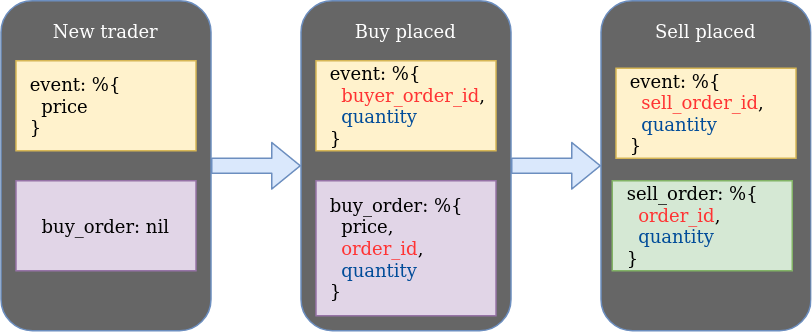
\includegraphics{images/chapter_02_01_trader_states.png}

Our trader will be receiving trade events sequentially and take decisions
based on it's own state and trade event's contents.

We will focus on a trader in 3 different states:
* a new trader without any orders
* a trader with a buy order placed
* a trader with a sell order placed.

\begin{itemize}
\tightlist
\item
  First state - A new trader
\end{itemize}

Trader doesn't have any open orders which we can confirm by pattern matching on the \texttt{buy\_order} field from its state. From the incoming event, we can get
the current price which we will use in the buy order that the trader will place.

\begin{itemize}
\tightlist
\item
  Second state - Buy order placed
\end{itemize}

After placing a buy order, trader will be pattern matching to confirm that
has incoming event filled his buy order otherwise ignoring it.
When trade event matching the order id of trader's buy order will arrive, it means that buy order got filled(simplification - our order could be filled in two or more transactions but implementation in this chapter won't cater for this case, it will always assume that it got filled in a single transaction) and trader can now place the sell order based on the expected profit and the buy\_price.

\begin{itemize}
\tightlist
\item
  Third state - Sell order placed
\end{itemize}

Finally, in a very similar fashion to previous state, the trader will be pattern matching to confirm that incoming event has filled his sell order(matching order id), otherwise ignoring it.
When trade event matching the order id of trader's sell order will arrive, that means that sell order got filled(simplification as described above) and full trade cycle has ended and the trader can now exit.

\hypertarget{implementation-of-the-first-scenario}{%
\subsection{Implementation of the first scenario}\label{implementation-of-the-first-scenario}}

Enough theory :) back to the editor, we will implement the first scenario. Before doing that let's alias Streamer's TradeEvent struct as we will rely on it heavily in pattern matching.

\begin{Shaded}
\begin{Highlighting}[]
  \CommentTok{\# /apps/naive/lib/naive/trader.ex}
  \ImportTok{alias} \ConstantTok{Streamer}\OperatorTok{.}\ConstantTok{Binance}\OperatorTok{.}\ConstantTok{TradeEvent}
\end{Highlighting}
\end{Shaded}

We are also aliasing the \texttt{\%Streamer.Binance.TradeEvent\{\}} struct as we will rely on it heavily in pattern matching.

To confirm that we are dealing with a ``new'' trader, we will pattern match on \texttt{buy\_order:\ nil} from it's state:

\begin{Shaded}
\begin{Highlighting}[]
  \CommentTok{\# /apps/naive/lib/naive/trader.ex}
  \KeywordTok{def}\NormalTok{ handle\_cast(}
\NormalTok{        \%}\ConstantTok{TradeEvent}\NormalTok{\{}\VariableTok{price:}\NormalTok{ price\},}
\NormalTok{        \%}\ConstantTok{State}\NormalTok{\{}\VariableTok{symbol:}\NormalTok{ symbol, }\VariableTok{buy\_order:} \ConstantTok{nil}\NormalTok{\} }\OperatorTok{=}\NormalTok{ state}
\NormalTok{      ) }\KeywordTok{do}
\NormalTok{    quantity }\OperatorTok{=} \DecValTok{100} \CommentTok{\# \textless{}= Hardcoded until chapter 7}

    \ConstantTok{Logger}\OperatorTok{.}\NormalTok{info(}\StringTok{"Placing BUY order for }\OtherTok{\#\{}\NormalTok{symbol}\OtherTok{\}}\StringTok{ @ }\OtherTok{\#\{}\NormalTok{price}\OtherTok{\}}\StringTok{, quantity: }\OtherTok{\#\{}\NormalTok{quantity}\OtherTok{\}}\StringTok{"}\NormalTok{)}

\NormalTok{    \{}\VariableTok{:ok}\NormalTok{, \%}\ConstantTok{Binance}\OperatorTok{.}\ConstantTok{OrderResponse}\NormalTok{\{\} }\OperatorTok{=}\NormalTok{ order\} }\OperatorTok{=}
      \ConstantTok{Binance}\OperatorTok{.}\NormalTok{order\_limit\_buy(symbol, quantity, price, }\StringTok{"GTC"}\NormalTok{)}

\NormalTok{    \{}\VariableTok{:noreply}\NormalTok{, \%\{state }\OperatorTok{|} \VariableTok{buy\_order:}\NormalTok{ order\}\}}
  \KeywordTok{end}
\end{Highlighting}
\end{Shaded}

For the time being, we will keep the quantity hardcoded as this chapter will
get really long otherwise - don't worry, we will refactor this in one of the next chapters.

After confirming that we deal with the ``new'' trader(by pattern matching on the \texttt{buy\_order} field from state), we can safely progress to placing a new buy order. We just need to remember to return the updated state as otherwise, trader will go on a shopping spree, as every next incoming event will cause further buy orders(above pattern match will continue to be successful).

\hypertarget{implementation-of-the-second-scenario}\ConstantTok{TradeEvent}\NormalTok{\{}
          \VariableTok{buyer\_order\_id:}\NormalTok{ order\_id,}
          \VariableTok{quantity:}\NormalTok{ quantity}
\NormalTok{        \},}
\NormalTok{        \%}\ConstantTok{State}\NormalTok{\{}
          \VariableTok{symbol:}\NormalTok{ symbol,}
          \VariableTok{buy\_order:}\NormalTok{ \%}\ConstantTok{Binance}\OperatorTok{.}\ConstantTok{OrderResponse}\NormalTok{\{}
            \VariableTok{price:}\NormalTok{ buy\_price,}
            \VariableTok{order\_id:}\NormalTok{ order\_id,}
            \VariableTok{orig\_qty:}\NormalTok{ quantity}
\NormalTok{          \},}
          \VariableTok{profit\_interval:}\NormalTok{ profit\_interval,}
          \VariableTok{tick\_size:}\NormalTok{ tick\_size}
\NormalTok{        \} }\OperatorTok{=}\NormalTok{ state}
\NormalTok{      ) }\KeywordTok{do}
\NormalTok{    sell\_price }\OperatorTok{=}\NormalTok{ calculate\_sell\_price(buy\_price, profit\_interval, tick\_size)}

    \ConstantTok{Logger}\OperatorTok{.}\NormalTok{info(}
      \StringTok{"Buy order filled, placing SELL order for "} \OperatorTok{\textless{}\textgreater{}}
        \StringTok{"}\OtherTok{\#\{}\NormalTok{symbol}\OtherTok{\}}\StringTok{ @ }\OtherTok{\#\{}\NormalTok{sell\_price}\OtherTok{\}}\StringTok{), quantity: }\OtherTok{\#\{}\NormalTok{quantity}\OtherTok{\}}\StringTok{"}
\NormalTok{    )}

\NormalTok{    \{}\VariableTok{:ok}\NormalTok{, \%}\ConstantTok{Binance}\OperatorTok{.}\ConstantTok{OrderResponse}\NormalTok{\{\} }\OperatorTok{=}\NormalTok{ order\} }\OperatorTok{=}
      \ConstantTok{Binance}\OperatorTok{.}\NormalTok{order\_limit\_sell(symbol, quantity, sell\_price, }\StringTok{"GTC"}\NormalTok{)}

\NormalTok{    \{}\VariableTok{:noreply}\NormalTok{, \%\{state }\OperatorTok{|} \VariableTok{sell\_order:}\NormalTok{ order\}\}}
  \KeywordTok{end}
\end{Highlighting}
\end{Shaded}

We will implement calculating sell price in a sepearate function based on buy price, profit interval and tick\_size.

Our pattern match will confirm that indeed our buy order got filled(order\_id and quantity matches) so we can now we proceed with placing a sell order using calculated sell price and quantity retrieved from buy order.
Again, don't forget to return the updated state as otherwise, trader will keep on placing sell orders for every incoming event.

To calculate the sell price we will need to use precise math and that will require a custom module. We will use the \href{https://github.com/ericmj/decimal}{Decimal} module, so first, let's alias it at the top of the file:

\begin{Shaded}
\begin{Highlighting}[]
\CommentTok{\# /apps/naive/lib/naive/trader.ex}
\ImportTok{alias} \ConstantTok{Decimal}\NormalTok{, }\VariableTok{as:}\NormalTok{ D}
\end{Highlighting}
\end{Shaded}

Now to calculate the correct sell price, we can use the following formula which gets me pretty close to expected value:

\begin{Shaded}
\begin{Highlighting}[]
  \CommentTok{\# /apps/naive/lib/naive/trader.ex}
  \KeywordTok{defp}\NormalTok{ calculate\_sell\_price(buy\_price, profit\_interval, tick\_size) }\KeywordTok{do}
\NormalTok{    fee }\OperatorTok{=}\NormalTok{ D}\OperatorTok{.}\NormalTok{new(}\StringTok{"1.001"}\NormalTok{)}
\NormalTok{    original\_price }\OperatorTok{=}\NormalTok{ D}\OperatorTok{.}\NormalTok{mult(D}\OperatorTok{.}\NormalTok{new(buy\_price), fee)}

\NormalTok{    net\_target\_price }\OperatorTok{=}
\NormalTok{      D}\OperatorTok{.}\NormalTok{mult(}
\NormalTok{        original\_price,}
\NormalTok{        D}\OperatorTok{.}\NormalTok{add(}\StringTok{"1.0"}\NormalTok{, profit\_interval)}
\NormalTok{      )}

\NormalTok{    gross\_target\_price }\OperatorTok{=}\NormalTok{ D}\OperatorTok{.}\NormalTok{mult(net\_target\_price, fee)}

\NormalTok{    D}\OperatorTok{.}\NormalTok{to\_float(}
\NormalTok{      D}\OperatorTok{.}\NormalTok{mult(}
\NormalTok{        D}\OperatorTok{.}\NormalTok{div\_int(gross\_target\_price, tick\_size),}
\NormalTok{        tick\_size}
\NormalTok{      )}
\NormalTok{    )}
  \KeywordTok{end}
\end{Highlighting}
\end{Shaded}

First, we would like to convert all the numbers to the \texttt{Decimal} structs so it will be easier to work with them. We will also hardcode the fee which we will refactor in one of the future chapters.

We started by calculating the \texttt{gross\_buy\_price} which is a sum of buy
price together with the fee that we paid on top of it.

Next, we enlarge the originally paid price by profit interval to get \texttt{net\_target\_price}

As we will be charged a fee for selling, we need to add the fee again on top of this target sell price(\texttt{gross\_target\_price}).

Next, we will use the tick size as Binance won't accept any prices that aren't divisible by the symbols' tick sizes so we need to ``normalize'' them on our side.

\hypertarget{implementation-of-the-third-scenario}\ConstantTok{TradeEvent}\NormalTok{\{}
          \VariableTok{seller\_order\_id:}\NormalTok{ order\_id,}
          \VariableTok{quantity:}\NormalTok{ quantity}
\NormalTok{        \},}
\NormalTok{        \%}\ConstantTok{State}\NormalTok{\{}
          \VariableTok{sell\_order:}\NormalTok{ \%}\ConstantTok{Binance}\OperatorTok{.}\ConstantTok{OrderResponse}\NormalTok{\{}
            \VariableTok{order\_id:}\NormalTok{ order\_id,}
            \VariableTok{orig\_qty:}\NormalTok{ quantity}
\NormalTok{          \}}
\NormalTok{        \} }\OperatorTok{=}\NormalTok{ state}
\NormalTok{      ) }\KeywordTok{do}
    \ConstantTok{Logger}\OperatorTok{.}\NormalTok{info(}\StringTok{"Trade finished, trader will now exit"}\NormalTok{)}
\NormalTok{    \{}\VariableTok{:stop}\NormalTok{, }\VariableTok{:normal}\NormalTok{, state\}}
  \KeywordTok{end}
\end{Highlighting}
\end{Shaded}

When the sell order was successfully filled(confirmed by pattern matching above), there's nothing else to do for the trader, so it can retrun a tuple with \texttt{:stop} atom which will cause the trader process to terminate.

\hypertarget{implementation-fallback-scenario}\ConstantTok{TradeEvent}\NormalTok{\{\}, state) }\KeywordTok{do}
\NormalTok{    \{}\VariableTok{:noreply}\NormalTok{, state\}}
  \KeywordTok{end}
\end{Highlighting}
\end{Shaded}

We need this callback for cases where our trader has an ``open'' order(not yet filled) and the incoming event has nothing to do with it, so it needs to be ignored.

\hypertarget{updating-the-naive-interface}{%
\subsection{Updating the Naive interface}\label{updating-the-naive-interface}}

Now we will update an interface of our \texttt{naive} application by modifying the Naive module to allow to send an event to the trader:

\begin{Shaded}
\begin{Highlighting}[]
\CommentTok{\# /apps/naive/lib/naive.ex}
\KeywordTok{defmodule} \ConstantTok{Naive} \KeywordTok{do}
  \OtherTok{@moduledoc """}
\CommentTok{  Documentation for }\InformationTok{\textasciigrave{}Naive\textasciigrave{}}\CommentTok{.}
\CommentTok{  }\OtherTok{"""}
  \ImportTok{alias} \ConstantTok{Streamer}\OperatorTok{.}\ConstantTok{Binance}\OperatorTok{.}\ConstantTok{TradeEvent}

  \KeywordTok{def}\NormalTok{ send\_event(\%}\ConstantTok{TradeEvent}\NormalTok{\{\} }\OperatorTok{=}\NormalTok{ event) }\KeywordTok{do}
    \ConstantTok{GenServer}\OperatorTok{.}\NormalTok{cast(}\VariableTok{:trader}\NormalTok{, event)}
  \KeywordTok{end}
\KeywordTok{end}
\end{Highlighting}
\end{Shaded}

We will use the fact that we registered our trader process with a name to be able to cast a message to it.

\hypertarget{updating-streamer-app}{%
\subsection{Updating streamer app}\label{updating-streamer-app}}

To glue our apps together for the time and keep things simple in this chapter we will modify the streamer process to simply call our new \texttt{Naive} interface directly by appending a following function call at the end of \texttt{process\_event/1} function inside the \texttt{Streamer.Binance} module:

\begin{Shaded}
\begin{Highlighting}[]
  \CommentTok{\# /apps/streamer/lib/streamer/binance.ex}
  \KeywordTok{defp}\NormalTok{ process\_event(\%\{}\StringTok{"e"} \OperatorTok{=\textgreater{}} \StringTok{"trade"}\NormalTok{\} }\OperatorTok{=}\NormalTok{ event) }\KeywordTok{do}
    \OperatorTok{...}
    \ConstantTok{Naive}\OperatorTok{.}\NormalTok{send\_event(trade\_event)}
  \KeywordTok{end}
\end{Highlighting}
\end{Shaded}

This creates a two way link between the streamer and the naive app. In the next chapter we will fix that as in the perfect world those apps shouldn't even be aware of existance of each other.

\hypertarget{access-details-to-binance}{%
\subsection{Access details to Binance}\label{access-details-to-binance}}

Inside the main config of our umbrella project we need to define access details for our Binance account:

\begin{Shaded}
\begin{Highlighting}[]
\NormalTok{config }\VariableTok{:binance}\NormalTok{,}
  \VariableTok{api\_key:} \StringTok{"YOUR{-}API{-}KEY{-}HERE"}\NormalTok{,}
  \VariableTok{secret\_key:} \StringTok{"YOUR{-}SECRET{-}KEY{-}HERE"}
\end{Highlighting}
\end{Shaded}

\emph{Important note}: To be able to run below test and perform real trades, Binance account is required with balance of at least 20 USDT. In the 4th chapter we will focus on creating a \texttt{BinanceMock} that will allow us to run our bot \emph{without} requirement for a real Binance account. You don't need to test run it now if you don't need/want to have an account.

\hypertarget{test-run}{%
\subsection{Test run}\label{test-run}}

Now it's the time to give our implementation a run for it's money. Once again, to be able to do that you will need to have at least 20 USDT tokens in your Binance's wallet and you will loose just under 0.5\% of your USDTs(as ``expected profit'' is below 0 to quickly showcase the full trade cycle) in the following test:

\begin{Shaded}
\begin{Highlighting}[]
\ExtensionTok{$}\NormalTok{ iex }\AttributeTok{{-}S}\NormalTok{ mix}
\ExtensionTok{...}
\ExtensionTok{iex}\ErrorTok{(}\ExtensionTok{1}\KeywordTok{)}\OperatorTok{\textgreater{}}\NormalTok{ Naive.Trader.start\_link}\KeywordTok{(}\ExtensionTok{\%\{symbol:} \StringTok{"XRPUSDT"}\NormalTok{, profit\_interval: Decimal.new}\ErrorTok{(}\StringTok{"{-}0.01"}\KeywordTok{)}\ErrorTok{\}}\KeywordTok{)}
\ExtensionTok{13:45:30.648}\NormalTok{ [info] Initializing new trader for XRPUSDT}
\ExtensionTok{\{:ok,} \CommentTok{\#PID\textless{}0.355.0\textgreater{}\}}
\ExtensionTok{iex}\ErrorTok{(}\ExtensionTok{2}\KeywordTok{)}\OperatorTok{\textgreater{}}\NormalTok{ Streamer.start\_streaming}\KeywordTok{(}\StringTok{"xrpusdt"}\KeywordTok{)}
\ExtensionTok{\{:ok,} \CommentTok{\#PID\textless{}0.372.0\textgreater{}\}}
\ExtensionTok{iex}\ErrorTok{(}\ExtensionTok{3}\KeywordTok{)}\OperatorTok{\textgreater{}} 
\ExtensionTok{13:45:32.561}\NormalTok{ [info] Placing BUY order for XRPUSDT @ 0.25979000, quantity: 100}
\ExtensionTok{13:45:32.831}\NormalTok{ [info] Buy order filled, placing SELL order for XRPUSDT @ 0.2577, quantity: 100}
\ExtensionTok{13:45:33.094}\NormalTok{ [info] Trade finished, trader will now exit}
\end{Highlighting}
\end{Shaded}

After starting the IEx session, start the trader process with a map containing symbol and profit interval. To be able to quickly test full trade cycle we will pass sub-zero profit interval instead of waiting for the increase in price.

Next, we will start streaming on the same symbol, please be aware that this will cause an immediate reaction in the trader process.

We can see that our trader placed a buy order at 25.979c per XRP, it was filled in under 300ms, so then the trader placed a sell order at \textasciitilde25.77c
which was also filled in under 300ms. This way the trader finished the trade
cycle and process can terminate.

That's it. Congratulations! You just made your first algorithmic trade and you should be proud of that! In the process of creating that algorithm we touched on multiple topics including GenServer and depending on it's state and external data (trade events) to perform different actions - this is a very common workflow that Elixir engineers are following and it's great to see it in action.

{[}Note{]} Please remember to run \texttt{mix\ format} to keep things nice and tidy.

Source code for this chapter can be found at \href{https://github.com/frathon/create-a-cryptocurrency-trading-bot-in-elixir-source-code/tree/chapter_02}{Github}

\hypertarget{introduce-pubsub-as-a-communication-method}{%
\chapter{Introduce PubSub as a communication method}\label{introduce-pubsub-as-a-communication-method}}

\hypertarget{objectives-2}{%
\section{Objectives}\label{objectives-2}}

\begin{itemize}
\tightlist
\item
  consider reasons why introducing a PubSub communication would be benefitial
\item
  implement the PubSub communication between the \texttt{Streamer.Binance} and the \texttt{Naive.Trader}(s)
\end{itemize}

\hypertarget{design}{%
\section{Design}\label{design}}

First, let's look at the current situation:

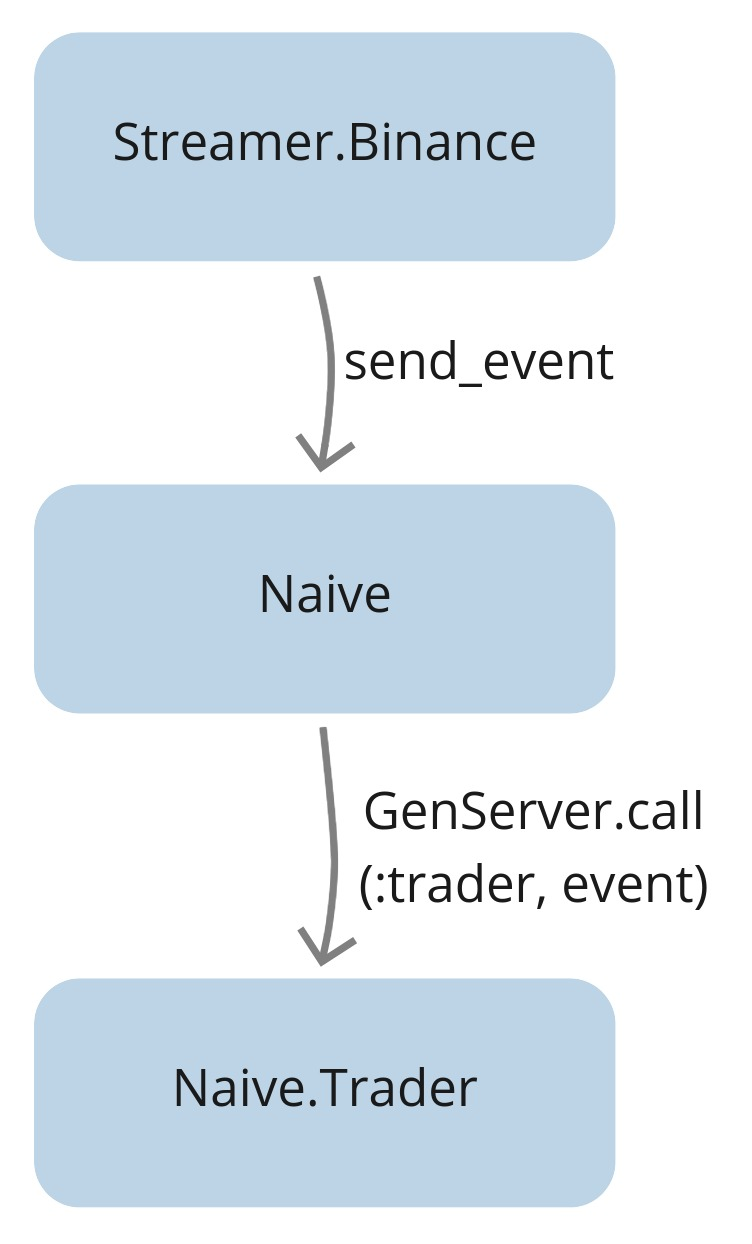
\includegraphics{images/chapter_03_01_current_situation.png}

We started with the Binance streamer calling the \texttt{send\_event/1} function on the \texttt{Naive} module. The \texttt{Naive} module then calls the trader process using the GenServer's \texttt{cast/2} function(via it's registered name).

Next step in the process of extending our trading strategy will be to scale it to run multiple \texttt{Naive.Trader} processes in parallel. To be able to do that we will need to remove the option to register the \texttt{trader} process with a name(as only one process can be registered under single name).

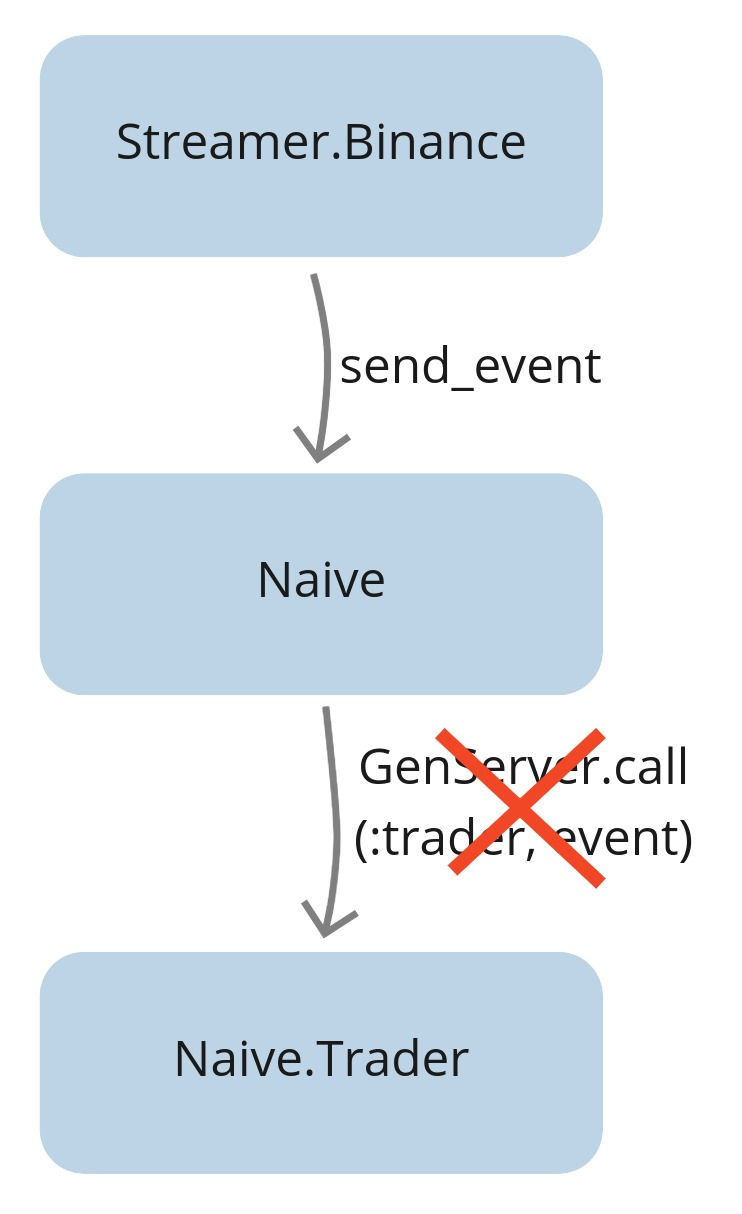
\includegraphics{images/chapter_03_02_current_situation_failed.png}

The second issue with that design was the fact that the \texttt{Streamer} needs to be aware of all processes that are interested in the streamed data and explicitly push that information to them.

To fix those issues we will invert the design and introduce a PubSub mechanism:

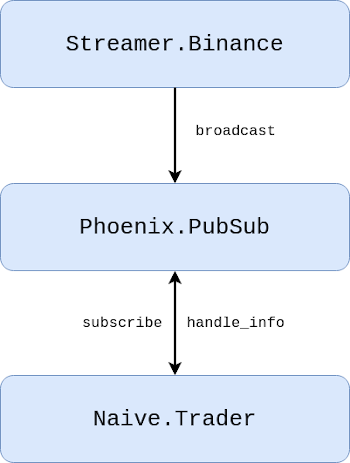
\includegraphics{images/chapter_03_03_phoenix_pubsub.png}

The streamer will broadcast trade events to the PubSub topic and whatever is interested in that data, can subscribe to the topic and it will receive the broadcasted messages.
There's no coupling between the \texttt{Streamer} and \texttt{Naive} app any more.

We can now introduce multiple traders that will subscribe to the topic and
they will receive messages from the PubSub:

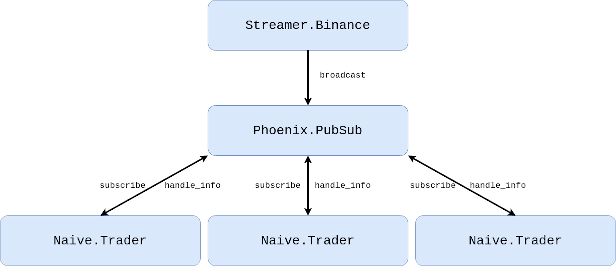
\includegraphics{images/chapter_03_04_naive_trader_group.png}

Going even further down the line we can picture that system could consist of other processes interested in the streamed data. Example of those could be a process that will save all streamed information to the database to be utilized in backtesting later on:

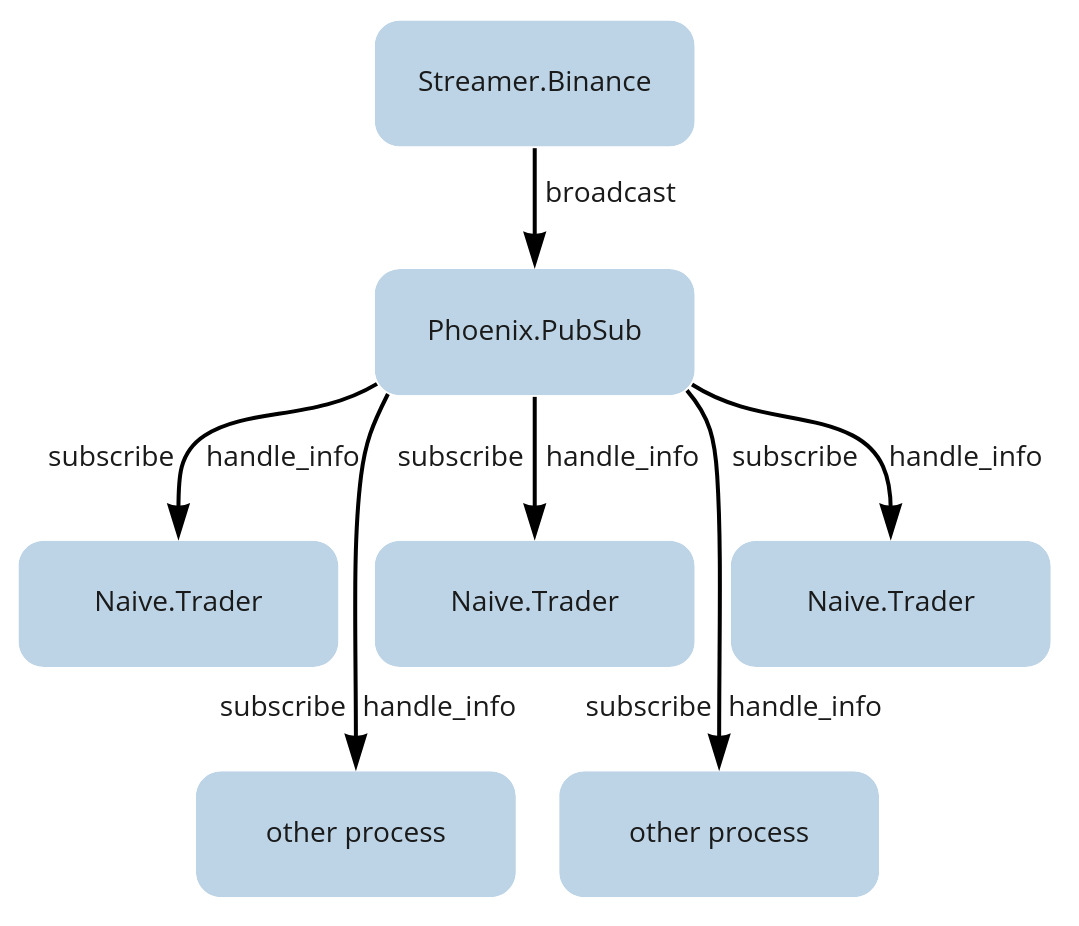
\includegraphics{images/chapter_03_05_other_services.png}

\hypertarget{implementation}{%
\section{Implementation}\label{implementation}}

We will start by adding a \href{https://github.com/phoenixframework/phoenix_pubsub}{\texttt{Phoenix.PubSub}} library to both \texttt{Streamer} and \texttt{Naive} app(as both will be using it, \texttt{Streamer} app as a broadcaster and \texttt{Naive} app as a subscriber)

Scrolling down through it's readme on GitHub we can see that we need to add \texttt{:phoenix\_pubsub} to list of dependencies:

\begin{Shaded}
\begin{Highlighting}[]
\CommentTok{\# /apps/streamer/mix.exs \& /apps/naive/mix.exs}
  \KeywordTok{defp}\NormalTok{ deps }\KeywordTok{do}
\NormalTok{    [}
      \OperatorTok{...}
\NormalTok{      \{}\VariableTok{:phoenix\_pubsub}\NormalTok{, }\StringTok{"\textasciitilde{}\textgreater{} 2.0"}\NormalTok{\},}
      \OperatorTok{...}
\NormalTok{    ]}
  \KeywordTok{end}
\end{Highlighting}
\end{Shaded}

Remember to place it so the list will keep alphabetical order. Second step in the readme says that we need to add PubSub as a child of our app. We need to decide where we will put it, \texttt{Streamer} sounds like a good starting point. We will modify the \texttt{/apps/streamer/lib/streamer/application.ex} module by appending the PubSub to it:

\begin{Shaded}
\begin{Highlighting}[]
\CommentTok{\# /apps/streamer/lib/streamer/application.ex}
  \KeywordTok{def}\NormalTok{ start(\_type, \_args) }\KeywordTok{do}
\NormalTok{    children }\OperatorTok{=}\NormalTok{ [}
\NormalTok{      \{}
        \ConstantTok{Phoenix}\OperatorTok{.}\ConstantTok{PubSub}\NormalTok{,}
        \VariableTok{name:} \ConstantTok{Streamer}\OperatorTok{.}\ConstantTok{PubSub}\NormalTok{, }\VariableTok{adapter\_name:} \ConstantTok{Phoenix}\OperatorTok{.}\ConstantTok{PubSub}\OperatorTok{.}\ConstantTok{PG2}
\NormalTok{      \}}
\NormalTok{    ]}
    \OperatorTok{...}
  \KeywordTok{end}
\end{Highlighting}
\end{Shaded}

We will add the \texttt{:adapter\_name} option to instruct PubSub to use \href{http://erlang.org/doc/man/pg.html}{\texttt{pg}} adapter, which will give us distrubuted process groups.

We will now modify the streamer to broadcast a message to PubSub topic instead of using the \texttt{Naive} module's function:

\begin{Shaded}
\begin{Highlighting}[]
\CommentTok{\# /apps/streamer/lib/streamer/binance.ex}
  \KeywordTok{defp}\NormalTok{ process\_event(}\OperatorTok{...}\NormalTok{) }\KeywordTok{do}
    \OperatorTok{...}

    \ConstantTok{Phoenix}\OperatorTok{.}\ConstantTok{PubSub}\OperatorTok{.}\NormalTok{broadcast(}
      \ConstantTok{Streamer}\OperatorTok{.}\ConstantTok{PubSub}\NormalTok{,}
      \StringTok{"TRADE\_EVENTS:}\OtherTok{\#\{}\NormalTok{trade\_event}\OperatorTok{.}\NormalTok{symbol}\OtherTok{\}}\StringTok{"}\NormalTok{,}
\NormalTok{      trade\_event}
\NormalTok{    )}
  \KeywordTok{end}
\end{Highlighting}
\end{Shaded}

Inside the trader on init we need to subscribe to the ``TRADE\_EVENTS'' PubSub channel:

\begin{Shaded}
\begin{Highlighting}[]
\CommentTok{\# /apps/naive/lib/naive/trader.ex}
  \KeywordTok{def}\NormalTok{ init(}\OperatorTok{...}\NormalTok{) }\KeywordTok{do}
    \OperatorTok{...}

    \ConstantTok{Phoenix}\OperatorTok{.}\ConstantTok{PubSub}\OperatorTok{.}\NormalTok{subscribe(}
      \ConstantTok{Streamer}\OperatorTok{.}\ConstantTok{PubSub}\NormalTok{,}
      \StringTok{"TRADE\_EVENTS:}\OtherTok{\#\{}\NormalTok{symbol}\OtherTok{\}}\StringTok{"}
\NormalTok{    )}

    \OperatorTok{...}
  \KeywordTok{end}
\end{Highlighting}
\end{Shaded}

Next, we need to convert all \texttt{handle\_call} callbacks to \texttt{handle\_info} inside our \texttt{Trader} module as PubSub doesn't use \texttt{GenServer.cast/2} to send messages over to subscribers.

The final change will be to remove the \texttt{send\_event} function from the \texttt{Naive}
module as it's no longer required.

Our update is now finished so we can start an iex session to see how it works.

First, we will start a streamer process that will broadcast messages
to PubSub. Next, we will start trading on the same symbol. On init, trader will subscribe to a PubSub channel and it will make a full trade cycle.

\begin{Shaded}
\begin{Highlighting}[]
\ExtensionTok{$}\NormalTok{ iex }\AttributeTok{{-}S}\NormalTok{ mix}
\ExtensionTok{...}
\ExtensionTok{iex}\ErrorTok{(}\ExtensionTok{1}\KeywordTok{)}\OperatorTok{\textgreater{}}\NormalTok{ Streamer.start\_streaming}\KeywordTok{(}\StringTok{"xrpusdt"}\KeywordTok{)}
\ExtensionTok{\{:ok,} \CommentTok{\#PID\textless{}0.483.0\textgreater{}\}}
\ExtensionTok{iex}\ErrorTok{(}\ExtensionTok{2}\KeywordTok{)}\OperatorTok{\textgreater{}}\NormalTok{ Naive.Trader.start\_link}\KeywordTok{(}\ExtensionTok{\%\{symbol:} \StringTok{"XRPUSDT"}\NormalTok{, profit\_interval: Decimal.new}\ErrorTok{(}\StringTok{"{-}0.01"}\KeywordTok{)}\ErrorTok{\}}\KeywordTok{)} 
\ExtensionTok{23:46:37.482}\NormalTok{ [info]  Initializing new trader for XRPUSDT}
\ExtensionTok{\{:ok,} \CommentTok{\#PID\textless{}0.474.0\textgreater{}\}}
\ExtensionTok{23:46:55.179}\NormalTok{ [info]  Placing BUY order for XRPUSDT @ 0.29462000, quantity: 100}
\ExtensionTok{23:46:55.783}\NormalTok{ [info]  Buy order filled, placing SELL order for XRPUSDT @ 0.29225}\ErrorTok{)}\ExtensionTok{,}\NormalTok{ quantity: 100.00000000}
\ExtensionTok{23:46:56.029}\NormalTok{ [info]  Trade finished, trader will now exit}
\end{Highlighting}
\end{Shaded}

This shows that new trader process successfully subscribed to the PubSub, received the broadcasted messages, placed buy/sell orders and terminated after full trade cycle finished.

{[}Note{]} Please remember to run \texttt{mix\ format} to keep things nice and tidy.

Source code for this chapter can be found at \href{https://github.com/frathon/create-a-cryptocurrency-trading-bot-in-elixir-source-code/tree/chapter_03}{Github}

\hypertarget{mock-the-binance-api}{%
\chapter{Mock the Binance API}\label{mock-the-binance-api}}

\hypertarget{objectives-3}{%
\section{Objectives}\label{objectives-3}}

\begin{itemize}
\tightlist
\item
  design the binance mock application
\item
  create a new app
\item
  implement getting exchange info
\item
  implement placing buy and sell orders
\item
  implement callback for incoming trade events
\item
  upgrade trader and config
\item
  test the implementation
\end{itemize}

\hypertarget{design-1}{%
\section{Design}\label{design-1}}

First, let's start with the current state:

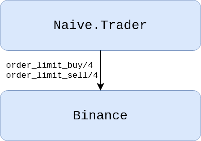
\includegraphics{images/chapter_04_01_current_state.png}

Currently our trader is using the \texttt{Binance} module to place buy/sell
orders and get exchange info.
The \texttt{get\_exchange\_info/0} function doesn't require a Binance account as it's a publicly available information so we can call the \texttt{Binance} lib directly from our module.
The remaining ones(buying/selling) require \texttt{Binance} account and some coins/token inside it's wallet. We need to mock those inside our module.

We will update the trader to fetch the Binance's module name from the config:

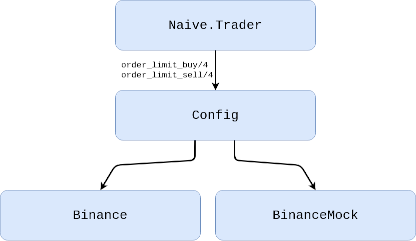
\includegraphics{images/chapter_04_02_proposal.png}

We will set up a config so it points to the Binance client to be used - either Binance or BinanceMock. Regards the BinanceMock itself it will have the same interface as the Binance module.
It will need to store both buy and sell orders and it will allow us to retrieve them. That will cover the REST functions but Binance also streams back trade events for those orders as they get filled, that's why BinanceMock will also need to broadcast fake events to the ``TRADE\_EVENTS:\#\{symbol\}'' PubSub topic so the trader will pick them up:

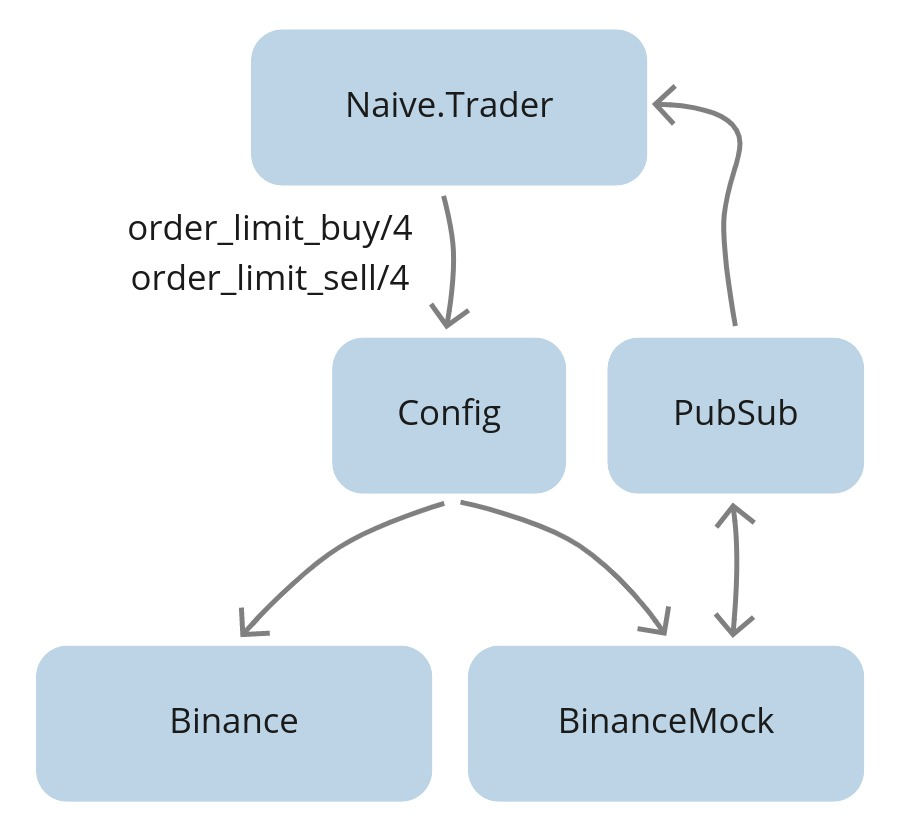
\includegraphics{images/chapter_04_03_proposal_pubsub.png}

When exactly should we broadcast those fake trade events? Well, the best thing
that we can do is make \texttt{BinanceMock} process to subscribe to the trade events stream and try to broadcast fake trade events whenever the price of orders would be matched:

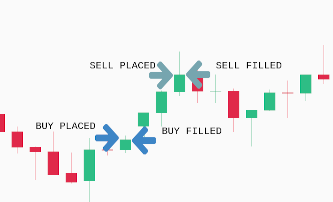
\includegraphics{images/chapter_04_04_explenation.png}

Starting from the arrow on the left, our naive strategy will place an order at the current price.
In this hypotetical scenario price was raising for a moment after placing the buy order, so BinanceMock will keep on waiting until a trade event will get broadcasted from the PubSub with price \emph{below} the buy order's price. At that moment BinanceMock will generate a fake trade event and broadcast it to the same PubSub topic.
Trader will get that event and assume that it came from the Binance and that the buy order got filled so it will place a sell order.
Similarly to the buy order, BinanceMock will keep on waiting until a trade event will get broadcasted from the PubSub with the price \emph{above} the sell order's price. At that moment BinanceMock will generate a fake trade event and broadcast it to the same PubSub topic.

Enough theory for now, let's get our hands dirty with some coding

\hypertarget{create-binancemock-app}{%
\section{Create ``BinanceMock'' app}\label{create-binancemock-app}}

We will start by creating a new supervised app called \texttt{BinanceMock}:

\begin{Shaded}
\begin{Highlighting}[]
\ExtensionTok{$}\NormalTok{ cd apps}
\ExtensionTok{$}\NormalTok{ mix new binance\_mock }\AttributeTok{{-}{-}sup}
\end{Highlighting}
\end{Shaded}

The next step will be to update the \texttt{BinanceMock} module to be a GenServer.

We will utilize:
* the \texttt{Decimal} module for comparing the prices
* the \texttt{Logger} module to log

As well as we will define internal \texttt{\%State\{\}} struct that will hold:
- map called \texttt{order\_books} for each traded symbol
- list of symbols that mock subscribed to
- last generated id - for consistent generating of unique ids for fake trade events

\texttt{order\_books} map will consist of \texttt{:"\#\{symbol\}} =\textgreater{} \texttt{\%OrderBook\{\}}. We will define the \texttt{\%OrderBook\{\}} struct as 3 lists \texttt{buy\_side}, \texttt{sell\_side} and \texttt{historical}:

\begin{Shaded}
\begin{Highlighting}[]
\CommentTok{\# /apps/binance\_mock/lib/binance\_mock.ex}
\KeywordTok{defmodule} \ConstantTok{BinanceMock} \KeywordTok{do}
  \ImportTok{use} \ConstantTok{GenServer}

  \ImportTok{alias} \ConstantTok{Decimal}\NormalTok{, }\VariableTok{as:}\NormalTok{ D}

  \ImportTok{require} \ConstantTok{Logger}

  \KeywordTok{defmodule} \ConstantTok{State} \KeywordTok{do}
    \KeywordTok{defstruct} \VariableTok{order\_books:}\NormalTok{ \%\{\}, }\VariableTok{subscriptions:}\NormalTok{ [], }\VariableTok{fake\_order\_id:} \DecValTok{1}
  \KeywordTok{end}

  \KeywordTok{defmodule} \ConstantTok{OrderBook} \KeywordTok{do}
    \KeywordTok{defstruct} \VariableTok{buy\_side:}\NormalTok{ [], }\VariableTok{sell\_side:}\NormalTok{ [], }\VariableTok{historical:}\NormalTok{ []}
  \KeywordTok{end}  

  \KeywordTok{def}\NormalTok{ start\_link(\_args) }\KeywordTok{do}
    \ConstantTok{GenServer}\OperatorTok{.}\NormalTok{start\_link(}\ConstantTok{\_\_MODULE\_\_}\NormalTok{, }\ConstantTok{nil}\NormalTok{, }\VariableTok{name:} \ConstantTok{\_\_MODULE\_\_}\NormalTok{)}
  \KeywordTok{end}

  \KeywordTok{def}\NormalTok{ init(\_args) }\KeywordTok{do}
\NormalTok{    \{}\VariableTok{:ok}\NormalTok{, \%}\ConstantTok{State}\NormalTok{\{\}\}}
  \KeywordTok{end}
\KeywordTok{end}
\end{Highlighting}
\end{Shaded}

\hypertarget{implement-getting-exchange-info}{%
\section{Implement getting exchange info}\label{implement-getting-exchange-info}}

As it was mentioned before, to retrieve exchange info we can just call Binance's function directly as it's a publicly avaiable information:

\begin{Shaded}
\begin{Highlighting}[]
\CommentTok{\# /apps/binance\_mock/lib/binance\_mock.ex}
  \KeywordTok{def}\NormalTok{ get\_exchange\_info() }\KeywordTok{do}
    \ConstantTok{Binance}\OperatorTok{.}\NormalTok{get\_exchange\_info()}
  \KeywordTok{end}
\end{Highlighting}
\end{Shaded}

\hypertarget{implement-placing-buy-and-sell-orders}{%
\section{Implement placing buy and sell orders}\label{implement-placing-buy-and-sell-orders}}

For buy and sell limit orders we will write a helper function as the logic is
the same for both order sides:

\begin{Shaded}
\begin{Highlighting}[]
\CommentTok{\# /apps/binance\_mock/lib/binance\_mock.ex}
  \KeywordTok{def}\NormalTok{ order\_limit\_buy(symbol, quantity, price, }\StringTok{"GTC"}\NormalTok{) }\KeywordTok{do}
\NormalTok{    order\_limit(symbol, quantity, price, }\StringTok{"BUY"}\NormalTok{)}
  \KeywordTok{end}

  \KeywordTok{def}\NormalTok{ order\_limit\_sell(symbol, quantity, price, }\StringTok{"GTC"}\NormalTok{) }\KeywordTok{do}
\NormalTok{    order\_limit(symbol, quantity, price, }\StringTok{"SELL"}\NormalTok{)}
  \KeywordTok{end}
\end{Highlighting}
\end{Shaded}

The ``order\_limit'' helper function will:
- ensure that quantity and price are float values as the \texttt{Binance} module accepts both strings and floats
- generate a fake order based on symbol, quantity, price, and side
- cast a message to the BinanceMock process to add the fake order
- return with a tuple with \texttt{\%OrderResponse\{\}} struct to be consistent with the Binance module:

\begin{Shaded}
\begin{Highlighting}[]
\CommentTok{\# /apps/binance\_mock/lib/binance\_mock.ex}
  \KeywordTok{defp}\NormalTok{ order\_limit(symbol, quantity, price, side) }\KeywordTok{do}
\NormalTok{    quantity }\OperatorTok{=} \ConstantTok{Float}\OperatorTok{.}\NormalTok{parse(}\StringTok{"}\OtherTok{\#\{}\NormalTok{quantity}\OtherTok{\}}\StringTok{"}\NormalTok{) }\OperatorTok{|\textgreater{}}\NormalTok{ elem(}\DecValTok{0}\NormalTok{)}
\NormalTok{    price }\OperatorTok{=} \ConstantTok{Float}\OperatorTok{.}\NormalTok{parse(}\StringTok{"}\OtherTok{\#\{}\NormalTok{price}\OtherTok{\}}\StringTok{"}\NormalTok{) }\OperatorTok{|\textgreater{}}\NormalTok{ elem(}\DecValTok{0}\NormalTok{)}

\NormalTok{    \%}\ConstantTok{Binance}\OperatorTok{.}\ConstantTok{Order}\NormalTok{\{\} }\OperatorTok{=}
\NormalTok{      fake\_order }\OperatorTok{=}
\NormalTok{      generate\_fake\_order(}
\NormalTok{        symbol,}
\NormalTok{        quantity,}
\NormalTok{        price,}
\NormalTok{        side}
\NormalTok{      )}

    \ConstantTok{GenServer}\OperatorTok{.}\NormalTok{cast(}
      \ConstantTok{\_\_MODULE\_\_}\NormalTok{,}
\NormalTok{      \{}\VariableTok{:add\_order}\NormalTok{, fake\_order\}}
\NormalTok{    )}

\NormalTok{    \{}\VariableTok{:ok}\NormalTok{, convert\_order\_to\_order\_response(fake\_order)\}}
  \KeywordTok{end}
\end{Highlighting}
\end{Shaded}

We can now move on to the implementation of the \texttt{handle\_cast/2} callback to \texttt{:add\_order} to the order book for the symbol from the order.
It needs to do two things:
- subscribe to the \texttt{TRADE\_EVENTS:\#\{symbol\}} topic for the symbol from
the order
- add the order to the correct order book

\begin{Shaded}
\begin{Highlighting}[]
\CommentTok{\# /apps/binance\_mock/lib/binance\_mock.ex}
  \KeywordTok{def}\NormalTok{ handle\_cast(}
\NormalTok{        \{}\VariableTok{:add\_order}\NormalTok{, \%}\ConstantTok{Binance}\OperatorTok{.}\ConstantTok{Order}\NormalTok{\{}\VariableTok{symbol:}\NormalTok{ symbol\} }\OperatorTok{=}\NormalTok{ order\},}
\NormalTok{        \%}\ConstantTok{State}\NormalTok{\{}
          \VariableTok{order\_books:}\NormalTok{ order\_books,}
          \VariableTok{subscriptions:}\NormalTok{ subscriptions}
\NormalTok{        \} }\OperatorTok{=}\NormalTok{ state}
\NormalTok{      ) }\KeywordTok{do}
\NormalTok{    new\_subscriptions }\OperatorTok{=}\NormalTok{ subscribe\_to\_topic(symbol, subscriptions)}
\NormalTok{    updated\_order\_books }\OperatorTok{=}\NormalTok{ add\_order(order, order\_books)}

\NormalTok{    \{}
      \VariableTok{:noreply}\NormalTok{,}
\NormalTok{      \%\{}
\NormalTok{        state}
        \OperatorTok{|} \VariableTok{order\_books:}\NormalTok{ updated\_order\_books,}
          \VariableTok{subscriptions:}\NormalTok{ new\_subscriptions}
\NormalTok{      \}}
\NormalTok{    \}}
  \KeywordTok{end}
\end{Highlighting}
\end{Shaded}

We will start with the implementation of \texttt{subscribe\_to\_topic/2} function. We need to make sure that the symbol is uppercase'd as well as check have we already subscribed to that topic. Otherwise, we can safely use the PubSub module to subscribe to the \texttt{TRADE\_EVENTS:\#\{symbol\}} topic for this symbol.
We need to remember to append the symbol to the list of subscription and return the updated list:

\begin{Shaded}
\begin{Highlighting}[]
\CommentTok{\# /apps/binance\_mock/lib/binance\_mock.ex}
  \KeywordTok{defp}\NormalTok{ subscribe\_to\_topic(symbol, subscriptions) }\KeywordTok{do}
\NormalTok{    symbol }\OperatorTok{=} \ConstantTok{String}\OperatorTok{.}\NormalTok{upcase(symbol)}
\NormalTok{    stream\_name }\OperatorTok{=} \StringTok{"TRADE\_EVENTS:}\OtherTok{\#\{}\NormalTok{symbol}\OtherTok{\}}\StringTok{"}

    \KeywordTok{case} \ConstantTok{Enum}\OperatorTok{.}\NormalTok{member?(subscriptions, symbol) }\KeywordTok{do}
      \ConstantTok{false} \OperatorTok{{-}\textgreater{}}
        \ConstantTok{Logger}\OperatorTok{.}\NormalTok{debug(}\StringTok{"BinanceMock subscribing to }\OtherTok{\#\{}\NormalTok{stream\_name}\OtherTok{\}}\StringTok{"}\NormalTok{)}

        \ConstantTok{Phoenix}\OperatorTok{.}\ConstantTok{PubSub}\OperatorTok{.}\NormalTok{subscribe(}
          \ConstantTok{Streamer}\OperatorTok{.}\ConstantTok{PubSub}\NormalTok{,}
\NormalTok{          stream\_name}
\NormalTok{        )}

\NormalTok{        [symbol }\OperatorTok{|}\NormalTok{ subscriptions]}

\NormalTok{      \_ }\OperatorTok{{-}\textgreater{}}
\NormalTok{        subscriptions}
    \KeywordTok{end}
  \KeywordTok{end}
\end{Highlighting}
\end{Shaded}

Next, time for implementation of \texttt{add\_order} function. First, we need to get the order book for the symbol of the order. Depends on the side of the order we will update either \texttt{buy\_side} or \texttt{sell\_side} list remembering that both sides are sorted. We are sorting them so we can easily grab all orders that should be filled whenever trade event arrived, this will become clearer as we will write a handle callback for incoming trade events:

\begin{Shaded}
\begin{Highlighting}[]
\CommentTok{\# /apps/binance\_mock/lib/binance\_mock.ex}
  \KeywordTok{defp}\NormalTok{ add\_order(}
\NormalTok{         \%}\ConstantTok{Binance}\OperatorTok{.}\ConstantTok{Order}\NormalTok{\{}\VariableTok{symbol:}\NormalTok{ symbol\} }\OperatorTok{=}\NormalTok{ order,}
\NormalTok{         order\_books}
\NormalTok{       ) }\KeywordTok{do}
\NormalTok{    order\_book }\OperatorTok{=}
      \ConstantTok{Map}\OperatorTok{.}\NormalTok{get(}
\NormalTok{        order\_books,}
\NormalTok{        :}\StringTok{"}\OtherTok{\#\{}\NormalTok{symbol}\OtherTok{\}}\StringTok{"}\NormalTok{,}
\NormalTok{        \%}\ConstantTok{OrderBook}\NormalTok{\{\}}
\NormalTok{      )}

\NormalTok{    order\_book }\OperatorTok{=}
      \ControlFlowTok{if}\NormalTok{ order}\OperatorTok{.}\NormalTok{side }\OperatorTok{==} \StringTok{"SELL"} \KeywordTok{do}
        \ConstantTok{Map}\OperatorTok{.}\NormalTok{replace!(}
\NormalTok{          order\_book,}
          \VariableTok{:sell\_side}\NormalTok{,}
\NormalTok{          [order }\OperatorTok{|}\NormalTok{ order\_book}\OperatorTok{.}\NormalTok{sell\_side]}
          \OperatorTok{|\textgreater{}} \ConstantTok{Enum}\OperatorTok{.}\NormalTok{sort(}\OperatorTok{\&}\NormalTok{D}\OperatorTok{.}\NormalTok{lt?(D}\OperatorTok{.}\NormalTok{new(}\OperatorTok{\&}\DecValTok{1}\OperatorTok{.}\NormalTok{price), D}\OperatorTok{.}\NormalTok{new(}\OperatorTok{\&}\DecValTok{2}\OperatorTok{.}\NormalTok{price)))}
\NormalTok{        )}
      \ControlFlowTok{else}
        \ConstantTok{Map}\OperatorTok{.}\NormalTok{replace!(}
\NormalTok{          order\_book,}
          \VariableTok{:buy\_side}\NormalTok{,}
\NormalTok{          [order }\OperatorTok{|}\NormalTok{ order\_book}\OperatorTok{.}\NormalTok{buy\_side]}
          \OperatorTok{|\textgreater{}} \ConstantTok{Enum}\OperatorTok{.}\NormalTok{sort(}\OperatorTok{\&}\NormalTok{D}\OperatorTok{.}\NormalTok{gt?(D}\OperatorTok{.}\NormalTok{new(}\OperatorTok{\&}\DecValTok{1}\OperatorTok{.}\NormalTok{price), D}\OperatorTok{.}\NormalTok{new(}\OperatorTok{\&}\DecValTok{2}\OperatorTok{.}\NormalTok{price)))}
\NormalTok{        )}
      \KeywordTok{end}

    \ConstantTok{Map}\OperatorTok{.}\NormalTok{put(order\_books, :}\StringTok{"}\OtherTok{\#\{}\NormalTok{symbol}\OtherTok{\}}\StringTok{"}\NormalTok{, order\_book)}
  \KeywordTok{end}
\end{Highlighting}
\end{Shaded}

Now we need to follow up and implement the functions that we referred to
previously - those are \texttt{generate\_fake\_order} and \texttt{convert\_order\_to\_order\_response}.

Starting with the \texttt{generate\_fake\_orders}, it's a function that takes a symbol, quantity, price and side and based on those values returns a \texttt{Binance.Order} struct. To return the struct we will need to generate a unique id for each faked order - this is where \texttt{fake\_order\_id} will be used(callback implemented later). This way we will be able to run tests multiple times using the BinanceMock and always get the same ids:

\begin{Shaded}
\begin{Highlighting}[]
\CommentTok{\# /apps/binance\_mock/lib/binance\_mock.ex}
  \KeywordTok{defp}\NormalTok{ generate\_fake\_order(symbol, quantity, price, side)}
       \KeywordTok{when}\NormalTok{ is\_binary(symbol) }\KeywordTok{and}
\NormalTok{              is\_float(quantity) }\KeywordTok{and}
\NormalTok{              is\_float(price) }\KeywordTok{and}
\NormalTok{              (side }\OperatorTok{==} \StringTok{"BUY"} \KeywordTok{or}\NormalTok{ side }\OperatorTok{==} \StringTok{"SELL"}\NormalTok{) }\KeywordTok{do}
\NormalTok{    current\_timestamp }\OperatorTok{=} \VariableTok{:os}\OperatorTok{.}\NormalTok{system\_time(}\VariableTok{:millisecond}\NormalTok{)}
\NormalTok{    order\_id }\OperatorTok{=} \ConstantTok{GenServer}\OperatorTok{.}\NormalTok{call(}\ConstantTok{\_\_MODULE\_\_}\NormalTok{, }\VariableTok{:generate\_id}\NormalTok{)}
\NormalTok{    client\_order\_id }\OperatorTok{=} \VariableTok{:crypto}\OperatorTok{.}\NormalTok{hash(}\VariableTok{:md5}\NormalTok{, }\StringTok{"}\OtherTok{\#\{}\NormalTok{order\_id}\OtherTok{\}}\StringTok{"}\NormalTok{) }\OperatorTok{|\textgreater{}} \ConstantTok{Base}\OperatorTok{.}\NormalTok{encode16()}

    \ConstantTok{Binance}\OperatorTok{.}\ConstantTok{Order}\OperatorTok{.}\NormalTok{new(\%\{}
      \VariableTok{symbol:}\NormalTok{ symbol,}
      \VariableTok{order\_id:}\NormalTok{ order\_id,}
      \VariableTok{client\_order\_id:}\NormalTok{ client\_order\_id,}
      \VariableTok{price:} \ConstantTok{Float}\OperatorTok{.}\NormalTok{to\_string(price),}
      \VariableTok{orig\_qty:} \ConstantTok{Float}\OperatorTok{.}\NormalTok{to\_string(quantity),}
      \VariableTok{executed\_qty:} \StringTok{"0.00000000"}\NormalTok{,}
      \VariableTok{cummulative\_quote\_qty:} \StringTok{"0.00000000"}\NormalTok{,}
      \VariableTok{status:} \StringTok{"NEW"}\NormalTok{,}
      \VariableTok{time\_in\_force:} \StringTok{"GTC"}\NormalTok{,}
      \VariableTok{type:} \StringTok{"LIMIT"}\NormalTok{,}
      \VariableTok{side:}\NormalTok{ side,}
      \VariableTok{stop\_price:} \StringTok{"0.00000000"}\NormalTok{,}
      \VariableTok{iceberg\_qty:} \StringTok{"0.00000000"}\NormalTok{,}
      \VariableTok{time:}\NormalTok{ current\_timestamp,}
      \VariableTok{update\_time:}\NormalTok{ current\_timestamp,}
      \VariableTok{is\_working:} \ConstantTok{true}
\NormalTok{    \})}
  \KeywordTok{end}
\end{Highlighting}
\end{Shaded}

We can now focus on converting the \texttt{Binance.Order} to the \texttt{Binance.OrderResponse} struct. As \texttt{Binance.Order} struct contains almost all of the same fields that the \texttt{Binance.OrderResponse} struct, we can use \texttt{struct} function without exclanation mark to ignore all additional fields. The only field that has different name is \texttt{transact\_time} field which is called \texttt{time} in the \texttt{Binance.Order} struct - we can fix that separetely:

\begin{Shaded}
\begin{Highlighting}[]
\CommentTok{\# /apps/binance\_mock/lib/binance\_mock.ex}
  \KeywordTok{defp}\NormalTok{ convert\_order\_to\_order\_response(\%}\ConstantTok{Binance}\OperatorTok{.}\ConstantTok{Order}\NormalTok{\{\} }\OperatorTok{=}\NormalTok{ order) }\KeywordTok{do}
\NormalTok{    \%\{}
\NormalTok{      struct(}
        \ConstantTok{Binance}\OperatorTok{.}\ConstantTok{OrderResponse}\NormalTok{,}
\NormalTok{        order }\OperatorTok{|\textgreater{}} \ConstantTok{Map}\OperatorTok{.}\NormalTok{to\_list()}
\NormalTok{      )}
      \OperatorTok{|} \VariableTok{transact\_time:}\NormalTok{ order}\OperatorTok{.}\NormalTok{time}
\NormalTok{    \}}
  \KeywordTok{end}
\end{Highlighting}
\end{Shaded}

Last function to finish support for placing buy and sell orders is to add a callback that will iterate the fake order id and return it:

\begin{Shaded}
\begin{Highlighting}[]
\CommentTok{\# /apps/binance\_mock/lib/binance\_mock.ex}
  \KeywordTok{def}\NormalTok{ handle\_call(}
        \VariableTok{:generate\_id}\NormalTok{,}
\NormalTok{        \_from,}
\NormalTok{        \%}\ConstantTok{State}\NormalTok{\{}\VariableTok{fake\_order\_id:}\NormalTok{ id\} }\OperatorTok{=}\NormalTok{ state}
\NormalTok{      ) }\KeywordTok{do}
\NormalTok{    \{}\VariableTok{:reply}\NormalTok{, id }\OperatorTok{+} \DecValTok{1}\NormalTok{, \%\{state }\OperatorTok{|} \VariableTok{fake\_order\_id:}\NormalTok{ id }\OperatorTok{+} \DecValTok{1}\NormalTok{\}\}}
  \KeywordTok{end}
\end{Highlighting}
\end{Shaded}

\hypertarget{implement-order-retrival}{%
\section{Implement order retrival}\label{implement-order-retrival}}

We can now move on to retrieving the orders. First, we need to add an interface function that will call our BinanceMock genserver:

\begin{Shaded}
\begin{Highlighting}[]
\CommentTok{\# /apps/binance\_mock/lib/binance\_mock.ex}
  \KeywordTok{def}\NormalTok{ get\_order(symbol, time, order\_id) }\KeywordTok{do}
    \ConstantTok{GenServer}\OperatorTok{.}\NormalTok{call(}
      \ConstantTok{\_\_MODULE\_\_}\NormalTok{,}
\NormalTok{      \{}\VariableTok{:get\_order}\NormalTok{, symbol, time, order\_id\}}
\NormalTok{    )}
  \KeywordTok{end}
\end{Highlighting}
\end{Shaded}

The callback itself is pretty straightforward. We will need to get order book for passed symbol. As we don't know the order's side, we will concat all 3 lists(buy\_side, sell\_side and historical) and try to find an order that will
match passed symbol, time and order\_id:

\begin{Shaded}
\begin{Highlighting}[]
\CommentTok{\# /apps/binance\_mock/lib/binance\_mock.ex}
  \KeywordTok{def}\NormalTok{ handle\_call(}
\NormalTok{        \{}\VariableTok{:get\_order}\NormalTok{, symbol, time, order\_id\},}
\NormalTok{        \_from,}
\NormalTok{        \%}\ConstantTok{State}\NormalTok{\{}\VariableTok{order\_books:}\NormalTok{ order\_books\} }\OperatorTok{=}\NormalTok{ state}
\NormalTok{      ) }\KeywordTok{do}
\NormalTok{    order\_book }\OperatorTok{=}
      \ConstantTok{Map}\OperatorTok{.}\NormalTok{get(}
\NormalTok{        order\_books,}
\NormalTok{        :}\StringTok{"}\OtherTok{\#\{}\NormalTok{symbol}\OtherTok{\}}\StringTok{"}\NormalTok{,}
\NormalTok{        \%}\ConstantTok{OrderBook}\NormalTok{\{\}}
\NormalTok{      )}

\NormalTok{    result }\OperatorTok{=}
\NormalTok{      (order\_book}\OperatorTok{.}\NormalTok{buy\_side }\OperatorTok{++}
\NormalTok{         order\_book}\OperatorTok{.}\NormalTok{sell\_side }\OperatorTok{++}
\NormalTok{         order\_book}\OperatorTok{.}\NormalTok{historical)}
      \OperatorTok{|\textgreater{}} \ConstantTok{Enum}\OperatorTok{.}\NormalTok{find(}
        \OperatorTok{\&}\NormalTok{(}\OperatorTok{\&}\DecValTok{1}\OperatorTok{.}\NormalTok{symbol }\OperatorTok{==}\NormalTok{ symbol }\KeywordTok{and}
            \OperatorTok{\&}\DecValTok{1}\OperatorTok{.}\NormalTok{time }\OperatorTok{==}\NormalTok{ time }\KeywordTok{and}
            \OperatorTok{\&}\DecValTok{1}\OperatorTok{.}\NormalTok{order\_id }\OperatorTok{==}\NormalTok{ order\_id)}
\NormalTok{      )}

\NormalTok{    \{}\VariableTok{:reply}\NormalTok{, \{}\VariableTok{:ok}\NormalTok{, result\}, state\}}
  \KeywordTok{end}
\end{Highlighting}
\end{Shaded}

\hypertarget{implement-callback-for-incoming-trade-events}{%
\section{Implement callback for incoming trade events}\label{implement-callback-for-incoming-trade-events}}

Finally, we need to handle incoming trade events(streamed from the PubSub topic). We need to implement a callback that will:
- get the order book for the symbol from the trade event
- use the \texttt{take\_while/2} function on the buy orders with prices that are \emph{greater} than the current price - we can update their status to filled.
- use the \texttt{take\_while/2} function again, this time to sell orders with prices \emph{less} than the current price, we will also update their statuses to filled.
- concat both lists of filled orders, convert them to trade events and broadcast them to the PubSub's TRADE\_EVENTS topic.
- remove the filled orders from buy and sell lists and put them into the historical list.

Here we can clearly see the benefit of sorting the lists, we can use functions like \texttt{take\_while/2} and \texttt{drop/2} instead of \texttt{filter/2}
and \texttt{reject/2}(later ones will go through whole lists which could become a bottleneck when multiple open orders would be active):

\begin{Shaded}
\begin{Highlighting}[]
\CommentTok{\# /apps/binance\_mock/lib/binance\_mock.ex}
  \KeywordTok{def}\NormalTok{ handle\_info(}
\NormalTok{        \%}\ConstantTok{Streamer}\OperatorTok{.}\ConstantTok{Binance}\OperatorTok{.}\ConstantTok{TradeEvent}\NormalTok{\{\} }\OperatorTok{=}\NormalTok{ trade\_event,}
\NormalTok{        \%\{}\VariableTok{order\_books:}\NormalTok{ order\_books\} }\OperatorTok{=}\NormalTok{ state}
\NormalTok{      ) }\KeywordTok{do}
\NormalTok{    order\_book }\OperatorTok{=}
      \ConstantTok{Map}\OperatorTok{.}\NormalTok{get(}
\NormalTok{        order\_books,}
\NormalTok{        :}\StringTok{"}\OtherTok{\#\{}\NormalTok{trade\_event}\OperatorTok{.}\NormalTok{symbol}\OtherTok{\}}\StringTok{"}\NormalTok{,}
\NormalTok{        \%}\ConstantTok{OrderBook}\NormalTok{\{\}}
\NormalTok{      )}

\NormalTok{    filled\_buy\_orders }\OperatorTok{=}
\NormalTok{      order\_book}\OperatorTok{.}\NormalTok{buy\_side}
      \OperatorTok{|\textgreater{}} \ConstantTok{Enum}\OperatorTok{.}\NormalTok{take\_while(}\OperatorTok{\&}\NormalTok{D}\OperatorTok{.}\NormalTok{lt?(D}\OperatorTok{.}\NormalTok{new(trade\_event}\OperatorTok{.}\NormalTok{price), D}\OperatorTok{.}\NormalTok{new(}\OperatorTok{\&}\DecValTok{1}\OperatorTok{.}\NormalTok{price)))}
      \OperatorTok{|\textgreater{}} \ConstantTok{Enum}\OperatorTok{.}\NormalTok{map(}\OperatorTok{\&}\ConstantTok{Map}\OperatorTok{.}\NormalTok{replace!(}\OperatorTok{\&}\DecValTok{1}\NormalTok{, }\VariableTok{:status}\NormalTok{, }\StringTok{"FILLED"}\NormalTok{))}

\NormalTok{    filled\_sell\_orders }\OperatorTok{=}
\NormalTok{      order\_book}\OperatorTok{.}\NormalTok{sell\_side}
      \OperatorTok{|\textgreater{}} \ConstantTok{Enum}\OperatorTok{.}\NormalTok{take\_while(}\OperatorTok{\&}\NormalTok{D}\OperatorTok{.}\NormalTok{gt?(D}\OperatorTok{.}\NormalTok{new(trade\_event}\OperatorTok{.}\NormalTok{price), D}\OperatorTok{.}\NormalTok{new(}\OperatorTok{\&}\DecValTok{1}\OperatorTok{.}\NormalTok{price)))}
      \OperatorTok{|\textgreater{}} \ConstantTok{Enum}\OperatorTok{.}\NormalTok{map(}\OperatorTok{\&}\ConstantTok{Map}\OperatorTok{.}\NormalTok{replace!(}\OperatorTok{\&}\DecValTok{1}\NormalTok{, }\VariableTok{:status}\NormalTok{, }\StringTok{"FILLED"}\NormalTok{))}

\NormalTok{    (filled\_buy\_orders }\OperatorTok{++}\NormalTok{ filled\_sell\_orders)}
    \OperatorTok{|\textgreater{}} \ConstantTok{Enum}\OperatorTok{.}\NormalTok{map(}\OperatorTok{\&}\NormalTok{convert\_order\_to\_event(}\OperatorTok{\&}\DecValTok{1}\NormalTok{, trade\_event}\OperatorTok{.}\NormalTok{event\_time))}
    \OperatorTok{|\textgreater{}} \ConstantTok{Enum}\OperatorTok{.}\NormalTok{map(}\OperatorTok{\&}\NormalTok{broadcast\_trade\_event}\OperatorTok{/}\DecValTok{1}\NormalTok{)}

\NormalTok{    remaining\_buy\_orders }\OperatorTok{=}
\NormalTok{      order\_book}\OperatorTok{.}\NormalTok{buy\_side}
      \OperatorTok{|\textgreater{}} \ConstantTok{Enum}\OperatorTok{.}\NormalTok{drop(length(filled\_buy\_orders))}

\NormalTok{    remaining\_sell\_orders }\OperatorTok{=}
\NormalTok{      order\_book}\OperatorTok{.}\NormalTok{sell\_side}
      \OperatorTok{|\textgreater{}} \ConstantTok{Enum}\OperatorTok{.}\NormalTok{drop(length(filled\_sell\_orders))}

\NormalTok{    order\_books }\OperatorTok{=}
      \ConstantTok{Map}\OperatorTok{.}\NormalTok{replace!(}
\NormalTok{        order\_books,}
\NormalTok{        :}\StringTok{"}\OtherTok{\#\{}\NormalTok{trade\_event}\OperatorTok{.}\NormalTok{symbol}\OtherTok{\}}\StringTok{"}\NormalTok{,}
\NormalTok{        \%\{}
          \VariableTok{buy\_side:}\NormalTok{ remaining\_buy\_orders,}
          \VariableTok{sell\_side:}\NormalTok{ remaining\_sell\_orders,}
          \VariableTok{historical:}
\NormalTok{            filled\_buy\_orders }\OperatorTok{++}
\NormalTok{              filled\_sell\_orders }\OperatorTok{++}
\NormalTok{              order\_book}\OperatorTok{.}\NormalTok{historical}
\NormalTok{        \}}
\NormalTok{      )}

\NormalTok{    \{}\VariableTok{:noreply}\NormalTok{, \%\{state }\OperatorTok{|} \VariableTok{order\_books:}\NormalTok{ order\_books\}\}}
  \KeywordTok{end}
\end{Highlighting}
\end{Shaded}

Inside the callback we referred to two new functions that we will implement now(\texttt{convert\_order\_to\_event} and \texttt{broadcast\_trade\_event}).

Starting with the \texttt{convert\_order\_to\_event} function, it will simply return a new \texttt{Streamer.Binance.TradeEvent} struct filled with data. An interesting thing to observe here is that again all values are predicatable and function will return the same values for the same input - this will become beneficial for backtesting over and over again and comparing the behaviour between runs:

\begin{Shaded}
\begin{Highlighting}[]
\CommentTok{\# /apps/binance\_mock/lib/binance\_mock.ex}
  \KeywordTok{defp}\NormalTok{ convert\_order\_to\_event(\%}\ConstantTok{Binance}\OperatorTok{.}\ConstantTok{Order}\NormalTok{\{\} }\OperatorTok{=}\NormalTok{ order, time) }\KeywordTok{do}
\NormalTok{    \%}\ConstantTok{Streamer}\OperatorTok{.}\ConstantTok{Binance}\OperatorTok{.}\ConstantTok{TradeEvent}\NormalTok{\{}
      \VariableTok{event\_type:}\NormalTok{ order}\OperatorTok{.}\NormalTok{type,}
      \VariableTok{event\_time:}\NormalTok{ time }\OperatorTok{{-}} \DecValTok{1}\NormalTok{,}
      \VariableTok{symbol:}\NormalTok{ order}\OperatorTok{.}\NormalTok{symbol,}
      \VariableTok{trade\_id:} \ConstantTok{Integer}\OperatorTok{.}\NormalTok{floor\_div(time, }\DecValTok{1000}\NormalTok{),}
      \VariableTok{price:}\NormalTok{ order}\OperatorTok{.}\NormalTok{price,}
      \VariableTok{quantity:}\NormalTok{ order}\OperatorTok{.}\NormalTok{orig\_qty,}
      \VariableTok{buyer\_order\_id:}\NormalTok{ order}\OperatorTok{.}\NormalTok{order\_id,}
      \VariableTok{seller\_order\_id:}\NormalTok{ order}\OperatorTok{.}\NormalTok{order\_id,}
      \VariableTok{trade\_time:}\NormalTok{ time }\OperatorTok{{-}} \DecValTok{1}\NormalTok{,}
      \VariableTok{buyer\_market\_maker:} \ConstantTok{false}
\NormalTok{    \}}
  \KeywordTok{end}
\end{Highlighting}
\end{Shaded}

Broadcasting trade event to PubSub will be the last function that will finish
the implementation of \texttt{BinanceMock} for now. It's safe to assume that the incoming
symbol will be uppercased as it comes from the exchange (the symbol is part of the topic name which is case-sensitive):

\begin{Shaded}
\begin{Highlighting}[]
\CommentTok{\# /apps/binance\_mock/lib/binance\_mock.ex}
  \KeywordTok{defp}\NormalTok{ broadcast\_trade\_event(\%}\ConstantTok{Streamer}\OperatorTok{.}\ConstantTok{Binance}\OperatorTok{.}\ConstantTok{TradeEvent}\NormalTok{\{\} }\OperatorTok{=}\NormalTok{ trade\_event) }\KeywordTok{do}
    \ConstantTok{Phoenix}\OperatorTok{.}\ConstantTok{PubSub}\OperatorTok{.}\NormalTok{broadcast(}
      \ConstantTok{Streamer}\OperatorTok{.}\ConstantTok{PubSub}\NormalTok{,}
      \StringTok{"TRADE\_EVENTS:}\OtherTok{\#\{}\NormalTok{symbol}\OtherTok{\}}\StringTok{"}\NormalTok{,}
\NormalTok{      trade\_event}
\NormalTok{    )}
  \KeywordTok{end}
\end{Highlighting}
\end{Shaded}

That finishes the \texttt{BinanceMock} implementation. Now, we need to add it to
the children list of the application so it starts automatically:

\begin{Shaded}
\begin{Highlighting}[]
\CommentTok{\# /apps/binance\_mock/lib/binance\_mock/application.ex}
\OperatorTok{...}
  \KeywordTok{def}\NormalTok{ start(\_type, \_args) }\KeywordTok{do}
\NormalTok{    children }\OperatorTok{=}\NormalTok{ [}
\NormalTok{      \{}\ConstantTok{BinanceMock}\NormalTok{, []\}}
\NormalTok{    ]}
    \OperatorTok{...}
  \KeywordTok{end}
\KeywordTok{end}
\end{Highlighting}
\end{Shaded}

\hypertarget{upgrade-trader-and-config}{%
\section{Upgrade trader and config}\label{upgrade-trader-and-config}}

We can move on to the \texttt{Naive.Trader} module where we will add an attribute which will point to the Binance client dictated by config:

\begin{Shaded}
\begin{Highlighting}[]
  \CommentTok{\# /apps/naive/lib/naive/trader.ex}
  \OtherTok{@binance\_client} \ConstantTok{Application}\OperatorTok{.}\NormalTok{get\_env(}\VariableTok{:naive}\NormalTok{, }\VariableTok{:binance\_client}\NormalTok{)}
\end{Highlighting}
\end{Shaded}

We need to replace all direct calls to the \texttt{Binance} module for calls to the \texttt{@binance\_client} attribute inside the \texttt{Naive.Trader}:

\begin{Shaded}
\begin{Highlighting}[]
\CommentTok{\# /apps/naive/lib/naive/trader.ex}

\OperatorTok{...}
  \OtherTok{@binance\_client}\OperatorTok{.}\NormalTok{order\_limit\_buy(}
\OperatorTok{...}
  \OtherTok{@binance\_client}\OperatorTok{.}\NormalTok{order\_limit\_sell}
\OperatorTok{...}
  \OtherTok{@binance\_client}\OperatorTok{.}\NormalTok{get\_exchange\_info()}
\OperatorTok{...}
\end{Highlighting}
\end{Shaded}

As the \texttt{Naive.Trader} is now relying on the config to specify which Binance client should they use, we need to add it to the config:

\begin{Shaded}
\begin{Highlighting}[]
\CommentTok{\# /config/config.exs}

\NormalTok{config }\VariableTok{:naive}\NormalTok{,}
  \VariableTok{binance\_client:} \ConstantTok{BinanceMock}
\end{Highlighting}
\end{Shaded}

Last modification to our system will be to modify the \texttt{mix.exs} of the \texttt{binance\_mock} app to list all deps required for it to work:

\begin{Shaded}
\begin{Highlighting}[]
\CommentTok{\# /apps/binance\_mock/mix.exs}
\OperatorTok{...}
  \KeywordTok{defp}\NormalTok{ deps }\KeywordTok{do}
\NormalTok{    [}
\NormalTok{      \{}\VariableTok{:binance}\NormalTok{, }\StringTok{"\textasciitilde{}\textgreater{} 0.7.1"}\NormalTok{\},}
\NormalTok{      \{}\VariableTok{:decimal}\NormalTok{, }\StringTok{"\textasciitilde{}\textgreater{} 2.0"}\NormalTok{\},}
\NormalTok{      \{}\VariableTok{:phoenix\_pubsub}\NormalTok{, }\StringTok{"\textasciitilde{}\textgreater{} 2.0"}\NormalTok{\},}
\NormalTok{      \{}\VariableTok{:streamer}\NormalTok{, }\VariableTok{in\_umbrella:} \ConstantTok{true}\NormalTok{\}}
\NormalTok{    ]}
  \KeywordTok{end}
\OperatorTok{...}
\end{Highlighting}
\end{Shaded}

We also add \texttt{:binance\_mock} to the list of deps of the \texttt{naive} app(as the Naive app will use either \texttt{Binance} or \texttt{BinanceMock} to ``trade''):

\begin{Shaded}
\begin{Highlighting}[]
\CommentTok{\# /apps/naive/mix.exs}
\OperatorTok{...}
  \KeywordTok{defp}\NormalTok{ deps }\KeywordTok{do}
\NormalTok{    [}
      \OperatorTok{...}
\NormalTok{      \{}\VariableTok{:binance\_mock}\NormalTok{, }\VariableTok{in\_umbrella:} \ConstantTok{true}\NormalTok{\}}
      \OperatorTok{...}
\NormalTok{    ]}
  \KeywordTok{end}
\OperatorTok{...}
\end{Highlighting}
\end{Shaded}

\hypertarget{test-the-implementation}{%
\section{Test the implementation}\label{test-the-implementation}}

We can now see the BinanceMock in action. First, we will start an iex session and double check that BinanceMock process is alive.

\begin{Shaded}
\begin{Highlighting}[]
\ExtensionTok{$}\NormalTok{ iex }\AttributeTok{{-}S}\NormalTok{ mix}
\ExtensionTok{...}
\ExtensionTok{iex}\ErrorTok{(}\ExtensionTok{1}\KeywordTok{)}\OperatorTok{\textgreater{}}\NormalTok{ Process.whereis}\KeywordTok{(}\ExtensionTok{BinanceMock}\KeywordTok{)}
\CommentTok{\#PID\textless{}0.320.0\textgreater{} \# \textless{}{-} confirms that BinanceMock process is alive}
\ExtensionTok{iex}\ErrorTok{(}\ExtensionTok{2}\KeywordTok{)}\OperatorTok{\textgreater{}}\NormalTok{ Streamer.start\_streaming}\KeywordTok{(}\StringTok{"xrpusdt"}\KeywordTok{)}
\ExtensionTok{\{:ok,} \CommentTok{\#PID\textless{}0.332.0\textgreater{}\}}
\ExtensionTok{iex}\ErrorTok{(}\ExtensionTok{3}\KeywordTok{)}\OperatorTok{\textgreater{}}\NormalTok{ Naive.Trader.start\_link}\KeywordTok{(}\ExtensionTok{\%\{symbol:} \StringTok{"XRPUSDT"}\NormalTok{, profit\_interval: Decimal.new}\ErrorTok{(}\StringTok{"{-}0.001"}\KeywordTok{)}\ErrorTok{\}}\KeywordTok{)}
\ExtensionTok{00:19:39.232}\NormalTok{ [info]  Initializing new trader for XRPUSDT}
\ExtensionTok{\{:ok,} \CommentTok{\#PID\textless{}0.318.0\textgreater{}\}}
\ExtensionTok{00:19:40.826}\NormalTok{ [info]  Placing BUY order for XRPUSDT @ 0.29520000, quantity: 100}
\ExtensionTok{00:19:44.569}\NormalTok{ [info]  Buy order filled, placing SELL order for XRPUSDT @ 0.29549}\ErrorTok{)}\ExtensionTok{,}\NormalTok{ quantity: 100.0}
\ExtensionTok{00:20:09.391}\NormalTok{ [info]  Trade finished, trader will now exit}
\end{Highlighting}
\end{Shaded}

As config already points to it so we can continue as previously by starting the streaming and trading on the symbol. The trader is using the \texttt{BinanceMock} and it looks like everything works as it would be dealing with a real exchange.

{[}Note{]} Please remember to run \texttt{mix\ format} to keep things nice and tidy.

Source code for this chapter can be found at \href{https://github.com/frathon/create-a-cryptocurrency-trading-bot-in-elixir-source-code/tree/chapter_04}{Github}

\hypertarget{enable-parallel-trading-on-multiple-symbols}{%
\chapter{Enable parallel trading on multiple symbols}\label{enable-parallel-trading-on-multiple-symbols}}

\hypertarget{objectives-4}{%
\section{Objectives}\label{objectives-4}}

\begin{itemize}
\tightlist
\item
  design supervision tree that will allow trading using multiple traders in parallel per symbol
\item
  update application supervisor
\item
  implement \texttt{Naive.Server}
\item
  implement \texttt{Naive.SymbolSupervisor}
\end{itemize}

\hypertarget{introduction---architectural-design}{%
\section{Introduction - architectural design}\label{introduction---architectural-design}}

In the second chapter we implemented a basic trader which goes through the trading cycle. Inside iEx session we were starting the \texttt{Naive.Trader} process using \texttt{start\_link/1} function:

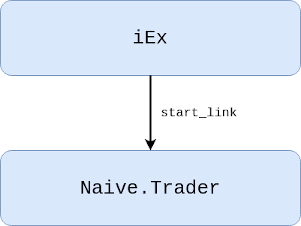
\includegraphics{images/chapter_05_01_current_state.png}

\texttt{GenServer.start\_link/3} creates a link between IEx's process and new \texttt{Naive.Trader} process. Whenever trader terminates(either finishes the trading cycle or there was an error), new one won't get started as there's no supervision at all.

We can do much better than that with a a little bit of help from Elixir and OTP.

Let's introduce a supervisor above our trader process. It will start a new trader process whenever previous one finished/crashed:

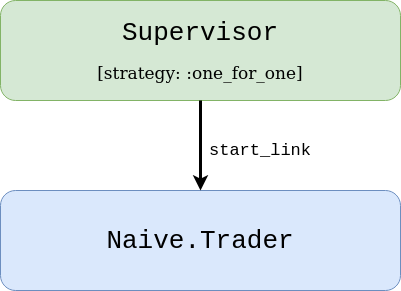
\includegraphics{images/chapter_05_02_supervise_the_trader.png}

This looks much better but there are few problems with it. So, when the trader will start to place orders it will be in \emph{some} state(it will hold buy/sell orders) that the supervisor won't be aware of. In case of trader crashing, the supervisor will start a new trader \emph{without} any knowledge of possibly placed orders or any other information from the state(it will be started with a ``fresh'' state).

To fix that we need to keep a copy of the trader's state outside of the trader process - that's why we will introduce a new server called \texttt{Naive.Leader} that will keep track of traders' data:

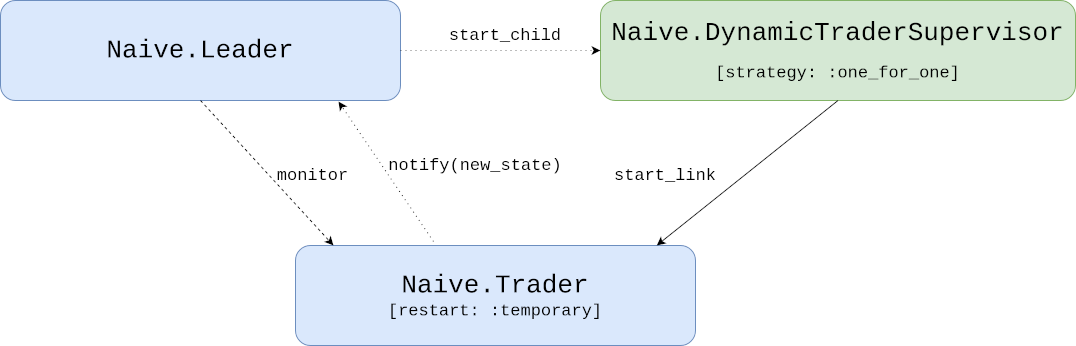
\includegraphics{images/chapter_05_03_leader_added.png}

The \texttt{Naive.Leader} will become the interface to start new \emph{traders}. It will call the \texttt{start\_child/1} function of the Supervisor, then consequently \texttt{DynamicTraderSupervisor} will call the \texttt{start\_link/1} function of our \texttt{Naive.Trader} module.

We can also see that our \texttt{Naive.Trader}'s are now started with the \texttt{temporary\ restart} option. Setting this option will disallow the Supervisor from restarting the traders on its own. The responsibility of restarting traders will now be shifted to the leader. Leader will monitor the traders and restart them to a correct state when any crashes.

As trader state will get updated, it will notify the leader about it's new state to be stored. This way whenever trader would crash, leader will be able to start new trader process with last known state.

This setup will also allow us to start and supervise multiple traders for a single symbol which our naive strategy will require in the future(next chapter).

For each symbol that we will be trading on we need a above trio of services(Leader + DynamicTraderSupervisor + Trader), to effectively initialize(and supervise) them we will add an \texttt{Naive.SymbolSupervisor} that will start both \texttt{Naive.Leader} and `Naive.Dynamic:

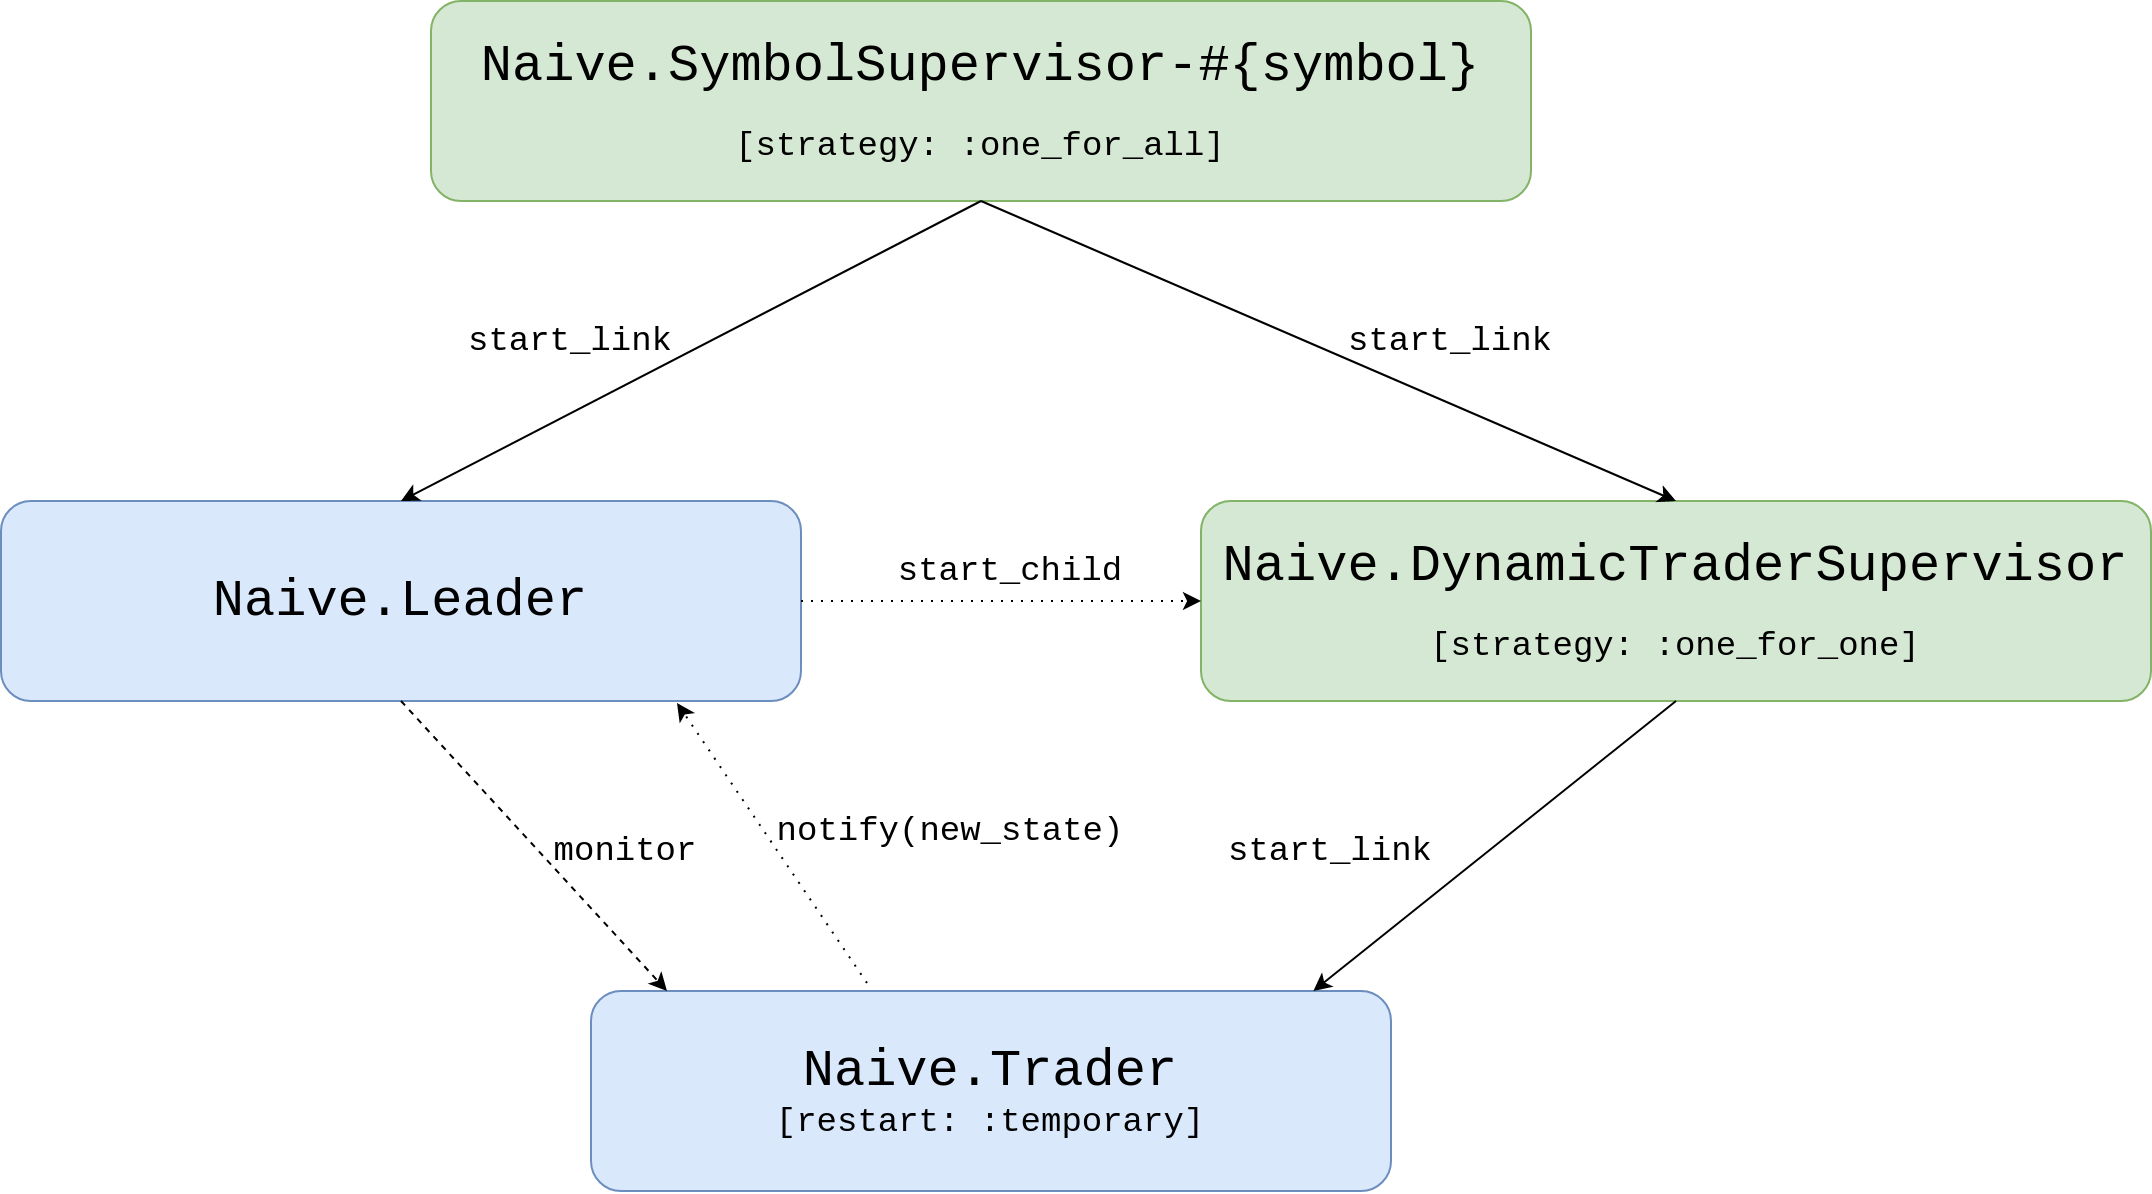
\includegraphics{images/chapter_05_04_symbol_sup.png}

We will need multiple symbol supervisors, one for each symbol that we would like to trade on. As with traders, they will be dynamically started on demand, this should give us a hint that we need another dynamic supervisor that will supervise symbol supervisors and will be direct child of our \texttt{Naive.Supervisor}(\texttt{Naive.Application} module):

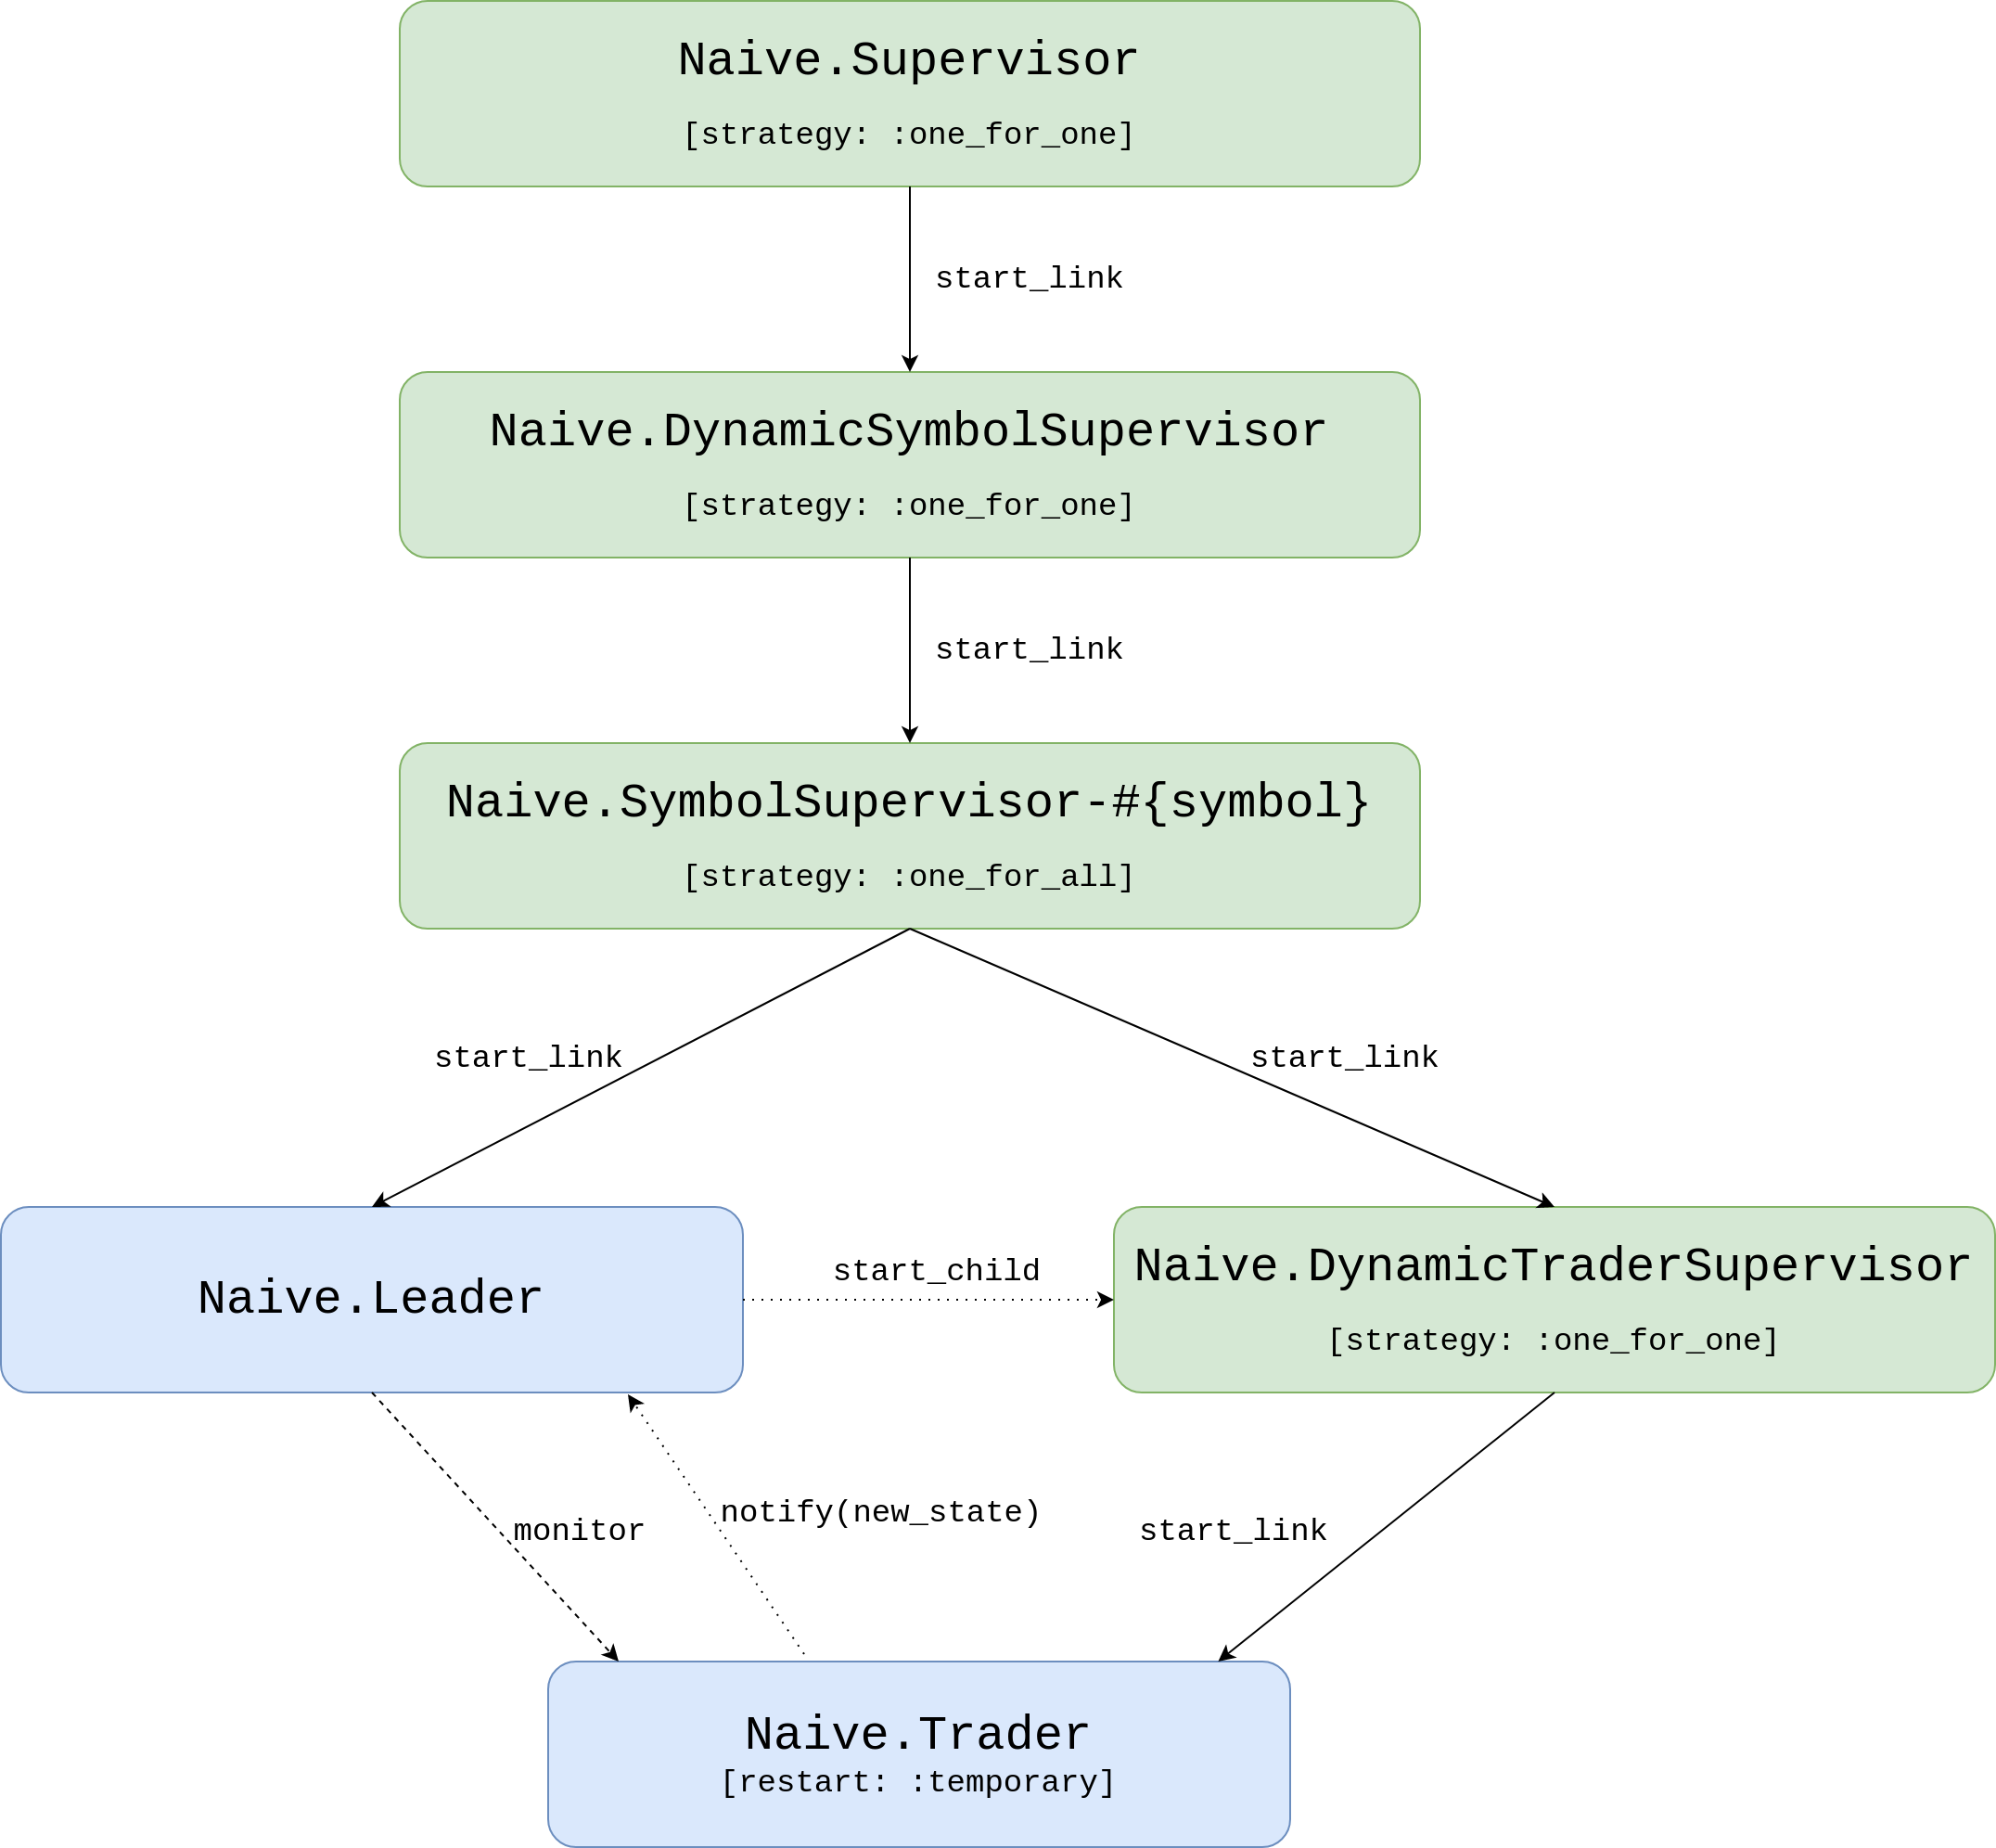
\includegraphics{images/chapter_05_05_full.png}

You could ask yourself why we don't need some additional server to track which symbols are traded at the moment (in the same way as \texttt{Naive.Leader} tracks \texttt{Naive.Trader}s). The answer is that we don't need to track them as we register all \texttt{Naive.SymbolSupervisor}s with a name containing symbol that they trade on. This way we will always be able to refer to them by registered name instead of pids/refs.

Here's what happens starting from the top of the graph:
- the \texttt{Naive.Application} is our top-level application's supervisor for the \texttt{naive} app, it was auto-generated as a part of the \texttt{naive} app
- it has a single child \texttt{Naive.DynamicSymbolSupervisor}, which has strategy one\_for\_one and all of it's children are \texttt{Naive.SymbolSupervisor}s
- \texttt{Naive.SymbolSupervisor} process will start 2 further children: the \texttt{Naive.Leader} and \texttt{DynamicTraderSupervisor}, both created on init
- the \texttt{Naive.Leader} will ask \texttt{DynamicTraderSupervisor} to start the \texttt{Naive.Trader} child process(es)

This can be a little bit confusing at the moment but it will get a lot easier
as we will write the code. Let's get to it!

\hypertarget{update-application-supervisor}{%
\subsection{Update application supervisor}\label{update-application-supervisor}}

Let's start by adding a \texttt{Naive.DynamicSymbolSupervisor} and a server to the children list of the \texttt{Naive.Application} supervisor:

\begin{Shaded}
\begin{Highlighting}[]
  \CommentTok{\# /apps/naive/lib/naive/application.ex}
  \KeywordTok{def}\NormalTok{ start(\_type, \_args) }\KeywordTok{do}
\NormalTok{    children }\OperatorTok{=}\NormalTok{ [}
\NormalTok{      \{}
        \ConstantTok{DynamicSupervisor}\NormalTok{,}
        \VariableTok{strategy:} \VariableTok{:one\_for\_one}\NormalTok{,}
        \VariableTok{name:} \ConstantTok{Naive}\OperatorTok{.}\ConstantTok{DynamicSymbolSupervisor}
\NormalTok{      \}}
\NormalTok{    ]}

    \OperatorTok{...}
  \KeywordTok{end}
\end{Highlighting}
\end{Shaded}

\hypertarget{add-interface-method}{%
\subsection{Add interface method}\label{add-interface-method}}

We will now add an interface method to the \texttt{Naive} module that will instruct \texttt{Naive.DynamicSymbolSupervisor} to start \texttt{Naive.SymbolSupervisor}(to be implemented next) as it's child:

\begin{Shaded}
\begin{Highlighting}[]
  \CommentTok{\# /apps/naive/lib/naive.ex}
  \KeywordTok{def}\NormalTok{ start\_trading(symbol) }\KeywordTok{do}
\NormalTok{    symbol }\OperatorTok{=} \ConstantTok{String}\OperatorTok{.}\NormalTok{upcase(symbol)}

\NormalTok{    \{}\VariableTok{:ok}\NormalTok{, \_pid\} }\OperatorTok{=}
      \ConstantTok{DynamicSupervisor}\OperatorTok{.}\NormalTok{start\_child(}
        \ConstantTok{Naive}\OperatorTok{.}\ConstantTok{DynamicSymbolSupervisor}\NormalTok{,}
\NormalTok{        \{}\ConstantTok{Naive}\OperatorTok{.}\ConstantTok{SymbolSupervisor}\NormalTok{, symbol\}}
\NormalTok{      )}
  \KeywordTok{end}
\end{Highlighting}
\end{Shaded}

\hypertarget{implement-naive.symbolsupervisor}{%
\section{\texorpdfstring{Implement \texttt{Naive.SymbolSupervisor}}{Implement Naive.SymbolSupervisor}}\label{implement-naive.symbolsupervisor}}

Next, time for the \texttt{Naive.SymbolSupervisor}, first step will be to create a file called \texttt{symbol\_supervisor.ex} inside \texttt{apps/naive/lib/naive} directory. There's no point of using the \href{https://hexdocs.pm/elixir/master/DynamicSupervisor.html}{DynamicSupervisor}, as we know the children that we would like to start automatically on init. This is a full implementation of the supervisor and it's a simple as just listing child processes inside the init function:

\begin{Shaded}
\begin{Highlighting}[]
\CommentTok{\# /apps/naive/lib/naive/symbol\_supervisor.ex}
\KeywordTok{defmodule} \ConstantTok{Naive}\OperatorTok{.}\ConstantTok{SymbolSupervisor} \KeywordTok{do}
  \ImportTok{use} \ConstantTok{Supervisor}

  \ImportTok{require} \ConstantTok{Logger}

  \KeywordTok{def}\NormalTok{ start\_link(symbol) }\KeywordTok{do}
    \ConstantTok{Supervisor}\OperatorTok{.}\NormalTok{start\_link(}
      \ConstantTok{\_\_MODULE\_\_}\NormalTok{,}
\NormalTok{      symbol,}
      \VariableTok{name:}\NormalTok{ :}\StringTok{"}\OtherTok{\#\{}\ConstantTok{\_\_MODULE\_\_}\OtherTok{\}}\StringTok{{-}}\OtherTok{\#\{}\NormalTok{symbol}\OtherTok{\}}\StringTok{"}
\NormalTok{    )}
  \KeywordTok{end}

  \KeywordTok{def}\NormalTok{ init(symbol) }\KeywordTok{do}
    \ConstantTok{Logger}\OperatorTok{.}\NormalTok{info(}\StringTok{"Starting new supervision tree to trade on }\OtherTok{\#\{}\NormalTok{symbol}\OtherTok{\}}\StringTok{"}\NormalTok{)}

    \ConstantTok{Supervisor}\OperatorTok{.}\NormalTok{init(}
\NormalTok{      [}
\NormalTok{        \{}
          \ConstantTok{DynamicSupervisor}\NormalTok{,}
          \VariableTok{strategy:} \VariableTok{:one\_for\_one}\NormalTok{,}
          \VariableTok{name:}\NormalTok{ :}\StringTok{"Naive.DynamicTraderSupervisor{-}}\OtherTok{\#\{}\NormalTok{symbol}\OtherTok{\}}\StringTok{"}
\NormalTok{        \},}
\NormalTok{        \{}\ConstantTok{Naive}\OperatorTok{.}\ConstantTok{Leader}\NormalTok{, symbol\}}
\NormalTok{      ],}
      \VariableTok{strategy:} \VariableTok{:one\_for\_all}
\NormalTok{    )}
  \KeywordTok{end}
\KeywordTok{end}
\end{Highlighting}
\end{Shaded}

It's advised to keep supervisor processes slim.

We registered the \texttt{Naive.SymbolSupervisor} processes with names, which will help us understand the supervision tree inside the observer GUI(it will also allow us to stop those supervisors in the future).

As mentioned previously whenever either the \texttt{Naive.Leader} or \texttt{Naive.DynamicSymbolSupervisor-\#\{symbol\}} would crash we would like to kill the other child process as we won't be able to recover the state - it's just easier to init both again.

\hypertarget{implement-naive.leader}{%
\section{\texorpdfstring{Implement \texttt{Naive.Leader}}{Implement Naive.Leader}}\label{implement-naive.leader}}

It's time for the \texttt{Naive.Leader} module, again, first step will be to create a file called \texttt{leader.ex} inside \texttt{apps/naive/lib/naive} directory. At this moment it will be a skeleton GenServer implementation just to get the code to compile:

\begin{Shaded}
\begin{Highlighting}[]
\CommentTok{\# /apps/naive/lib/naive/leader.ex}
\KeywordTok{defmodule} \ConstantTok{Naive}\OperatorTok{.}\ConstantTok{Leader} \KeywordTok{do}
  \ImportTok{use} \ConstantTok{GenServer}

  \KeywordTok{def}\NormalTok{ start\_link(symbol) }\KeywordTok{do}
    \ConstantTok{GenServer}\OperatorTok{.}\NormalTok{start\_link(}
      \ConstantTok{\_\_MODULE\_\_}\NormalTok{,}
\NormalTok{      symbol,}
      \VariableTok{name:}\NormalTok{ :}\StringTok{"}\OtherTok{\#\{}\ConstantTok{\_\_MODULE\_\_}\OtherTok{\}}\StringTok{{-}}\OtherTok{\#\{}\NormalTok{symbol}\OtherTok{\}}\StringTok{"}
\NormalTok{    )}
  \KeywordTok{end}

  \KeywordTok{def}\NormalTok{ init(symbol) }\KeywordTok{do}
\NormalTok{    \{}\VariableTok{:ok}\NormalTok{, \%\{}\VariableTok{symbol:}\NormalTok{ symbol\}\}}
  \KeywordTok{end}
\KeywordTok{end}
\end{Highlighting}
\end{Shaded}

At this moment we have half of the supervision tree working so we can give it
a spin in iex. Using the observer we will be able to see all processes created when start trading function gets called:

\begin{Shaded}
\begin{Highlighting}[]
\ExtensionTok{$}\NormalTok{ iex }\AttributeTok{{-}S}\NormalTok{ mix}
\ExtensionTok{...}
\ExtensionTok{iex}\ErrorTok{(}\ExtensionTok{1}\KeywordTok{)}\OperatorTok{\textgreater{}}\NormalTok{ :observer.start}\KeywordTok{()}
\end{Highlighting}
\end{Shaded}

Above function will open a new window looking as follows:

\begin{figure}
\centering
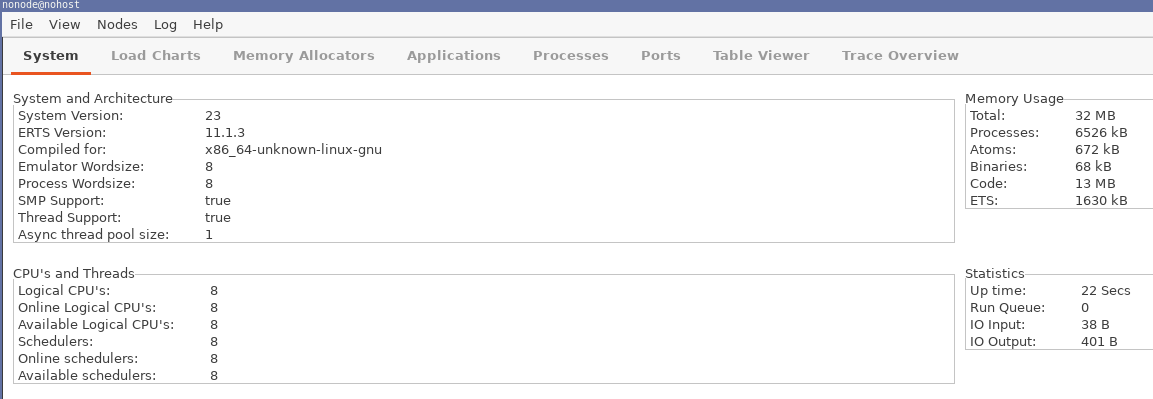
\includegraphics{images/chapter_05_06_new_observer.png}
\caption{New observer window}
\end{figure}

To clearly see the supervision tree we will click on ``Applications'' tab at the top - the following tree of processes will be shown on the left:

\begin{figure}
\centering
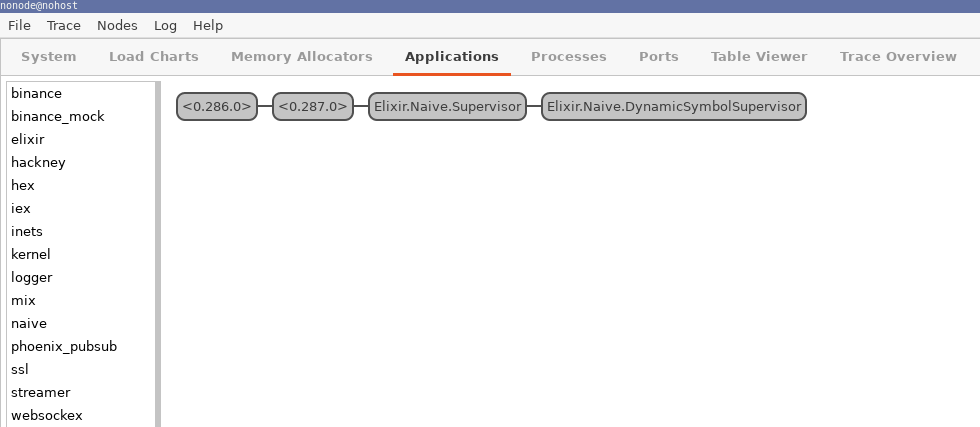
\includegraphics{images/chapter_05_07_observer_app_list.png}
\caption{Observer applications list}
\end{figure}

If any other process tree is visible, go to the list on the left and select the \texttt{naive} application.

The \texttt{Naive.Supervisor} is our \texttt{Naive.Application} module(you can confirm that by checking the \texttt{name} option send to the \texttt{start\_link} function inside the module). It start the \texttt{Naive.DynamicSymbolSupervisor}.

We can now call the \texttt{Naive.start\_trading/1} function couple time to see how the tree will look like with additional processes(go back to the \texttt{iex} session):

\begin{Shaded}
\begin{Highlighting}[]
\ExtensionTok{...}
\ExtensionTok{iex}\ErrorTok{(}\ExtensionTok{2}\KeywordTok{)}\OperatorTok{\textgreater{}}\NormalTok{ Naive.start\_trading}\KeywordTok{(}\StringTok{"adausdt"}\KeywordTok{)}
\ExtensionTok{23:14:40.974}\NormalTok{ [info]  Starting new supervision tree to trade on ADAUSDT}
\ExtensionTok{\{:ok,} \CommentTok{\#PID\textless{}0.340.0\textgreater{}\}}
\ExtensionTok{iex}\ErrorTok{(}\ExtensionTok{3}\KeywordTok{)}\OperatorTok{\textgreater{}}\NormalTok{ Naive.start\_trading}\KeywordTok{(}\StringTok{"xrpusdt"}\KeywordTok{)}
\ExtensionTok{23:15:12.117}\NormalTok{ [info]  Starting new supervision tree to trade on XRPUSDT}
\ExtensionTok{\{:ok,} \CommentTok{\#PID\textless{}0.345.0\textgreater{}\}}
\end{Highlighting}
\end{Shaded}

We can see that two new branches were created:
- \texttt{SymbolSupervisor-ADAUSDT}
- \texttt{SymbolSupervisor-XRPUSDT}

Each of them contain a \texttt{Naive.Leader} and \texttt{DynamicTraderSupervisor}.

\hypertarget{updating-the-leader-module}{%
\subsection{\texorpdfstring{Updating the \texttt{leader} module}{Updating the leader module}}\label{updating-the-leader-module}}

Let's jump back to extending a leader implementation to get those traders running.

We will introduce a leader's state that will consist of symbol, setting and a list of traders' data. Trader data will hold pid, ref and state of the trader:

\begin{Shaded}
\begin{Highlighting}[]
\CommentTok{\# /apps/naive/lib/naive/leader.ex}
  \OperatorTok{...}
  \ImportTok{alias} \ConstantTok{Naive}\OperatorTok{.}\ConstantTok{Trader}

  \ImportTok{require} \ConstantTok{Logger}

  \OtherTok{@binance\_client} \ConstantTok{Application}\OperatorTok{.}\NormalTok{get\_env(}\VariableTok{:naive}\NormalTok{, }\VariableTok{:binance\_client}\NormalTok{)}

  \KeywordTok{defmodule} \ConstantTok{State} \KeywordTok{do}
    \KeywordTok{defstruct} \VariableTok{symbol:} \ConstantTok{nil}\NormalTok{,}
              \VariableTok{settings:} \ConstantTok{nil}\NormalTok{,}
              \VariableTok{traders:}\NormalTok{ []}
  \KeywordTok{end}

  \KeywordTok{defmodule} \ConstantTok{TraderData} \KeywordTok{do}
    \KeywordTok{defstruct} \VariableTok{pid:} \ConstantTok{nil}\NormalTok{,}
              \VariableTok{ref:} \ConstantTok{nil}\NormalTok{,}
              \VariableTok{state:} \ConstantTok{nil}
  \KeywordTok{end}
\end{Highlighting}
\end{Shaded}

We will use a \texttt{handle\_continue} callback which was introduced in Erlang 21 to
initialize the leader asynchronously. To do that we will return a tuple starting with a \texttt{:continue} atom from inside the init function:

\begin{Shaded}
\begin{Highlighting}[]
  \CommentTok{\# /apps/naive/lib/naive/leader.ex}
  \KeywordTok{def}\NormalTok{ init(symbol) }\KeywordTok{do}
\NormalTok{    \{}\VariableTok{:ok}\NormalTok{,}
\NormalTok{      \%}\ConstantTok{State}\NormalTok{\{}
          \VariableTok{symbol:}\NormalTok{ symbol}
\NormalTok{      \}, \{}\VariableTok{:continue}\NormalTok{, }\VariableTok{:start\_traders}\NormalTok{\}\}}
  \KeywordTok{end}
\end{Highlighting}
\end{Shaded}

The \texttt{Naive.Leader} will fetch symbol settings and based on them, it will build the state for traders so they don't need to fetch the same settings again. It will also start as many traders there were set under chunks key in setting:

\begin{Shaded}
\begin{Highlighting}[]
  \CommentTok{\# /apps/naive/lib/naive/leader.ex}
  \CommentTok{\# below init()}
  \KeywordTok{def}\NormalTok{ handle\_continue(}\VariableTok{:start\_traders}\NormalTok{, \%\{}\VariableTok{symbol:}\NormalTok{ symbol\} }\OperatorTok{=}\NormalTok{ state) }\KeywordTok{do}
\NormalTok{    settings }\OperatorTok{=}\NormalTok{ fetch\_symbol\_settings(symbol)}
\NormalTok{    trader\_state }\OperatorTok{=}\NormalTok{ fresh\_trader\_state(settings)}
\NormalTok{    traders }\OperatorTok{=} \KeywordTok{for}\NormalTok{ \_i }\OperatorTok{\textless{}{-}} \DecValTok{1}\OperatorTok{..}\NormalTok{settings}\OperatorTok{.}\NormalTok{chunks,}
              \KeywordTok{do}\NormalTok{: start\_new\_trader(trader\_state)}

\NormalTok{    \{}\VariableTok{:noreply}\NormalTok{, \%\{state }\OperatorTok{|} \VariableTok{settings:}\NormalTok{ settings, }\VariableTok{traders:}\NormalTok{ traders\}\}}
  \KeywordTok{end}
\end{Highlighting}
\end{Shaded}

Fetching symbol settings will be hardcoded for time being to keep this chapter focused. We will also move the code responsible for fetching tick
size from the \texttt{Naive.Trader} to the \texttt{Naive.Leader} and hardcode the rest of the values:

\begin{Shaded}
\begin{Highlighting}[]
  \CommentTok{\# /apps/naive/lib/naive/leader.ex}
  \KeywordTok{defp}\NormalTok{ fetch\_symbol\_settings(symbol) }\KeywordTok{do}
\NormalTok{    tick\_size }\OperatorTok{=}\NormalTok{ fetch\_tick\_size(symbol)}

\NormalTok{    \%\{}
      \VariableTok{symbol:}\NormalTok{ symbol,}
      \VariableTok{chunks:} \DecValTok{1}\NormalTok{,}
      \CommentTok{\# {-}0.12\% for quick testing}
      \VariableTok{profit\_interval:} \ConstantTok{Decimal}\OperatorTok{.}\NormalTok{new(}\StringTok{"{-}0.0012"}\NormalTok{),}
      \VariableTok{tick\_size:}\NormalTok{ tick\_size}
\NormalTok{    \}}
  \KeywordTok{end}

  \KeywordTok{defp}\NormalTok{ fetch\_tick\_size(symbol) }\KeywordTok{do}
    \OtherTok{@binance\_client}\OperatorTok{.}\NormalTok{get\_exchange\_info()}
    \OperatorTok{|\textgreater{}}\NormalTok{ elem(}\DecValTok{1}\NormalTok{)}
    \OperatorTok{|\textgreater{}} \ConstantTok{Map}\OperatorTok{.}\NormalTok{get(}\VariableTok{:symbols}\NormalTok{)}
    \OperatorTok{|\textgreater{}} \ConstantTok{Enum}\OperatorTok{.}\NormalTok{find(}\OperatorTok{\&}\NormalTok{(}\OperatorTok{\&}\DecValTok{1}\NormalTok{[}\StringTok{"symbol"}\NormalTok{] }\OperatorTok{==}\NormalTok{ symbol))}
    \OperatorTok{|\textgreater{}} \ConstantTok{Map}\OperatorTok{.}\NormalTok{get(}\StringTok{"filters"}\NormalTok{)}
    \OperatorTok{|\textgreater{}} \ConstantTok{Enum}\OperatorTok{.}\NormalTok{find(}\OperatorTok{\&}\NormalTok{(}\OperatorTok{\&}\DecValTok{1}\NormalTok{[}\StringTok{"filterType"}\NormalTok{] }\OperatorTok{==} \StringTok{"PRICE\_FILTER"}\NormalTok{))}
    \OperatorTok{|\textgreater{}} \ConstantTok{Map}\OperatorTok{.}\NormalTok{get(}\StringTok{"tickSize"}\NormalTok{)}
    \OperatorTok{|\textgreater{}} \ConstantTok{Decimal}\OperatorTok{.}\NormalTok{new()}
  \KeywordTok{end}
\end{Highlighting}
\end{Shaded}

Additionally we need to create a helper method that we used inside the \texttt{handle\_continue/2} callback called \texttt{fresh\_trader\_state/1}:

\begin{Shaded}
\begin{Highlighting}[]
  \CommentTok{\# /apps/naive/lib/naive/leader.ex}
  \CommentTok{\# place this one above the \textasciigrave{}fetch\_symbol\_settings\textasciigrave{} function}
  \KeywordTok{defp}\NormalTok{ fresh\_trader\_state(settings) }\KeywordTok{do}
\NormalTok{    struct(}\ConstantTok{Trader}\OperatorTok{.}\ConstantTok{State}\NormalTok{, settings)}
  \KeywordTok{end}
\end{Highlighting}
\end{Shaded}

Starting a new trader isn't any different from the code that we already wrote to start a new \texttt{Naive.SymbolSupervisor}. We need to call the \texttt{DynamicSupervisor.start\_child/2} function and start to monitor the process:

\begin{Shaded}
\begin{Highlighting}[]
  \CommentTok{\# /apps/naive/lib/naive/leader.ex}
  \KeywordTok{defp}\NormalTok{ start\_new\_trader(\%}\ConstantTok{Trader}\OperatorTok{.}\ConstantTok{State}\NormalTok{\{\} }\OperatorTok{=}\NormalTok{ state) }\KeywordTok{do}
\NormalTok{    \{}\VariableTok{:ok}\NormalTok{, pid\} }\OperatorTok{=}
      \ConstantTok{DynamicSupervisor}\OperatorTok{.}\NormalTok{start\_child(}
\NormalTok{        :}\StringTok{"Naive.DynamicTraderSupervisor{-}}\OtherTok{\#\{}\NormalTok{state}\OperatorTok{.}\NormalTok{symbol}\OtherTok{\}}\StringTok{"}\NormalTok{,}
\NormalTok{        \{}\ConstantTok{Naive}\OperatorTok{.}\ConstantTok{Trader}\NormalTok{, state\}}
\NormalTok{      )}

\NormalTok{    ref }\OperatorTok{=} \ConstantTok{Process}\OperatorTok{.}\NormalTok{monitor(pid)}

\NormalTok{    \%}\ConstantTok{TraderData}\NormalTok{\{}\VariableTok{pid:}\NormalTok{ pid, }\VariableTok{ref:}\NormalTok{ ref, }\VariableTok{state:}\NormalTok{ state\}}
  \KeywordTok{end}
\end{Highlighting}
\end{Shaded}

\hypertarget{updating-the-naive.trader-module}{%
\subsection{\texorpdfstring{Updating the \texttt{Naive.Trader} module}{Updating the Naive.Trader module}}\label{updating-the-naive.trader-module}}

Now we can update the \texttt{Naive.Trader}, first, we will set restart to be temporary to avoid restarting it by the \texttt{Naive.DynamicTraderSupervisor}:

\begin{Shaded}
\begin{Highlighting}[]
\CommentTok{\# /apps/naive/lib/naive/trader.ex}
\KeywordTok{defmodule} \ConstantTok{Naive}\OperatorTok{.}\ConstantTok{Trader} \KeywordTok{do}
  \ImportTok{use} \ConstantTok{GenServer}\NormalTok{, }\VariableTok{restart:} \VariableTok{:temporary}
  \OperatorTok{...}
\end{Highlighting}
\end{Shaded}

Next, we will update \texttt{start\_link/1} and \texttt{init/1} to take the state instead of building it from args:

\begin{Shaded}
\begin{Highlighting}[]
  \CommentTok{\# /apps/naive/lib/naive/trader.ex}
  \KeywordTok{def}\NormalTok{ start\_link(\%}\ConstantTok{State}\NormalTok{\{\} }\OperatorTok{=}\NormalTok{ state) }\KeywordTok{do}
    \ConstantTok{GenServer}\OperatorTok{.}\NormalTok{start\_link(}\ConstantTok{\_\_MODULE\_\_}\NormalTok{, state)}
  \KeywordTok{end}

  \KeywordTok{def}\NormalTok{ init(\%}\ConstantTok{State}\NormalTok{\{}\VariableTok{symbol:}\NormalTok{ symbol\} }\OperatorTok{=}\NormalTok{ state) }\KeywordTok{do}
\NormalTok{    symbol }\OperatorTok{=} \ConstantTok{String}\OperatorTok{.}\NormalTok{upcase(symbol)}

    \ConstantTok{Logger}\OperatorTok{.}\NormalTok{info(}\StringTok{"Initializing new trader for symbol(}\OtherTok{\#\{}\NormalTok{symbol}\OtherTok{\}}\StringTok{)"}\NormalTok{)}

    \ConstantTok{Phoenix}\OperatorTok{.}\ConstantTok{PubSub}\OperatorTok{.}\NormalTok{subscribe(}
      \ConstantTok{Streamer}\OperatorTok{.}\ConstantTok{PubSub}\NormalTok{,}
      \StringTok{"TRADE\_EVENTS:}\OtherTok{\#\{}\NormalTok{symbol}\OtherTok{\}}\StringTok{"}
\NormalTok{    )}

\NormalTok{    \{}\VariableTok{:ok}\NormalTok{, state\}}
  \KeywordTok{end}
\end{Highlighting}
\end{Shaded}

Next, we need to update two \texttt{handle\_info/2} callbacks that change the state of the \texttt{Naive.Trader} process(when placing buy order and when placing sell order). They will need to notify the \texttt{Naive.Leader} that state is changed before returning it:

\begin{Shaded}
\begin{Highlighting}[]
  \CommentTok{\# /apps/naive/lib/naive/trader.ex}
  \OperatorTok{...}

  \KeywordTok{def}\NormalTok{ handle\_info(}
        \OperatorTok{...}
\NormalTok{      ) }\KeywordTok{do}
    \ConstantTok{Logger}\OperatorTok{.}\NormalTok{info(}\StringTok{"Placing buy order (}\OtherTok{\#\{}\NormalTok{symbol}\OtherTok{\}}\StringTok{@}\OtherTok{\#\{}\NormalTok{price}\OtherTok{\}}\StringTok{)"}\NormalTok{)}
    \OperatorTok{...}
\NormalTok{    new\_state }\OperatorTok{=}\NormalTok{ \%\{state }\OperatorTok{|} \VariableTok{buy\_order:}\NormalTok{ order\}}
    \ConstantTok{Naive}\OperatorTok{.}\ConstantTok{Leader}\OperatorTok{.}\NormalTok{notify(}\VariableTok{:trader\_state\_updated}\NormalTok{, new\_state)}
\NormalTok{    \{}\VariableTok{:noreply}\NormalTok{, new\_state\}}
  \KeywordTok{end}

  \KeywordTok{def}\NormalTok{ handle\_info(}
        \OperatorTok{...}
\NormalTok{      ) }\KeywordTok{do}
    \OperatorTok{...}
    \ConstantTok{Logger}\OperatorTok{.}\NormalTok{info(}\StringTok{"Buy order filled, placing sell order ..."}\NormalTok{)  }
    \OperatorTok{...}

\NormalTok{    new\_state }\OperatorTok{=}\NormalTok{ \%\{state }\OperatorTok{|} \VariableTok{sell\_order:}\NormalTok{ order\}}
    \ConstantTok{Naive}\OperatorTok{.}\ConstantTok{Leader}\OperatorTok{.}\NormalTok{notify(}\VariableTok{:trader\_state\_updated}\NormalTok{, new\_state)}
\NormalTok{    \{}\VariableTok{:noreply}\NormalTok{, new\_state\}}
  \KeywordTok{end}
  \OperatorTok{...}
\end{Highlighting}
\end{Shaded}

\hypertarget{finalizing-naive.leader-implementation}{%
\subsection{\texorpdfstring{Finalizing \texttt{Naive.Leader} implementation}{Finalizing Naive.Leader implementation}}\label{finalizing-naive.leader-implementation}}

Now we need to get back to the \texttt{Naive.Leader} where we will implement the notifing logic. We will start with the notify function that will just call the \texttt{Naive.Leader} process:

\begin{Shaded}
\begin{Highlighting}[]
  \CommentTok{\# /apps/naive/lib/naive/leader.ex}
  \CommentTok{\# below init}

  \KeywordTok{def}\NormalTok{ notify(}\VariableTok{:trader\_state\_updated}\NormalTok{, trader\_state) }\KeywordTok{do}
    \ConstantTok{GenServer}\OperatorTok{.}\NormalTok{call(}
\NormalTok{      :}\StringTok{"}\OtherTok{\#\{}\ConstantTok{\_\_MODULE\_\_}\OtherTok{\}}\StringTok{{-}}\OtherTok{\#\{}\NormalTok{trader\_state}\OperatorTok{.}\NormalTok{symbol}\OtherTok{\}}\StringTok{"}\NormalTok{,}
\NormalTok{      \{}\VariableTok{:update\_trader\_state}\NormalTok{, trader\_state\}}
\NormalTok{    )}
  \KeywordTok{end}
\end{Highlighting}
\end{Shaded}

Now, it's time for a callback function that will handle the trader state update. As this is a \texttt{handle\_call/3} callback we have access to trader pid which sent the notification message. We will try to find that trader in the list of traders. If that's successful we will update the cached state for that
trader locally:

\begin{Shaded}
\begin{Highlighting}[]
  \CommentTok{\# /apps/naive/lib/naive/leader.ex}
  \CommentTok{\# below handle\_continue}
  \KeywordTok{def}\NormalTok{ handle\_call(}
\NormalTok{    \{}\VariableTok{:update\_trader\_state}\NormalTok{, new\_trader\_state\},}
\NormalTok{    \{trader\_pid, \_\},}
\NormalTok{    \%\{}\VariableTok{traders:}\NormalTok{ traders\} }\OperatorTok{=}\NormalTok{ state}
\NormalTok{  ) }\KeywordTok{do}
    \KeywordTok{case} \ConstantTok{Enum}\OperatorTok{.}\NormalTok{find\_index(traders, }\OperatorTok{\&}\NormalTok{(}\OperatorTok{\&}\DecValTok{1}\OperatorTok{.}\NormalTok{pid }\OperatorTok{==}\NormalTok{ trader\_pid)) }\KeywordTok{do}
      \ConstantTok{nil} \OperatorTok{{-}\textgreater{}}
        \ConstantTok{Logger}\OperatorTok{.}\NormalTok{warn(}
          \StringTok{"Tried to update the state of trader that leader is not aware of"}
\NormalTok{        )}
\NormalTok{        \{}\VariableTok{:reply}\NormalTok{, }\VariableTok{:ok}\NormalTok{, state\}}
      
\NormalTok{      index }\OperatorTok{{-}\textgreater{}}
\NormalTok{        old\_trader\_data }\OperatorTok{=} \ConstantTok{Enum}\OperatorTok{.}\NormalTok{at(traders, index)}
\NormalTok{        new\_trader\_data }\OperatorTok{=}\NormalTok{ \%\{old\_trader\_data }\OperatorTok{|} \VariableTok{:state} \OperatorTok{=\textgreater{}}\NormalTok{ new\_trader\_state\}}

\NormalTok{        \{}\VariableTok{:reply}\NormalTok{, }\VariableTok{:ok}\NormalTok{, \%\{state }\OperatorTok{|} \VariableTok{:traders} \OperatorTok{=\textgreater{}}
          \ConstantTok{List}\OperatorTok{.}\NormalTok{replace\_at(traders, index, new\_trader\_data)\}\}}
    \KeywordTok{end}
  \KeywordTok{end}
\end{Highlighting}
\end{Shaded}

Another callback functions that we will need to provide are two \texttt{handle\_info/2} functions that will handle the trade finished scenario as well as crashed trader.

First, trade finished scenario. As previously, we will try to find the trader data in the traders list. If that's successful, we will start a new trader with fresh state. We will also overwrite existing trader data locally(as pid, ref and state changed):

\begin{Shaded}
\begin{Highlighting}[]
  \CommentTok{\# /apps/naive/lib/naive/leader.ex}
  \CommentTok{\# below state updated handle\_call callback}
  \KeywordTok{def}\NormalTok{ handle\_info(}
\NormalTok{        \{}\VariableTok{:DOWN}\NormalTok{, \_ref, }\VariableTok{:process}\NormalTok{, trader\_pid, }\VariableTok{:normal}\NormalTok{\},}
\NormalTok{        \%\{}\VariableTok{traders:}\NormalTok{ traders, }\VariableTok{symbol:}\NormalTok{ symbol, }\VariableTok{settings:}\NormalTok{ settings\} }\OperatorTok{=}\NormalTok{ state}
\NormalTok{      ) }\KeywordTok{do}
    \ConstantTok{Logger}\OperatorTok{.}\NormalTok{info(}\StringTok{"}\OtherTok{\#\{}\NormalTok{symbol}\OtherTok{\}}\StringTok{ trader finished trade {-} restarting"}\NormalTok{)}

    \KeywordTok{case} \ConstantTok{Enum}\OperatorTok{.}\NormalTok{find\_index(traders, }\OperatorTok{\&}\NormalTok{(}\OperatorTok{\&}\DecValTok{1}\OperatorTok{.}\NormalTok{pid }\OperatorTok{==}\NormalTok{ trader\_pid)) }\KeywordTok{do}
      \ConstantTok{nil} \OperatorTok{{-}\textgreater{}}
        \ConstantTok{Logger}\OperatorTok{.}\NormalTok{warn(}
          \StringTok{"Tried to restart finished }\OtherTok{\#\{}\NormalTok{symbol}\OtherTok{\}}\StringTok{ "} \OperatorTok{\textless{}\textgreater{}}
            \StringTok{"trader that leader is not aware of"}
\NormalTok{        )}

\NormalTok{        \{}\VariableTok{:noreply}\NormalTok{, state\}}

\NormalTok{      index }\OperatorTok{{-}\textgreater{}}
\NormalTok{        new\_trader\_data }\OperatorTok{=}\NormalTok{ start\_new\_trader(fresh\_trader\_state(settings))}
\NormalTok{        new\_traders }\OperatorTok{=} \ConstantTok{List}\OperatorTok{.}\NormalTok{replace\_at(traders, index, new\_trader\_data)}

\NormalTok{        \{}\VariableTok{:noreply}\NormalTok{, \%\{state }\OperatorTok{|} \VariableTok{traders:}\NormalTok{ new\_traders\}\}}
    \KeywordTok{end}
  \KeywordTok{end}
\end{Highlighting}
\end{Shaded}

Here we will assume that whenever the reason that the \texttt{Naive.Trader} process died is \texttt{:normal} that means that we stopped it after trade cycle finished.

Final callback that we need to provide will handle the scenario where the trader crashed. We would like to find the cached state of the crashed trader and start a new one with the same state and then update the local cache as pid and ref will change for that trader:

\begin{Shaded}
\begin{Highlighting}[]
  \CommentTok{\# /apps/naive/lib/naive/leader.ex}
  \CommentTok{\# below trade finished handle\_info callback}
  \KeywordTok{def}\NormalTok{ handle\_info(}
\NormalTok{        \{}\VariableTok{:DOWN}\NormalTok{, \_ref, }\VariableTok{:process}\NormalTok{, trader\_pid, \_reason\},}
\NormalTok{        \%\{}\VariableTok{traders:}\NormalTok{ traders, }\VariableTok{symbol:}\NormalTok{ symbol\} }\OperatorTok{=}\NormalTok{ state}
\NormalTok{      ) }\KeywordTok{do}
    \ConstantTok{Logger}\OperatorTok{.}\NormalTok{error(}\StringTok{"}\OtherTok{\#\{}\NormalTok{symbol}\OtherTok{\}}\StringTok{ trader died {-} trying to restart"}\NormalTok{)}

    \KeywordTok{case} \ConstantTok{Enum}\OperatorTok{.}\NormalTok{find\_index(traders, }\OperatorTok{\&}\NormalTok{(}\OperatorTok{\&}\DecValTok{1}\OperatorTok{.}\NormalTok{pid }\OperatorTok{==}\NormalTok{ trader\_pid)) }\KeywordTok{do}
      \ConstantTok{nil} \OperatorTok{{-}\textgreater{}}
        \ConstantTok{Logger}\OperatorTok{.}\NormalTok{warn(}
          \StringTok{"Tried to restart }\OtherTok{\#\{}\NormalTok{symbol}\OtherTok{\}}\StringTok{ trader "} \OperatorTok{\textless{}\textgreater{}}
            \StringTok{"but failed to find its cached state"}
\NormalTok{        )}

\NormalTok{        \{}\VariableTok{:noreply}\NormalTok{, state\}}

\NormalTok{      index }\OperatorTok{{-}\textgreater{}}
\NormalTok{        trader\_data }\OperatorTok{=} \ConstantTok{Enum}\OperatorTok{.}\NormalTok{at(traders, index)}
\NormalTok{        new\_trader\_data }\OperatorTok{=}\NormalTok{ start\_new\_trader(trader\_data}\OperatorTok{.}\NormalTok{state)}
\NormalTok{        new\_traders }\OperatorTok{=} \ConstantTok{List}\OperatorTok{.}\NormalTok{replace\_at(traders, index, new\_trader\_data)}

\NormalTok{        \{}\VariableTok{:noreply}\NormalTok{, \%\{state }\OperatorTok{|} \VariableTok{traders:}\NormalTok{ new\_traders\}\}}
    \KeywordTok{end}
  \KeywordTok{end}
\end{Highlighting}
\end{Shaded}

\hypertarget{iex-testing}{%
\subsection{IEx testing}\label{iex-testing}}

That finishes the implementation part, let's jump into iex session to see how it works.

We will start the observer first, then we will start trading on any valid symbol.

When our trader will start, you should be able to right click and select ``Kill process''(leave the reason as kill) and click ``OK''. At that moment you should see that the PID of the trader changed and we can also see log message from the leader.

\begin{Shaded}
\begin{Highlighting}[]
\ExtensionTok{$}\NormalTok{ iex }\AttributeTok{{-}S}\NormalTok{ mix}
\ExtensionTok{...}
\ExtensionTok{iex}\ErrorTok{(}\ExtensionTok{1}\KeywordTok{)}\OperatorTok{\textgreater{}}\NormalTok{ :observer.start}\KeywordTok{()}             
\ExtensionTok{:ok}
\ExtensionTok{iex}\ErrorTok{(}\ExtensionTok{2}\KeywordTok{)}\OperatorTok{\textgreater{}}\NormalTok{ Naive.start\_trading}\KeywordTok{(}\StringTok{"xrpusdt"}\KeywordTok{)}

\ExtensionTok{00:04:35.041}\NormalTok{ [info]  Starting new supervision tree to trade on XRPUSDT}
\ExtensionTok{\{:ok,} \CommentTok{\#PID\textless{}0.455.0\textgreater{}\}}
\ExtensionTok{00:04:37.697}\NormalTok{ [info]  Initializing new trader for XRPUSDT}
\ExtensionTok{iex}\ErrorTok{(}\ExtensionTok{3}\KeywordTok{)}\OperatorTok{\textgreater{}}
\ExtensionTok{00:08:01.476}\NormalTok{ [error] XRPUSDT trader died }\AttributeTok{{-}}\NormalTok{ trying to restart}
\ExtensionTok{00:08:01.476}\NormalTok{ [info]  Initializing new trader for XRPUSDT}
\end{Highlighting}
\end{Shaded}

{[}Note{]} Please remember to run \texttt{mix\ format} to keep things nice and tidy.

Source code for this chapter can be found at \href{https://github.com/frathon/create-a-cryptocurrency-trading-bot-in-elixir-source-code/tree/chapter_05}{Github}

\hypertarget{introduce-a-buy_down_interval-to-make-a-single-trader-more-profitable}{%
\chapter{\texorpdfstring{Introduce a \texttt{buy\_down\_interval} to make a single trader more profitable}{Introduce a buy\_down\_interval to make a single trader more profitable}}\label{introduce-a-buy_down_interval-to-make-a-single-trader-more-profitable}}

\hypertarget{objectives-5}{%
\section{Objectives}\label{objectives-5}}

\begin{itemize}
\tightlist
\item
  present reasons why to introduce \texttt{buy\_down\_interval}
\item
  add \texttt{buy\_down\ interval} to \texttt{Naive.Trader}'s state and calculate buy price
\item
  add \texttt{buy\_down\ interval} to \texttt{Naive.Trader}'s state compiled by the \texttt{Naive.Leader}
\item
  manually test the implementation inside iex
\end{itemize}

\hypertarget{why-we-need-to-buy-below-the-current-price-feature-overview}{%
\section{Why we need to buy below the current price? Feature overview}\label{why-we-need-to-buy-below-the-current-price-feature-overview}}

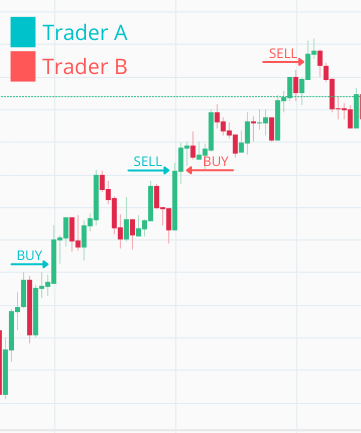
\includegraphics{images/chapter_06_01_current_buy_price.png}

The \texttt{Naive.Trader} process(marked in above diagram with blue color) at the arrival of the first trade event, immediately places a buy order at the current price. At the moment when buy order gets filled, it places sell order which later also gets filled.

The Trader A exits and a new trader B is started which again immediately places a buy order \emph{at the same price} as the previous trader just sold. When this gets filled sell order get's placed and loop continues on and on.

We can see that there's a problem here as we just paid a fee twice(once for selling by the Trader A and once for buying by the Trader B) without really gaining anything(the Trader A could just hold the currency and could simply cash in on double profit in this specific situation).

The solution is to be more clever about our buy order's price. The idea is simple, instead of placing a new buy order at the current price(price from the last TradeEvent), we will introduce a \texttt{buy\_down\_interval}:

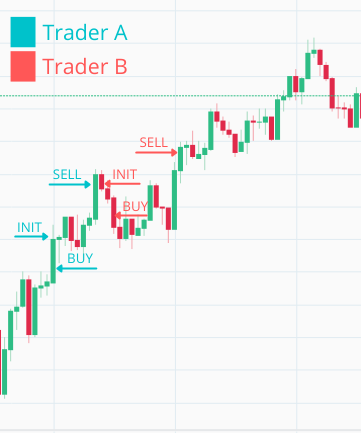
\includegraphics{images/chapter_06_02_rebuy_expl.png}

So every new \texttt{Naive.Trader} process as it receives first trade event, trader will take it's price and will calculate an decreased price by using the \texttt{buy\_down\_interval} value(for example 0.005 would be 0.5\%) and place a buy order at that calculated price.

When looking at the chart above we can figure out that \texttt{buy\_down\_interval} should never be smaller than double the fee(at the moment of writting transaction fee is 0.1\%) that you are paying per transaction.

\hypertarget{naive.trader-implementation}{%
\section{\texorpdfstring{\texttt{Naive.Trader} implementation}{Naive.Trader implementation}}\label{naive.trader-implementation}}

Let's open the \texttt{Naive.Trader} module's file(\texttt{/apps/naive/lib/naive/trader.ex}) and add \texttt{buy\_down\_interval} to it's state:

\begin{Shaded}
\begin{Highlighting}[]
  \CommentTok{\# /apps/naive/lib/naive/trader.ex}
  \OperatorTok{...}
  \KeywordTok{defmodule} \ConstantTok{State} \KeywordTok{do}
    \OtherTok{@enforce\_keys}\NormalTok{ [}
      \VariableTok{:symbol}\NormalTok{,}
      \VariableTok{:buy\_down\_interval}\NormalTok{, }\CommentTok{\# \textless{}= add this line}
      \VariableTok{:profit\_interval}\NormalTok{,}
      \VariableTok{:tick\_size}
\NormalTok{    ]}
    \KeywordTok{defstruct}\NormalTok{ [}
      \VariableTok{:symbol}\NormalTok{,}
      \VariableTok{:buy\_order}\NormalTok{,}
      \VariableTok{:sell\_order}\NormalTok{,}
      \VariableTok{:buy\_down\_interval}\NormalTok{, }\CommentTok{\# \textless{}= add this line}
      \VariableTok{:profit\_interval}\NormalTok{,}
      \VariableTok{:tick\_size}
\NormalTok{    ]}
  \KeywordTok{end}
  \OperatorTok{...}
\end{Highlighting}
\end{Shaded}

Next, we need to update the initial \texttt{handle\_info/2} callback which places the buy order. We need to retrieve the \texttt{buy\_down\_interval} and the \texttt{tick\_size} from the \texttt{state} of the trader to be able to calculate the buy price. We will put the logic to calculate that price in a separate function at the end of the file:

\begin{Shaded}
\begin{Highlighting}[]
  \CommentTok{\# /apps/naive/lib/naive/trader.ex}
  \OperatorTok{...}
  \KeywordTok{def}\NormalTok{ handle\_info(}
\NormalTok{        \%}\ConstantTok{TradeEvent}\NormalTok{\{}\VariableTok{price:}\NormalTok{ price\},}
\NormalTok{        \%}\ConstantTok{State}\NormalTok{\{}
          \VariableTok{symbol:}\NormalTok{ symbol,}
          \VariableTok{buy\_order:} \ConstantTok{nil}\NormalTok{,}
          \VariableTok{buy\_down\_interval:}\NormalTok{ buy\_down\_interval, }\CommentTok{\# \textless{}= add this line}
          \VariableTok{tick\_size:}\NormalTok{ tick\_size                  }\CommentTok{\# \textless{}= add this line          }
\NormalTok{        \} }\OperatorTok{=}\NormalTok{ state}
\NormalTok{      ) }\KeywordTok{do}
\NormalTok{    price }\OperatorTok{=}\NormalTok{ calculate\_buy\_price(price, buy\_down\_interval, tick\_size)}
    \CommentTok{\# \^{} add above call}
    \OperatorTok{...}
\end{Highlighting}
\end{Shaded}

To calculate the buy price we will use a very similar method to the one used
before to calculate the sell price. First, we will need to cast all variables
into the \texttt{Decimal} structs and then, we will simply subtract the \texttt{buy\_down\_interval} of the price from the price. The number that we will end up with won't necessarily be a legal price as every price needs to be divisible by the \texttt{tick\_size} which we will assure in the last calculation:

\begin{Shaded}
\begin{Highlighting}[]
  \CommentTok{\# /apps/naive/lib/naive/trader.ex}
  \OperatorTok{...}
  \KeywordTok{defp}\NormalTok{ calculate\_buy\_price(price, buy\_down\_interval, tick\_size) }\KeywordTok{do}
\NormalTok{    current\_price }\OperatorTok{=}\NormalTok{ D}\OperatorTok{.}\NormalTok{new(price)}

    \CommentTok{\# not necessarily legal price}
\NormalTok{    exact\_buy\_price }\OperatorTok{=}
\NormalTok{      D}\OperatorTok{.}\NormalTok{sub(}
\NormalTok{        current\_price,}
\NormalTok{        D}\OperatorTok{.}\NormalTok{mult(current\_price, buy\_down\_interval)}
\NormalTok{      )}

\NormalTok{    D}\OperatorTok{.}\NormalTok{to\_float(}
\NormalTok{      D}\OperatorTok{.}\NormalTok{mult(}
\NormalTok{        D}\OperatorTok{.}\NormalTok{div\_int(exact\_buy\_price, tick\_size),}
\NormalTok{        tick\_size}
\NormalTok{      )}
\NormalTok{    )}
  \KeywordTok{end}
  \OperatorTok{...}
\end{Highlighting}
\end{Shaded}

\hypertarget{naive.leader-implementation}{%
\section{\texorpdfstring{\texttt{Naive.Leader} implementation}{Naive.Leader implementation}}\label{naive.leader-implementation}}

Next we need to update the \texttt{Naive.Leader} as it needs to add \texttt{buy\_down\_interval} to the \texttt{Naive.Trader}'s state:

\begin{Shaded}
\begin{Highlighting}[]
  \CommentTok{\# /apps/naive/lib/naive/leader.ex}
  \KeywordTok{defp}\NormalTok{ fetch\_symbol\_settings(symbol) }\KeywordTok{do}
    \OperatorTok{...}

\NormalTok{    \%\{}
      \VariableTok{chunks:} \DecValTok{1}\NormalTok{,}
      \VariableTok{buy\_down\_interval:} \ConstantTok{Decimal}\OperatorTok{.}\NormalTok{new(}\StringTok{"0.0001"}\NormalTok{), }\CommentTok{\# \textless{}= add this line}
      \CommentTok{\# {-}0.12\% for quick testing}
      \VariableTok{profit\_interval:} \ConstantTok{Decimal}\OperatorTok{.}\NormalTok{new(}\StringTok{"{-}0.0012"}\NormalTok{),}
      \VariableTok{tick\_size:}\NormalTok{ tick\_size}
\NormalTok{    \}}
  \KeywordTok{end}  
  \OperatorTok{...}
\end{Highlighting}
\end{Shaded}

\hypertarget{iex-testing-1}{%
\subsection{IEx testing}\label{iex-testing-1}}

That finishes the \texttt{buy\_down\_interval} implementation, we will jump into iex session to see how it works, but before that for a moment we will change the logging level to \texttt{debug} to see current prices:

\begin{Shaded}
\begin{Highlighting}[]
\CommentTok{\# config/config.exs}
\OperatorTok{...}
\NormalTok{config }\VariableTok{:logger}\NormalTok{,}
  \VariableTok{level:} \VariableTok{:debug} \CommentTok{\# \textless{}= updated for our manual test}
\OperatorTok{...}
\end{Highlighting}
\end{Shaded}

After starting the streaming we should start seeing log messages with current prices. As we updated our implementation we should place our buy order below current price as it's visible below:

\begin{Shaded}
\begin{Highlighting}[]
\ExtensionTok{$}\NormalTok{ iex }\AttributeTok{{-}S}\NormalTok{ mix}
\ExtensionTok{...}
\ExtensionTok{iex}\ErrorTok{(}\ExtensionTok{1}\KeywordTok{)}\OperatorTok{\textgreater{}}\NormalTok{ Streamer.start\_streaming}\KeywordTok{(}\StringTok{"FLMUSDT"}\KeywordTok{)}
\ExtensionTok{\{:ok,} \CommentTok{\#PID\textless{}0.313.0\textgreater{}\}}
\ExtensionTok{iex}\ErrorTok{(}\ExtensionTok{2}\KeywordTok{)}\OperatorTok{\textgreater{}}\NormalTok{ Naive.start\_trading}\KeywordTok{(}\StringTok{"FLMUSDT"}\KeywordTok{)}
\ExtensionTok{21:16:14.829}\NormalTok{ [info]  Starting new supervision tree to trade on FLMUSDT}
\ExtensionTok{...}
\ExtensionTok{21:16:16.755}\NormalTok{ [info]  Initializing new trader for FLMUSDT}
\ExtensionTok{...}
\ExtensionTok{21:16:20.000}\NormalTok{ [debug] Trade event received FLMUSDT@0.15180000}
\ExtensionTok{21:16:20.009}\NormalTok{ [info]  Placing BUY order for FLMUSDT @ 0.1517, quantity: 100}
\end{Highlighting}
\end{Shaded}

As we can see our \texttt{Naive.Trader} process placed an buy order below the current price (based on most recent trade event received)

{[}Note{]} Please remember to revert the change to logger level as otherwise there's too much noise in the logs.

{[}Note 2{]} Please remember to run \texttt{mix\ format} to keep things nice and tidy.

Source code for this chapter can be found at \href{https://github.com/frathon/create-a-cryptocurrency-trading-bot-in-elixir-source-code/tree/chapter_06}{Github}

\hypertarget{introduce-a-trader-budget-and-calculating-the-quantity}{%
\chapter{Introduce a trader budget and calculating the quantity}\label{introduce-a-trader-budget-and-calculating-the-quantity}}

\hypertarget{objectives-6}{%
\section{Objectives}\label{objectives-6}}

\begin{itemize}
\tightlist
\item
  fetch step\_size
\item
  append budget and step\_size to the \texttt{Trader}'s state compiled by the \texttt{Leader}
\item
  append budget and step\_size to the \texttt{Trader}'s state
\item
  calculate quantity
\end{itemize}

\hypertarget{fetch-step_size}{%
\section{\texorpdfstring{Fetch \texttt{step\_size}}{Fetch step\_size}}\label{fetch-step_size}}

In 2nd chapter we hardcoded \texttt{quantity} to 100, it's time to refactor that. We will need \texttt{step\_size} information from the Binance which we are
already retrieving together with \texttt{tick\_size} in the \texttt{exchangeInfo} call(but not getting it out from the response). So we will rename the \texttt{fetch\_tick\_size/1} function to \texttt{fetch\_symbol\_filters/1} which will allow us to return multiple filters(\texttt{tick\_size} and \texttt{step\_size}) from that function.

\begin{Shaded}
\begin{Highlighting}[]
  \CommentTok{\# /apps/naive/lib/naive/leader.ex}
  \OperatorTok{...}
  \KeywordTok{defp}\NormalTok{ fetch\_symbol\_settings(symbol) }\KeywordTok{do}
\NormalTok{    symbol\_filters }\OperatorTok{=}\NormalTok{ fetch\_symbol\_filters(symbol) }\CommentTok{\# \textless{}= updated fetch\_tick\_size}
    
    \ConstantTok{Map}\OperatorTok{.}\NormalTok{merge(}
\NormalTok{      \%\{}
        \VariableTok{chunks:} \DecValTok{1}\NormalTok{,}
        \VariableTok{budget:} \DecValTok{20}\NormalTok{,}
        \VariableTok{buy\_down\_interval:} \ConstantTok{Decimal}\OperatorTok{.}\NormalTok{new(}\StringTok{"0.0001"}\NormalTok{),}
        \CommentTok{\# {-}0.12\% for quick testing}
        \VariableTok{profit\_interval:} \ConstantTok{Decimal}\OperatorTok{.}\NormalTok{new(}\StringTok{"{-}0.0012"}\NormalTok{)}
\NormalTok{      \},}
\NormalTok{      symbol\_filters}
\NormalTok{    )}
  \KeywordTok{end}

  \KeywordTok{defp}\NormalTok{ fetch\_symbol\_filters(symbol) }\KeywordTok{do}  \CommentTok{\# \textless{}= updated fetch\_tick\_size}
\NormalTok{    symbol\_filters }\OperatorTok{=}
      \OtherTok{@binance\_client}\OperatorTok{.}\NormalTok{get\_exchange\_info()}
      \OperatorTok{|\textgreater{}}\NormalTok{ elem(}\DecValTok{1}\NormalTok{)}
      \OperatorTok{|\textgreater{}} \ConstantTok{Map}\OperatorTok{.}\NormalTok{get(}\VariableTok{:symbols}\NormalTok{)}
      \OperatorTok{|\textgreater{}} \ConstantTok{Enum}\OperatorTok{.}\NormalTok{find(}\OperatorTok{\&}\NormalTok{(}\OperatorTok{\&}\DecValTok{1}\NormalTok{[}\StringTok{"symbol"}\NormalTok{] }\OperatorTok{==}\NormalTok{ symbol))}
      \OperatorTok{|\textgreater{}} \ConstantTok{Map}\OperatorTok{.}\NormalTok{get(}\StringTok{"filters"}\NormalTok{)}

\NormalTok{    tick\_size }\OperatorTok{=}
\NormalTok{      symbol\_filters}
      \OperatorTok{|\textgreater{}} \ConstantTok{Enum}\OperatorTok{.}\NormalTok{find(}\OperatorTok{\&}\NormalTok{(}\OperatorTok{\&}\DecValTok{1}\NormalTok{[}\StringTok{"filterType"}\NormalTok{] }\OperatorTok{==} \StringTok{"PRICE\_FILTER"}\NormalTok{))}
      \OperatorTok{|\textgreater{}} \ConstantTok{Map}\OperatorTok{.}\NormalTok{get(}\StringTok{"tickSize"}\NormalTok{)}
      \OperatorTok{|\textgreater{}} \ConstantTok{Decimal}\OperatorTok{.}\NormalTok{new()}

\NormalTok{    step\_size }\OperatorTok{=}
\NormalTok{      symbol\_filters}
      \OperatorTok{|\textgreater{}} \ConstantTok{Enum}\OperatorTok{.}\NormalTok{find(}\OperatorTok{\&}\NormalTok{(}\OperatorTok{\&}\DecValTok{1}\NormalTok{[}\StringTok{"filterType"}\NormalTok{] }\OperatorTok{==} \StringTok{"LOT\_SIZE"}\NormalTok{))}
      \OperatorTok{|\textgreater{}} \ConstantTok{Map}\OperatorTok{.}\NormalTok{get(}\StringTok{"stepSize"}\NormalTok{)}
      \OperatorTok{|\textgreater{}} \ConstantTok{Decimal}\OperatorTok{.}\NormalTok{new()}

\NormalTok{    \%\{}
      \VariableTok{tick\_size:}\NormalTok{ tick\_size,}
      \VariableTok{step\_size:}\NormalTok{ step\_size}
\NormalTok{    \}}
  \KeywordTok{end}
\end{Highlighting}
\end{Shaded}

Instead of reassigning the filters one by one into the settings, we will merge them together(\#1). Additionally, we will introduce a \texttt{budget}(\#2) which will be shared across all traders of the symbol. Also, we don't need to assign \texttt{tick\_size} here as it's part of the settings that are merged.

\hypertarget{append-budget-and-step_size-to-the-traders-state-inside-the-leader}{%
\section{\texorpdfstring{Append \texttt{budget} and \texttt{step\_size} to the \texttt{Trader}'s state inside the \texttt{Leader}}{Append budget and step\_size to the Trader's state inside the Leader}}\label{append-budget-and-step_size-to-the-traders-state-inside-the-leader}}

The \texttt{budget} needs to be added to the \texttt{\%State\{\}}(\texttt{step\_size} will be automatically passed on by \texttt{struct/2}) of the trader inside \texttt{fresh\_trader\_state/1}(where we initialize the state of traders). Before we will assign it we need to divide it by number of chunks as each trader gets only a chunk of the budget:

\begin{Shaded}
\begin{Highlighting}[]
  \CommentTok{\# /apps/naive/lib/naive/leader.ex}
  \KeywordTok{defp}\NormalTok{ fresh\_trader\_state(settings) }\KeywordTok{do}
\NormalTok{    \%\{}
\NormalTok{      struct(}\ConstantTok{Trader}\OperatorTok{.}\ConstantTok{State}\NormalTok{, settings) }\OperatorTok{|}
      \VariableTok{budget:}\NormalTok{ D}\OperatorTok{.}\NormalTok{div(settings}\OperatorTok{.}\NormalTok{budget, settings}\OperatorTok{.}\NormalTok{chunks)}
\NormalTok{    \}}
  \KeywordTok{end}
\end{Highlighting}
\end{Shaded}

In the code above we are using the \texttt{Decimal} module(aliased as \texttt{D}) to calculate the budget - we need to alias it at the top of \texttt{Naive.Leader}'s file:

\begin{Shaded}
\begin{Highlighting}[]
\CommentTok{\# /apps/naive/lib/naive/leader.ex}
\KeywordTok{defmodule} \ConstantTok{Naive}\OperatorTok{.}\ConstantTok{Leader} \KeywordTok{do}
  \ImportTok{use} \ConstantTok{GenServer}

  \ImportTok{alias} \ConstantTok{Decimal}\NormalTok{, }\VariableTok{as:}\NormalTok{ D }\CommentTok{\# \textless{}= add this line}
  \ImportTok{alias} \ConstantTok{Naive}\OperatorTok{.}\ConstantTok{Trader}
  \OperatorTok{...}
\end{Highlighting}
\end{Shaded}

\hypertarget{append-budget-and-step_size-to-the-traders-state}{%
\section{\texorpdfstring{Append \texttt{budget} and \texttt{step\_size} to the \texttt{Trader}'s state}{Append budget and step\_size to the Trader's state}}\label{append-budget-and-step_size-to-the-traders-state}}

We need to add both \texttt{budget} and \texttt{step\_size} to the \texttt{Naive.Trader}'s state struct:

\begin{Shaded}
\begin{Highlighting}[]
  \CommentTok{\# /apps/naive/lib/naive/trader.ex}
  \OperatorTok{...}
  \KeywordTok{defmodule} \ConstantTok{State} \KeywordTok{do}
    \OtherTok{@enforce\_keys}\NormalTok{ [}
      \VariableTok{:symbol}\NormalTok{,}
      \VariableTok{:budget}\NormalTok{, }\CommentTok{\# \textless{}= add this line}
      \VariableTok{:buy\_down\_interval}\NormalTok{,}
      \VariableTok{:profit\_interval}\NormalTok{,}
      \VariableTok{:tick\_size}\NormalTok{,}
      \VariableTok{:step\_size} \CommentTok{\# \textless{}= add this line and comma above}
\NormalTok{    ]}
    \KeywordTok{defstruct}\NormalTok{ [}
      \VariableTok{:symbol}\NormalTok{,}
      \VariableTok{:budget}\NormalTok{, }\CommentTok{\# \textless{}= add this line}
      \VariableTok{:buy\_order}\NormalTok{,}
      \VariableTok{:sell\_order}\NormalTok{,}
      \VariableTok{:buy\_down\_interval}\NormalTok{,}
      \VariableTok{:profit\_interval}\NormalTok{,}
      \VariableTok{:tick\_size}\NormalTok{,}
      \VariableTok{:step\_size} \CommentTok{\# \textless{}= add this line and comma above}
\NormalTok{    ]}
  \KeywordTok{end}
  \OperatorTok{...}
\end{Highlighting}
\end{Shaded}

\hypertarget{calculate-quantity}{%
\section{Calculate quantity}\label{calculate-quantity}}

Jumping back to the \texttt{handle\_info/2} where the \texttt{Naive.Trader} places a buy order, we need to pattern match on the \texttt{step\_size} and \texttt{budget} then we will be able to swap hardcoded quantity with result of calling the \texttt{calculate\_quantity/3} function:

\begin{Shaded}
\begin{Highlighting}[]
  \CommentTok{\# /apps/naive/lib/naive/trader.ex}
  \OperatorTok{...}
  \KeywordTok{def}\NormalTok{ handle\_info(}
\NormalTok{        \%}\ConstantTok{TradeEvent}\NormalTok{\{}\VariableTok{price:}\NormalTok{ price\},}
\NormalTok{        \%}\ConstantTok{State}\NormalTok{\{}
          \VariableTok{symbol:}\NormalTok{ symbol,}
          \VariableTok{budget:}\NormalTok{ budget, }\CommentTok{\# \textless{}= add this line}
          \VariableTok{buy\_order:} \ConstantTok{nil}\NormalTok{,}
          \VariableTok{buy\_down\_interval:}\NormalTok{ buy\_down\_interval,}
          \VariableTok{tick\_size:}\NormalTok{ tick\_size,}
          \VariableTok{step\_size:}\NormalTok{ step\_size }\CommentTok{\# \textless{}= add this line}
\NormalTok{        \} }\OperatorTok{=}\NormalTok{ state}
\NormalTok{      ) }\KeywordTok{do}
    \OperatorTok{...}
\NormalTok{    quantity }\OperatorTok{=}\NormalTok{ calculate\_quantity(budget, price, step\_size)}
    \OperatorTok{...}
\end{Highlighting}
\end{Shaded}

To calculate quantity we will just divide the \texttt{budget} by the \texttt{price} with a caveat that it's possible (as with calculating the price) that it's not a legal quantity value as it needs to be divisiable by \texttt{step\_size}:

\begin{Shaded}
\begin{Highlighting}[]
  \CommentTok{\# /apps/naive/lib/naive/trader.ex}
  \CommentTok{\# add below at the bottom of the file}
  \OperatorTok{...}
  \KeywordTok{defp}\NormalTok{ calculate\_quantity(budget, price, step\_size) }\KeywordTok{do}
\NormalTok{    price }\OperatorTok{=}\NormalTok{ D}\OperatorTok{.}\NormalTok{from\_float(price)}

    \CommentTok{\# not necessarily legal quantity}
\NormalTok{    exact\_target\_quantity }\OperatorTok{=}\NormalTok{ D}\OperatorTok{.}\NormalTok{div(budget, price)}

\NormalTok{    D}\OperatorTok{.}\NormalTok{to\_float(}
\NormalTok{      D}\OperatorTok{.}\NormalTok{mult(}
\NormalTok{        D}\OperatorTok{.}\NormalTok{div\_int(exact\_target\_quantity, step),}
\NormalTok{        step}
\NormalTok{      )}
\NormalTok{    )}
  \KeywordTok{end}
\end{Highlighting}
\end{Shaded}

\hypertarget{iex-testing-2}{%
\subsection{IEx testing}\label{iex-testing-2}}

That finishes the \texttt{quantity}(and \texttt{budget}) implementation, we will jump into iex session to see how it works.

First, start the streaming and trading on the same symbol and moment later you should see variable amount of quantity that more or less uses full allowed budget:

\begin{Shaded}
\begin{Highlighting}[]
\ExtensionTok{$}\NormalTok{ iex }\AttributeTok{{-}S}\NormalTok{ mix}
\ExtensionTok{...}
\ExtensionTok{iex}\ErrorTok{(}\ExtensionTok{1}\KeywordTok{)}\OperatorTok{\textgreater{}}\NormalTok{ Streamer.start\_streaming}\KeywordTok{(}\StringTok{"XRPUSDT"}\KeywordTok{)}
\ExtensionTok{\{:ok,} \CommentTok{\#PID\textless{}0.313.0\textgreater{}\}}
\ExtensionTok{iex}\ErrorTok{(}\ExtensionTok{2}\KeywordTok{)}\OperatorTok{\textgreater{}}\NormalTok{ Naive.start\_trading}\KeywordTok{(}\StringTok{"XRPUSDT"}\KeywordTok{)}
\ExtensionTok{21:16:14.829}\NormalTok{ [info]  Starting new supervision tree to trade on XRPUSDT}
\ExtensionTok{21:16:16.755}\NormalTok{ [info]  Initializing new trader for XRPUSDT}
\ExtensionTok{21:16:20.009}\NormalTok{ [info]  Placing BUY order for XRPUSDT @ 0.29506, quantity: 67.7}
\ExtensionTok{21:16:23.456}\NormalTok{ [info]  Buy order filled, placing SELL order for XRPUSDT @ 0.29529, quantity: 67.7}
\end{Highlighting}
\end{Shaded}

As we can see our \texttt{Naive.Trader} process is now buying and selling based on passed budget.

{[}Note{]} Please remember to run \texttt{mix\ format} to keep things nice and tidy.

Source code for this chapter can be found at \href{https://github.com/frathon/create-a-cryptocurrency-trading-bot-in-elixir-source-code/tree/chapter_07}{Github}

\hypertarget{add-support-for-multiple-transactions-per-order}{%
\chapter{Add support for multiple transactions per order}\label{add-support-for-multiple-transactions-per-order}}

\hypertarget{objectives-7}{%
\section{Objectives}\label{objectives-7}}

\begin{itemize}
\tightlist
\item
  describe issue with current implementation
\item
  improve buy order filled callback
\item
  implement buy order ``filled'' callback
\item
  improve sell order callback
\end{itemize}

\hypertarget{issue-with-the-current-implementation}{%
\section{Issue with the current implementation}\label{issue-with-the-current-implementation}}

Currently, \texttt{Naive.Trader} process is placing a buy order and it's assuming that it will be filled by a \emph{single} opposite sell order(we are pattern matching on quantity to confirm that):

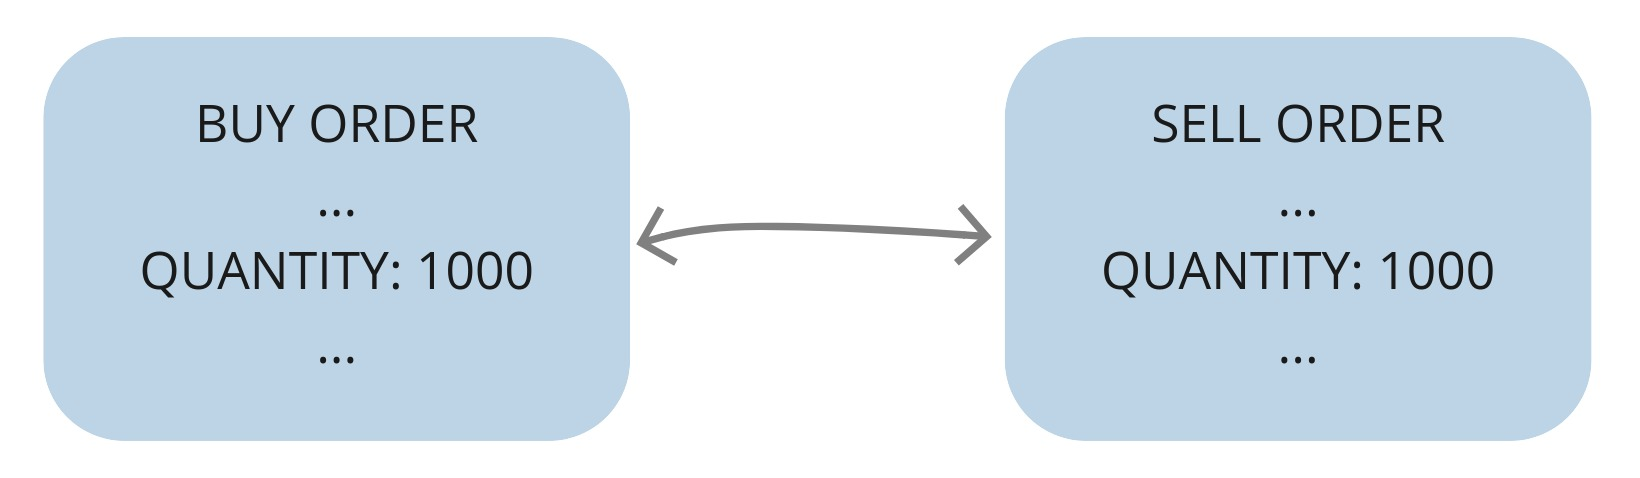
\includegraphics{images/chapter_08_01_single_transaction.png}

Here we can see our buy order for 1000 units(on the left) and other trader's sell order(on the right) for 1000 units. This(order fully filled in single transaction) is a case most of the time but it's not ALWAYS the case.

Sometimes our order will be filled by two or more transactions:

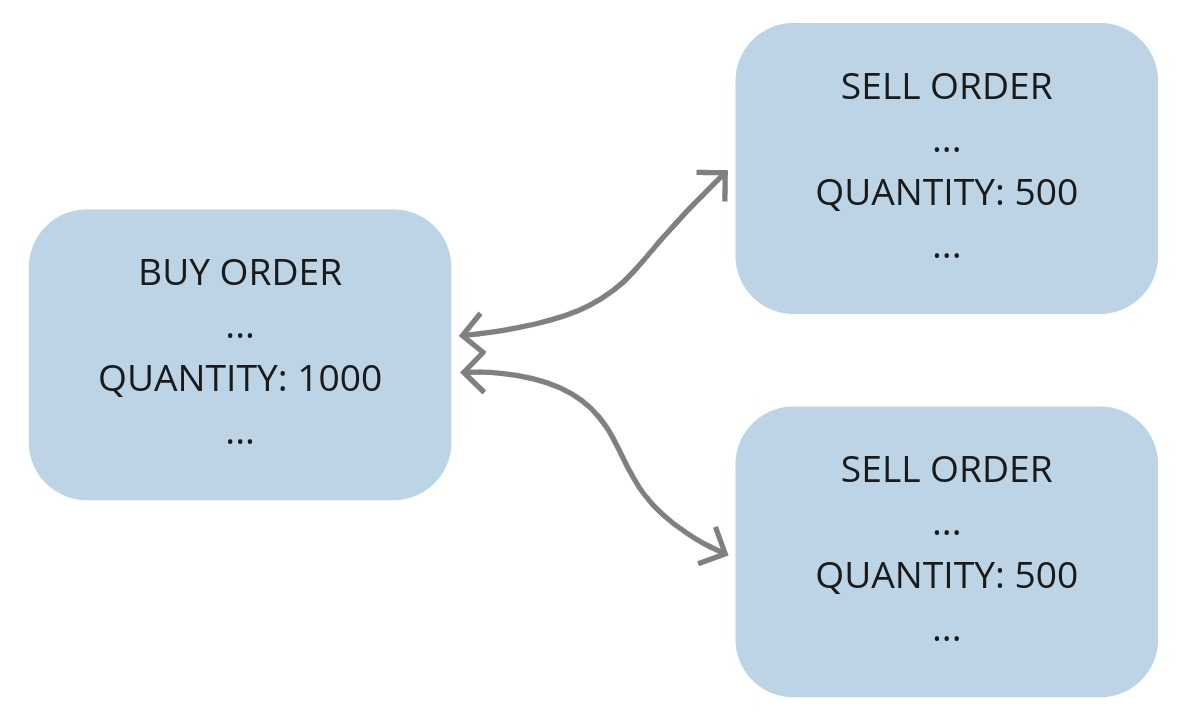
\includegraphics{images/chapter_08_02_multiple_transactions_per_order.png}

The easiest and the safest way to check has this event filled our order fully is to fetch our order again from Binance at the moment when trade event filling our order arrives.

Problem with this approach is that sometimes we will run into a race condition:

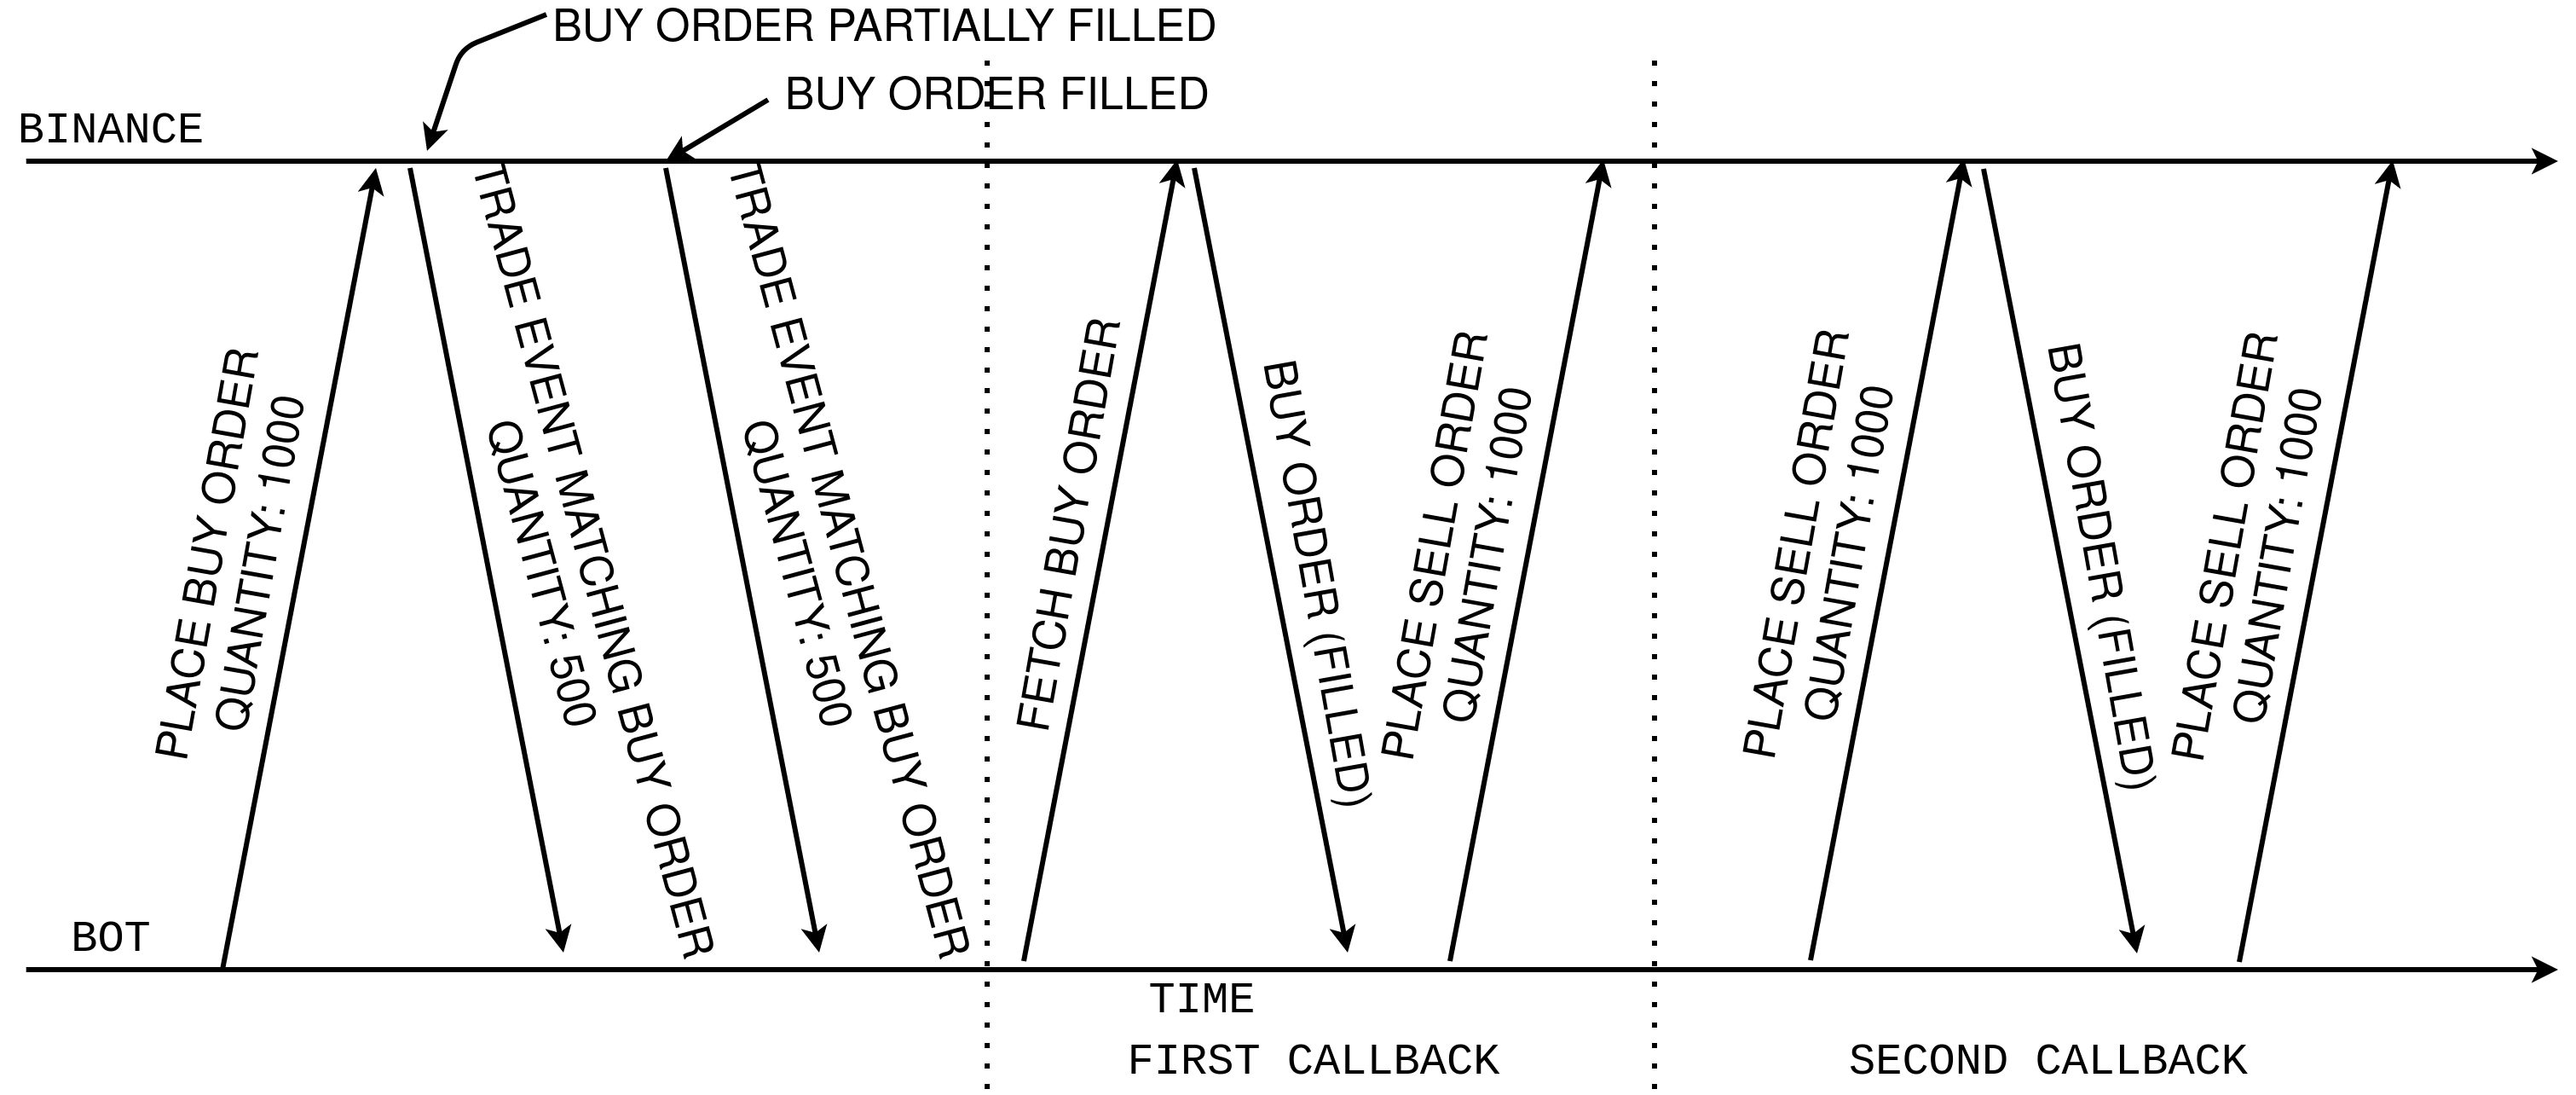
\includegraphics{images/chapter_08_03_race_condition_timeline.png}

From the left, first, we are sending a buy order for quantity 1000 to the Binance. It hangs for a while until it gets filled by 2 transactions that happened very quickly. Quickly enough for us to receive both messages almost in the same moment.

When our bot will handle the first one it will fetch our the buy order which is already filled. It will cause the trader to place a sell order but then the there's another trade event waiting in the message box. It will be handled by another callback that will again fetch order and place another sell order to be placed and that's obviously not correct.

What we need to do is to update the status of the buy order after the first fetch(if it's filled) so when second trade event arrives we will ignore it(this will require additional callback).

The same issue will appear when placing sell order and dealing multiple simultaneous transaction.

\hypertarget{improve-buy-order-filled-callback}{%
\section{Improve buy order filled callback}\label{improve-buy-order-filled-callback}}

First, we need to modify the callback which monitors incoming trade events for ones filling it's buy order and then places sell order. We need to remove pattern matching assuming that a single trade event will fill our buy order - we need to drop quantity check as well as add

\begin{Shaded}
\begin{Highlighting}[]
  \CommentTok{\# /apps/naive/lib/naive/trader.ex}
  \KeywordTok{def}\NormalTok{ handle\_info(}
\NormalTok{        \%}\ConstantTok{TradeEvent}\NormalTok{\{}
          \VariableTok{buyer\_order\_id:}\NormalTok{ order\_id }\CommentTok{\# \textless{}= quantity got removed from here}
\NormalTok{        \},}
\NormalTok{        \%}\ConstantTok{State}\NormalTok{\{}
          \VariableTok{symbol:}\NormalTok{ symbol,}
          \VariableTok{buy\_order:}
\NormalTok{            \%}\ConstantTok{Binance}\OperatorTok{.}\ConstantTok{OrderResponse}\NormalTok{\{}
              \VariableTok{price:}\NormalTok{ buy\_price,}
              \VariableTok{order\_id:}\NormalTok{ order\_id,}
              \VariableTok{orig\_qty:}\NormalTok{ quantity,}
              \VariableTok{transact\_time:}\NormalTok{ timestamp }\CommentTok{\# \textless{}= timestamp added to query order}
\NormalTok{            \} }\OperatorTok{=}\NormalTok{ buy\_order, }\CommentTok{\# \textless{}= buy order to update it}
          \VariableTok{profit\_interval:}\NormalTok{ profit\_interval,}
          \VariableTok{tick\_size:}\NormalTok{ tick\_size}
\NormalTok{        \} }\OperatorTok{=}\NormalTok{ state}
\NormalTok{      ) }\KeywordTok{do}
\end{Highlighting}
\end{Shaded}

Now we can fetch our buy order to check is it already filled. We will get the \texttt{Binance.Order} struct instead of the \texttt{Binance.OrderResponse} that we normally deal with. At this moment we will simply update our \texttt{Binance.OrderResponse} struct from state:

\begin{Shaded}
\begin{Highlighting}[]
  \CommentTok{\# /apps/naive/lib/naive/trader.ex}
  \CommentTok{\# inside the same callback}
  \KeywordTok{def}\NormalTok{ handle\_info(}
      \OperatorTok{...}
\NormalTok{      ) }\KeywordTok{do}
\NormalTok{    \{}\VariableTok{:ok}\NormalTok{, \%}\ConstantTok{Binance}\OperatorTok{.}\ConstantTok{Order}\NormalTok{\{\} }\OperatorTok{=}\NormalTok{ current\_buy\_order\} }\OperatorTok{=}
      \OtherTok{@binance\_client}\OperatorTok{.}\NormalTok{get\_order(}
\NormalTok{        symbol,}
\NormalTok{        timestamp,}
\NormalTok{        order\_id}
\NormalTok{      )}
    
\NormalTok{    buy\_order }\OperatorTok{=}\NormalTok{ \%\{buy\_order }\OperatorTok{|} \VariableTok{status:}\NormalTok{ current\_buy\_order}\OperatorTok{.}\NormalTok{status\}}
    \OperatorTok{...}
\end{Highlighting}
\end{Shaded}

The rest of the logic inside this callback will depend on the \texttt{status} of the buy order. If our buy order is ``filled'' we would like to follow the existing logic but also update \texttt{buy\_order} field inside the state of the trader process. On the other hand if our order is not yet filled the only thing to do is to update \texttt{buy\_order} field inside the state of the Trader process. Here's and updated body below above changes(few variables got renamed for clarity as we are now fetch the order):

\begin{Shaded}
\begin{Highlighting}[]
  \CommentTok{\# /apps/naive/lib/naive/trader.ex}
  \CommentTok{\# inside the same callback}
\NormalTok{  buy\_order }\OperatorTok{=} \OperatorTok{....}

\NormalTok{    \{}\VariableTok{:ok}\NormalTok{, new\_state\} }\OperatorTok{=}
      \ControlFlowTok{if}\NormalTok{ buy\_order}\OperatorTok{.}\NormalTok{status }\OperatorTok{==} \StringTok{"FILLED"} \KeywordTok{do}
\NormalTok{        sell\_price }\OperatorTok{=}\NormalTok{ calculate\_sell\_price(buy\_price, profit\_interval, tick\_size)}

        \ConstantTok{Logger}\OperatorTok{.}\NormalTok{info(}
          \StringTok{"Buy order filled, placing SELL order for "} \OperatorTok{\textless{}\textgreater{}}
            \StringTok{"}\OtherTok{\#\{}\NormalTok{symbol}\OtherTok{\}}\StringTok{ @ }\OtherTok{\#\{}\NormalTok{sell\_price}\OtherTok{\}}\StringTok{, quantity: }\OtherTok{\#\{}\NormalTok{quantity}\OtherTok{\}}\StringTok{"}
\NormalTok{        )}

\NormalTok{        \{}\VariableTok{:ok}\NormalTok{, \%}\ConstantTok{Binance}\OperatorTok{.}\ConstantTok{OrderResponse}\NormalTok{\{\} }\OperatorTok{=}\NormalTok{ order\} }\OperatorTok{=}
          \OtherTok{@binance\_client}\OperatorTok{.}\NormalTok{order\_limit\_sell(symbol, quantity, sell\_price, }\StringTok{"GTC"}\NormalTok{)}

\NormalTok{        \{}\VariableTok{:ok}\NormalTok{, \%\{state }\OperatorTok{|} \VariableTok{buy\_order:}\NormalTok{ buy\_order, }\VariableTok{sell\_order:}\NormalTok{ order\}\}}
      \ControlFlowTok{else}
        \ConstantTok{Logger}\OperatorTok{.}\NormalTok{info(}\StringTok{"Buy order partially filled"}\NormalTok{)}
\NormalTok{        \{}\VariableTok{:ok}\NormalTok{, \%\{state }\OperatorTok{|} \VariableTok{buy\_order:}\NormalTok{ buy\_order\}\}}
      \KeywordTok{end}

    \ConstantTok{Naive}\OperatorTok{.}\ConstantTok{Leader}\OperatorTok{.}\NormalTok{notify(}\VariableTok{:trader\_state\_updated}\NormalTok{, new\_state)}
\NormalTok{    \{}\VariableTok{:noreply}\NormalTok{, new\_state\}}
  \KeywordTok{end}
\end{Highlighting}
\end{Shaded}

As we are branching our logic and both paths are updating the state, we will return it together with an \texttt{:ok} atom to be able to pattern match it and assign as a new state.

\hypertarget{implement-buy-order-filled-callback}{%
\section{Implement buy order ``filled'' callback}\label{implement-buy-order-filled-callback}}

Above callback covers the case where we will get multiple transactions filling our buy order. We aren't yet convering for the race condition described at the begining of this chapter. When another trade event matching \texttt{buyer\_order\_id} would arrive, above callback would be used and another sell order would be placed. To avoid that we need to add a new callback \emph{ABOVE} the one that we just edited that will match \texttt{buyer\_order\_id} together with ``filled'' \texttt{status} and it will simply ignore that trade event as we know that sell event needed to be placed by previous trade event:

\begin{Shaded}
\begin{Highlighting}[]
  \CommentTok{\# /apps/naive/lib/naive/trader.ex}
  \CommentTok{\# place this callback ABOVE callback from previous section}
  \KeywordTok{def}\NormalTok{ handle\_info(}
\NormalTok{        \%}\ConstantTok{Streamer}\OperatorTok{.}\ConstantTok{Binance}\OperatorTok{.}\ConstantTok{TradeEvent}\NormalTok{\{}
          \VariableTok{buyer\_order\_id:}\NormalTok{ order\_id}
\NormalTok{        \},}
\NormalTok{        \%}\ConstantTok{State}\NormalTok{\{}
          \VariableTok{buy\_order:}\NormalTok{ \%}\ConstantTok{Binance}\OperatorTok{.}\ConstantTok{OrderResponse}\NormalTok{\{}
            \VariableTok{order\_id:}\NormalTok{ order\_id, }\CommentTok{\# \textless{}= confirms that it\textquotesingle{}s event for buy order}
            \VariableTok{status:} \StringTok{"FILLED"} \CommentTok{\# \textless{}= confirms buy order filled}
\NormalTok{          \},}
          \VariableTok{sell\_order:}\NormalTok{ \%}\ConstantTok{Binance}\OperatorTok{.}\ConstantTok{OrderResponse}\NormalTok{\{\} }\CommentTok{\# \textless{}= confirms sell order placed}
\NormalTok{        \} }\OperatorTok{=}\NormalTok{ state}
\NormalTok{      ) }\KeywordTok{do}
\NormalTok{    \{}\VariableTok{:noreply}\NormalTok{, state\}}
  \KeywordTok{end}
\end{Highlighting}
\end{Shaded}

\hypertarget{improve-sell-order-callback}{%
\section{Improve sell order callback}\label{improve-sell-order-callback}}

Let's move on to the callback where the trader receives trade event matching sell order's id (about line 135 inside the \texttt{Naive.Trader} module).

We need to modify the header of our callback in the following ways:
- drop the both pattern matches on \texttt{quantity} as we already know that trade event could partially fill our order (\#1)
- get \texttt{symbol} out of state (\#2)
- get \texttt{transact\_time} out of the \texttt{sell\_order} (used to fetch \texttt{get\_order}) (\#3)
- assign \texttt{sell\_order} to a variable (\#4)

\begin{Shaded}
\begin{Highlighting}[]
  \CommentTok{\# /apps/naive/lib/naive/trader.ex}
  \KeywordTok{def}\NormalTok{ handle\_info(}
\NormalTok{        \%}\ConstantTok{TradeEvent}\NormalTok{\{}
          \VariableTok{seller\_order\_id:}\NormalTok{ order\_id }\CommentTok{\# \textasciigrave{}quantity\textasciigrave{} check removed below (\#1)}
\NormalTok{        \},}
\NormalTok{        \%}\ConstantTok{State}\NormalTok{\{}
          \VariableTok{symbol:}\NormalTok{ symbol, (}\CommentTok{\#2)}
          \VariableTok{sell\_order:}
\NormalTok{            \%}\ConstantTok{Binance}\OperatorTok{.}\ConstantTok{OrderResponse}\NormalTok{\{}
              \VariableTok{order\_id:}\NormalTok{ order\_id,}
              \VariableTok{transact\_time:}\NormalTok{ timestamp }\CommentTok{\# \textasciigrave{}transact\_time\textasciigrave{} to \textasciigrave{}get\_order\textasciigrave{} (\#3)}
\NormalTok{            \} }\OperatorTok{=}\NormalTok{ sell\_order }\CommentTok{\# to update order (\#4)}
\NormalTok{        \} }\OperatorTok{=}\NormalTok{ state}
\NormalTok{      ) }\KeywordTok{do}
\end{Highlighting}
\end{Shaded}

Moving lower to the body of the function, we need to:
- fetch current state of our sell order
- update \texttt{status} of our \texttt{sell\_order} from Trader's state
- branch out the logic based on \texttt{status} of the \texttt{sell\_order}:
* log and return the \texttt{:stop} atom to stop the GenServer
or
* update the state with new \texttt{sell\_order} and continue

Here's the full body of our callback:

\begin{Shaded}
\begin{Highlighting}[]
    \CommentTok{\# /apps/naive/lib/naive/trader.ex}
    \CommentTok{\# inside the callabck}
\NormalTok{    \{}\VariableTok{:ok}\NormalTok{, \%}\ConstantTok{Binance}\OperatorTok{.}\ConstantTok{Order}\NormalTok{\{\} }\OperatorTok{=}\NormalTok{ current\_sell\_order\} }\OperatorTok{=}
      \OtherTok{@binance\_client}\OperatorTok{.}\NormalTok{get\_order(}
\NormalTok{        symbol,}
\NormalTok{        timestamp,}
\NormalTok{        order\_id}
\NormalTok{      )}

\NormalTok{    sell\_order }\OperatorTok{=}\NormalTok{ \%\{sell\_order }\OperatorTok{|} \VariableTok{status:}\NormalTok{ current\_sell\_order}\OperatorTok{.}\NormalTok{status\}}

    \ControlFlowTok{if}\NormalTok{ sell\_order}\OperatorTok{.}\NormalTok{status }\OperatorTok{==} \StringTok{"FILLED"} \KeywordTok{do}
      \ConstantTok{Logger}\OperatorTok{.}\NormalTok{info(}\StringTok{"Trade finished, trader will now exit"}\NormalTok{)}
\NormalTok{      \{}\VariableTok{:stop}\NormalTok{, }\VariableTok{:normal}\NormalTok{, state\}}
    \ControlFlowTok{else}
      \ConstantTok{Logger}\OperatorTok{.}\NormalTok{info(}\StringTok{"Sell order partially filled"}\NormalTok{)}
\NormalTok{      new\_state }\OperatorTok{=}\NormalTok{ \%\{state }\OperatorTok{|} \VariableTok{sell\_order:}\NormalTok{ sell\_order\}}
\NormalTok{      \{}\VariableTok{:noreply}\NormalTok{, new\_state\}}
    \KeywordTok{end}
\end{Highlighting}
\end{Shaded}

\hypertarget{test-the-implementation-1}{%
\section{Test the implementation}\label{test-the-implementation-1}}

Testing this feature is a bit tricky as it requires trading on real Binance exachnge(as our BinanceMock always fills order with a single transaction) as well as race condition to happen :) Not that easy but even without race condition we should still test that code works as expected wiht BinanceMock:

\begin{Shaded}
\begin{Highlighting}[]
\ExtensionTok{$}\NormalTok{ iex }\AttributeTok{{-}S}\NormalTok{ mix}
\ExtensionTok{...}
\ExtensionTok{iex}\ErrorTok{(}\ExtensionTok{1}\KeywordTok{)}\OperatorTok{\textgreater{}}\NormalTok{ Naive.start\_trading}\KeywordTok{(}\StringTok{"XRPUSDT"}\KeywordTok{)}
\ExtensionTok{23:27:35.977}\NormalTok{ [info]  Starting new supervision tree to trade on XRPUSDT}
\ExtensionTok{\{:ok,} \CommentTok{\#PID\textless{}0.331.0\textgreater{}\}}
\ExtensionTok{23:27:39.073}\NormalTok{ [info]  Initializing new trader for XRPUSDT}
\ExtensionTok{iex}\ErrorTok{(}\ExtensionTok{2}\KeywordTok{)}\OperatorTok{\textgreater{}}\NormalTok{ Streamer.start\_streaming}\KeywordTok{(}\StringTok{"XRPUSDT"}\KeywordTok{)}
\ExtensionTok{\{:ok,} \CommentTok{\#PID\textless{}0.345.0\textgreater{}\}}
\ExtensionTok{23:31:57.044}\NormalTok{ [info]  Initializing new trader for XRPUSDT}
\ExtensionTok{23:31:57.888}\NormalTok{ [info]  Placing BUY order for XRPUSDT @ 0.28031, quantity: 71.3}
\ExtensionTok{23:32:01.023}\NormalTok{ [info]  Buy order filled, placing SELL order for XRPUSDT @ 0.28053, quantity: 71.30000000}
\ExtensionTok{23:33:08.865}\NormalTok{ [info]  Trade finished, trader will now exit}
\ExtensionTok{23:33:08.865}\NormalTok{ [info]  XRPUSDT Trader finished }\AttributeTok{{-}}\NormalTok{ restarting}
\end{Highlighting}
\end{Shaded}

{[}Note{]} Please remember to run \texttt{mix\ format} to keep things nice and tidy.

Source code for this chapter can be found at \href{https://github.com/frathon/create-a-cryptocurrency-trading-bot-in-elixir-source-code/tree/chapter_08}{Github}

\hypertarget{run-multiple-traders-in-parallel}{%
\chapter{Run multiple traders in parallel}\label{run-multiple-traders-in-parallel}}

\hypertarget{objectives-8}{%
\section{Objectives}\label{objectives-8}}

\begin{itemize}
\tightlist
\item
  describe and design the required functionality
\item
  implement rebuy in the \texttt{Naive.Trader}
\item
  implement rebuy in the \texttt{Naive.Leader}
\item
  improve logs by assigning ids to traders
\end{itemize}

\hypertarget{describe-and-design-the-required-functionality}{%
\section{Describe and design the required functionality}\label{describe-and-design-the-required-functionality}}

At this moment, inside the \texttt{Naive.Leader} we have a silly code that
starts all of the traders at the same moment:

\begin{Shaded}
\begin{Highlighting}[]
    \CommentTok{\# /apps/naive/lib/naive/leader.ex}
    \OperatorTok{...}
\NormalTok{    traders }\OperatorTok{=}
      \KeywordTok{for}\NormalTok{ \_i }\OperatorTok{\textless{}{-}} \DecValTok{1}\OperatorTok{..}\NormalTok{settings}\OperatorTok{.}\NormalTok{chunks,}
          \KeywordTok{do}\NormalTok{: start\_new\_trader(trader\_state)}
    \OperatorTok{...}
\end{Highlighting}
\end{Shaded}

All the changes we made in this episode will enable us to fix.

Let's say that we placed a buy order that got filled and the price fallen before reaching the sell level. We can see here that we missed a nice opportunity to buy more as price drops and make money as it climbs back:

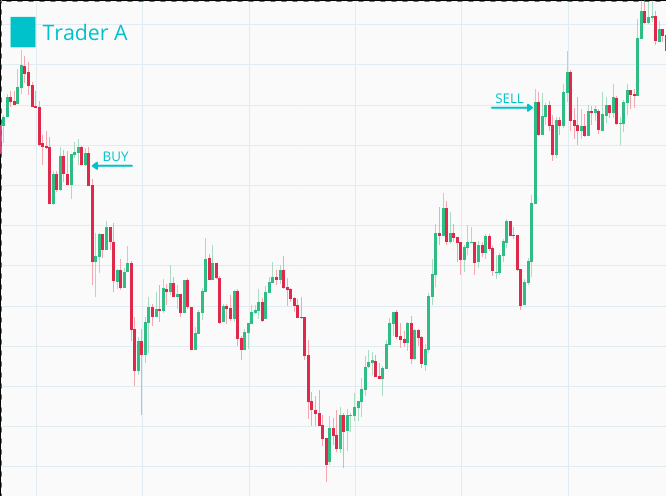
\includegraphics{images/chapter_09_01_single_trader.png}

We will implement additional trade event callback inside the \texttt{Naive.Trader} that will keep checking the price after buy order has been filled. Whenever price drops below the \texttt{buy\_order}'s \texttt{price} by \texttt{rebuy\_interval} we will notify the \texttt{Naive.Leader} to start the new \texttt{Naive.Trader} process:

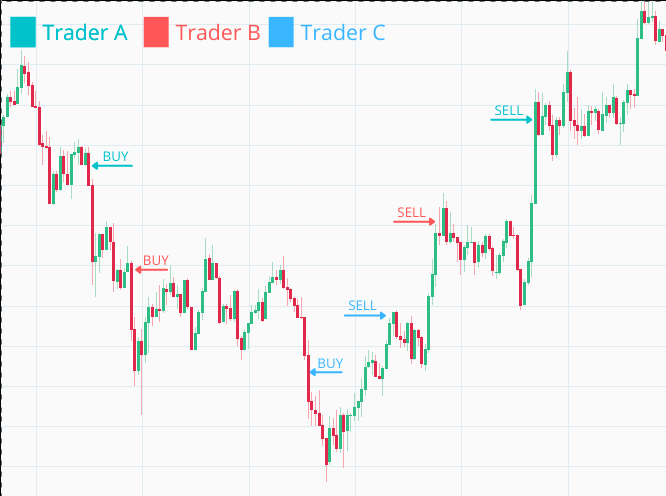
\includegraphics{images/chapter_09_02_multi_traders.png}

The \texttt{Naive.Leader} keeps track of how many \texttt{Naive.Trader}s are running and needs to honor the number of \texttt{chunks} set up in the settings (one chunk == one trader).

To stop the \texttt{Naive.Trader}s from continuously notifying about a drop in the price we will also introduce a boolean flag that will track has the \texttt{Naive.Leader} been already notified.

\hypertarget{implement-rebuy-inside-naive.trader}{%
\section{\texorpdfstring{Implement rebuy inside \texttt{Naive.Trader}}{Implement rebuy inside Naive.Trader}}\label{implement-rebuy-inside-naive.trader}}

We will start by adding the \texttt{rebuy\_interval} and the \texttt{rebuy\_notified} to trader's state:

\begin{Shaded}
\begin{Highlighting}[]
  \CommentTok{\# /apps/naive/lib/naive/trader.ex}
  \OperatorTok{...}
  \KeywordTok{defmodule} \ConstantTok{State} \KeywordTok{do}
    \OtherTok{@enforce\_keys}\NormalTok{ [}
      \VariableTok{:symbol}\NormalTok{,}
      \VariableTok{:budget}\NormalTok{,}
      \VariableTok{:buy\_down\_interval}\NormalTok{,}
      \VariableTok{:profit\_interval}\NormalTok{,}
      \VariableTok{:rebuy\_interval}\NormalTok{, }\CommentTok{\# \textless{}= add this field}
      \VariableTok{:rebuy\_notified}\NormalTok{, }\CommentTok{\# \textless{}= add this field}
      \VariableTok{:tick\_size}\NormalTok{,}
      \VariableTok{:step\_size}
\NormalTok{    ]}
    \KeywordTok{defstruct}\NormalTok{ [}
      \VariableTok{:symbol}\NormalTok{,}
      \VariableTok{:budget}\NormalTok{,}
      \VariableTok{:buy\_order}\NormalTok{,}
      \VariableTok{:sell\_order}\NormalTok{,}
      \VariableTok{:buy\_down\_interval}\NormalTok{,}
      \VariableTok{:profit\_interval}\NormalTok{,}
      \VariableTok{:rebuy\_interval}\NormalTok{, }\CommentTok{\# \textless{}= add this field}
      \VariableTok{:rebuy\_notified}\NormalTok{, }\CommentTok{\# \textless{}= add this field}
      \VariableTok{:tick\_size}\NormalTok{,}
      \VariableTok{:step\_size}
\NormalTok{    ]}
  \KeywordTok{end}
\end{Highlighting}
\end{Shaded}

Rebuy logic should be placed almost as last callback just before the one that ignores all events. We will need to retrieve the current \texttt{price} and \texttt{buy\_price} and confirm that we didn't notify the leader yet(\texttt{rebuy\_notified} flag):

\begin{Shaded}
\begin{Highlighting}[]
  \CommentTok{\# /apps/naive/lib/naive/trader.ex}
  \OperatorTok{...}
  \CommentTok{\# sell filled callback here}
  \OperatorTok{...}
  \KeywordTok{def}\NormalTok{ handle\_info(}
\NormalTok{        \%}\ConstantTok{TradeEvent}\NormalTok{\{}
          \VariableTok{price:}\NormalTok{ current\_price}
\NormalTok{        \},}
\NormalTok{        \%}\ConstantTok{State}\NormalTok{\{}
          \VariableTok{symbol:}\NormalTok{ symbol,}
          \VariableTok{buy\_order:}\NormalTok{ \%}\ConstantTok{Binance}\OperatorTok{.}\ConstantTok{OrderResponse}\NormalTok{\{}
            \VariableTok{price:}\NormalTok{ buy\_price}
\NormalTok{          \},}
          \VariableTok{rebuy\_interval:}\NormalTok{ rebuy\_interval,}
          \VariableTok{rebuy\_notified:} \ConstantTok{false}
\NormalTok{        \} }\OperatorTok{=}\NormalTok{ state}
\NormalTok{      ) }\KeywordTok{do}

  \KeywordTok{end}

  \CommentTok{\# catch all callback here}
\end{Highlighting}
\end{Shaded}

We need to calculate is the current price below the rebuy interval. If yes we will notify the leader and update the boolean flag. We will abstract calculation to separate function(for readability) that we will write below:

\begin{Shaded}
\begin{Highlighting}[]
    \CommentTok{\# /apps/naive/lib/naive/trader.ex}
    \CommentTok{\# body of the above callback}
    \ControlFlowTok{if}\NormalTok{ trigger\_rebuy?(buy\_price, current\_price, rebuy\_interval) }\KeywordTok{do}
      \ConstantTok{Logger}\OperatorTok{.}\NormalTok{info(}\StringTok{"Rebuy triggered for }\OtherTok{\#\{}\NormalTok{symbol}\OtherTok{\}}\StringTok{ trader"}\NormalTok{)}
\NormalTok{      new\_state }\OperatorTok{=}\NormalTok{ \%\{state }\OperatorTok{|} \VariableTok{rebuy\_notified:} \ConstantTok{true}\NormalTok{\}}
      \ConstantTok{Naive}\OperatorTok{.}\ConstantTok{Leader}\OperatorTok{.}\NormalTok{notify(}\VariableTok{:rebuy\_triggered}\NormalTok{, new\_state)}
\NormalTok{      \{}\VariableTok{:noreply}\NormalTok{, new\_state\}}
    \ControlFlowTok{else}
\NormalTok{      \{}\VariableTok{:noreply}\NormalTok{, state\}}
    \KeywordTok{end}
\end{Highlighting}
\end{Shaded}

As mentioned before, we will set the \texttt{rebuy\_notified} boolean flag to true and notify the leader using the \texttt{notify} function with dedicated atom.

At the bottom of the module we need to add \texttt{trigger\_rebuy?} helper function:

\begin{Shaded}
\begin{Highlighting}[]
  \CommentTok{\# /apps/naive/lib/naive/trader.ex}
  \CommentTok{\# bottom of the module}
  \KeywordTok{defp}\NormalTok{ trigger\_rebuy?(buy\_price, current\_price, rebuy\_interval) }\KeywordTok{do}
\NormalTok{    current\_price }\OperatorTok{=}\NormalTok{ D}\OperatorTok{.}\NormalTok{new(current\_price)}
\NormalTok{    buy\_price }\OperatorTok{=}\NormalTok{ D}\OperatorTok{.}\NormalTok{new(buy\_price)}

\NormalTok{    rebuy\_price }\OperatorTok{=}
\NormalTok{      D}\OperatorTok{.}\NormalTok{sub(}
\NormalTok{        buy\_price,}
\NormalTok{        D}\OperatorTok{.}\NormalTok{mult(buy\_price, rebuy\_interval)}
\NormalTok{      )}

\NormalTok{    D}\OperatorTok{.}\NormalTok{lt?(current\_price, rebuy\_price)}
  \KeywordTok{end}
\end{Highlighting}
\end{Shaded}

\hypertarget{implement-rebuy-in-the-naive.leader}{%
\section{\texorpdfstring{Implement rebuy in the \texttt{Naive.Leader}}{Implement rebuy in the Naive.Leader}}\label{implement-rebuy-in-the-naive.leader}}

Moving on to the \texttt{Naive.Leader} module, we can get update starting of the traders automatically by the leader to starting just one inside \texttt{handle\_continue}:

\begin{Shaded}
\begin{Highlighting}[]
  \CommentTok{\# /apps/naive/lib/naive/leader.ex}
  \KeywordTok{def}\NormalTok{ handle\_continue(}\VariableTok{:start\_traders}\NormalTok{, \%\{}\VariableTok{symbol:}\NormalTok{ symbol\} }\OperatorTok{=}\NormalTok{ state) }\KeywordTok{do}
    \OperatorTok{...}
\NormalTok{    traders }\OperatorTok{=}\NormalTok{ [start\_new\_trader(trader\_state)] }\CommentTok{\# \textless{}= updated part}

    \OperatorTok{...}
  \KeywordTok{end}
\end{Highlighting}
\end{Shaded}

We will need to add a new clause of \texttt{notify} function that will handle the rebuy scenario:

\begin{Shaded}
\begin{Highlighting}[]
  \CommentTok{\# /apps/naive/lib/naive/leader.ex}
  \CommentTok{\# add below current \textasciigrave{}notify\textasciigrave{} function}
  \KeywordTok{def}\NormalTok{ notify(}\VariableTok{:rebuy\_triggered}\NormalTok{, trader\_state) }\KeywordTok{do}
    \ConstantTok{GenServer}\OperatorTok{.}\NormalTok{call(}
\NormalTok{      :}\StringTok{"}\OtherTok{\#\{}\ConstantTok{\_\_MODULE\_\_}\OtherTok{\}}\StringTok{{-}}\OtherTok{\#\{}\NormalTok{trader\_state}\OperatorTok{.}\NormalTok{symbol}\OtherTok{\}}\StringTok{"}\NormalTok{,}
\NormalTok{      \{}\VariableTok{:rebuy\_triggered}\NormalTok{, trader\_state\}}
\NormalTok{    )}
  \KeywordTok{end}
\end{Highlighting}
\end{Shaded}

We need to add a new \texttt{handle\_call} function that will start new traders only when there are still chunks available(enforce the maximum number of parallel
traders) - let's start with a header:

\begin{Shaded}
\begin{Highlighting}[]
  \CommentTok{\# /apps/naive/lib/naive/leader.ex}
  \CommentTok{\# place this one after :update\_trader\_state handle\_call}
  \KeywordTok{def}\NormalTok{ handle\_call(}
\NormalTok{        \{}\VariableTok{:rebuy\_triggered}\NormalTok{, new\_trader\_state\},}
\NormalTok{        \{trader\_pid, \_\},}
\NormalTok{        \%\{}\VariableTok{traders:}\NormalTok{ traders, }\VariableTok{symbol:}\NormalTok{ symbol, }\VariableTok{settings:}\NormalTok{ settings\} }\OperatorTok{=}\NormalTok{ state}
\NormalTok{      ) }\KeywordTok{do}

  \KeywordTok{end}
\end{Highlighting}
\end{Shaded}

There are few important details to make note of:
- we need trader's pid to be able to find it details inside the list of traders
- we need settings to cofirm number of chunks to be able to limit maximum number of parallel traders

Moving on to the body of our callback. As with other ones, we will check can we find trader inside list of traders and based on that we will either start another one(if we didn't reach the limit of chunks) or ignore it:

\begin{Shaded}
\begin{Highlighting}[]
    \CommentTok{\# /apps/naive/lib/naive/leader.ex}
    \CommentTok{\# body of our callback}
    \KeywordTok{case} \ConstantTok{Enum}\OperatorTok{.}\NormalTok{find\_index(traders, }\OperatorTok{\&}\NormalTok{(}\OperatorTok{\&}\DecValTok{1}\OperatorTok{.}\NormalTok{pid }\OperatorTok{==}\NormalTok{ trader\_pid)) }\KeywordTok{do}
      \ConstantTok{nil} \OperatorTok{{-}\textgreater{}}
        \ConstantTok{Logger}\OperatorTok{.}\NormalTok{warn(}\StringTok{"Rebuy triggered by trader that leader is not aware of"}\NormalTok{)}
\NormalTok{        \{}\VariableTok{:reply}\NormalTok{, }\VariableTok{:ok}\NormalTok{, state\}}

\NormalTok{      index }\OperatorTok{{-}\textgreater{}}
\NormalTok{        old\_trader\_data }\OperatorTok{=} \ConstantTok{Enum}\OperatorTok{.}\NormalTok{at(traders, index)}
\NormalTok{        new\_trader\_data }\OperatorTok{=}\NormalTok{ \%\{old\_trader\_data }\OperatorTok{|} \VariableTok{:state} \OperatorTok{=\textgreater{}}\NormalTok{ new\_trader\_state\}}
\NormalTok{        updated\_traders }\OperatorTok{=} \ConstantTok{List}\OperatorTok{.}\NormalTok{replace\_at(traders, index, new\_trader\_data)}

\NormalTok{        updated\_traders }\OperatorTok{=}
          \ControlFlowTok{if}\NormalTok{ settings}\OperatorTok{.}\NormalTok{chunks }\OperatorTok{==}\NormalTok{ length(traders) }\KeywordTok{do}
            \ConstantTok{Logger}\OperatorTok{.}\NormalTok{info(}\StringTok{"All traders already started for }\OtherTok{\#\{}\NormalTok{symbol}\OtherTok{\}}\StringTok{"}\NormalTok{)}
\NormalTok{            updated\_traders}
          \ControlFlowTok{else}
            \ConstantTok{Logger}\OperatorTok{.}\NormalTok{info(}\StringTok{"Starting new trader for }\OtherTok{\#\{}\NormalTok{symbol}\OtherTok{\}}\StringTok{"}\NormalTok{)}
\NormalTok{            [start\_new\_trader(fresh\_trader\_state(settings)) }\OperatorTok{|}\NormalTok{ updated\_traders]}
          \KeywordTok{end}

\NormalTok{        \{}\VariableTok{:reply}\NormalTok{, }\VariableTok{:ok}\NormalTok{, \%\{state }\OperatorTok{|} \VariableTok{:traders} \OperatorTok{=\textgreater{}}\NormalTok{ updated\_traders\}\}}
    \KeywordTok{end}
\end{Highlighting}
\end{Shaded}

In above code we need to remember to update the state of the trader that triggered the rebuy inside the \texttt{traders} list as well as add state of a new trader to that list.

As with other setting we will hardcode the \texttt{rebuy\_interval}(inside the \texttt{fetch\_symbol\_settings} function) and assign them to
trader's state(inside the \texttt{fresh\_trader\_state} function):

\begin{Shaded}
\begin{Highlighting}[]
  \CommentTok{\# /apps/naive/lib/naive/leader.ex}
  \KeywordTok{defp}\NormalTok{ fresh\_trader\_state(settings) }\KeywordTok{do}
\NormalTok{    \%\{}
\NormalTok{      struct(}\ConstantTok{Trader}\OperatorTok{.}\ConstantTok{State}\NormalTok{, settings)}
      \OperatorTok{|} \VariableTok{budget:}\NormalTok{ D}\OperatorTok{.}\NormalTok{div(settings}\OperatorTok{.}\NormalTok{budget, settings}\OperatorTok{.}\NormalTok{chunks),}
        \VariableTok{rebuy\_notified:} \ConstantTok{false} \CommentTok{\# \textless{}= add this line}
\NormalTok{    \}}
  \KeywordTok{end}

  \KeywordTok{defp}\NormalTok{ fetch\_symbol\_settings(symbol) }\KeywordTok{do}
    \OperatorTok{...}

    \ConstantTok{Map}\OperatorTok{.}\NormalTok{merge(}
\NormalTok{      \%\{}
        \OperatorTok{...}
        \VariableTok{chunks:} \DecValTok{5}\NormalTok{, }\CommentTok{\# \textless{}= update to 5 parallel traders max}
        \VariableTok{budget:} \ConstantTok{Decimal}\OperatorTok{.}\NormalTok{new(}\StringTok{"100"}\NormalTok{), }\CommentTok{\# \textless{}= update this line}
        \OperatorTok{...}
        \VariableTok{profit\_interval:} \ConstantTok{Decimal}\OperatorTok{.}\NormalTok{new(}\StringTok{"{-}0.0012"}\NormalTok{),}
        \VariableTok{rebuy\_interval:} \ConstantTok{Decimal}\OperatorTok{.}\NormalTok{new(}\StringTok{"0.001"}\NormalTok{) }\CommentTok{\# \textless{}= add this line}
\NormalTok{      \},}
\NormalTok{      symbol\_filters}
\NormalTok{    )}
  \KeywordTok{end}
\end{Highlighting}
\end{Shaded}

We also update the \texttt{chunks} and the \texttt{budget} to allow our strategy to start up to 5 parallel traders with a budget of 20 USDT each(100/5) as Binance has minimal order requirement at about \$15(when using the \texttt{BinanceMock} this doesn't really matter).

\hypertarget{improve-logs-by-assigning-ids-to-traders}{%
\section{Improve logs by assigning ids to traders}\label{improve-logs-by-assigning-ids-to-traders}}

The final change will be to add an \texttt{id} to trader's state so we can use it inside log messages to give us meaningful data about what's going on(otherwise we won't be able to tell which message was logged by which trader).

First let's add the \texttt{id} into the \texttt{Naive.Leader}'s fresh\_trader\_state as it will be defined per trader:

\begin{Shaded}
\begin{Highlighting}[]
  \CommentTok{\# /apps/naive/lib/naive/leader.ex}
  \KeywordTok{defp}\NormalTok{ fresh\_trader\_state(settings) }\KeywordTok{do}
\NormalTok{    \%\{}
\NormalTok{      struct(}\ConstantTok{Trader}\OperatorTok{.}\ConstantTok{State}\NormalTok{, settings)}
      \OperatorTok{|} \VariableTok{id:} \VariableTok{:os}\OperatorTok{.}\NormalTok{system\_time(}\VariableTok{:millisecond}\NormalTok{), }\CommentTok{\# \textless{}= add this line}
        \VariableTok{budget:}\NormalTok{ D}\OperatorTok{.}\NormalTok{div(settings}\OperatorTok{.}\NormalTok{budget, settings}\OperatorTok{.}\NormalTok{chunks),}
        \VariableTok{rebuy\_notified:} \ConstantTok{false}
\NormalTok{    \}}
  \KeywordTok{end}
\end{Highlighting}
\end{Shaded}

Now we can move on to the \texttt{Naive.Trader} and add it to the \texttt{\%State\{\}} struct as well as we will modify every callback to include that id inside log messages:

\begin{Shaded}
\begin{Highlighting}[]
  \CommentTok{\# /apps/naive/lib/naive/trader.ex}
  \KeywordTok{defmodule} \ConstantTok{State} \KeywordTok{do}
    \OtherTok{@enforce\_keys}\NormalTok{ [}
      \VariableTok{:id}\NormalTok{,}
      \OperatorTok{...}
\NormalTok{    ]}
    \KeywordTok{defstruct}\NormalTok{ [}
      \VariableTok{:id}\NormalTok{,}
      \OperatorTok{...}
\NormalTok{    ]}
  \KeywordTok{end}

  \OperatorTok{...}

  \KeywordTok{def}\NormalTok{ init(\%}\ConstantTok{State}\NormalTok{\{}\VariableTok{id:}\NormalTok{ id, }\VariableTok{symbol:}\NormalTok{ symbol\} }\OperatorTok{=}\NormalTok{ state) }\KeywordTok{do}
    \OperatorTok{...}

    \ConstantTok{Logger}\OperatorTok{.}\NormalTok{info(}\StringTok{"Initializing new trader(}\OtherTok{\#\{}\NormalTok{id}\OtherTok{\}}\StringTok{) for }\OtherTok{\#\{}\NormalTok{symbol}\OtherTok{\}}\StringTok{"}\NormalTok{)}

    \OperatorTok{...}
  \KeywordTok{end}

  \KeywordTok{def}\NormalTok{ handle\_info(}
\NormalTok{        \%}\ConstantTok{TradeEvent}\NormalTok{\{}\VariableTok{price:}\NormalTok{ price\},}
\NormalTok{        \%}\ConstantTok{State}\NormalTok{\{}
          \VariableTok{id:}\NormalTok{ id,}
          \OperatorTok{...}
\NormalTok{        \} }\OperatorTok{=}\NormalTok{ state}
\NormalTok{      ) }\KeywordTok{do}
    \OperatorTok{...}

    \ConstantTok{Logger}\OperatorTok{.}\NormalTok{info(}
      \StringTok{"The trader(}\OtherTok{\#\{}\NormalTok{id}\OtherTok{\}}\StringTok{) is placing a BUY order "} \OperatorTok{\textless{}\textgreater{}}
        \StringTok{"for }\OtherTok{\#\{}\NormalTok{symbol}\OtherTok{\}}\StringTok{ @ }\OtherTok{\#\{}\NormalTok{price}\OtherTok{\}}\StringTok{, quantity: }\OtherTok{\#\{}\NormalTok{quantity}\OtherTok{\}}\StringTok{"}
\NormalTok{    )}

    \OperatorTok{...}
  \KeywordTok{end}

  \KeywordTok{def}\NormalTok{ handle\_info(}
\NormalTok{        \%}\ConstantTok{TradeEvent}\NormalTok{\{}
          \VariableTok{buyer\_order\_id:}\NormalTok{ order\_id}
\NormalTok{        \},}
\NormalTok{        \%}\ConstantTok{State}\NormalTok{\{}
          \VariableTok{id:}\NormalTok{ id,}
          \OperatorTok{...}
\NormalTok{        \} }\OperatorTok{=}\NormalTok{ state}
\NormalTok{      ) }\KeywordTok{do}
    \OperatorTok{...}
        \ConstantTok{Logger}\OperatorTok{.}\NormalTok{info(}
          \StringTok{"The trader(}\OtherTok{\#\{}\NormalTok{id}\OtherTok{\}}\StringTok{) is placing a SELL order for "} \OperatorTok{\textless{}\textgreater{}}
            \StringTok{"}\OtherTok{\#\{}\NormalTok{symbol}\OtherTok{\}}\StringTok{ @ }\OtherTok{\#\{}\NormalTok{sell\_price}\OtherTok{\}}\StringTok{, quantity: }\OtherTok{\#\{}\NormalTok{quantity}\OtherTok{\}}\StringTok{."}
\NormalTok{        )}
        \OperatorTok{...}
        \ConstantTok{Logger}\OperatorTok{.}\NormalTok{info(}\StringTok{"Trader\textquotesingle{}s(}\OtherTok{\#\{}\NormalTok{id}\OtherTok{\}}\StringTok{ }\OtherTok{\#\{}\NormalTok{symbol}\OtherTok{\}}\StringTok{ BUY order got partially filled"}\NormalTok{)}
        \OperatorTok{...}
  \KeywordTok{end}

  \KeywordTok{def}\NormalTok{ handle\_info(}
\NormalTok{        \%}\ConstantTok{TradeEvent}\NormalTok{\{}
          \VariableTok{seller\_order\_id:}\NormalTok{ order\_id}
\NormalTok{        \},}
\NormalTok{        \%}\ConstantTok{State}\NormalTok{\{}
          \VariableTok{id:}\NormalTok{ id,}
          \OperatorTok{...}
\NormalTok{        \} }\OperatorTok{=}\NormalTok{ state}
\NormalTok{      ) }\KeywordTok{do}
    \OperatorTok{...}
      \ConstantTok{Logger}\OperatorTok{.}\NormalTok{info(}\StringTok{"Trader(}\OtherTok{\#\{}\NormalTok{id}\OtherTok{\}}\StringTok{) finished trade cycle for }\OtherTok{\#\{}\NormalTok{symbol}\OtherTok{\}}\StringTok{"}\NormalTok{)}
      \OperatorTok{...}
      \ConstantTok{Logger}\OperatorTok{.}\NormalTok{info(}\StringTok{"Trader\textquotesingle{}s(}\OtherTok{\#\{}\NormalTok{id}\OtherTok{\}}\StringTok{ }\OtherTok{\#\{}\NormalTok{symbol}\OtherTok{\}}\StringTok{ SELL order got partially filled"}\NormalTok{)      }\OperatorTok{...}
  \KeywordTok{end}

  \KeywordTok{def}\NormalTok{ handle\_info(}
\NormalTok{        \%}\ConstantTok{TradeEvent}\NormalTok{\{}
          \VariableTok{price:}\NormalTok{ current\_price}
\NormalTok{        \},}
\NormalTok{        \%}\ConstantTok{State}\NormalTok{\{}
          \VariableTok{id:}\NormalTok{ id,}
          \OperatorTok{...}
\NormalTok{        \} }\OperatorTok{=}\NormalTok{ state}
\NormalTok{      ) }\KeywordTok{do}
      \OperatorTok{...}
      \ConstantTok{Logger}\OperatorTok{.}\NormalTok{info(}\StringTok{"Rebuy triggered for }\OtherTok{\#\{}\NormalTok{symbol}\OtherTok{\}}\StringTok{ by the trader(}\OtherTok{\#\{}\NormalTok{id}\OtherTok{\}}\StringTok{)"}\NormalTok{)}
      \OperatorTok{...}
  \KeywordTok{end}
\end{Highlighting}
\end{Shaded}

That finishes the implementation part - we should now be able to test the implementation and see dynamically growing number of traders for our strategy based on price movement.

\hypertarget{test-the-implementation-2}{%
\section{Test the implementation}\label{test-the-implementation-2}}

Let's start an iEx the session and open the \texttt{:observer}(inside go to ``Applications'' tab and click on \texttt{naive} from the list of the left) so we will be able to see how the number of traders is growing as well as PIDs are changing which means that they are finishing the full trades:

\begin{Shaded}
\begin{Highlighting}[]
\ExtensionTok{$}\NormalTok{ iex }\AttributeTok{{-}S}\NormalTok{ mix}
\ExtensionTok{...}
\ExtensionTok{iex}\ErrorTok{(}\ExtensionTok{1}\KeywordTok{)}\OperatorTok{\textgreater{}}\NormalTok{ :observer.start}\KeywordTok{()}
\ExtensionTok{...}
\ExtensionTok{iex}\ErrorTok{(}\ExtensionTok{2}\KeywordTok{)}\OperatorTok{\textgreater{}}\NormalTok{ Naive.start\_trading}\KeywordTok{(}\StringTok{"HNTUSDT"}\KeywordTok{)}
\ExtensionTok{10:22:05.018}\NormalTok{ [info]  The trader}\ErrorTok{(}\ExtensionTok{1616754009963}\KeywordTok{)} \ExtensionTok{is}\NormalTok{ placing a BUY order for HNTUSDT @ 8.175, quantity: 2.446}
\ExtensionTok{10:22:11.665}\NormalTok{ [info]  Rebuy triggered for HNTUSDT by the trader}\ErrorTok{(}\ExtensionTok{1616754009963}\KeywordTok{)}
\ExtensionTok{10:22:11.665}\NormalTok{ [info]  Starting new trader for HNTUSDT}
\ExtensionTok{10:22:11.665}\NormalTok{ [info]  Initializing new trader}\ErrorTok{(}\ExtensionTok{1616754131665}\KeywordTok{)} \ControlFlowTok{for}\NormalTok{ HNTUSDT}
\ExtensionTok{10:22:11.665}\NormalTok{ [info]  The trader}\ErrorTok{(}\ExtensionTok{1616754009963}\KeywordTok{)} \ExtensionTok{is}\NormalTok{ placing a SELL order for HNTUSDT @ 8.181, quantity: 2.446.}
\ExtensionTok{10:22:11.665}\NormalTok{ [info]  The trader}\ErrorTok{(}\ExtensionTok{1616754131665}\KeywordTok{)} \ExtensionTok{is}\NormalTok{ placing a BUY order for HNTUSDT @ 8.157, quantity: 2.451}
\ExtensionTok{10:22:58.339}\NormalTok{ [info]  Trader}\ErrorTok{(}\ExtensionTok{1616754009963}\KeywordTok{)} \ExtensionTok{finished}\NormalTok{ trade cycle for HNTUSDT}
\ExtensionTok{10:22:58.339}\NormalTok{ [info]  HNTUSDT trader finished trade }\AttributeTok{{-}}\NormalTok{ restarting}
\ExtensionTok{10:22:58.339}\NormalTok{ [info]  Initializing new trader}\ErrorTok{(}\ExtensionTok{1616754178339}\KeywordTok{)} \ControlFlowTok{for}\NormalTok{ HNTUSDT}
\ExtensionTok{10:22:58.339}\NormalTok{ [info]  The trader}\ErrorTok{(}\ExtensionTok{1616754178339}\KeywordTok{)} \ExtensionTok{is}\NormalTok{ placing a BUY order for HNTUSDT @ 8.212, quantity: 2.435}
\ExtensionTok{10:23:13.232}\NormalTok{ [info]  Rebuy triggered for HNTUSDT by the trader}\ErrorTok{(}\ExtensionTok{1616754178339}\KeywordTok{)}
\ExtensionTok{10:23:13.232}\NormalTok{ [info]  Starting new trader for HNTUSDT}
\ExtensionTok{10:23:13.232}\NormalTok{ [info]  Initializing new trader}\ErrorTok{(}\ExtensionTok{1616754193232}\KeywordTok{)} \ControlFlowTok{for}\NormalTok{ HNTUSDT}
\ExtensionTok{10:23:13.232}\NormalTok{ [info]  The trader}\ErrorTok{(}\ExtensionTok{1616754178339}\KeywordTok{)} \ExtensionTok{is}\NormalTok{ placing a SELL order for HNTUSDT @ 8.218, quantity: 2.435.}
\ExtensionTok{10:23:31.120}\NormalTok{ [info]  The trader}\ErrorTok{(}\ExtensionTok{1616754193232}\KeywordTok{)} \ExtensionTok{is}\NormalTok{ placing a BUY order for HNTUSDT @ 8.194, quantity: 2.44}
\ExtensionTok{10:23:31.121}\NormalTok{ [info]  Trader}\ErrorTok{(}\ExtensionTok{1616754178339}\KeywordTok{)} \ExtensionTok{finished}\NormalTok{ trade cycle for HNTUSDT}
\ExtensionTok{10:23:31.122}\NormalTok{ [info]  HNTUSDT trader finished trade }\AttributeTok{{-}}\NormalTok{ restarting}
\ExtensionTok{10:23:31.122}\NormalTok{ [info]  Initializing new trader}\ErrorTok{(}\ExtensionTok{1616754211122}\KeywordTok{)} \ControlFlowTok{for}\NormalTok{ HNTUSDT}
\ExtensionTok{10:24:31.891}\NormalTok{ [info]  The trader}\ErrorTok{(}\ExtensionTok{1616754211122}\KeywordTok{)} \ExtensionTok{is}\NormalTok{ placing a BUY order for HNTUSDT @ 8.198, quantity: 2.439}
\ExtensionTok{10:25:24.155}\NormalTok{ [info]  The trader}\ErrorTok{(}\ExtensionTok{1616754211122}\KeywordTok{)} \ExtensionTok{is}\NormalTok{ placing a SELL order for HNTUSDT @ 8.204, quantity: 2.439.}
\ExtensionTok{10:25:24.155}\NormalTok{ [info]  The trader}\ErrorTok{(}\ExtensionTok{1616754193232}\KeywordTok{)} \ExtensionTok{is}\NormalTok{ placing a SELL order for HNTUSDT @ 8.2, quantity: 2.44.}
\ExtensionTok{10:25:24.155}\NormalTok{ [info]  Rebuy triggered for HNTUSDT by the trader}\ErrorTok{(}\ExtensionTok{1616754211122}\KeywordTok{)}
\ExtensionTok{10:25:24.155}\NormalTok{ [info]  Starting new trader for HNTUSDT}
\ExtensionTok{10:25:24.156}\NormalTok{ [info]  Initializing new trader}\ErrorTok{(}\ExtensionTok{1616754324155}\KeywordTok{)} \ControlFlowTok{for}\NormalTok{ HNTUSDT}
\ExtensionTok{10:25:24.156}\NormalTok{ [info]  Rebuy triggered for HNTUSDT by the trader}\ErrorTok{(}\ExtensionTok{1616754193232}\KeywordTok{)}
\ExtensionTok{10:25:24.156}\NormalTok{ [info]  The trader}\ErrorTok{(}\ExtensionTok{1616754324155}\KeywordTok{)} \ExtensionTok{is}\NormalTok{ placing a BUY order for HNTUSDT @ 8.183, quantity: 2.444}
\ExtensionTok{10:25:24.156}\NormalTok{ [info]  Starting new trader for HNTUSDT}
\ExtensionTok{10:25:24.156}\NormalTok{ [info]  Initializing new trader}\ErrorTok{(}\ExtensionTok{1616754324156}\KeywordTok{)} \ControlFlowTok{for}\NormalTok{ HNTUSDT }
\ExtensionTok{10:25:24.156}\NormalTok{ [info]  The trader}\ErrorTok{(}\ExtensionTok{1616754324156}\KeywordTok{)} \ExtensionTok{is}\NormalTok{ placing a BUY order for HNTUSDT @ 8.176, quantity: 2.446}
\ExtensionTok{10:25:24.156}\NormalTok{ [info]  The trader}\ErrorTok{(}\ExtensionTok{1616754324155}\KeywordTok{)} \ExtensionTok{is}\NormalTok{ placing a SELL order for HNTUSDT @ 8.189, quantity: 2.444.}
\ExtensionTok{10:25:37.527}\NormalTok{ [info]  Trader}\ErrorTok{(}\ExtensionTok{1616754324155}\KeywordTok{)} \ExtensionTok{finished}\NormalTok{ trade cycle for HNTUSDT}
\ExtensionTok{10:25:37.528}\NormalTok{ [info]  HNTUSDT trader finished trade }\AttributeTok{{-}}\NormalTok{ restarting}
\ExtensionTok{10:25:37.528}\NormalTok{ [info]  Initializing new trader}\ErrorTok{(}\ExtensionTok{1616754337528}\KeywordTok{)} \ControlFlowTok{for}\NormalTok{ HNTUSDT}
\ExtensionTok{10:25:37.528}\NormalTok{ [info]  The trader}\ErrorTok{(}\ExtensionTok{1616754337528}\KeywordTok{)} \ExtensionTok{is}\NormalTok{ placing a BUY order for HNTUSDT @ 8.192, quantity: 2.441}
\ExtensionTok{10:25:37.530}\NormalTok{ [info]  Trader}\ErrorTok{(}\ExtensionTok{1616754211122}\KeywordTok{)} \ExtensionTok{finished}\NormalTok{ trade cycle for HNTUSDT}
\ExtensionTok{10:25:37.530}\NormalTok{ [info]  Trader}\ErrorTok{(}\ExtensionTok{1616754193232}\KeywordTok{)} \ExtensionTok{finished}\NormalTok{ trade cycle for HNTUSDT}
\ExtensionTok{10:25:37.530}\NormalTok{ [info]  HNTUSDT trader finished trade }\AttributeTok{{-}}\NormalTok{ restarting}
\ExtensionTok{10:25:37.530}\NormalTok{ [info]  Initializing new trader}\ErrorTok{(}\ExtensionTok{1616754337530}\KeywordTok{)} \ControlFlowTok{for}\NormalTok{ HNTUSDT}
\ExtensionTok{10:25:37.530}\NormalTok{ [info]  HNTUSDT trader finished trade }\AttributeTok{{-}}\NormalTok{ restarting}
\ExtensionTok{10:25:37.530}\NormalTok{ [info]  Initializing new trader}\ErrorTok{(}\ExtensionTok{1616754337530}\KeywordTok{)} \ControlFlowTok{for}\NormalTok{ HNTUSDT}
\ExtensionTok{10:25:40.015}\NormalTok{ [info]  Rebuy triggered for HNTUSDT by the trader}\ErrorTok{(}\ExtensionTok{1616754337528}\KeywordTok{)}
\ExtensionTok{10:25:40.015}\NormalTok{ [info]  The trader}\ErrorTok{(}\ExtensionTok{1616754337530}\KeywordTok{)} \ExtensionTok{is}\NormalTok{ placing a BUY order for HNTUSDT @ 8.179, quantity: 2.445}
\ExtensionTok{10:25:40.015}\NormalTok{ [info]  All traders already started for HNTUSDT}
\end{Highlighting}
\end{Shaded}

And our observer shows the following:

\begin{figure}
\centering
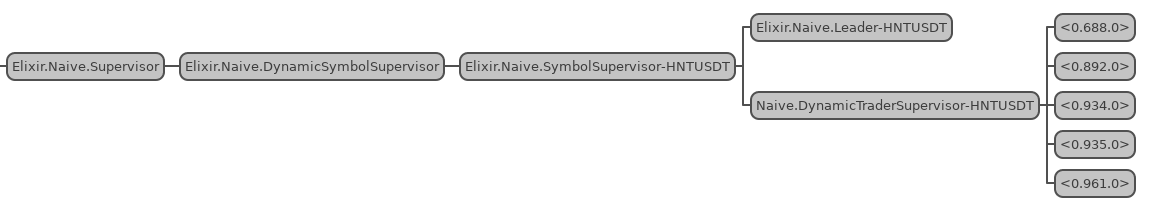
\includegraphics{images/chapter_09_supervision_tree.png}
\caption{Observer shows 5 parallel traders}
\end{figure}

We can clearly see that our strategy dynamically scaled from 1 to 5 parallel traders and they were going through different trading steps without any problems - I think that's really cool to see and it wasn't difficult to achieve in Elixir.

{[}Note{]} Please remember to run \texttt{mix\ format} to keep things nice and tidy.

Source code for this chapter can be found at \href{https://github.com/frathon/create-a-cryptocurrency-trading-bot-in-elixir-source-code/tree/chapter_09}{Github}

\hypertarget{fine-tune-trading-strategy-per-symbol}{%
\chapter{Fine-tune trading strategy per symbol}\label{fine-tune-trading-strategy-per-symbol}}

\hypertarget{objectives-9}{%
\section{Objectives}\label{objectives-9}}

\begin{itemize}
\tightlist
\item
  describe and design the required functionality
\item
  add docker to project
\item
  set up \texttt{ecto} inside the \texttt{naive} app
\item
  create and migrate the DB
\item
  seed symbols' settings
\item
  update the \texttt{Naive.Leader} to fetch settings
\end{itemize}

\hypertarget{describe-and-design-the-required-functionality-1}{%
\section{Describe and design the required functionality}\label{describe-and-design-the-required-functionality-1}}

At this moment the settings of our naive strategy are hardcoded inside the \texttt{Naive.Leader}:

\begin{Shaded}
\begin{Highlighting}[]
  \CommentTok{\# /apps/naive/lib/naive/leader.ex}
  \OperatorTok{...}
  \KeywordTok{defp}\NormalTok{ fetch\_symbol\_settings(symbol) }\KeywordTok{do}
\NormalTok{    symbol\_filters }\OperatorTok{=}\NormalTok{ fetch\_symbol\_filters(symbol)}

    \ConstantTok{Map}\OperatorTok{.}\NormalTok{merge(}
\NormalTok{      \%\{}
        \VariableTok{symbol:}\NormalTok{ symbol,                           }\CommentTok{\# \textless{}=}
        \VariableTok{chunks:} \DecValTok{5}\NormalTok{,                                }\CommentTok{\# \textless{}=}
        \VariableTok{budget:} \ConstantTok{Decimal}\OperatorTok{.}\NormalTok{new(}\StringTok{"100"}\NormalTok{),               }\CommentTok{\# \textless{}=}
        \VariableTok{buy\_down\_interval:} \ConstantTok{Decimal}\OperatorTok{.}\NormalTok{new(}\StringTok{"0.0001"}\NormalTok{), }\CommentTok{\# \textless{}= all of those settings}
        \CommentTok{\# {-}0.12\% for quick testing                \# \textless{}=}
        \VariableTok{profit\_interval:} \ConstantTok{Decimal}\OperatorTok{.}\NormalTok{new(}\StringTok{"{-}0.0012"}\NormalTok{),  }\CommentTok{\# \textless{}=}
        \VariableTok{rebuy\_interval:} \ConstantTok{Decimal}\OperatorTok{.}\NormalTok{new(}\StringTok{"0.001"}\NormalTok{)      }\CommentTok{\# \textless{}=}
\NormalTok{      \},}
\NormalTok{      symbol\_filters}
\NormalTok{    )}
  \KeywordTok{end}
  \OperatorTok{...}
\end{Highlighting}
\end{Shaded}

The problem about those is that they are hardcoded and there's no flexibility to define them per symbol at the moment.

In this chapter, we will move them out from this file into the Postgres database.

\hypertarget{add-docker-to-project}{%
\section{Add docker to project}\label{add-docker-to-project}}

The requirements for this section are \texttt{docker} and \texttt{docker-compose} installed in your system.

Inside the main directory of our project create a new file called \texttt{docker-compose.yml} and fill it with below details:

\begin{verbatim}
# /docker-compose.yml
version: "3.2"
services:
  db:
    image: postgres:latest
    restart: always
    environment:
      POSTGRES_PASSWORD: "postgres"
    ports:
      - 5432:5432
    volumes:
      - ../postgres-data:/var/lib/postgresql/data
\end{verbatim}

If you are new to docker here's the gist of what the above will do:
- it will start a single service called ``db''
- ``db'' service will use the \texttt{latest} version of the \texttt{postgres} (image) inside the docker container (\texttt{latest} version as tagged per \url{https://hub.docker.com/_/postgres/})
- we map TCP port 5432 in the container to port 5432 on the Docker host(format container\_port:hosts\_port)
- we set up environmental variable inside the docker container that will be used by the Postgres app as a password for the default (\texttt{postgres}) user
- \texttt{volumes} option maps the directory from inside of the container to the host. This way we will keep the state of the database between restarts.

We can now start the service using \texttt{docker-compose}:

\begin{Shaded}
\begin{Highlighting}[]
\ExtensionTok{$}\NormalTok{ docker{-}compose up }\AttributeTok{{-}d}
\ExtensionTok{Creating}\NormalTok{ hedgehog\_db\_1 ... done}
\end{Highlighting}
\end{Shaded}

To validate that it works we can run:

\begin{Shaded}
\begin{Highlighting}[]
\ExtensionTok{$}\NormalTok{ docker ps }\AttributeTok{{-}a}
\ExtensionTok{CONTAINER}\NormalTok{ ID   IMAGE             COMMAND                  CREATED         STATUS         PORTS                    NAMES}
\ExtensionTok{98558827b80b}\NormalTok{   postgres:latest   }\StringTok{"docker{-}entrypoint.s…"}\NormalTok{   4 seconds ago   Up 4 seconds   0.0.0.0:5432{-}}\OperatorTok{\textgreater{}}\NormalTok{5432/tcp   hedgehog\_db\_1}
\end{Highlighting}
\end{Shaded}

\hypertarget{set-up-ecto-inside-the-naive-app}{%
\section{\texorpdfstring{Set up \texttt{ecto} inside the \texttt{naive} app}{Set up ecto inside the naive app}}\label{set-up-ecto-inside-the-naive-app}}

Let's start by adding database access to the \texttt{naive} application. The first step is to add the \href{https://github.com/elixir-ecto/ecto}{Ecto} module together with the \href{https://github.com/elixir-ecto/postgrex}{Postgrex} ecto's driver package to the \texttt{deps} function inside the \texttt{mix.exs} file. As we are going to use Enums inside Postgres, we need to add the \href{https://github.com/gjaldon/ecto_enum}{EctoEnum} module as well:

\begin{Shaded}
\begin{Highlighting}[]
  \CommentTok{\# /apps/naive/mix.exs}
  \KeywordTok{defp}\NormalTok{ deps }\KeywordTok{do}
\NormalTok{    [}
\NormalTok{      \{}\VariableTok{:binance}\NormalTok{, }\StringTok{"\textasciitilde{}\textgreater{} 0.7.1"}\NormalTok{\},}
\NormalTok{      \{}\VariableTok{:binance\_mock}\NormalTok{, }\VariableTok{in\_umbrella:} \ConstantTok{true}\NormalTok{\},}
\NormalTok{      \{}\VariableTok{:decimal}\NormalTok{, }\StringTok{"\textasciitilde{}\textgreater{} 2.0"}\NormalTok{\},}
\NormalTok{      \{}\VariableTok{:ecto\_sql}\NormalTok{, }\StringTok{"\textasciitilde{}\textgreater{} 3.0"}\NormalTok{\},     }\CommentTok{\# \textless{}= New line}
\NormalTok{      \{}\VariableTok{:ecto\_enum}\NormalTok{, }\StringTok{"\textasciitilde{}\textgreater{} 1.4"}\NormalTok{\},    }\CommentTok{\# \textless{}= New line}
\NormalTok{      \{}\VariableTok{:phoenix\_pubsub}\NormalTok{, }\StringTok{"\textasciitilde{}\textgreater{} 2.0"}\NormalTok{\},}
\NormalTok{      \{}\VariableTok{:postgrex}\NormalTok{, }\StringTok{"\textgreater{}= 0.0.0"}\NormalTok{\},   }\CommentTok{\# \textless{}= New line}
\NormalTok{      \{}\VariableTok{:streamer}\NormalTok{, }\VariableTok{in\_umbrella:} \ConstantTok{true}\NormalTok{\}}
\NormalTok{    ]}
  \KeywordTok{end}
\end{Highlighting}
\end{Shaded}

Remember about installing those deps using:

\begin{Shaded}
\begin{Highlighting}[]
\ExtensionTok{$}\NormalTok{ mix deps.get}
\end{Highlighting}
\end{Shaded}

We can now use the ecto generator to add an the ecto repository to the Naive application:

\begin{Shaded}
\begin{Highlighting}[]
\ExtensionTok{$}\NormalTok{ cd apps/naive}
\ExtensionTok{$}\NormalTok{ mix ecto.gen.repo }\AttributeTok{{-}r}\NormalTok{ Naive.Repo}
\ExtensionTok{*}\NormalTok{ creating lib/naive}
\ExtensionTok{*}\NormalTok{ creating lib/naive/repo.ex}
\ExtensionTok{*}\NormalTok{ updating ../../config/config.exs}
\ExtensionTok{Don}\StringTok{\textquotesingle{}t forget to add your new repo to your supervision tree}
\StringTok{(typically in lib/naive/application.ex):}

\StringTok{    \{Naive.Repo, []\}}

\StringTok{And to add it to the list of Ecto repositories in your}
\StringTok{configuration files (so Ecto tasks work as expected):}

\StringTok{    config :naive,}
\StringTok{      ecto\_repos: [Naive.Repo]}
\end{Highlighting}
\end{Shaded}

Back to the IDE, the generator updated our \texttt{config/config.exs} file with the default access details to the database, we need to modify them to point to our Postgres docker instance as well as add a list of ecto repositories for our naive app (as per instruction above):

\begin{Shaded}
\begin{Highlighting}[]
\CommentTok{\# /config/config.exs}
\NormalTok{config }\VariableTok{:naive}\NormalTok{,                }\CommentTok{\# \textless{}= added line}
  \VariableTok{ecto\_repos:}\NormalTok{ [}\ConstantTok{Naive}\OperatorTok{.}\ConstantTok{Repo}\NormalTok{],   }\CommentTok{\# \textless{}= added line}
  \VariableTok{binance\_client:} \ConstantTok{BinanceMock} \CommentTok{\# \textless{}= merged from existing config}

\NormalTok{config }\VariableTok{:naive}\NormalTok{, }\ConstantTok{Naive}\OperatorTok{.}\ConstantTok{Repo}\NormalTok{,}
  \VariableTok{database:} \StringTok{"naive"}\NormalTok{,    }\CommentTok{\# \textless{}= updated}
  \VariableTok{username:} \StringTok{"postgres"}\NormalTok{, }\CommentTok{\# \textless{}= updated}
  \VariableTok{password:} \StringTok{"postgres"}\NormalTok{, }\CommentTok{\# \textless{}= updated}
  \VariableTok{hostname:} \StringTok{"localhost"}
\end{Highlighting}
\end{Shaded}

Here we can use \texttt{localhost} as inside the \texttt{docker-compose.yml} file we defined port forwarding from the container to the host(Postgres is available at localhost:5432). We also merged the existing \texttt{binance\_client} setting together with the new \texttt{ecto\_repos} setting.

The last step to be able to communicate with the database using \texttt{Ecto} will be to add the \texttt{Naive.Repo} module(created by generator) to the children list of the \texttt{Naive.Application}:

\begin{Shaded}
\begin{Highlighting}[]
\CommentTok{\# /apps/naive/lib/naive/application.ex}
\OperatorTok{...}
  \KeywordTok{def}\NormalTok{ start(\_type, \_args) }\KeywordTok{do}
\NormalTok{    children }\OperatorTok{=}\NormalTok{ [}
\NormalTok{      \{}\ConstantTok{Naive}\OperatorTok{.}\ConstantTok{Repo}\NormalTok{, []\}, }\CommentTok{\# \textless{}= added line}
\NormalTok{      \{}
        \ConstantTok{DynamicSupervisor}\NormalTok{,}
        \VariableTok{strategy:} \VariableTok{:one\_for\_one}\NormalTok{, }\VariableTok{name:} \ConstantTok{Naive}\OperatorTok{.}\ConstantTok{DynamicSymbolSupervisor}
\NormalTok{      \}}
\NormalTok{    ]}
    \OperatorTok{...}
\end{Highlighting}
\end{Shaded}

\hypertarget{create-and-migrate-the-db}{%
\section{Create and migrate the DB}\label{create-and-migrate-the-db}}

We can now create a new naive database using the \texttt{mix} tool, after that we will be able to generate a migration file that will create the \texttt{settings} table:

\begin{Shaded}
\begin{Highlighting}[]
\ExtensionTok{$}\NormalTok{ mix ecto.create }\AttributeTok{{-}r}\NormalTok{ Naive.Repo}
\ExtensionTok{The}\NormalTok{ database for Naive.Repo has been created}
\ExtensionTok{$}\NormalTok{ cd apps/naive}
\ExtensionTok{$}\NormalTok{ mix ecto.gen.migration create\_settings}
\ExtensionTok{*}\NormalTok{ creating priv/repo/migrations}
\ExtensionTok{*}\NormalTok{ creating priv/repo/migrations/20210202223209\_create\_settings.exs}
\end{Highlighting}
\end{Shaded}

We can now copy the current hardcoded settings from the \texttt{Naive.Leader} module and use them as a column list of our new \texttt{settings} table. All of the below alterations needs to be done inside the \texttt{change} function of our migration file:

\begin{Shaded}
\begin{Highlighting}[]
\CommentTok{\# /apps/naive/priv/repo/migrations/20210202223209\_create\_settings.exs}
\OperatorTok{...}
  \KeywordTok{def}\NormalTok{ change }\KeywordTok{do}
\NormalTok{    create table(}\VariableTok{:settings}\NormalTok{) }\KeywordTok{do}
\NormalTok{      add(}\VariableTok{:symbol}\NormalTok{, }\VariableTok{:text}\NormalTok{, }\VariableTok{null:} \ConstantTok{false}\NormalTok{)}
\NormalTok{      add(}\VariableTok{:chunks}\NormalTok{, }\VariableTok{:integer}\NormalTok{, }\VariableTok{null:} \ConstantTok{false}\NormalTok{)}
\NormalTok{      add(}\VariableTok{:budget}\NormalTok{, }\VariableTok{:decimal}\NormalTok{, }\VariableTok{null:} \ConstantTok{false}\NormalTok{)}
\NormalTok{      add(}\VariableTok{:buy\_down\_interval}\NormalTok{, }\VariableTok{:decimal}\NormalTok{, }\VariableTok{null:} \ConstantTok{false}\NormalTok{)}
\NormalTok{      add(}\VariableTok{:profit\_interval}\NormalTok{, }\VariableTok{:decimal}\NormalTok{, }\VariableTok{null:} \ConstantTok{false}\NormalTok{)}
\NormalTok{      add(}\VariableTok{:rebuy\_interval}\NormalTok{, }\VariableTok{:decimal}\NormalTok{, }\VariableTok{null:} \ConstantTok{false}\NormalTok{)}
    \KeywordTok{end}
  \KeywordTok{end}
\end{Highlighting}
\end{Shaded}

At this moment we just copied the settings and converted them to columns using the \texttt{add} function. We need now to take care of the \texttt{id} column. We need to pass \texttt{primary\_key:\ false} to the \texttt{create\ table} macro to stop it from creating the default integer-based \texttt{id} column. Instead of that we will define the \texttt{id} column ourselves with \texttt{:uuid} type and pass a flag that will indicate that it's the primary key of the \texttt{settings} table:

\begin{Shaded}
\begin{Highlighting}[]
\CommentTok{\# /apps/naive/priv/repo/migrations/20210202223209\_create\_settings.exs}
\OperatorTok{...}
\NormalTok{    create table(}\VariableTok{:settings}\NormalTok{, }\VariableTok{primary\_key:} \ConstantTok{false}\NormalTok{) }\KeywordTok{do}
\NormalTok{      add(}\VariableTok{:id}\NormalTok{, }\VariableTok{:uuid}\NormalTok{, }\VariableTok{primary\_key:} \ConstantTok{true}\NormalTok{)}
      \OperatorTok{...}
\end{Highlighting}
\end{Shaded}

We will also add create and update timestamps that come as a bundle when using the \texttt{timestamps()} function inside the \texttt{create\ table} macro:

\begin{Shaded}
\begin{Highlighting}[]
\CommentTok{\# /apps/naive/priv/repo/migrations/20210202223209\_create\_settings.exs}
\OperatorTok{...}
\NormalTok{    create table(}\OperatorTok{...}\NormalTok{) }\KeywordTok{do}
      \OperatorTok{...}

\NormalTok{      timestamps() }\CommentTok{\# \textless{}= both create and update timestamps}
    \KeywordTok{end}
    \OperatorTok{...}
\end{Highlighting}
\end{Shaded}

We will add a unique index on the symbol column to avoid any possible duplicates:

\begin{Shaded}
\begin{Highlighting}[]
\CommentTok{\# /apps/naive/priv/repo/migrations/20210202223209\_create\_settings.exs}
\OperatorTok{...}
\NormalTok{    create table(}\OperatorTok{...}\NormalTok{) }\KeywordTok{do}
      \OperatorTok{...}
    \KeywordTok{end}

\NormalTok{    create(unique\_index(}\VariableTok{:settings}\NormalTok{, [}\VariableTok{:symbol}\NormalTok{]))}
  \KeywordTok{end}
\OperatorTok{...}
\end{Highlighting}
\end{Shaded}

We will now add the \texttt{status} field which will be an Enum. It will be defined inside a separate file and \texttt{alias}'ed from our migration, this way we will be able to use it from within the migration and the inside the \texttt{lib} code. First, we will apply changes to our migration and then we will move on to creating the Enum module.
Here's the full implementation of migration for reference:

\begin{Shaded}
\begin{Highlighting}[]
\CommentTok{\# /apps/naive/priv/repo/migrations/20210202223209\_create\_settings.exs}
\KeywordTok{defmodule} \ConstantTok{Naive}\OperatorTok{.}\ConstantTok{Repo}\OperatorTok{.}\ConstantTok{Migrations}\OperatorTok{.}\ConstantTok{CreateSettings} \KeywordTok{do}
  \ImportTok{use} \ConstantTok{Ecto}\OperatorTok{.}\ConstantTok{Migration}

  \ImportTok{alias} \ConstantTok{Naive}\OperatorTok{.}\ConstantTok{Schema}\OperatorTok{.}\ConstantTok{TradingStatusEnum}

  \KeywordTok{def}\NormalTok{ change }\KeywordTok{do}
    \ConstantTok{TradingStatusEnum}\OperatorTok{.}\NormalTok{create\_type()}

\NormalTok{    create table(}\VariableTok{:settings}\NormalTok{, }\VariableTok{primary\_key:} \ConstantTok{false}\NormalTok{) }\KeywordTok{do}
\NormalTok{      add(}\VariableTok{:id}\NormalTok{, }\VariableTok{:uuid}\NormalTok{, }\VariableTok{primary\_key:} \ConstantTok{true}\NormalTok{)}
\NormalTok{      add(}\VariableTok{:symbol}\NormalTok{, }\VariableTok{:text}\NormalTok{, }\VariableTok{null:} \ConstantTok{false}\NormalTok{)}
\NormalTok{      add(}\VariableTok{:chunks}\NormalTok{, }\VariableTok{:integer}\NormalTok{, }\VariableTok{null:} \ConstantTok{false}\NormalTok{)}
\NormalTok{      add(}\VariableTok{:budget}\NormalTok{, }\VariableTok{:decimal}\NormalTok{, }\VariableTok{null:} \ConstantTok{false}\NormalTok{)}
\NormalTok{      add(}\VariableTok{:buy\_down\_interval}\NormalTok{, }\VariableTok{:decimal}\NormalTok{, }\VariableTok{null:} \ConstantTok{false}\NormalTok{)}
\NormalTok{      add(}\VariableTok{:profit\_interval}\NormalTok{, }\VariableTok{:decimal}\NormalTok{, }\VariableTok{null:} \ConstantTok{false}\NormalTok{)}
\NormalTok{      add(}\VariableTok{:rebuy\_interval}\NormalTok{, }\VariableTok{:decimal}\NormalTok{, }\VariableTok{null:} \ConstantTok{false}\NormalTok{)}
\NormalTok{      add(}\VariableTok{:status}\NormalTok{, }\ConstantTok{TradingStatusEnum}\OperatorTok{.}\NormalTok{type(), }\VariableTok{default:} \StringTok{"off"}\NormalTok{, }\VariableTok{null:} \ConstantTok{false}\NormalTok{)}
      
\NormalTok{      timestamps()}
    \KeywordTok{end}

\NormalTok{    create(unique\_index(}\VariableTok{:settings}\NormalTok{, [}\VariableTok{:symbol}\NormalTok{]))}
  \KeywordTok{end}
\KeywordTok{end}
\end{Highlighting}
\end{Shaded}

That finishes our work on the migration file. We will now focus on \texttt{TradingStatusEnum} implementation. First, we need to create a \texttt{schema} directory inside the \texttt{apps/naive/lib/naive} directory and file called \texttt{trading\_status\_enum.ex} and place below logic (defining the enum) in it:

\begin{Shaded}
\begin{Highlighting}[]
\CommentTok{\# /apps/naive/lib/naive/schema/trading\_status\_enum.ex}
\ImportTok{import} \ConstantTok{EctoEnum}

\NormalTok{defenum(}\ConstantTok{Naive}\OperatorTok{.}\ConstantTok{Schema}\OperatorTok{.}\ConstantTok{TradingStatusEnum}\NormalTok{, }\VariableTok{:trading\_status}\NormalTok{, [}\VariableTok{:on}\NormalTok{, }\VariableTok{:off}\NormalTok{])}
\end{Highlighting}
\end{Shaded}

We used the \texttt{defenum} macro from the \texttt{ecto\_enum} module to define our enum. It's interesting to point out that we didn't need to define a new module as \texttt{defenum} macro takes care of that for us.

Let's run the migration to create the table, unique index, and the enum:

\begin{Shaded}
\begin{Highlighting}[]
\ExtensionTok{$}\NormalTok{ mix ecto.migrate}
\ExtensionTok{00:51:16.757}\NormalTok{ [info]  == Running 20210202223209 Naive.Repo.Migrations.CreateSettings.change/0 forward}
\ExtensionTok{00:51:16.759}\NormalTok{ [info]  execute }\StringTok{"CREATE TYPE public.trading\_status AS ENUM (\textquotesingle{}on\textquotesingle{}, \textquotesingle{}off\textquotesingle{})"}
\ExtensionTok{00:51:16.760}\NormalTok{ [info]  create table settings}
\ExtensionTok{00:51:16.820}\NormalTok{ [info]  create index settings\_symbol\_index}
\ExtensionTok{00:51:16.829}\NormalTok{ [info]  == Migrated 20210202223209 in 0.0s}
\end{Highlighting}
\end{Shaded}

We can now create a schema file for the \texttt{settings} table so inside the \texttt{/apps/naive/lib/naive/schema} create a file called \texttt{settings.ex}. We will start with a skeleton implementation of schema file together with the copied list of columns from the migration and convert to \texttt{ecto}'s types using it's \href{https://hexdocs.pm/ecto/Ecto.Schema.html\#module-primitive-types}{docs}:

\begin{Shaded}
\begin{Highlighting}[]
\CommentTok{\# /apps/naive/lib/naive/schema/settings.ex}
\KeywordTok{defmodule} \ConstantTok{Naive}\OperatorTok{.}\ConstantTok{Schema}\OperatorTok{.}\ConstantTok{Settings} \KeywordTok{do}
  \ImportTok{use} \ConstantTok{Ecto}\OperatorTok{.}\ConstantTok{Schema}

  \ImportTok{alias} \ConstantTok{Naive}\OperatorTok{.}\ConstantTok{Schema}\OperatorTok{.}\ConstantTok{TradingStatusEnum}

  \OtherTok{@primary\_key}\NormalTok{ \{}\VariableTok{:id}\NormalTok{, }\VariableTok{:binary\_id}\NormalTok{, }\VariableTok{autogenerate:} \ConstantTok{true}\NormalTok{\}}

\NormalTok{  schema }\StringTok{"settings"} \KeywordTok{do}
\NormalTok{    field(}\VariableTok{:symbol}\NormalTok{, }\VariableTok{:string}\NormalTok{)}
\NormalTok{    field(}\VariableTok{:chunks}\NormalTok{, }\VariableTok{:integer}\NormalTok{)}
\NormalTok{    field(}\VariableTok{:budget}\NormalTok{, }\VariableTok{:decimal}\NormalTok{)}
\NormalTok{    field(}\VariableTok{:buy\_down\_interval}\NormalTok{, }\VariableTok{:decimal}\NormalTok{)}
\NormalTok{    field(}\VariableTok{:profit\_interval}\NormalTok{, }\VariableTok{:decimal}\NormalTok{)}
\NormalTok{    field(}\VariableTok{:rebuy\_interval}\NormalTok{, }\VariableTok{:decimal}\NormalTok{)}
\NormalTok{    field(}\VariableTok{:status}\NormalTok{, }\ConstantTok{TradingStatusEnum}\NormalTok{)}

\NormalTok{    timestamps()}
  \KeywordTok{end}
\KeywordTok{end}
\end{Highlighting}
\end{Shaded}

\hypertarget{seed-symbols-settings}{%
\section{Seed symbols' settings}\label{seed-symbols-settings}}

So we have all the pieces of implementation to be able to create DB, migrate the \texttt{settings} table, and query it using Ecto. To be able to drop the hardcoded settings from the \texttt{Naive.Leader} we will need to fill our database with the ``default'' setting for each symbol. To achieve that we will define default settings inside the \texttt{config/config.exs} file and we will create a seed script that will fetch all pairs from Binance and insert a new config row inside DB for each one.

Let's start by adding those default values to the config file(we will merge them into the structure defining \texttt{binance\_client} and \texttt{ecto\_repos}):

\begin{Shaded}
\begin{Highlighting}[]
\CommentTok{\# config/config.exs}
\NormalTok{config }\VariableTok{:naive}\NormalTok{,}
  \VariableTok{ecto\_repos:}\NormalTok{ [}\ConstantTok{Naive}\OperatorTok{.}\ConstantTok{Repo}\NormalTok{],}
  \VariableTok{binance\_client:} \ConstantTok{BinanceMock}\NormalTok{,}
  \VariableTok{trading:}\NormalTok{ \%\{}
    \VariableTok{defaults:}\NormalTok{ \%\{}
      \VariableTok{chunks:} \DecValTok{5}\NormalTok{,}
      \VariableTok{budget:} \FloatTok{1000.0}\NormalTok{,}
      \VariableTok{buy\_down\_interval:} \FloatTok{0.0001}\NormalTok{,}
      \VariableTok{profit\_interval:} \OperatorTok{{-}}\FloatTok{0.0012}\NormalTok{,}
      \VariableTok{rebuy\_interval:} \FloatTok{0.001}
\NormalTok{    \}}
\NormalTok{  \}}
\end{Highlighting}
\end{Shaded}

Moving on to the seeding script, we need to create a new file called \texttt{seed\_settings.exs} inside the \texttt{/apps/naive/lib/naive/priv/} directory. Let's start by aliasing the required modules and requiring the \texttt{Logger}:

\begin{Shaded}
\begin{Highlighting}[]
\CommentTok{\# /apps/naive/priv/seed\_settings.exs}
\ImportTok{require} \ConstantTok{Logger}

\ImportTok{alias} \ConstantTok{Decimal}
\ImportTok{alias} \ConstantTok{Naive}\OperatorTok{.}\ConstantTok{Repo}
\ImportTok{alias} \ConstantTok{Naive}\OperatorTok{.}\ConstantTok{Schema}\OperatorTok{.}\ConstantTok{Settings}
\end{Highlighting}
\end{Shaded}

Next, we will get the Binance client from the config:

\begin{Shaded}
\begin{Highlighting}[]
\CommentTok{\# /apps/naive/priv/seed\_settings.exs}
\OperatorTok{...}
\NormalTok{binance\_client }\OperatorTok{=} \ConstantTok{Application}\OperatorTok{.}\NormalTok{get\_env(}\VariableTok{:naive}\NormalTok{, }\VariableTok{:binance\_client}\NormalTok{)}
\end{Highlighting}
\end{Shaded}

Now, it's time to fetch all the symbols(pairs) that Binance supports:

\begin{Shaded}
\begin{Highlighting}[]
\CommentTok{\# /apps/naive/priv/seed\_settings.exs}
\OperatorTok{...}
\ConstantTok{Logger}\OperatorTok{.}\NormalTok{info(}\StringTok{"Fetching exchange info from Binance to create trading settings"}\NormalTok{)}

\NormalTok{\{}\VariableTok{:ok}\NormalTok{, \%\{}\VariableTok{symbols:}\NormalTok{ symbols\}\} }\OperatorTok{=}\NormalTok{ binance\_client}\OperatorTok{.}\NormalTok{get\_exchange\_info()}
\end{Highlighting}
\end{Shaded}

Now we need to fetch default trading settings from the config file as well as the current timestamp:

\begin{Shaded}
\begin{Highlighting}[]
\CommentTok{\# /apps/naive/priv/seed\_settings.exs}
\OperatorTok{...}
\NormalTok{\%\{}
  \VariableTok{chunks:}\NormalTok{ chunks,}
  \VariableTok{budget:}\NormalTok{ budget,}
  \VariableTok{buy\_down\_interval:}\NormalTok{ buy\_down\_interval,}
  \VariableTok{profit\_interval:}\NormalTok{ profit\_interval,}
  \VariableTok{rebuy\_interval:}\NormalTok{ rebuy\_interval}
\NormalTok{\} }\OperatorTok{=} \ConstantTok{Application}\OperatorTok{.}\NormalTok{get\_env(}\VariableTok{:naive}\NormalTok{, }\VariableTok{:trading}\NormalTok{)}\OperatorTok{.}\NormalTok{defaults}

\NormalTok{timestamp }\OperatorTok{=} \ConstantTok{NaiveDateTime}\OperatorTok{.}\NormalTok{utc\_now()}
  \OperatorTok{|\textgreater{}} \ConstantTok{NaiveDateTime}\OperatorTok{.}\NormalTok{truncate(}\VariableTok{:second}\NormalTok{)}
\end{Highlighting}
\end{Shaded}

We will use the default settings for all rows to be able to insert data into the database. Normally we wouldn't need to set \texttt{inserted\_at} and \texttt{updated\_at} fields as Ecto would generate those values for us when using \texttt{Repo.insert/2} but we won't be able to use this functionality as it takes a \emph{single} record at the time. We will be using \texttt{Repo.insert\_all/3} which is a bit more low-level function without those nice features like filling timestamps(sadly). Just to be crystal clear - \texttt{Repo.insert/2} takes \emph{at least a couple of seconds}(on my machine) for 1000+ symbols currently supported by Binance, on the other hand \texttt{Repo.insert\_all/3}, will insert all of them in a couple of hundred milliseconds.

As our structs will differ by only the \texttt{symbol} column we can first create a full struct that will serve as a template:

\begin{Shaded}
\begin{Highlighting}[]
\CommentTok{\# /apps/naive/priv/seed\_settings.exs}
\OperatorTok{...}
\NormalTok{base\_settings }\OperatorTok{=}\NormalTok{ \%\{}
  \VariableTok{symbol:} \StringTok{""}\NormalTok{,}
  \VariableTok{chunks:}\NormalTok{ chunks,}
  \VariableTok{budget:} \ConstantTok{Decimal}\OperatorTok{.}\NormalTok{from\_float(budget),}
  \VariableTok{buy\_down\_interval:} \ConstantTok{Decimal}\OperatorTok{.}\NormalTok{from\_float(buy\_down\_interval),}
  \VariableTok{profit\_interval:} \ConstantTok{Decimal}\OperatorTok{.}\NormalTok{from\_float(profit\_interval),}
  \VariableTok{rebuy\_interval:} \ConstantTok{Decimal}\OperatorTok{.}\NormalTok{from\_float(rebuy\_interval),}
  \VariableTok{status:} \StringTok{"off"}\NormalTok{,}
  \VariableTok{inserted\_at:}\NormalTok{ timestamp,}
  \VariableTok{updated\_at:}\NormalTok{ timestamp}
\NormalTok{\}}
\end{Highlighting}
\end{Shaded}

We will now map each of the retrieved symbols and inject them to the \texttt{base\_settings} structs and pushing all of those to the \texttt{Repo.insert\_all/3} function:

\begin{Shaded}
\begin{Highlighting}[]
\CommentTok{\# /apps/naive/priv/seed\_settings.exs}
\OperatorTok{...}
\ConstantTok{Logger}\OperatorTok{.}\NormalTok{info(}\StringTok{"Inserting default settings for symbols"}\NormalTok{)}

\NormalTok{maps }\OperatorTok{=}\NormalTok{ symbols}
  \OperatorTok{|\textgreater{}} \ConstantTok{Enum}\OperatorTok{.}\NormalTok{map(}\OperatorTok{\&}\NormalTok{(\%\{base\_settings }\OperatorTok{|} \VariableTok{symbol:} \OperatorTok{\&}\DecValTok{1}\NormalTok{[}\StringTok{"symbol"}\NormalTok{]\}))}

\NormalTok{\{count, }\ConstantTok{nil}\NormalTok{\} }\OperatorTok{=} \ConstantTok{Repo}\OperatorTok{.}\NormalTok{insert\_all(}\ConstantTok{Settings}\NormalTok{, maps)}

\ConstantTok{Logger}\OperatorTok{.}\NormalTok{info(}\StringTok{"Inserted settings for }\OtherTok{\#\{}\NormalTok{count}\OtherTok{\}}\StringTok{ symbols"}\NormalTok{)}
\end{Highlighting}
\end{Shaded}

\hypertarget{update-the-naive.leader-to-fetch-settings}{%
\section{\texorpdfstring{Update the \texttt{Naive.Leader} to fetch settings}{Update the Naive.Leader to fetch settings}}\label{update-the-naive.leader-to-fetch-settings}}

The final step will be to update the \texttt{Naive.Leader} to fetch the settings from the database. At the top of the module add the following:

\begin{Shaded}
\begin{Highlighting}[]
\CommentTok{\# /apps/naive/lib/naive/leader.ex}
  \OperatorTok{...}
  \ImportTok{alias} \ConstantTok{Naive}\OperatorTok{.}\ConstantTok{Repo}
  \ImportTok{alias} \ConstantTok{Naive}\OperatorTok{.}\ConstantTok{Schema}\OperatorTok{.}\ConstantTok{Settings}
  \OperatorTok{...}
\end{Highlighting}
\end{Shaded}

Now we need to modify the \texttt{fetch\_symbol\_settings/1} to fetch settings from DB instead of the hardcoded map. We will use \texttt{Repo.get\_by!/3} as we are unable to trade without settings. The second trick used here is \texttt{Map.from\_struct/1} that is required here as otherwise result would become the \texttt{Naive.Schema.Settings} struct(this would cause problems further down the line as we are iterating on the returned map and would get the \texttt{protocol\ Enumerable\ not\ implemented\ for\ \%Naive.Schema.Settings} error):

\begin{Shaded}
\begin{Highlighting}[]
\CommentTok{\# /apps/naive/lib/naive/leader.ex}
  \OperatorTok{...}
  \KeywordTok{defp}\NormalTok{ fetch\_symbol\_settings(symbol) }\KeywordTok{do}
\NormalTok{    symbol\_filters }\OperatorTok{=}\NormalTok{ fetch\_symbol\_filters(symbol)}
\NormalTok{    settings }\OperatorTok{=} \ConstantTok{Repo}\OperatorTok{.}\NormalTok{get\_by!(}\ConstantTok{Settings}\NormalTok{, }\VariableTok{symbol:}\NormalTok{ symbol)}

    \ConstantTok{Map}\OperatorTok{.}\NormalTok{merge(}
\NormalTok{      symbol\_filters,}
\NormalTok{      settings }\OperatorTok{|\textgreater{}} \ConstantTok{Map}\OperatorTok{.}\NormalTok{from\_struct()}
\NormalTok{    )}
  \KeywordTok{end}
  \OperatorTok{...}
\end{Highlighting}
\end{Shaded}

We can now run the seeding script to fill our database with the default settings:

\begin{Shaded}
\begin{Highlighting}[]
\ExtensionTok{$}\NormalTok{ cd apps/naive}
\ExtensionTok{$}\NormalTok{ mix run priv/seed\_settings.exs}
\ExtensionTok{18:52:29.341}\NormalTok{ [info]  Fetching exchange info from Binance to create trading settings}
\ExtensionTok{18:52:31.571}\NormalTok{ [info]  Inserting default settings for symbols}
\ExtensionTok{18:52:31.645}\NormalTok{ [info]  Inserted settings for 1276 symbols}
\end{Highlighting}
\end{Shaded}

We can verify that records were indeed inserted into the database by connecting to it using the \texttt{psql} application:

\begin{Shaded}
\begin{Highlighting}[]
\ExtensionTok{$}\NormalTok{ psql }\AttributeTok{{-}Upostgres} \AttributeTok{{-}hlocalhost}
\ExtensionTok{Password}\NormalTok{ for user postgres: }\CommentTok{\# \textless{}= use \textquotesingle{}postgres\textquotesingle{} password here }
\ExtensionTok{...}
\VariableTok{postgres=}\NormalTok{\# }\ExtensionTok{\textbackslash{}c}\NormalTok{ naive}
\ExtensionTok{You}\NormalTok{ are now connected to database }\StringTok{"naive"}\NormalTok{ as user }\StringTok{"postgres"}\NormalTok{.}
\VariableTok{naive=}\NormalTok{\# }\ExtensionTok{\textbackslash{}x}
\ExtensionTok{Expanded}\NormalTok{ display is on.}
\VariableTok{naive=}\NormalTok{\# }\ExtensionTok{SELECT} \PreprocessorTok{*}\NormalTok{ FROM settings}\KeywordTok{;}
\ExtensionTok{{-}[}\NormalTok{ RECORD 1 ]{-}{-}{-}{-}{-}+{-}{-}{-}{-}{-}{-}{-}{-}{-}{-}{-}{-}{-}{-}{-}{-}{-}{-}{-}{-}{-}{-}{-}{-}{-}{-}{-}{-}{-}{-}{-}{-}{-}{-}{-}{-}{-}}
\FunctionTok{id}                \KeywordTok{|} \ExtensionTok{159c8f32{-}d571{-}47b2{-}b9d7{-}38bb42868043}
\ExtensionTok{symbol}            \KeywordTok{|} \ExtensionTok{ETHUSDT}
\ExtensionTok{chunks}            \KeywordTok{|} \ExtensionTok{5}
\ExtensionTok{budget}            \KeywordTok{|} \ExtensionTok{1000}
\ExtensionTok{buy\_down\_interval} \KeywordTok{|} \ExtensionTok{0.0001}
\ExtensionTok{profit\_interval}   \KeywordTok{|} \ExtensionTok{{-}0.0012}
\ExtensionTok{rebuy\_interval}    \KeywordTok{|} \ExtensionTok{0.001}
\ExtensionTok{status}            \KeywordTok{|} \ExtensionTok{off}
\ExtensionTok{inserted\_at}       \KeywordTok{|} \ExtensionTok{2021{-}02{-}02}\NormalTok{ 18:52:31}
\ExtensionTok{updated\_at}        \KeywordTok{|} \ExtensionTok{2021{-}02{-}02}\NormalTok{ 18:52:31}

\CommentTok{\# press arrows to scroll, otherwise press \textasciigrave{}q\textasciigrave{}}

\VariableTok{naive=}\NormalTok{\# }\ExtensionTok{SELECT}\NormalTok{ COUNT}\ErrorTok{(}\ExtensionTok{*}\KeywordTok{)} \ExtensionTok{FROM}\NormalTok{ settings}\KeywordTok{;}
\ExtensionTok{{-}[}\NormalTok{ RECORD 1 ]}
\ExtensionTok{count} \KeywordTok{|} \ExtensionTok{1276}

\VariableTok{naive=}\NormalTok{\# }\ExtensionTok{\textbackslash{}q} \CommentTok{\# \textless{}= to close the \textasciigrave{}psql\textasciigrave{}}
\end{Highlighting}
\end{Shaded}

That confirms that there are 1276 settings inside the database that will allow us to continue trading which we can check by running our app inside \texttt{iex}(from the main project's directory):

\begin{Shaded}
\begin{Highlighting}[]
\ExtensionTok{$}\NormalTok{ iex }\AttributeTok{{-}S}\NormalTok{ mix}
\ExtensionTok{...}
\ExtensionTok{iex}\ErrorTok{(}\ExtensionTok{1}\KeywordTok{)}\OperatorTok{\textgreater{}}\NormalTok{ Naive.start\_trading}\KeywordTok{(}\StringTok{"NEOUSDT"}\KeywordTok{)}
\ExtensionTok{19:20:02.936}\NormalTok{ [info]  Starting new supervision tree to trade on NEOUSDT}
\ExtensionTok{\{:ok,} \CommentTok{\#PID\textless{}0.378.0\textgreater{}\}}
\ExtensionTok{19:20:04.584}\NormalTok{ [info]  Initializing new trader}\ErrorTok{(}\ExtensionTok{1612293637000}\KeywordTok{)} \ControlFlowTok{for}\NormalTok{ NEOUSDT}
\end{Highlighting}
\end{Shaded}

The above log messages confirm that the \texttt{Naive.Leader} was able to fetch settings from the database that were later put into the \texttt{Naive.Trader}'s state and passed to it.

{[}Note{]} Please remember to run \texttt{mix\ format} to keep things nice and tidy.

Source code for this chapter can be found at \href{https://github.com/frathon/create-a-cryptocurrency-trading-bot-in-elixir-source-code/tree/chapter_10}{Github}

\hypertarget{supervise-and-autostart-streaming}{%
\chapter{Supervise and autostart streaming}\label{supervise-and-autostart-streaming}}

\hypertarget{objectives-10}{%
\section{Objectives}\label{objectives-10}}

\begin{itemize}
\tightlist
\item
  describe and design the required functionality
\item
  register the \texttt{Streamer.Binance} processes with names
\item
  set up \texttt{ecto} inside the \texttt{streamer} app
\item
  create and migrate the db
\item
  seed default settings
\item
  implement the supervision tree and start streaming functionality
\item
  implement the stop functionality
\item
  implement the autostart streaming functionality
\item
  test the implementation
\end{itemize}

\hypertarget{describe-and-design-the-required-functionality-2}{%
\section{Describe and design the required functionality}\label{describe-and-design-the-required-functionality-2}}

At this moment there's no supervision around the streamer processes, whenever an error would occur inside the \texttt{Streamer.Binance} process, it will die and never come back up.

That's less than perfect, but we can use supervisors to the rescue.

We will create a new \texttt{Streamer.DynamicStreamerSupervisor} module inside our \texttt{streamer} application that will supervise the \texttt{Streamer.Binance} processes.

Next, we will consider a list of functionalities that we would like it to provide:
- start streaming. This will require a new \texttt{Streamer.Binance} process started under the
\texttt{Streamer.DynamicStreamerSupervisor}. We will put logic responsible for starting that process inside the \texttt{Streamer.DynamicStreamerSupervisor} module.
- stop streaming. To be able to stop the \texttt{Streamer.Binance} process streaming on a specific symbol, we will need to know that process' PID based only on symbol string(ie. ``ETHUSDT''). To make that possible, we will need to register every \texttt{Streamer.Binance} process with a name that we will be able to ``reverse-engineer'' based only on symbol string for example: \texttt{:"\#\{\_\_MODULE\_\_\}-\#\{symbol\}"}
- autostart streaming. At the start of streaming on a symbol, we should persist that action as a symbol's streaming setting inside the database. We will need to generate a new Ecto.Repo, configure, create and migrate DB (just like in the last chapter for the \texttt{naive} app) to be able to retrieve that list. We will write a logic that will fetch settings of the symbols, autostart the ones that are enabled and place all that logic inside the \texttt{Streamer.DynamicStreamerSupervisor} module. We will introduce a \href{https://hexdocs.pm/elixir/master/Task.html}{Task} child process that will utilize the logic from the \texttt{Streamer.DynamicStreamerSupervisor} to fetch those enabled symbols and start \texttt{Streamer.Binance} processes on startup - we will describe all of this separately in its section in this chapter.

\hypertarget{register-the-streamer.binance-processes-with-names}{%
\section{\texorpdfstring{Register the \texttt{Streamer.Binance} processes with names}{Register the Streamer.Binance processes with names}}\label{register-the-streamer.binance-processes-with-names}}

To be able to perform start/stop streaming on a symbol we will first need to be able to figure out the PID of the \texttt{Streamer.Binance} process that is streaming that symbol.

The first change that we need to apply will be to register \texttt{Streamer.Binance} processes with names by passing the 4th argument to the \texttt{WebSockex.start\_link/4} function:

\begin{Shaded}
\begin{Highlighting}[]
  \CommentTok{\# /apps/streamer/lib/streamer/binance.ex}
  \KeywordTok{def}\NormalTok{ start\_link(symbol) }\KeywordTok{do}
    \ConstantTok{WebSockex}\OperatorTok{.}\NormalTok{start\_link(}
      \StringTok{"}\OtherTok{\#\{@stream\_endpoint\}\#\{}\ConstantTok{String}\OperatorTok{.}\NormalTok{downcase(symbol)}\OtherTok{\}}\StringTok{@trade"}\NormalTok{, }\CommentTok{\# \textless{}= lowercase symbol}
      \ConstantTok{\_\_MODULE\_\_}\NormalTok{,}
      \ConstantTok{nil}\NormalTok{,}
      \VariableTok{name:}\NormalTok{ :}\StringTok{"}\OtherTok{\#\{}\ConstantTok{\_\_MODULE\_\_}\OtherTok{\}}\StringTok{{-}}\OtherTok{\#\{}\NormalTok{symbol}\OtherTok{\}}\StringTok{"} \CommentTok{\# \textless{}= uppercase symbol}
\NormalTok{    )}
  \KeywordTok{end}
\end{Highlighting}
\end{Shaded}

Few things worth mention here:
- we are getting the uppercase symbol but inside the URL we need to use a lowercase symbol so we will introduce a new separate variable to be used in the URL
- we are registering the process using the uppercase symbol so the name will remain consistent with the \texttt{naive} application's processes
- to register process we are sending keyword list as the 4th argument to custom \texttt{start\_link/4} function of \texttt{WebSockex} module (\href{https://github.com/Azolo/websockex/blob/master/lib/websockex.ex\#L376}{link to source} - again, no need to be afraid of reading the source code in Elixir, that's the beauty of it)

\hypertarget{set-up-ecto-inside-the-streamer-app}{%
\section{\texorpdfstring{Set up \texttt{ecto} inside the \texttt{streamer} app}{Set up ecto inside the streamer app}}\label{set-up-ecto-inside-the-streamer-app}}

In the same fashion as in the last chapter, we will need to set up the database inside the \texttt{streamer} app. We will use the same Postgres server(docker container) that we've set up inside docker in the last chapter, just a separate database, so there's no need to update the \texttt{docker-compose.yml} file.

As previously the first step will be to add the \texttt{ecto} modules and Postgres related packages into \texttt{deps} inside the \texttt{mix.exs} file of the \texttt{streamer} app. Additionally, we will add the \texttt{binance} module that we will use to fetch all symbols supported by the exchange(to generate default settings as we've done for the \texttt{naive} application. We are unable to use the \texttt{BinanceMock} as this will cause the circular dependency {[}Binance Mock depends on the streamer app{]}):

\begin{Shaded}
\begin{Highlighting}[]
  \CommentTok{\# /apps/streamer/mix.exs}
  \OperatorTok{...}
  \KeywordTok{defp}\NormalTok{ deps }\KeywordTok{do}
\NormalTok{    [}
\NormalTok{      \{}\VariableTok{:binance}\NormalTok{, }\StringTok{"\textasciitilde{}\textgreater{} 0.7.1"}\NormalTok{\}, }\CommentTok{\# \textless{}= used to retrieve symbols list(exchangeInfo)}
\NormalTok{      \{}\VariableTok{:ecto\_sql}\NormalTok{, }\StringTok{"\textasciitilde{}\textgreater{} 3.0"}\NormalTok{\},  }\CommentTok{\# \textless{}= added dependency}
\NormalTok{      \{}\VariableTok{:ecto\_enum}\NormalTok{, }\StringTok{"\textasciitilde{}\textgreater{} 1.4"}\NormalTok{\}, }\CommentTok{\# \textless{}= added dependency}
\NormalTok{      \{}\VariableTok{:jason}\NormalTok{, }\StringTok{"\textasciitilde{}\textgreater{} 1.2"}\NormalTok{\},}
\NormalTok{      \{}\VariableTok{:phoenix\_pubsub}\NormalTok{, }\StringTok{"\textasciitilde{}\textgreater{} 2.0"}\NormalTok{\},}
\NormalTok{      \{}\VariableTok{:postgrex}\NormalTok{, }\StringTok{"\textgreater{}= 0.0.0"}\NormalTok{\}, }\CommentTok{\# \textless{}= added dependency}
\NormalTok{      \{}\VariableTok{:websockex}\NormalTok{, }\StringTok{"\textasciitilde{}\textgreater{} 0.4.2"}\NormalTok{\}}
\NormalTok{    ]}
  \KeywordTok{end}
\end{Highlighting}
\end{Shaded}

Run \texttt{mix\ deps.get} to install new dependencies.

We can now use \texttt{ecto} generator to add an \texttt{ecto} repository to the Streamer application:

\begin{Shaded}
\begin{Highlighting}[]
\ExtensionTok{$}\NormalTok{ cd apps/streamer}
\ExtensionTok{$}\NormalTok{ mix ecto.gen.repo }\AttributeTok{{-}r}\NormalTok{ Streamer.Repo}
\ExtensionTok{*}\NormalTok{ creating lib/streamer}
\ExtensionTok{*}\NormalTok{ creating lib/streamer/repo.ex}
\ExtensionTok{*}\NormalTok{ updating ../../config/config.exs}
\ExtensionTok{...}
\end{Highlighting}
\end{Shaded}

Update the config to match access details to Postgres' docker instance:

\begin{Shaded}
\begin{Highlighting}[]
\CommentTok{\# /config/config.exs}
\NormalTok{config }\VariableTok{:streamer}\NormalTok{,             }\CommentTok{\# \textless{}= added line }
  \VariableTok{ecto\_repos:}\NormalTok{ [}\ConstantTok{Streamer}\OperatorTok{.}\ConstantTok{Repo}\NormalTok{] }\CommentTok{\# \textless{}= added line}

\NormalTok{config }\VariableTok{:streamer}\NormalTok{, }\ConstantTok{Streamer}\OperatorTok{.}\ConstantTok{Repo}\NormalTok{,}
  \VariableTok{database:} \StringTok{"streamer"}\NormalTok{, }\CommentTok{\# \textless{}= database updated }
  \VariableTok{username:} \StringTok{"postgres"}\NormalTok{, }\CommentTok{\# \textless{}= username updated}
  \VariableTok{password:} \StringTok{"postgres"}\NormalTok{, }\CommentTok{\# \textless{}= password updated}
  \VariableTok{hostname:} \StringTok{"localhost"}
\end{Highlighting}
\end{Shaded}

The last step will be to update the \texttt{children} list of the \texttt{Streamer.Application} module:

\begin{Shaded}
\begin{Highlighting}[]
\CommentTok{\# /apps/streamer/lib/streamer/application.ex}
\OperatorTok{...}
  \KeywordTok{def}\NormalTok{ start(\_type, \_args) }\KeywordTok{do}
\NormalTok{    children }\OperatorTok{=}\NormalTok{ [}
\NormalTok{      \{}\ConstantTok{Streamer}\OperatorTok{.}\ConstantTok{Repo}\NormalTok{, []\}, }\CommentTok{\# \textless{}= repo added}
\NormalTok{      \{}
        \ConstantTok{Phoenix}\OperatorTok{.}\ConstantTok{PubSub}\NormalTok{,}
        \VariableTok{name:} \ConstantTok{Streamer}\OperatorTok{.}\ConstantTok{PubSub}\NormalTok{, }\VariableTok{adapter\_name:} \ConstantTok{Phoenix}\OperatorTok{.}\ConstantTok{PubSub}\OperatorTok{.}\ConstantTok{PG2}
\NormalTok{      \}}
\NormalTok{    ]}
    \OperatorTok{...}
\end{Highlighting}
\end{Shaded}

\hypertarget{create-and-migrate-the-db-1}{%
\section{Create and migrate the db}\label{create-and-migrate-the-db-1}}

We can now create a new streamer database using the \texttt{mix} tool, after that we will be able to generate a migration file that will create the \texttt{settings} table:

\begin{Shaded}
\begin{Highlighting}[]
\ExtensionTok{$}\NormalTok{ mix ecto.create }\AttributeTok{{-}r}\NormalTok{ Streamer.Repo}
\ExtensionTok{The}\NormalTok{ database for Streamer.Repo has been created}
\ExtensionTok{$}\NormalTok{ cd apps/streamer}
\ExtensionTok{$}\NormalTok{ mix ecto.gen.migration create\_settings}
\ExtensionTok{*}\NormalTok{ creating priv/repo/migrations}
\ExtensionTok{*}\NormalTok{ creating priv/repo/migrations/20210203184805\_create\_settings.exs}
\end{Highlighting}
\end{Shaded}

We can safely start just with \texttt{id}, \texttt{symbol} and \texttt{status} columns, where the last one will follow the same enum idea from the previous chapter:

\begin{Shaded}
\begin{Highlighting}[]
\CommentTok{\# /apps/streamer/priv/repo/migrations/20210203184805\_create\_settings.exs}
\KeywordTok{defmodule} \ConstantTok{Streamer}\OperatorTok{.}\ConstantTok{Repo}\OperatorTok{.}\ConstantTok{Migrations}\OperatorTok{.}\ConstantTok{CreateSettings} \KeywordTok{do}
  \ImportTok{use} \ConstantTok{Ecto}\OperatorTok{.}\ConstantTok{Migration}

  \ImportTok{alias} \ConstantTok{Streamer}\OperatorTok{.}\ConstantTok{Schema}\OperatorTok{.}\ConstantTok{StreamingStatusEnum}

  \KeywordTok{def}\NormalTok{ change }\KeywordTok{do}
    \ConstantTok{StreamingStatusEnum}\OperatorTok{.}\NormalTok{create\_type()}

\NormalTok{    create table(}\VariableTok{:settings}\NormalTok{, }\VariableTok{primary\_key:} \ConstantTok{false}\NormalTok{) }\KeywordTok{do}
\NormalTok{      add(}\VariableTok{:id}\NormalTok{, }\VariableTok{:uuid}\NormalTok{, }\VariableTok{primary\_key:} \ConstantTok{true}\NormalTok{)}
\NormalTok{      add(}\VariableTok{:symbol}\NormalTok{, }\VariableTok{:text}\NormalTok{, }\VariableTok{null:} \ConstantTok{false}\NormalTok{)}
\NormalTok{      add(}\VariableTok{:status}\NormalTok{, }\ConstantTok{StreamingStatusEnum}\OperatorTok{.}\NormalTok{type(), }\VariableTok{default:} \StringTok{"off"}\NormalTok{, }\VariableTok{null:} \ConstantTok{false}\NormalTok{)}
      
\NormalTok{      timestamps()}
    \KeywordTok{end}

\NormalTok{    create(unique\_index(}\VariableTok{:settings}\NormalTok{, [}\VariableTok{:symbol}\NormalTok{]))}
  \KeywordTok{end}
\KeywordTok{end}
\end{Highlighting}
\end{Shaded}

That finishes our work on the migration file, we need to add the \texttt{StreamingStatusEnum} in the same way as in the last chapter (create a \texttt{schema} directory inside the \texttt{apps/streamer/lib/streamer} directory and anew file called \texttt{streaming\_status\_enum.ex} and place below logic (defining the enum) in it:

\begin{Shaded}
\begin{Highlighting}[]
\CommentTok{\# /apps/streamer/lib/streamer/schema/streaming\_status\_enum.ex}
\ImportTok{import} \ConstantTok{EctoEnum}

\NormalTok{defenum(}\ConstantTok{Streamer}\OperatorTok{.}\ConstantTok{Schema}\OperatorTok{.}\ConstantTok{StreamingStatusEnum}\NormalTok{, }\VariableTok{:streaming\_status}\NormalTok{, [}\VariableTok{:on}\NormalTok{, }\VariableTok{:off}\NormalTok{])}
\end{Highlighting}
\end{Shaded}

Let's run the migration to create the table, unique index, and the enum:

\begin{Shaded}
\begin{Highlighting}[]
\ExtensionTok{$}\NormalTok{ mix ecto.migrate}
\ExtensionTok{21:31:56.850}\NormalTok{ [info]  == Running 20210203184805 Streamer.Repo.Migrations.CreateSettings.change/0 forward}
\ExtensionTok{21:31:56.850}\NormalTok{ [info]  execute }\StringTok{"CREATE TYPE public.streaming\_status AS ENUM (\textquotesingle{}on\textquotesingle{}, \textquotesingle{}off\textquotesingle{})"}
\ExtensionTok{21:31:56.851}\NormalTok{ [info]  create table settings}
\ExtensionTok{21:31:56.912}\NormalTok{ [info]  create index settings\_symbol\_index}
\ExtensionTok{21:31:56.932}\NormalTok{ [info]  == Migrated 20210203184805 in 0.0s}
\end{Highlighting}
\end{Shaded}

We can now create a schema file for the \texttt{settings} table. Inside the \texttt{/apps/streamer/lib/streamer/schema} directory create a file called \texttt{settings.ex}:

\begin{Shaded}
\begin{Highlighting}[]
\CommentTok{\# /apps/streamer/lib/streamer/schema/settings.ex}
\KeywordTok{defmodule} \ConstantTok{Streamer}\OperatorTok{.}\ConstantTok{Schema}\OperatorTok{.}\ConstantTok{Settings} \KeywordTok{do}
  \ImportTok{use} \ConstantTok{Ecto}\OperatorTok{.}\ConstantTok{Schema}

  \ImportTok{alias} \ConstantTok{Streamer}\OperatorTok{.}\ConstantTok{Schema}\OperatorTok{.}\ConstantTok{StreamingStatusEnum}

  \OtherTok{@primary\_key}\NormalTok{ \{}\VariableTok{:id}\NormalTok{, }\VariableTok{:binary\_id}\NormalTok{, }\VariableTok{autogenerate:} \ConstantTok{true}\NormalTok{\}}

\NormalTok{  schema }\StringTok{"settings"} \KeywordTok{do}
\NormalTok{    field(}\VariableTok{:symbol}\NormalTok{, }\VariableTok{:string}\NormalTok{)}
\NormalTok{    field(}\VariableTok{:status}\NormalTok{, }\ConstantTok{StreamingStatusEnum}\NormalTok{)}

\NormalTok{    timestamps()}
  \KeywordTok{end}
\KeywordTok{end}
\end{Highlighting}
\end{Shaded}

We are now ready to query the table but first, we need to insert the default settings into the database.

\hypertarget{seed-default-settings}{%
\section{Seed default settings}\label{seed-default-settings}}

As with the settings inside the \texttt{naive} application, we will fetch all symbols from binance and bulk insert them into the database.

First let's create a new file called \texttt{seed\_settings.exs} inside the \texttt{apps/streamer/priv} directory. As this file is nearly the same as the one from the last chapter I will skip the lengthy explanation - this is the script:

\begin{Shaded}
\begin{Highlighting}[]
\CommentTok{\# /apps/streamer/priv/seed\_settings.exs}
\ImportTok{require} \ConstantTok{Logger}

\ImportTok{alias} \ConstantTok{Decimal}
\ImportTok{alias} \ConstantTok{Streamer}\OperatorTok{.}\ConstantTok{Repo}
\ImportTok{alias} \ConstantTok{Streamer}\OperatorTok{.}\ConstantTok{Schema}\OperatorTok{.}\ConstantTok{Settings}

\ConstantTok{Logger}\OperatorTok{.}\NormalTok{info(}\StringTok{"Fetching exchange info from Binance to create streaming settings"}\NormalTok{)}

\NormalTok{\{}\VariableTok{:ok}\NormalTok{, \%\{}\VariableTok{symbols:}\NormalTok{ symbols\}\} }\OperatorTok{=} \ConstantTok{Binance}\OperatorTok{.}\NormalTok{get\_exchange\_info()}

\NormalTok{timestamp }\OperatorTok{=} \ConstantTok{NaiveDateTime}\OperatorTok{.}\NormalTok{utc\_now()}
  \OperatorTok{|\textgreater{}} \ConstantTok{NaiveDateTime}\OperatorTok{.}\NormalTok{truncate(}\VariableTok{:second}\NormalTok{)}

\NormalTok{base\_settings }\OperatorTok{=}\NormalTok{ \%\{}
  \VariableTok{symbol:} \StringTok{""}\NormalTok{,}
  \VariableTok{status:} \StringTok{"off"}\NormalTok{,}
  \VariableTok{inserted\_at:}\NormalTok{ timestamp,}
  \VariableTok{updated\_at:}\NormalTok{ timestamp}
\NormalTok{\}}

\ConstantTok{Logger}\OperatorTok{.}\NormalTok{info(}\StringTok{"Inserting default settings for symbols"}\NormalTok{)}

\NormalTok{maps }\OperatorTok{=}\NormalTok{ symbols}
  \OperatorTok{|\textgreater{}} \ConstantTok{Enum}\OperatorTok{.}\NormalTok{map(}\OperatorTok{\&}\NormalTok{(\%\{base\_settings }\OperatorTok{|} \VariableTok{symbol:} \OperatorTok{\&}\DecValTok{1}\NormalTok{[}\StringTok{"symbol"}\NormalTok{]\}))}

\NormalTok{\{count, }\ConstantTok{nil}\NormalTok{\} }\OperatorTok{=} \ConstantTok{Repo}\OperatorTok{.}\NormalTok{insert\_all(}\ConstantTok{Settings}\NormalTok{, maps)}

\ConstantTok{Logger}\OperatorTok{.}\NormalTok{info(}\StringTok{"Inserted settings for }\OtherTok{\#\{}\NormalTok{count}\OtherTok{\}}\StringTok{ symbols"}\NormalTok{)}
\end{Highlighting}
\end{Shaded}

Don't forget to run the seeding script before progressing forward:

\begin{Shaded}
\begin{Highlighting}[]
\ExtensionTok{$}\NormalTok{ cd apps/streamer}
\ExtensionTok{$}\NormalTok{ mix run priv/seed\_settings.exs}
\ExtensionTok{22:03:46.675}\NormalTok{ [info]  Fetching exchange info from Binance to create streaming settings}
\ExtensionTok{22:03:51.386}\NormalTok{ [info]  Inserting default settings for symbols}
\ExtensionTok{22:03:51.448}\NormalTok{ [info]  Inserted settings for 1277 symbols}
\end{Highlighting}
\end{Shaded}

\hypertarget{implement-the-supervision-tree-and-start-streaming-functionality}{%
\section{Implement the supervision tree and start streaming functionality}\label{implement-the-supervision-tree-and-start-streaming-functionality}}

Let's start by creating a new file called \texttt{dynamic\_streamer\_supervisor.ex} inside the \texttt{/apps/streamer/lib/streamer} directory. Let's start with a default implementation from the \href{https://hexdocs.pm/elixir/master/DynamicSupervisor.html\#module-module-based-supervisors}{docs} (updated with correct module and process names):

\begin{Shaded}
\begin{Highlighting}[]
\CommentTok{\# /apps/streamer/lib/streamer/dynamic\_streamer\_supervisor.ex}
\KeywordTok{defmodule} \ConstantTok{Streamer}\OperatorTok{.}\ConstantTok{DynamicStreamerSupervisor} \KeywordTok{do}
  \ImportTok{use} \ConstantTok{DynamicSupervisor}

  \KeywordTok{def}\NormalTok{ start\_link(init\_arg) }\KeywordTok{do}
    \ConstantTok{DynamicSupervisor}\OperatorTok{.}\NormalTok{start\_link(}\ConstantTok{\_\_MODULE\_\_}\NormalTok{, init\_arg, }\VariableTok{name:} \ConstantTok{\_\_MODULE\_\_}\NormalTok{)}
  \KeywordTok{end}

  \KeywordTok{def}\NormalTok{ init(\_init\_arg) }\KeywordTok{do}
    \ConstantTok{DynamicSupervisor}\OperatorTok{.}\NormalTok{init(}\VariableTok{strategy:} \VariableTok{:one\_for\_one}\NormalTok{)}
  \KeywordTok{end}
\KeywordTok{end}
\end{Highlighting}
\end{Shaded}

Next, we will add the \texttt{start\_streaming/1} function at the bottom of the \texttt{Streamer.DynamicStreamerSupervisor} module:

\begin{Shaded}
\begin{Highlighting}[]
\CommentTok{\# /apps/streamer/lib/streamer/dynamic\_streamer\_supervisor.ex}
  \OperatorTok{...}
  \KeywordTok{def}\NormalTok{ start\_streaming(symbol) }\KeywordTok{when}\NormalTok{ is\_binary(symbol) }\KeywordTok{do}
    \KeywordTok{case}\NormalTok{ get\_pid(symbol) }\KeywordTok{do}
      \ConstantTok{nil} \OperatorTok{{-}\textgreater{}}
        \ConstantTok{Logger}\OperatorTok{.}\NormalTok{info(}\StringTok{"Starting streaming on }\OtherTok{\#\{}\NormalTok{symbol}\OtherTok{\}}\StringTok{"}\NormalTok{)}
\NormalTok{        \{}\VariableTok{:ok}\NormalTok{, \_settings\} }\OperatorTok{=}\NormalTok{ update\_streaming\_status(symbol, }\StringTok{"on"}\NormalTok{)}
\NormalTok{        \{}\VariableTok{:ok}\NormalTok{, \_pid\} }\OperatorTok{=}\NormalTok{ start\_streamer(symbol)}

\NormalTok{      pid }\OperatorTok{{-}\textgreater{}}
        \ConstantTok{Logger}\OperatorTok{.}\NormalTok{warn(}\StringTok{"Streaming on }\OtherTok{\#\{}\NormalTok{symbol}\OtherTok{\}}\StringTok{ already started"}\NormalTok{)}
\NormalTok{        \{}\VariableTok{:ok}\NormalTok{, \_settings\} }\OperatorTok{=}\NormalTok{ update\_streaming\_status(symbol, }\StringTok{"on"}\NormalTok{)}
\NormalTok{        \{}\VariableTok{:ok}\NormalTok{, pid\}}
    \KeywordTok{end}
  \KeywordTok{end}
\end{Highlighting}
\end{Shaded}

To unpack above - we are checking is there a streamer process already running for the passed symbol and based on the result of that check, we either start the new streaming process(and update the symbol's settings) or just update the symbol's settings.

Inside the \texttt{start\_streaming/1} function, we are using 3 helper functions that we need to add at the bottom of the file:

\begin{Shaded}
\begin{Highlighting}[]
\CommentTok{\# /apps/streamer/lib/streamer/dynamic\_streamer\_supervisor.ex}
  \KeywordTok{defp}\NormalTok{ get\_pid(symbol) }\KeywordTok{do}
    \ConstantTok{Process}\OperatorTok{.}\NormalTok{whereis(:}\StringTok{"Elixir.Streamer.Binance{-}}\OtherTok{\#\{}\NormalTok{symbol}\OtherTok{\}}\StringTok{"}\NormalTok{)}
  \KeywordTok{end}

  \KeywordTok{defp}\NormalTok{ update\_streaming\_status(symbol, status)}
       \KeywordTok{when}\NormalTok{ is\_binary(symbol) }\KeywordTok{and}\NormalTok{ is\_binary(status) }\KeywordTok{do}
    \ConstantTok{Repo}\OperatorTok{.}\NormalTok{get\_by(}\ConstantTok{Settings}\NormalTok{, }\VariableTok{symbol:}\NormalTok{ symbol)}
    \OperatorTok{|\textgreater{}} \ConstantTok{Ecto}\OperatorTok{.}\ConstantTok{Changeset}\OperatorTok{.}\NormalTok{change(\%\{}\VariableTok{status:}\NormalTok{ status\})}
    \OperatorTok{|\textgreater{}} \ConstantTok{Repo}\OperatorTok{.}\NormalTok{update()}
  \KeywordTok{end}

  \KeywordTok{defp}\NormalTok{ start\_streamer(symbol) }\KeywordTok{do}
    \ConstantTok{DynamicSupervisor}\OperatorTok{.}\NormalTok{start\_child(}
      \ConstantTok{Streamer}\OperatorTok{.}\ConstantTok{DynamicStreamerSupervisor}\NormalTok{,}
\NormalTok{      \{}\ConstantTok{Streamer}\OperatorTok{.}\ConstantTok{Binance}\NormalTok{, symbol\}}
\NormalTok{    )}
  \KeywordTok{end}
\end{Highlighting}
\end{Shaded}

The above functions are quite self-explanatory, \texttt{get\_pid/1} is a convenience wrapper, \texttt{update\_streaming\_status/2} will update the status field for the passed symbol, \texttt{start\_streamer/1} will instruct the \texttt{Streamer.DynamicStreamerSupervisor} to start a new \texttt{Streamer.Binance} process with symbol passed as the first argument.

The last step to get the above function to work(and future ones in this module) would be to add an \texttt{require}, an \texttt{import} and a few \texttt{alias}es at the top of the module:

\begin{Shaded}
\begin{Highlighting}[]
\CommentTok{\# /apps/streamer/lib/streamer/dynamic\_streamer\_supervisor.ex}
  \ImportTok{require} \ConstantTok{Logger}

  \ImportTok{import} \ConstantTok{Ecto}\OperatorTok{.}\ConstantTok{Query}\NormalTok{, }\VariableTok{only:}\NormalTok{ [}\VariableTok{from:} \DecValTok{2}\NormalTok{]}

  \ImportTok{alias} \ConstantTok{Streamer}\OperatorTok{.}\ConstantTok{Repo}
  \ImportTok{alias} \ConstantTok{Streamer}\OperatorTok{.}\ConstantTok{Schema}\OperatorTok{.}\ConstantTok{Settings}
\end{Highlighting}
\end{Shaded}

As we added a new \texttt{start\_streaming/1} logic inside the \texttt{Streamer.DynamicStreamerSupervisor}, we need to replace the \texttt{start\_streaming/1} implementation inside the \texttt{Streamer} module:

\begin{Shaded}
\begin{Highlighting}[]
\CommentTok{\# /apps/streamer/lib/streamer.ex}
  \OperatorTok{...}
  \ImportTok{alias} \ConstantTok{Streamer}\OperatorTok{.}\ConstantTok{DynamicStreamerSupervisor}

  \KeywordTok{def}\NormalTok{ start\_streaming(symbol) }\KeywordTok{do}
\NormalTok{    symbol}
    \OperatorTok{|\textgreater{}} \ConstantTok{String}\OperatorTok{.}\NormalTok{upcase()}
    \OperatorTok{|\textgreater{}} \ConstantTok{DynamicStreamerSupervisor}\OperatorTok{.}\NormalTok{start\_streaming()}
  \KeywordTok{end}
\end{Highlighting}
\end{Shaded}

As we don't need to put any logic inside the \texttt{Streamer.start\_streaming/1} function, we can just delegate the call straight to the \texttt{Streamer.DynamicStreamerSupervisor} module.

The last step will be to append the \texttt{Streamer.DynamicStreamSupervisor} to the \texttt{children} list of the \texttt{Streamer.Application}:

\begin{Shaded}
\begin{Highlighting}[]
  \CommentTok{\# /apps/streamer/lib/streamer/application.ex}
  \KeywordTok{def}\NormalTok{ start(\_type, \_args) }\KeywordTok{do}
\NormalTok{    children }\OperatorTok{=}\NormalTok{ [}
      \OperatorTok{...}
\NormalTok{      \{}\ConstantTok{Streamer}\OperatorTok{.}\ConstantTok{DynamicStreamerSupervisor}\NormalTok{, []\}}
\NormalTok{    ]}
\end{Highlighting}
\end{Shaded}

At this moment our supervision tree already works and all streamer processes are being monitored by the \texttt{Streamer.DynamicStreamerSupervisor}:

\begin{figure}
\centering
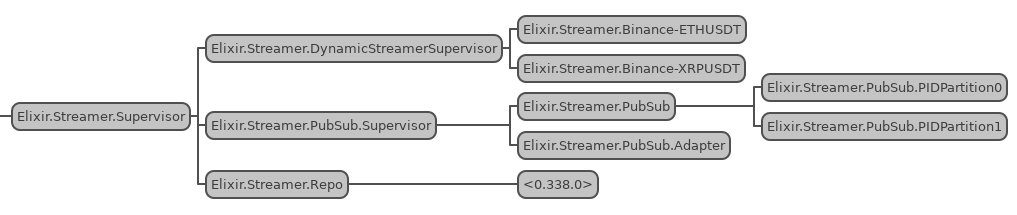
\includegraphics{images/chapter_11_03_first_sup_tree.png}
\caption{DynamicStreamerSupervisor with two \emph{named} streamers}
\end{figure}

\hypertarget{implement-the-stop-functionality}{%
\section{Implement the stop functionality}\label{implement-the-stop-functionality}}

As we can see, we are now registering the \texttt{Streamer.Binance} processes with names that contain their symbols. We will be able to retrieve PIDs of those registered processes just by simply passing the symbol string(ie. ``ETHUSDT'') into \texttt{get\_pid/1}, which will allow us to then request termination of those processes by the \texttt{Streamer.DynamicStreamerSupervisor}.

Let's write a \texttt{stop\_streaming/1} logic inside the \texttt{Streamer.DynamicStreamerSupervisor} module(put it above first private function):

\begin{Shaded}
\begin{Highlighting}[]
  \CommentTok{\# /apps/streamer/lib/streamer/dynamic\_streamer\_supervisor.ex}
  \KeywordTok{def}\NormalTok{ stop\_streaming(symbol) }\KeywordTok{when}\NormalTok{ is\_binary(symbol) }\KeywordTok{do}
    \KeywordTok{case}\NormalTok{ get\_pid(symbol) }\KeywordTok{do}
      \ConstantTok{nil} \OperatorTok{{-}\textgreater{}}
        \ConstantTok{Logger}\OperatorTok{.}\NormalTok{warn(}\StringTok{"Streaming on }\OtherTok{\#\{}\NormalTok{symbol}\OtherTok{\}}\StringTok{ already stopped"}\NormalTok{)}
\NormalTok{        \{}\VariableTok{:ok}\NormalTok{, \_settings\} }\OperatorTok{=}\NormalTok{ update\_streaming\_status(symbol, }\StringTok{"off"}\NormalTok{)}

\NormalTok{      pid }\OperatorTok{{-}\textgreater{}}
        \ConstantTok{Logger}\OperatorTok{.}\NormalTok{info(}\StringTok{"Stopping streaming on }\OtherTok{\#\{}\NormalTok{symbol}\OtherTok{\}}\StringTok{"}\NormalTok{)}

        \VariableTok{:ok} \OperatorTok{=}
          \ConstantTok{DynamicSupervisor}\OperatorTok{.}\NormalTok{terminate\_child(}
            \ConstantTok{Streamer}\OperatorTok{.}\ConstantTok{DynamicStreamerSupervisor}\NormalTok{,}
\NormalTok{            pid}
\NormalTok{          )}

\NormalTok{        \{}\VariableTok{:ok}\NormalTok{, \_settings\} }\OperatorTok{=}\NormalTok{ update\_streaming\_status(symbol, }\StringTok{"off"}\NormalTok{)}
    \KeywordTok{end}
  \KeywordTok{end}
\end{Highlighting}
\end{Shaded}

\texttt{stop\_streaming/1} looks very similar to \texttt{start\_streaming/1}, we are checking is there already a \texttt{Streamer.Binance} process registered for that symbol, and we either ask the \texttt{Streamer.DynamicStreamerSupervisor} to terminate it for us (using the \texttt{DynamicSupervisor.terminate\_child/2} function + update the status) or just update the status to be \texttt{off}.

We need to update the \texttt{Streamer} module to provide the interface to stop streaming on a symbol:

\begin{Shaded}
\begin{Highlighting}[]
\CommentTok{\# /apps/streamer/lib/streamer.ex}
  \OperatorTok{...}
  \KeywordTok{def}\NormalTok{ stop\_streaming(symbol) }\KeywordTok{do}
\NormalTok{    symbol}
    \OperatorTok{|\textgreater{}} \ConstantTok{String}\OperatorTok{.}\NormalTok{upcase()}
    \OperatorTok{|\textgreater{}} \ConstantTok{DynamicStreamerSupervisor}\OperatorTok{.}\NormalTok{stop\_streaming()}
  \KeywordTok{end}
  \OperatorTok{...}
\end{Highlighting}
\end{Shaded}

\hypertarget{implement-the-autostart-streaming-functionality}{%
\section{Implement the autostart streaming functionality}\label{implement-the-autostart-streaming-functionality}}

Currently, whenever we will shutdown the elixir app, settings persist in the database but streamers are not started on the next init.

To fix this, we will add \texttt{autostart\_streaming/0} inside the \texttt{Streamer.DynamicStreamerSupervisor}.

Note: It very important to differentiate between module and process. We will put our autostarting logic inside the \emph{module} but the \texttt{Streamer.DynamicStreamerSupervisor} \emph{process} won't run it.

We will introduce a new \href{https://hexdocs.pm/elixir/master/Task.html}{Task} process that will execute all the autostarting logic.

That will cover the problem of the Supervisor executing too much business logic (as the Task will execute it), but how will we supervise them together?
At init both will start, the \texttt{Streamer.DynamicStreamerSupervisor} first and then Task will ask it to start multiple children and that will work fine. The problem occurs when the \texttt{Streamer.DynamicStreamerSupervisor} would die because of any reason. Currently, it's supervised using the \texttt{one\_for\_one} strategy(and the \texttt{Task} would be as well) which means that it will get started again by the \texttt{Streamer.Application} process but at that moment the ``autostarting'' \texttt{Task} won't be there anymore to start streaming on all enabled symbols.

We can clearly see that whenever the \texttt{Streamer.DynamicStreamerSupervisor} will die it needs to be started again \emph{together} with the ``autostart'' \texttt{Task} and this won't fit our current \texttt{Streamer.Application}'s strategy.

In cases like those, a new level of supervision needs to be introduced that will have a different supervision strategy for those ``coupled'' processes. We will rename the process name of the \texttt{Streamer.Application} (which is currently registered as \texttt{Streamer.Supervisor}) to \texttt{Streamer.Application}. Then we will introduce the new \texttt{Streamer.Supervisor} module and register it under the same name. We will attach both \texttt{Streamer.DynamicStreamerSupervisor} and Task to the \texttt{Streamer.Supervisor} and assign it with the \texttt{rest\_for\_one} strategy which will restart the Task whenever \texttt{Streamer.DynamicStreamerSupervisor} would die:

\begin{figure}
\centering
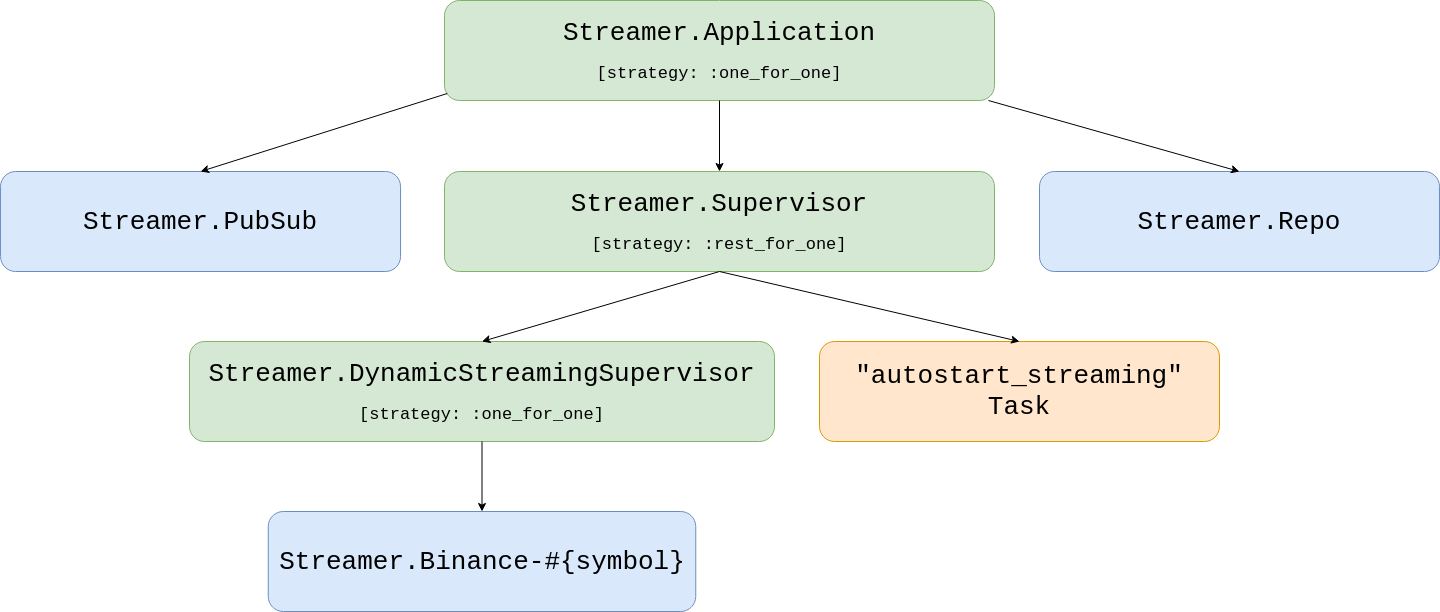
\includegraphics{images/chapter_11_04_new_sup_tree.png}
\caption{Updated supervision tree with additional superviser and renamed Application process}
\end{figure}

Let's start by creating the \texttt{autostart\_streaming/0} functionality inside the \texttt{Streamer.DynamicStreamerSupervisor}:

\begin{Shaded}
\begin{Highlighting}[]
  \CommentTok{\# /apps/streamer/lib/streamer/dynamic\_streamer\_supervisor.ex}

  \CommentTok{\# add below after the \textasciigrave{}init/1\textasciigrave{} function}
  \KeywordTok{def}\NormalTok{ autostart\_streaming() }\KeywordTok{do}
\NormalTok{    fetch\_symbols\_to\_stream()}
    \OperatorTok{|\textgreater{}} \ConstantTok{Enum}\OperatorTok{.}\NormalTok{map(}\OperatorTok{\&}\NormalTok{start\_streaming}\OperatorTok{/}\DecValTok{1}\NormalTok{)}
  \KeywordTok{end}

  \CommentTok{\# and this at the end of the module}
  \KeywordTok{defp}\NormalTok{ fetch\_symbols\_to\_stream() }\KeywordTok{do}
    \ConstantTok{Repo}\OperatorTok{.}\NormalTok{all(}
\NormalTok{      from(s }\KeywordTok{in} \ConstantTok{Settings}\NormalTok{,}
        \VariableTok{where:}\NormalTok{ s}\OperatorTok{.}\NormalTok{status }\OperatorTok{==} \StringTok{"on"}\NormalTok{,}
        \VariableTok{select:}\NormalTok{ s}\OperatorTok{.}\NormalTok{symbol}
\NormalTok{      )}
\NormalTok{    )}
  \KeywordTok{end}
\end{Highlighting}
\end{Shaded}

\texttt{autostart\_streaming/0} function fetches all symbols from the \texttt{settings} table with \texttt{status\ ==\ "on"} then it passes them one by one into the \texttt{start\_streaming/1} function using \texttt{Enum.map/2}.

We can now focus on referring to the above autostarting logic inside the new supervisor that we will create now. Let's start by creating a new file called \texttt{supervisor.ex} inside the \texttt{/apps/streamer/lib/streamer/} directory and fill it with default \href{https://hexdocs.pm/elixir/master/Supervisor.html\#module-module-based-supervisors}{Supervisor} implementation:

\begin{Shaded}
\begin{Highlighting}[]
\CommentTok{\# /apps/streamer/lib/streamer/supervisor.ex}
\KeywordTok{defmodule} \ConstantTok{Streamer}\OperatorTok{.}\ConstantTok{Supervisor} \KeywordTok{do} \CommentTok{\# \textless{}= updated module name}
  \ImportTok{use} \ConstantTok{Supervisor}

  \KeywordTok{def}\NormalTok{ start\_link(init\_arg) }\KeywordTok{do}
    \ConstantTok{Supervisor}\OperatorTok{.}\NormalTok{start\_link(}\ConstantTok{\_\_MODULE\_\_}\NormalTok{, init\_arg, }\VariableTok{name:} \ConstantTok{\_\_MODULE\_\_}\NormalTok{)}
  \KeywordTok{end}

  \KeywordTok{def}\NormalTok{ init(\_init\_arg) }\KeywordTok{do}
\NormalTok{    children }\OperatorTok{=}\NormalTok{ [}

\NormalTok{    ]}

    \ConstantTok{Supervisor}\OperatorTok{.}\NormalTok{init(children, }\VariableTok{strategy:} \VariableTok{:one\_for\_one}\NormalTok{)}
  \KeywordTok{end}
\KeywordTok{end}
\end{Highlighting}
\end{Shaded}

We can now update the strategy to \texttt{rest\_for\_one}:

\begin{Shaded}
\begin{Highlighting}[]
\CommentTok{\# /apps/streamer/lib/streamer/supervisor.ex}
  \KeywordTok{def}\NormalTok{ init(\_init\_arg) }\KeywordTok{do}
    \OperatorTok{...}
    \ConstantTok{Supervisor}\OperatorTok{.}\NormalTok{init(children, }\VariableTok{strategy:} \VariableTok{:rest\_for\_one}\NormalTok{) }\CommentTok{\# \textless{}= strategy updated}
  \KeywordTok{end}
\end{Highlighting}
\end{Shaded}

The last step inside our new supervisor will be to add 2 children: \texttt{Streamer.DynamicStreamerSupervisor} and \texttt{Task} (that will autostart the symbol streamers):

\begin{Shaded}
\begin{Highlighting}[]
\CommentTok{\# /apps/streamer/lib/streamer/supervisor.ex}
  \KeywordTok{def}\NormalTok{ init(\_init\_arg) }\KeywordTok{do}
\NormalTok{    children }\OperatorTok{=}\NormalTok{ [}
\NormalTok{      \{}\ConstantTok{Streamer}\OperatorTok{.}\ConstantTok{DynamicStreamerSupervisor}\NormalTok{, []\},}
\NormalTok{      \{}\ConstantTok{Task}\NormalTok{,}
       \KeywordTok{fn} \OperatorTok{{-}\textgreater{}}
         \ConstantTok{Streamer}\OperatorTok{.}\ConstantTok{DynamicStreamerSupervisor}\OperatorTok{.}\NormalTok{autostart\_streaming()}
       \KeywordTok{end}\NormalTok{\}}
\NormalTok{    ]}
    \OperatorTok{...}
  \KeywordTok{end}
\end{Highlighting}
\end{Shaded}

Final update in this chapter will be to replace the \texttt{Streamer.DynamicStreamerSupervisor} as one of the children inside the \texttt{Streamer.Application} module and update the name that application process registers under:

\begin{Shaded}
\begin{Highlighting}[]
\CommentTok{\# /apps/streamer/lib/streamer/application.ex}
    \OperatorTok{...}
\NormalTok{    children }\OperatorTok{=}\NormalTok{ [}
\NormalTok{      \{}\ConstantTok{Streamer}\OperatorTok{.}\ConstantTok{Repo}\NormalTok{, []\},}
\NormalTok{      \{}
        \ConstantTok{Phoenix}\OperatorTok{.}\ConstantTok{PubSub}\NormalTok{,}
        \VariableTok{name:} \ConstantTok{Streamer}\OperatorTok{.}\ConstantTok{PubSub}\NormalTok{, }\VariableTok{adapter\_name:} \ConstantTok{Phoenix}\OperatorTok{.}\ConstantTok{PubSub}\OperatorTok{.}\ConstantTok{PG2}
\NormalTok{      \},}
\NormalTok{      \{}\ConstantTok{Streamer}\OperatorTok{.}\ConstantTok{Supervisor}\NormalTok{, []\} }\CommentTok{\# \textless{}= updated supervisor}
\NormalTok{    ]}

\NormalTok{    opts }\OperatorTok{=}\NormalTok{ [}\VariableTok{strategy:} \VariableTok{:one\_for\_one}\NormalTok{, }\VariableTok{name:} \ConstantTok{Streamer}\OperatorTok{.}\ConstantTok{Application}\NormalTok{] }\CommentTok{\# \textless{}= updated name}
    \OperatorTok{...}
\end{Highlighting}
\end{Shaded}

\hypertarget{test-the-implementation-3}{%
\section{Test the implementation}\label{test-the-implementation-3}}

Let's start an \texttt{iex} session and call the \texttt{start\_streaming/1} function twice for two different symbols and then exit using double Ctrl+c:

\begin{Shaded}
\begin{Highlighting}[]
\ExtensionTok{$}\NormalTok{ iex }\AttributeTok{{-}S}\NormalTok{ mix}
\ExtensionTok{...}
\ExtensionTok{iex}\ErrorTok{(}\ExtensionTok{1}\KeywordTok{)}\OperatorTok{\textgreater{}}\NormalTok{ Streamer.start\_streaming}\KeywordTok{(}\StringTok{"ethusdt"}\KeywordTok{)}
\ExtensionTok{18:51:39.809}\NormalTok{ [info]  Starting streaming on ETHUSDT}
\ExtensionTok{\{:ok,} \CommentTok{\#PID\textless{}0.370.0\textgreater{}\}}
\ExtensionTok{iex}\ErrorTok{(}\ExtensionTok{2}\KeywordTok{)}\OperatorTok{\textgreater{}}\NormalTok{ Streamer.start\_streaming}\KeywordTok{(}\StringTok{"neousdt"}\KeywordTok{)}
\ExtensionTok{18:51:47.288}\NormalTok{ [info]  Starting streaming on NEOUSDT}
\ExtensionTok{\{:ok,} \CommentTok{\#PID\textless{}0.377.0\textgreater{}\}}
\end{Highlighting}
\end{Shaded}

Now, open a \emph{new} \texttt{iex} session and look at the output:

\begin{Shaded}
\begin{Highlighting}[]
\ExtensionTok{$}\NormalTok{ iex }\AttributeTok{{-}S}\NormalTok{ mix}
\ExtensionTok{...}
\ExtensionTok{iex}\ErrorTok{(}\ExtensionTok{1}\KeywordTok{)}\OperatorTok{\textgreater{}} 
\ExtensionTok{18:53:48.920}\NormalTok{ [info]  Starting streaming on ETHUSDT}
\ExtensionTok{18:53:50.306}\NormalTok{ [info]  Starting streaming on NEOUSDT}
\end{Highlighting}
\end{Shaded}

We can also confirm that streamer processes are there by using \texttt{:observer.start()}:

\begin{figure}
\centering
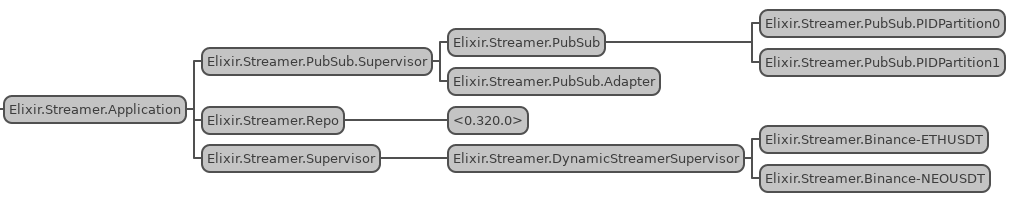
\includegraphics{images/chapter_11_05_finished_tree.png}
\caption{Updated supervision tree with two autostarted streamers and new supervisor}
\end{figure}

Inside the same \texttt{iex} session run the following:

\begin{Shaded}
\begin{Highlighting}[]
\ExtensionTok{iex}\ErrorTok{(}\ExtensionTok{5}\KeywordTok{)}\OperatorTok{\textgreater{}}\NormalTok{ Streamer.stop\_streaming}\KeywordTok{(}\StringTok{"neousdt"}\KeywordTok{)} 
\ExtensionTok{18:57:37.205}\NormalTok{ [info]  Stopping streaming on NEOUSDT}
\ExtensionTok{\{:ok,}
 \ExtensionTok{\%Streamer.Schema.Settings\{}
   \ExtensionTok{...}
 \ErrorTok{\}\}}
\ExtensionTok{iex}\ErrorTok{(}\ExtensionTok{6}\KeywordTok{)}\OperatorTok{\textgreater{}}\NormalTok{ Streamer.stop\_streaming}\KeywordTok{(}\StringTok{"ethusdt"}\KeywordTok{)}
\ExtensionTok{18:57:51.553}\NormalTok{ [info]  Stopping streaming on ETHUSDT}
\ExtensionTok{\{:ok,}
 \ExtensionTok{\%Streamer.Schema.Settings\{}
   \ExtensionTok{...}
 \ErrorTok{\}\}}
\end{Highlighting}
\end{Shaded}

Stop the \texttt{iex} session and start new one - streamers shouldn't be autostarted any more.

{[}Note{]} Please remember to run \texttt{mix\ format} to keep things nice and tidy.

Source code for this chapter can be found at \href{https://github.com/frathon/create-a-cryptocurrency-trading-bot-in-elixir-source-code/tree/chapter_11}{Github}

\hypertarget{start-stop-shutdown-and-autostart-trading}{%
\chapter{Start, stop, shutdown and autostart trading}\label{start-stop-shutdown-and-autostart-trading}}

\hypertarget{objectives-11}{%
\section{Objectives}\label{objectives-11}}

\begin{itemize}
\tightlist
\item
  describe and design the required functionality
\item
  (re-)implement the start trading functionality
\item
  implement the stop trading functionality
\item
  implement the autostart trading functionality
\item
  implement the shutdown trading functionality
\item
  test the implementation
\end{itemize}

\hypertarget{describe-and-design-the-required-functionality-3}{%
\section{Describe and design the required functionality}\label{describe-and-design-the-required-functionality-3}}

In the 10th chapter, we've introduced the Postgres database inside the \texttt{naive} application together with the settings per symbol.

In this chapter, we will progress forward to provide additional trading functionality that will be similar to the functionality implemented in the last chapter for the \texttt{streaming} application:
- stop trading - as the \texttt{Naive.SymbolSupervisor} processes are registered with names that can be easily reverse engineered, we should be able to utilize the \texttt{Process.where\_is/1} function to retrieve the PIDs and instruct the \texttt{Naive.DynamicSymbolSupervisor} to terminate those child processes. Again, we need to put that logic somewhere so we will implement the \texttt{Naive.DynamicSymbolSupervisor} as a full module using the \texttt{DynamicSupervisor} behavior.
- start\_trading - as our \texttt{Naive.DynamicSymbolSupervisor} will now be a module we will be able to remove the \texttt{start\_trading/1} implementation from the \texttt{Naive} module and reimplement it inside the \texttt{Naive.DynamicSymbolSupervisor} module. It will follow the same pattern of checking for PID, starting the \texttt{Naive.SymbolSupervisor} process and flipping the \texttt{status} flag inside the \texttt{settings} table's row for that symbol.
- shutdown trading - sometimes abruptly stopping trading won't be the best solution, it would be better to allow the \texttt{Naive.Trader} processes to finish their ongoing trades. To be able to do that we will need to inform the \texttt{Naive.Leader} process assigned to the symbol that the settings for that symbol have been updated and that should cause the \texttt{Naive.Leader} process to withhold starting new \texttt{Naive.Trader} processes and terminate the whole tree when the last trader will finish.
- autostart trading - this will be a very similar implementation to the one from the last chapter. It will require introducing a new supervisor(we will follow the same naming convention: rename \texttt{Naive.Application}'s registered process name to \texttt{Naive.Application}, create a new supervisor called \texttt{Naive.Supervisor}) and utilize the \texttt{Task} process to execute the autostarting logic.

\begin{figure}
\centering
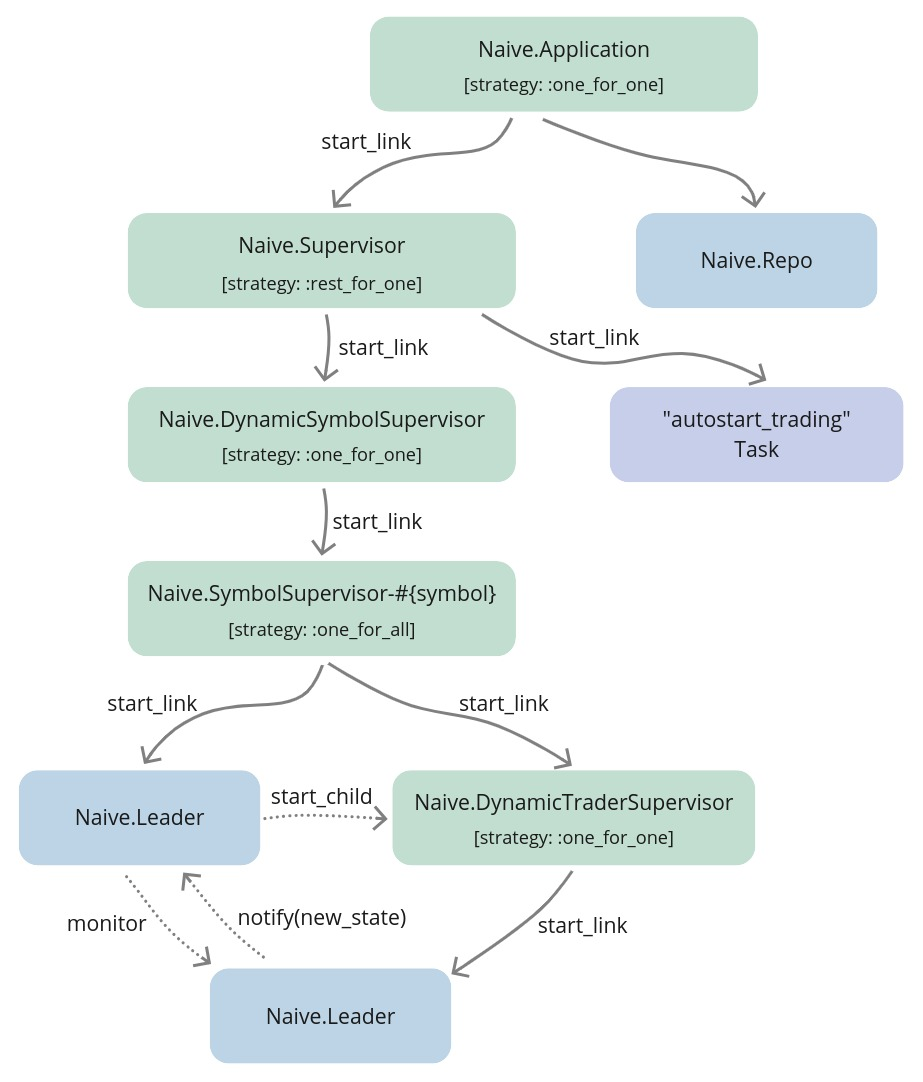
\includegraphics{images/chapter_12_02_sup_diagram.png}
\caption{Final supervision tree after adding the autostarting \texttt{Task} and the Naive.Supervisor}
\end{figure}

\hypertarget{re-implement-the-start-trading-functionality}{%
\section{(Re-)Implement the start trading functionality}\label{re-implement-the-start-trading-functionality}}

To (re-)implement the \texttt{start\_trading/1} functionality we will need to create a new file called \texttt{dynamic\_symbol\_supervisor.ex} inside the \texttt{/apps/naive/lib/naive} directory that will use the \texttt{DynamicSupervisor} behaviour. Previously we have been using default \texttt{DynamicSupervisor} implementation(one of the children of the \texttt{Naive.Application} - to be substituted with the below module):

\begin{Shaded}
\begin{Highlighting}[]
\CommentTok{\# /apps/naive/lib/naive/dynamic\_symbol\_supervisor.ex}
\KeywordTok{defmodule} \ConstantTok{Naive}\OperatorTok{.}\ConstantTok{DynamicSymbolSupervisor} \KeywordTok{do} \CommentTok{\# \textless{}= module updated}
  \ImportTok{use} \ConstantTok{DynamicSupervisor}

  \ImportTok{require} \ConstantTok{Logger} \CommentTok{\# \textless{}= Logger added}

  \ImportTok{import} \ConstantTok{Ecto}\OperatorTok{.}\ConstantTok{Query}\NormalTok{, }\VariableTok{only:}\NormalTok{ [}\VariableTok{from:} \DecValTok{2}\NormalTok{] }\CommentTok{\# \textless{}= added for querying}

  \ImportTok{alias} \ConstantTok{Naive}\OperatorTok{.}\ConstantTok{Repo}             \CommentTok{\# \textless{}= added for querying/updating}
  \ImportTok{alias} \ConstantTok{Naive}\OperatorTok{.}\ConstantTok{Schema}\OperatorTok{.}\ConstantTok{Settings}  \CommentTok{\# \textless{}= added for querying/updating}

  \KeywordTok{def}\NormalTok{ start\_link(init\_arg) }\KeywordTok{do}
    \ConstantTok{DynamicSupervisor}\OperatorTok{.}\NormalTok{start\_link(}\ConstantTok{\_\_MODULE\_\_}\NormalTok{, init\_arg, }\VariableTok{name:} \ConstantTok{\_\_MODULE\_\_}\NormalTok{)}
  \KeywordTok{end}

  \KeywordTok{def}\NormalTok{ init(\_init\_arg) }\KeywordTok{do}
    \ConstantTok{DynamicSupervisor}\OperatorTok{.}\NormalTok{init(}\VariableTok{strategy:} \VariableTok{:one\_for\_one}\NormalTok{)}
  \KeywordTok{end}
\KeywordTok{end}
\end{Highlighting}
\end{Shaded}

The above code is a default implementation from the \href{https://hexdocs.pm/elixir/master/DynamicSupervisor.html\#module-module-based-supervisors}{DynamicSupervisor docs} with some additional imports, require and aliases as we will use them in this chapter.

Our \texttt{start\_trading/1} implementation is almost the same as one for the \texttt{streamer} application from the last chapter:

\begin{Shaded}
\begin{Highlighting}[]
\CommentTok{\# /apps/naive/lib/naive/dynamic\_symbol\_supervisor.ex}
  \OperatorTok{...}
  \KeywordTok{def}\NormalTok{ start\_trading(symbol) }\KeywordTok{when}\NormalTok{ is\_binary(symbol) }\KeywordTok{do}
\NormalTok{    symbol }\OperatorTok{=} \ConstantTok{String}\OperatorTok{.}\NormalTok{upcase(symbol)}
    
    \KeywordTok{case}\NormalTok{ get\_pid(symbol) }\KeywordTok{do}
      \ConstantTok{nil} \OperatorTok{{-}\textgreater{}}
        \ConstantTok{Logger}\OperatorTok{.}\NormalTok{info(}\StringTok{"Starting trading of }\OtherTok{\#\{}\NormalTok{symbol}\OtherTok{\}}\StringTok{"}\NormalTok{)}
\NormalTok{        \{}\VariableTok{:ok}\NormalTok{, \_settings\} }\OperatorTok{=}\NormalTok{ update\_trading\_status(symbol, }\StringTok{"on"}\NormalTok{)}
\NormalTok{        \{}\VariableTok{:ok}\NormalTok{, \_pid\} }\OperatorTok{=}\NormalTok{ start\_symbol\_supervisor(symbol)}

\NormalTok{      pid }\OperatorTok{{-}\textgreater{}}
        \ConstantTok{Logger}\OperatorTok{.}\NormalTok{warn(}\StringTok{"Trading on }\OtherTok{\#\{}\NormalTok{symbol}\OtherTok{\}}\StringTok{ already started"}\NormalTok{)}
\NormalTok{        \{}\VariableTok{:ok}\NormalTok{, \_settings\} }\OperatorTok{=}\NormalTok{ update\_trading\_status(symbol, }\StringTok{"on"}\NormalTok{)}
\NormalTok{        \{}\VariableTok{:ok}\NormalTok{, pid\}}
    \KeywordTok{end}
  \KeywordTok{end}
  \OperatorTok{...}
\end{Highlighting}
\end{Shaded}

together with additional helper functions:

\begin{Shaded}
\begin{Highlighting}[]
\CommentTok{\# /apps/naive/lib/naive/dynamic\_symbol\_supervisor.ex}
  \KeywordTok{defp}\NormalTok{ get\_pid(symbol) }\KeywordTok{do}
    \ConstantTok{Process}\OperatorTok{.}\NormalTok{whereis(:}\StringTok{"Elixir.Naive.SymbolSupervisor{-}}\OtherTok{\#\{}\NormalTok{symbol}\OtherTok{\}}\StringTok{"}\NormalTok{)}
  \KeywordTok{end}

  \KeywordTok{defp}\NormalTok{ update\_trading\_status(symbol, status)}
       \KeywordTok{when}\NormalTok{ is\_binary(symbol) }\KeywordTok{and}\NormalTok{ is\_binary(status) }\KeywordTok{do}
    \ConstantTok{Repo}\OperatorTok{.}\NormalTok{get\_by(}\ConstantTok{Settings}\NormalTok{, }\VariableTok{symbol:}\NormalTok{ symbol)}
    \OperatorTok{|\textgreater{}} \ConstantTok{Ecto}\OperatorTok{.}\ConstantTok{Changeset}\OperatorTok{.}\NormalTok{change(\%\{}\VariableTok{status:}\NormalTok{ status\})}
    \OperatorTok{|\textgreater{}} \ConstantTok{Repo}\OperatorTok{.}\NormalTok{update()}
  \KeywordTok{end}

  \KeywordTok{defp}\NormalTok{ start\_symbol\_supervisor(symbol) }\KeywordTok{do}
    \ConstantTok{DynamicSupervisor}\OperatorTok{.}\NormalTok{start\_child(}
      \ConstantTok{Naive}\OperatorTok{.}\ConstantTok{DynamicSymbolSupervisor}\NormalTok{,}
\NormalTok{      \{}\ConstantTok{Naive}\OperatorTok{.}\ConstantTok{SymbolSupervisor}\NormalTok{, symbol\}}
\NormalTok{    )}
  \KeywordTok{end}
\end{Highlighting}
\end{Shaded}

Both implementation and helper functions are almost the same as the ones inside the \texttt{naive} application. It could be tempting to abstract some of the logic away but remember that we should treat all applications in our umbrella project as standalone services that should not share any code if possible(we broke that rule for the \texttt{TradeEvent} struct from the \texttt{streamer} app but we could easily just make a lib with that struct that would be shared between two applications). I would shy away from sharing any business logic between applications in the umbrella project.

There are two additional places where we need to make updates to get our \texttt{start\_trading/1} to work again:
- we need to update the \texttt{children} list inside the \texttt{Naive.Application}:

\begin{Shaded}
\begin{Highlighting}[]
\CommentTok{\# /apps/naive/lib/naive/application.ex}
    \OperatorTok{...}
\NormalTok{    children }\OperatorTok{=}\NormalTok{ [}
\NormalTok{      \{}\ConstantTok{Naive}\OperatorTok{.}\ConstantTok{Repo}\NormalTok{, []\},}
\NormalTok{      \{}\ConstantTok{Naive}\OperatorTok{.}\ConstantTok{DynamicSymbolSupervisor}\NormalTok{, []\} }\CommentTok{\# \textless{}= replacement of DynamicSupervisor}
\NormalTok{    ]}
\end{Highlighting}
\end{Shaded}

\begin{itemize}
\tightlist
\item
  we need to replace the \texttt{start\_trading/1} implementation inside the \texttt{Naive} module to \texttt{defdelegate} macro(as we don't have any logic to run there):
\end{itemize}

\begin{Shaded}
\begin{Highlighting}[]
\CommentTok{\# /apps/naive/lib/naive.ex}
\OperatorTok{...}
  \ImportTok{alias} \ConstantTok{Naive}\OperatorTok{.}\ConstantTok{DynamicSymbolSupervisor}

  \KeywordTok{defdelegate}\NormalTok{ start\_trading(symbol), }\VariableTok{to:} \ConstantTok{DynamicSymbolSupervisor}
\OperatorTok{...}
\end{Highlighting}
\end{Shaded}

At this moment we are again able to use the \texttt{Naive.start\_trading/1} function to start trading on a symbol (behind the scenes it will use logic from the new \texttt{Naive.DynamicSymbolSupervisor} module).

\hypertarget{implement-the-stop-trading-functionality}{%
\section{Implement the stop trading functionality}\label{implement-the-stop-trading-functionality}}

Stop trading will require a change in two places, first inside the \texttt{Naive.DynamicSymbolSupervisor} where we will place the termination logic:

\begin{Shaded}
\begin{Highlighting}[]
\CommentTok{\# /apps/naive/lib/naive/dynamic\_symbol\_supervisor.ex}
  \OperatorTok{...}
  \KeywordTok{def}\NormalTok{ stop\_trading(symbol) }\KeywordTok{when}\NormalTok{ is\_binary(symbol) }\KeywordTok{do}
\NormalTok{    symbol }\OperatorTok{=} \ConstantTok{String}\OperatorTok{.}\NormalTok{upcase(symbol)}

    \KeywordTok{case}\NormalTok{ get\_pid(symbol) }\KeywordTok{do}
      \ConstantTok{nil} \OperatorTok{{-}\textgreater{}}
        \ConstantTok{Logger}\OperatorTok{.}\NormalTok{warn(}\StringTok{"Trading on }\OtherTok{\#\{}\NormalTok{symbol}\OtherTok{\}}\StringTok{ already stopped"}\NormalTok{)}
\NormalTok{        \{}\VariableTok{:ok}\NormalTok{, \_settings\} }\OperatorTok{=}\NormalTok{ update\_trading\_status(symbol, }\StringTok{"off"}\NormalTok{)}

\NormalTok{      pid }\OperatorTok{{-}\textgreater{}}
        \ConstantTok{Logger}\OperatorTok{.}\NormalTok{info(}\StringTok{"Stopping trading of }\OtherTok{\#\{}\NormalTok{symbol}\OtherTok{\}}\StringTok{"}\NormalTok{)}

        \VariableTok{:ok} \OperatorTok{=}
          \ConstantTok{DynamicSupervisor}\OperatorTok{.}\NormalTok{terminate\_child(}
            \ConstantTok{Naive}\OperatorTok{.}\ConstantTok{DynamicSymbolSupervisor}\NormalTok{,}
\NormalTok{            pid}
\NormalTok{          )}

\NormalTok{        \{}\VariableTok{:ok}\NormalTok{, \_settings\} }\OperatorTok{=}\NormalTok{ update\_trading\_status(symbol, }\StringTok{"off"}\NormalTok{)}
    \KeywordTok{end}
  \KeywordTok{end}
  \OperatorTok{...}
\end{Highlighting}
\end{Shaded}

The second change we need to make is to create a forwarding interface using \texttt{defdelegate} inside the \texttt{Naive} module:

\begin{Shaded}
\begin{Highlighting}[]
\CommentTok{\# /apps/naive/lib/naive.ex}
  \OperatorTok{...}
  \KeywordTok{defdelegate}\NormalTok{ stop\_trading(symbol), }\VariableTok{to:} \ConstantTok{DynamicSymbolSupervisor}
  \OperatorTok{...}
\end{Highlighting}
\end{Shaded}

That pretty much finishes the \texttt{stop\_trading/1} functionality. We are now able to start and stop(what was previously not available) trading on a symbol.

\hypertarget{implement-the-autostart-trading-functionality}{%
\section{Implement the autostart trading functionality}\label{implement-the-autostart-trading-functionality}}

To implement the autostarting we will need to (in a similar fashion as in the last chapter) add a new supervision level that will be dedicated to supervising the \texttt{Naive.DynamicSymbolSupervisor} and the ``autostarting'' \texttt{Task}.

Let's create a new file called \texttt{supervisor.ex} inside the \texttt{/apps/naive/lib/naive} directory and (as in the last chapter) we will add the \texttt{Naive.DynamicSymbolSupervisor} and the \texttt{Task} to its children list. We will also update the supervision strategy to \texttt{:rest\_for\_one}:

\begin{Shaded}
\begin{Highlighting}[]
\CommentTok{\# /apps/naive/lib/naive/supervisor.ex}
\KeywordTok{defmodule} \ConstantTok{Naive}\OperatorTok{.}\ConstantTok{Supervisor} \KeywordTok{do}
  \ImportTok{use} \ConstantTok{Supervisor}

  \KeywordTok{def}\NormalTok{ start\_link(init\_arg) }\KeywordTok{do}
    \ConstantTok{Supervisor}\OperatorTok{.}\NormalTok{start\_link(}\ConstantTok{\_\_MODULE\_\_}\NormalTok{, init\_arg, }\VariableTok{name:} \ConstantTok{\_\_MODULE\_\_}\NormalTok{)}
  \KeywordTok{end}

  \KeywordTok{def}\NormalTok{ init(\_init\_arg) }\KeywordTok{do}
\NormalTok{    children }\OperatorTok{=}\NormalTok{ [}
\NormalTok{      \{}\ConstantTok{Naive}\OperatorTok{.}\ConstantTok{DynamicSymbolSupervisor}\NormalTok{, []\},                 }\CommentTok{\# \textless{}= added}
\NormalTok{      \{}\ConstantTok{Task}\NormalTok{,                                               }\CommentTok{\# \textless{}= added}
       \KeywordTok{fn} \OperatorTok{{-}\textgreater{}}                                               \CommentTok{\# \textless{}= added}
         \ConstantTok{Naive}\OperatorTok{.}\ConstantTok{DynamicSymbolSupervisor}\OperatorTok{.}\NormalTok{autostart\_trading() }\CommentTok{\# \textless{}= added}
       \KeywordTok{end}\NormalTok{\}                                                }\CommentTok{\# \textless{}= added}
\NormalTok{    ]}

    \ConstantTok{Supervisor}\OperatorTok{.}\NormalTok{init(children, }\VariableTok{strategy:} \VariableTok{:rest\_for\_one}\NormalTok{) }\CommentTok{\# \textless{}= strategy updated}
  \KeywordTok{end}
\KeywordTok{end}
\end{Highlighting}
\end{Shaded}

Now we need to swap the \texttt{Naive.DynamicSymbolSupervisor} to \texttt{Naive.Supervisor} in the \texttt{children} list of the \texttt{Naive.Application}, as well as update the registered process' name of the \texttt{Naive.Application}:

\begin{Shaded}
\begin{Highlighting}[]
\CommentTok{\# /apps/naive/lib/naive/application.ex}
  \OperatorTok{...}
  \KeywordTok{def}\NormalTok{ start(\_type, \_args) }\KeywordTok{do}
\NormalTok{    children }\OperatorTok{=}\NormalTok{ [}
\NormalTok{      \{}\ConstantTok{Naive}\OperatorTok{.}\ConstantTok{Repo}\NormalTok{, []\},}
\NormalTok{      \{}\ConstantTok{Naive}\OperatorTok{.}\ConstantTok{Supervisor}\NormalTok{, []\} }\CommentTok{\# \textless{}= replacement for DynamicSymbolSupervisor}
\NormalTok{    ]}

\NormalTok{    opts }\OperatorTok{=}\NormalTok{ [}\VariableTok{strategy:} \VariableTok{:one\_for\_one}\NormalTok{, }\VariableTok{name:} \ConstantTok{Naive}\OperatorTok{.}\ConstantTok{Application}\NormalTok{] }\CommentTok{\# \textless{}= name updated}
\end{Highlighting}
\end{Shaded}

Finally, we need to implement \texttt{autostart\_trading/0} inside the \texttt{Naive.DynamicSymbolSupervisor} module as our new \texttt{Task} refers to it:

\begin{Shaded}
\begin{Highlighting}[]
\CommentTok{\# /apps/naive/lib/naive/dynamic\_symbol\_supervisor.ex}
  \OperatorTok{...}
  \CommentTok{\# add the below function after the \textasciigrave{}init/1\textasciigrave{} function}
  \KeywordTok{def}\NormalTok{ autostart\_trading() }\KeywordTok{do}
\NormalTok{    fetch\_symbols\_to\_trade()}
    \OperatorTok{|\textgreater{}} \ConstantTok{Enum}\OperatorTok{.}\NormalTok{map(}\OperatorTok{\&}\NormalTok{start\_trading}\OperatorTok{/}\DecValTok{1}\NormalTok{)}
  \KeywordTok{end}
 
  \OperatorTok{...}

  \CommentTok{\# and this helper at the end of the module}
  \KeywordTok{defp}\NormalTok{ fetch\_symbols\_to\_trade() }\KeywordTok{do}
    \ConstantTok{Repo}\OperatorTok{.}\NormalTok{all(}
\NormalTok{      from(s }\KeywordTok{in} \ConstantTok{Settings}\NormalTok{,}
        \VariableTok{where:}\NormalTok{ s}\OperatorTok{.}\NormalTok{status }\OperatorTok{==} \StringTok{"on"}\NormalTok{,}
        \VariableTok{select:}\NormalTok{ s}\OperatorTok{.}\NormalTok{symbol}
\NormalTok{      )}
\NormalTok{    )}
  \KeywordTok{end}
  \OperatorTok{...}
\end{Highlighting}
\end{Shaded}

Those are the same (excluding updated function names) as inside the \texttt{streamer} application. We are fetching enabled symbols and starting new \texttt{Naive.SymbolSupervisor} processes for each one.

At this moment we can already see our implementation in action:

\begin{figure}
\centering
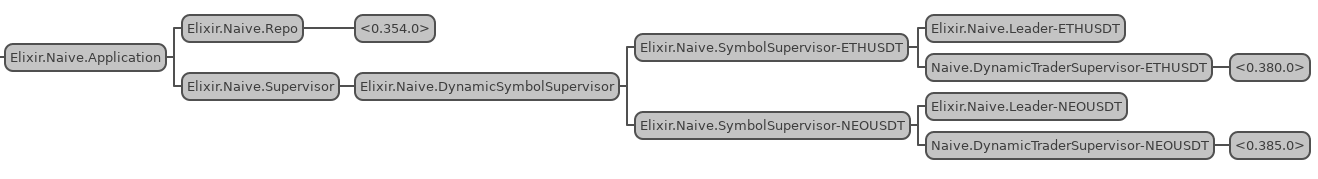
\includegraphics{images/chapter_12_01_autostarting_sup_tree.png}
\caption{Trading on two symbols autostarted, new Naive.Supervisor and renamed Naive.Application}
\end{figure}

At this moment we are able to test the current implementation inside the \texttt{iex}:

\begin{Shaded}
\begin{Highlighting}[]
\ExtensionTok{$}\NormalTok{ iex }\AttributeTok{{-}S}\NormalTok{ mix}
\ExtensionTok{...}
\ExtensionTok{iex}\ErrorTok{(}\ExtensionTok{1}\KeywordTok{)}\OperatorTok{\textgreater{}}\NormalTok{ Naive.start\_trading}\KeywordTok{(}\StringTok{"ethusdt"}\KeywordTok{)}
\ExtensionTok{21:35:30.207}\NormalTok{ [info]  Starting trading of ETHUSDT}
\ExtensionTok{21:35:30.261}\NormalTok{ [info]  Starting new supervision tree to trade on ETHUSDT}
\ExtensionTok{\{:ok,} \CommentTok{\#PID\textless{}0.372.0\textgreater{}\}}
\ExtensionTok{21:35:33.344}\NormalTok{ [info]  Initializing new trader}\ErrorTok{(}\ExtensionTok{1612647333342}\KeywordTok{)} \ControlFlowTok{for}\NormalTok{ ETHUSDT}
\ExtensionTok{iex}\ErrorTok{(}\ExtensionTok{3}\KeywordTok{)}\OperatorTok{\textgreater{}}\NormalTok{ Naive.start\_trading}\KeywordTok{(}\StringTok{"neousdt"}\KeywordTok{)}    
\ExtensionTok{21:35:54.128}\NormalTok{ [info]  Starting trading of NEOUSDT}
\ExtensionTok{21:35:54.169}\NormalTok{ [info]  Starting new supervision tree to trade on NEOUSDT}
\ExtensionTok{\{:ok,} \CommentTok{\#PID\textless{}0.383.0\textgreater{}\}}
\ExtensionTok{21:35:56.007}\NormalTok{ [info]  Initializing new trader}\ErrorTok{(}\ExtensionTok{1612647356007}\KeywordTok{)} \ControlFlowTok{for}\NormalTok{ NEOUSDT}
\ExtensionTok{21:38:07.699}\NormalTok{ [info]  Stopping trading of NEOUSDT}
\ExtensionTok{\{:ok,}
 \ExtensionTok{\%Naive.Schema.Settings\{}
     \ExtensionTok{...}
 \ErrorTok{\}\}}
\end{Highlighting}
\end{Shaded}

We can now exit the \texttt{iex} and start a new one:

\begin{Shaded}
\begin{Highlighting}[]
\ExtensionTok{$}\NormalTok{ iex }\AttributeTok{{-}S}\NormalTok{ mix}
\ExtensionTok{...}
\ExtensionTok{21:39:16.894}\NormalTok{ [info]  Starting trading of ETHUSDT}
\ExtensionTok{21:39:16.938}\NormalTok{ [info]  Starting new supervision tree to trade on ETHUSDT}
\ExtensionTok{21:39:18.786}\NormalTok{ [info]  Initializing new trader}\ErrorTok{(}\ExtensionTok{1612647558784}\KeywordTok{)} \ControlFlowTok{for}\NormalTok{ ETHUSDT}
\ExtensionTok{iex}\ErrorTok{(}\ExtensionTok{1}\KeywordTok{)}\OperatorTok{\textgreater{}}
\end{Highlighting}
\end{Shaded}

The above logs confirm that the \texttt{naive} application autostarts the previously enabled symbols(using the \texttt{start\_trading/1} function) as well as \texttt{stop\_trading/1} updates the status inside the database (so the symbol isn't autostarted at the next initialization).

\hypertarget{implement-the-shutdown-trading-functionality}{%
\section{Implement the shutdown trading functionality}\label{implement-the-shutdown-trading-functionality}}

Last but not least, we will move on to the \texttt{shutdown\_trading/1} functionality. Let's start with the simplest part which is delegating the function call to the \texttt{Naive.DynamicSymbolSupervisor} module from the \texttt{Naive} module(interface):

\begin{Shaded}
\begin{Highlighting}[]
  \CommentTok{\# /apps/naive/lib/naive.ex}
  \OperatorTok{...}
  \KeywordTok{defdelegate}\NormalTok{ shutdown\_trading(symbol), }\VariableTok{to:} \ConstantTok{DynamicSymbolSupervisor}
  \OperatorTok{...}
\end{Highlighting}
\end{Shaded}

Next, we will create a \texttt{shutdown\_trading/1} function inside the \texttt{Naive.DynamicSymbolSupervisor} module where we will check is there any trading going on for that symbol(the same as for start/stop), and in case of trading happening we will inform the \texttt{Naive.Leader} process handling that symbol that settings have been updated:

\begin{Shaded}
\begin{Highlighting}[]
\CommentTok{\# /apps/naive/lib/naive/dynamic\_symbol\_supervisor.ex}
  \OperatorTok{...}
  \KeywordTok{def}\NormalTok{ shutdown\_trading(symbol) }\KeywordTok{when}\NormalTok{ is\_binary(symbol) }\KeywordTok{do}
\NormalTok{    symbol }\OperatorTok{=} \ConstantTok{String}\OperatorTok{.}\NormalTok{upcase(symbol)}

    \KeywordTok{case}\NormalTok{ get\_pid(symbol) }\KeywordTok{do}
      \ConstantTok{nil} \OperatorTok{{-}\textgreater{}}
        \ConstantTok{Logger}\OperatorTok{.}\NormalTok{warn(}\StringTok{"Trading on }\OtherTok{\#\{}\NormalTok{symbol}\OtherTok{\}}\StringTok{ already stopped"}\NormalTok{)}
\NormalTok{        \{}\VariableTok{:ok}\NormalTok{, \_settings\} }\OperatorTok{=}\NormalTok{ update\_trading\_status(symbol, }\StringTok{"off"}\NormalTok{)}

\NormalTok{      \_pid }\OperatorTok{{-}\textgreater{}}
        \ConstantTok{Logger}\OperatorTok{.}\NormalTok{info(}\StringTok{"Shutdown of trading on }\OtherTok{\#\{}\NormalTok{symbol}\OtherTok{\}}\StringTok{ initialized"}\NormalTok{)}
\NormalTok{        \{}\VariableTok{:ok}\NormalTok{, settings\} }\OperatorTok{=}\NormalTok{ update\_trading\_status(symbol, }\StringTok{"shutdown"}\NormalTok{)}
        \ConstantTok{Naive}\OperatorTok{.}\ConstantTok{Leader}\OperatorTok{.}\NormalTok{notify(}\VariableTok{:settings\_updated}\NormalTok{, settings)}
\NormalTok{        \{}\VariableTok{:ok}\NormalTok{, settings\}}
    \KeywordTok{end}
  \KeywordTok{end}
  \OperatorTok{...}
\end{Highlighting}
\end{Shaded}

The crucial part of the implementation above is the \texttt{notify(:settings\_updated,\ settings)} where we inform the \texttt{Naive.Leader} process that it needs to update trading settings.

Currently, the \texttt{Naive.Leader} module does \emph{not} support updating the settings after startup - let's add a new interface function together with a callback function that will handle settings updating:

\begin{Shaded}
\begin{Highlighting}[]
\CommentTok{\# /apps/naive/lib/naive/leader.ex}
  \OperatorTok{...}
  \CommentTok{\# add the below function as the last clause of the \textasciigrave{}notify\textasciigrave{} function}
  \KeywordTok{def}\NormalTok{ notify(}\VariableTok{:settings\_updated}\NormalTok{, settings) }\KeywordTok{do}
    \ConstantTok{GenServer}\OperatorTok{.}\NormalTok{call(}
\NormalTok{      :}\StringTok{"}\OtherTok{\#\{}\ConstantTok{\_\_MODULE\_\_}\OtherTok{\}}\StringTok{{-}}\OtherTok{\#\{}\NormalTok{settings}\OperatorTok{.}\NormalTok{symbol}\OtherTok{\}}\StringTok{"}\NormalTok{,}
\NormalTok{      \{}\VariableTok{:update\_settings}\NormalTok{, settings\}}
\NormalTok{    )}
  \KeywordTok{end}

  \CommentTok{\# add the below handler function as the last clause of \textasciigrave{}handle\_call\textasciigrave{} function}
  \KeywordTok{def}\NormalTok{ handle\_call(}
\NormalTok{        \{}\VariableTok{:update\_settings}\NormalTok{, new\_settings\},}
\NormalTok{        \_,}
\NormalTok{        state}
\NormalTok{      ) }\KeywordTok{do}
\NormalTok{    \{}\VariableTok{:reply}\NormalTok{, }\VariableTok{:ok}\NormalTok{, \%\{state }\OperatorTok{|} \VariableTok{settings:}\NormalTok{ new\_settings\}\}}
  \KeywordTok{end}
\end{Highlighting}
\end{Shaded}

Ok, we have a way to update the settings of the \texttt{Naive.Leader} process ``on the go'' but what effects should the \texttt{shutdown} state have on the \texttt{Naive.Leader}'s actions?

There are two places that require modification:
- whenever the \texttt{Naive.Trader} process will finish the trade cycle, \texttt{Naive.Leader} process should \emph{not} start a new one, as well as check, was that the last trader process and if that was the case it needs to call the \texttt{Naive.stop\_trading/1} function with its symbol to terminate whole supervision tree for that symbol
- whenever the \texttt{Naive.Leader} process will receive a \texttt{rebuy} notification, it should just ignore it when the symbol is in the \texttt{shutdown} state.

Let's look at the updated implementation of the ``end of trade'' handler:

\begin{Shaded}
\begin{Highlighting}[]
\CommentTok{\# /apps/naive/lib/naive/leader.ex}
  \OperatorTok{...}
  \KeywordTok{def}\NormalTok{ handle\_info(}
\NormalTok{        \{}\VariableTok{:DOWN}\NormalTok{, \_ref, }\VariableTok{:process}\NormalTok{, trader\_pid, }\VariableTok{:normal}\NormalTok{\},}
\NormalTok{        \%\{}\VariableTok{traders:}\NormalTok{ traders, }\VariableTok{symbol:}\NormalTok{ symbol, }\VariableTok{settings:}\NormalTok{ settings\} }\OperatorTok{=}\NormalTok{ state}
\NormalTok{      ) }\KeywordTok{do}
    \ConstantTok{Logger}\OperatorTok{.}\NormalTok{info(}\StringTok{"}\OtherTok{\#\{}\NormalTok{symbol}\OtherTok{\}}\StringTok{ trader finished trade {-} restarting"}\NormalTok{)}

    \KeywordTok{case} \ConstantTok{Enum}\OperatorTok{.}\NormalTok{find\_index(traders, }\OperatorTok{\&}\NormalTok{(}\OperatorTok{\&}\DecValTok{1}\OperatorTok{.}\NormalTok{pid }\OperatorTok{==}\NormalTok{ trader\_pid)) }\KeywordTok{do}
      \ConstantTok{nil} \OperatorTok{{-}\textgreater{}}
        \ConstantTok{Logger}\OperatorTok{.}\NormalTok{warn(}
          \StringTok{"Tried to restart finished }\OtherTok{\#\{}\NormalTok{symbol}\OtherTok{\}}\StringTok{ "} \OperatorTok{\textless{}\textgreater{}}
            \StringTok{"trader that leader is not aware of"}
\NormalTok{        )}

        \ControlFlowTok{if}\NormalTok{ settings}\OperatorTok{.}\NormalTok{status }\OperatorTok{==} \StringTok{"shutdown"} \KeywordTok{and}\NormalTok{ traders }\OperatorTok{==}\NormalTok{ [] }\KeywordTok{do} \CommentTok{\# \textless{}= additional check}
          \ConstantTok{Naive}\OperatorTok{.}\NormalTok{stop\_trading(state}\OperatorTok{.}\NormalTok{symbol)}
        \KeywordTok{end}

\NormalTok{        \{}\VariableTok{:noreply}\NormalTok{, state\}}

\NormalTok{      index }\OperatorTok{{-}\textgreater{}}
\NormalTok{        new\_traders }\OperatorTok{=}
          \ControlFlowTok{if}\NormalTok{ settings}\OperatorTok{.}\NormalTok{status }\OperatorTok{==} \StringTok{"shutdown"} \KeywordTok{do} \CommentTok{\# \textless{}= refactored code}
            \ConstantTok{Logger}\OperatorTok{.}\NormalTok{warn(}
              \StringTok{"The leader won\textquotesingle{}t start a new trader on }\OtherTok{\#\{}\NormalTok{symbol}\OtherTok{\}}\StringTok{ "} \OperatorTok{\textless{}\textgreater{}}
                \StringTok{"as symbol is in the \textquotesingle{}shutdown\textquotesingle{} state"}
\NormalTok{            )}
            
            \ControlFlowTok{if}\NormalTok{ length(traders) }\OperatorTok{==} \DecValTok{1} \KeywordTok{do}
              \ConstantTok{Naive}\OperatorTok{.}\NormalTok{stop\_trading(state}\OperatorTok{.}\NormalTok{symbol)}
            \KeywordTok{end}
            
            \ConstantTok{List}\OperatorTok{.}\NormalTok{delete\_at(traders, index)}
          \ControlFlowTok{else}
\NormalTok{            new\_trader\_data }\OperatorTok{=}\NormalTok{ start\_new\_trader(fresh\_trader\_state(settings))}
            \ConstantTok{List}\OperatorTok{.}\NormalTok{replace\_at(traders, index, new\_trader\_data)}
          \KeywordTok{end}

\NormalTok{        \{}\VariableTok{:noreply}\NormalTok{, \%\{state }\OperatorTok{|} \VariableTok{traders:}\NormalTok{ new\_traders\}\}}
    \KeywordTok{end}
  \KeywordTok{end}
  \OperatorTok{...}
\end{Highlighting}
\end{Shaded}

As visible in the above code, whenever the \texttt{Naive.Trader} process will finish the trade cycle, the \texttt{Naive.Leader} process will check can it find a record of that trader in its state (no changes here). We will modify the callback so the leader process will check the \texttt{settings.status}. In the \texttt{shutdown} status it checks wheater it was the last trader in the \texttt{traders} list, to terminate the whole tree at that time(using the \texttt{Naive.stop\_trading/1} function).

The second callback that we need to modify is the \texttt{rebuy} triggered:

\begin{Shaded}
\begin{Highlighting}[]
\CommentTok{\# /apps/naive/lib/naive/leader.ex}
  \OperatorTok{...}
  \KeywordTok{def}\NormalTok{ handle\_call(}
\NormalTok{        \{}\VariableTok{:rebuy\_triggered}\NormalTok{, new\_trader\_state\},}
\NormalTok{        \{trader\_pid, \_\},}
\NormalTok{        \%\{}\VariableTok{traders:}\NormalTok{ traders, }\VariableTok{symbol:}\NormalTok{ symbol, }\VariableTok{settings:}\NormalTok{ settings\} }\OperatorTok{=}\NormalTok{ state}
\NormalTok{      ) }\KeywordTok{do}
    \KeywordTok{case} \ConstantTok{Enum}\OperatorTok{.}\NormalTok{find\_index(traders, }\OperatorTok{\&}\NormalTok{(}\OperatorTok{\&}\DecValTok{1}\OperatorTok{.}\NormalTok{pid }\OperatorTok{==}\NormalTok{ trader\_pid)) }\KeywordTok{do}
      \ConstantTok{nil} \OperatorTok{{-}\textgreater{}}
        \ConstantTok{Logger}\OperatorTok{.}\NormalTok{warn(}\StringTok{"Rebuy triggered by trader that leader is not aware of"}\NormalTok{)}
\NormalTok{        \{}\VariableTok{:reply}\NormalTok{, }\VariableTok{:ok}\NormalTok{, state\}}

\NormalTok{      index }\OperatorTok{{-}\textgreater{}}
\NormalTok{        old\_trader\_data }\OperatorTok{=} \ConstantTok{Enum}\OperatorTok{.}\NormalTok{at(traders, index)}
\NormalTok{        new\_trader\_data }\OperatorTok{=}\NormalTok{ \%\{old\_trader\_data }\OperatorTok{|} \VariableTok{:state} \OperatorTok{=\textgreater{}}\NormalTok{ new\_trader\_state\}}
\NormalTok{        updated\_traders }\OperatorTok{=} \ConstantTok{List}\OperatorTok{.}\NormalTok{replace\_at(traders, index, new\_trader\_data)}

\NormalTok{        updated\_traders }\OperatorTok{=}
          \ControlFlowTok{if}\NormalTok{ settings}\OperatorTok{.}\NormalTok{chunks }\OperatorTok{==}\NormalTok{ length(traders) }\KeywordTok{do}
            \ConstantTok{Logger}\OperatorTok{.}\NormalTok{info(}\StringTok{"All traders already started for }\OtherTok{\#\{}\NormalTok{symbol}\OtherTok{\}}\StringTok{"}\NormalTok{)}
\NormalTok{            updated\_traders}
          \ControlFlowTok{else}
            \ControlFlowTok{if}\NormalTok{ settings}\OperatorTok{.}\NormalTok{status }\OperatorTok{==} \StringTok{"shutdown"} \KeywordTok{do}
              \ConstantTok{Logger}\OperatorTok{.}\NormalTok{warn(}
                \StringTok{"The leader won\textquotesingle{}t start a new trader on }\OtherTok{\#\{}\NormalTok{symbol}\OtherTok{\}}\StringTok{ "} \OperatorTok{\textless{}\textgreater{}}
                  \StringTok{"as symbol is in the \textquotesingle{}shutdown\textquotesingle{} state"}
\NormalTok{              )}

\NormalTok{              updated\_traders}
            \ControlFlowTok{else}
              \ConstantTok{Logger}\OperatorTok{.}\NormalTok{info(}\StringTok{"Starting new trader for }\OtherTok{\#\{}\NormalTok{symbol}\OtherTok{\}}\StringTok{"}\NormalTok{)}
\NormalTok{              [start\_new\_trader(fresh\_trader\_state(settings)) }\OperatorTok{|}\NormalTok{ updated\_traders]}
            \KeywordTok{end}
          \KeywordTok{end}

\NormalTok{        \{}\VariableTok{:reply}\NormalTok{, }\VariableTok{:ok}\NormalTok{, \%\{state }\OperatorTok{|} \VariableTok{:traders} \OperatorTok{=\textgreater{}}\NormalTok{ updated\_traders\}\}}
    \KeywordTok{end}
  \KeywordTok{end}
  \OperatorTok{...}
\end{Highlighting}
\end{Shaded}

In the above \texttt{rebuy\_triggered} handler function we added branching on the \texttt{settings.status} and we simply ignore the rebuy notification when the symbol is in the \texttt{shutdown} status.

The final change will be to create a new migration that will update the \texttt{TradingStatusEnum} to have \texttt{shutdown} option:

\begin{Shaded}
\begin{Highlighting}[]
\ExtensionTok{$}\NormalTok{ cd apps/naive }
\ExtensionTok{$}\NormalTok{ mix ecto.gen.migration update\_trading\_status}
\ExtensionTok{*}\NormalTok{ creating priv/repo/migrations/20210205232303\_update\_trading\_status.exs}
\end{Highlighting}
\end{Shaded}

Inside the generated migration file we need to excute a raw SQL command:

\begin{Shaded}
\begin{Highlighting}[]
\CommentTok{\# /apps/naive/priv/repo/migrations/20210205232303\_update\_trading\_status.exs}
\KeywordTok{defmodule} \ConstantTok{Naive}\OperatorTok{.}\ConstantTok{Repo}\OperatorTok{.}\ConstantTok{Migrations}\OperatorTok{.}\ConstantTok{UpdateTradingStatus} \KeywordTok{do}
  \ImportTok{use} \ConstantTok{Ecto}\OperatorTok{.}\ConstantTok{Migration}

  \OtherTok{@disable\_ddl\_transaction} \ConstantTok{true}

  \KeywordTok{def}\NormalTok{ change }\KeywordTok{do}
    \ConstantTok{Ecto}\OperatorTok{.}\ConstantTok{Migration}\OperatorTok{.}\NormalTok{execute }\StringTok{"ALTER TYPE trading\_status ADD VALUE IF NOT EXISTS \textquotesingle{}shutdown\textquotesingle{}"}
  \KeywordTok{end}
\KeywordTok{end}
\end{Highlighting}
\end{Shaded}

We need to apply the same change to the \texttt{Naive.Schema.TradingStatusEnum}:

\begin{Shaded}
\begin{Highlighting}[]
\CommentTok{\# /apps/naive/lib/naive/schema/trading\_status\_enum.ex}
\ImportTok{import} \ConstantTok{EctoEnum}

\NormalTok{defenum(}\ConstantTok{Naive}\OperatorTok{.}\ConstantTok{Schema}\OperatorTok{.}\ConstantTok{TradingStatusEnum}\NormalTok{, }\VariableTok{:trading\_status}\NormalTok{, [}\VariableTok{:on}\NormalTok{, }\VariableTok{:off}\NormalTok{, }\VariableTok{:shutdown}\NormalTok{])}
\end{Highlighting}
\end{Shaded}

Don't forget to run \texttt{mix\ ecto.migrate} to run the new migration.

We can now test the \texttt{shutdown\_trading/1} functionality inside the \texttt{iex}:

\begin{Shaded}
\begin{Highlighting}[]
\ExtensionTok{$}\NormalTok{ iex }\AttributeTok{{-}S}\NormalTok{ mix}
\ExtensionTok{...}
\ExtensionTok{iex}\ErrorTok{(}\ExtensionTok{1}\KeywordTok{)}\OperatorTok{\textgreater{}}\NormalTok{ Streamer.start\_streaming}\KeywordTok{(}\StringTok{"ethusdt"}\KeywordTok{)}
\ExtensionTok{21:46:26.651}\NormalTok{ [info]  Starting streaming on ETHUSDT}
\ExtensionTok{\{:ok,} \CommentTok{\#PID\textless{}0.372.0\textgreater{}\}}
\ExtensionTok{iex}\ErrorTok{(}\ExtensionTok{2}\KeywordTok{)}\OperatorTok{\textgreater{}}\NormalTok{ Naive.start\_trading}\KeywordTok{(}\StringTok{"ethusdt"}\KeywordTok{)}     
\ExtensionTok{21:46:42.830}\NormalTok{ [info]  Starting trading of ETHUSDT}
\ExtensionTok{21:46:42.867}\NormalTok{ [info]  Starting new supervision tree to trade on ETHUSDT}
\ExtensionTok{\{:ok,} \CommentTok{\#PID\textless{}0.379.0\textgreater{}\}}
\ExtensionTok{21:46:44.816}\NormalTok{ [info]  Initializing new trader}\ErrorTok{(}\ExtensionTok{1612648004814}\KeywordTok{)} \ControlFlowTok{for}\NormalTok{ ETHUSDT}
\ExtensionTok{...}
\ExtensionTok{21:47:52.448}\NormalTok{ [info]  Rebuy triggered for ETHUSDT by the trader}\ErrorTok{(}\ExtensionTok{1612648004814}\KeywordTok{)}
\ExtensionTok{...}
\ExtensionTok{21:49:58.900}\NormalTok{ [info]  Rebuy triggered for ETHUSDT by the trader}\ErrorTok{(}\ExtensionTok{1612648089409}\KeywordTok{)}
\ExtensionTok{...}
\ExtensionTok{21:50:58.927}\NormalTok{ [info]  Rebuy triggered for ETHUSDT by the trader}\ErrorTok{(}\ExtensionTok{1612648198900}\KeywordTok{)}
\ExtensionTok{...}
\ExtensionTok{21:53:27.202}\NormalTok{ [info]  Rebuy triggered for ETHUSDT by the trader}\ErrorTok{(}\ExtensionTok{1612648326215}\KeywordTok{)}
\ExtensionTok{21:53:27.250}\NormalTok{ [info]  Rebuy triggered for ETHUSDT by the trader}\ErrorTok{(}\ExtensionTok{1612648325512}\KeywordTok{)}
\ExtensionTok{21:53:27.250}\NormalTok{ [info]  All traders already started for ETHUSDT}

\CommentTok{\# at this moment we have 5 \textasciigrave{}Naive.Trader\textasciigrave{} processes trading in parallel}

\ExtensionTok{iex}\ErrorTok{(}\ExtensionTok{4}\KeywordTok{)}\OperatorTok{\textgreater{}}\NormalTok{ Naive.shutdown\_trading}\KeywordTok{(}\StringTok{"ethusdt"}\KeywordTok{)}
\ExtensionTok{21:55:01.556}\NormalTok{ [info]  Shutdown of trading on ETHUSDT initialized}
\ExtensionTok{\{:ok,}
 \ExtensionTok{\%Naive.Schema.Settings\{}
     \ExtensionTok{...}
 \ErrorTok{\}\}}
\ExtensionTok{...}
\ExtensionTok{22:06:58.855}\NormalTok{ [info]  Trader}\ErrorTok{(}\ExtensionTok{1612648407202}\KeywordTok{)} \ExtensionTok{finished}\NormalTok{ trade cycle for ETHUSDT}
\ExtensionTok{22:06:58.855}\NormalTok{ [info]  ETHUSDT trader finished trade }\AttributeTok{{-}}\NormalTok{ restarting}
\ExtensionTok{22:06:58.855}\NormalTok{ [warn]  The leader won}\StringTok{\textquotesingle{}t start a new trader on ETHUSDTas symbol is in shutdown state}
\StringTok{22:07:50.768 [info]  Trader(1612648325512) finished trade cycle for ETHUSDT}
\StringTok{22:07:50.768 [info]  ETHUSDT trader finished trade {-} restarting}
\StringTok{22:07:50.768 [warn]  The leader won\textquotesingle{}}\NormalTok{t start a new trader on ETHUSDTas symbol is in shutdown state}
\ExtensionTok{22:07:50.857}\NormalTok{ [info]  Trader}\ErrorTok{(}\ExtensionTok{1612648326215}\KeywordTok{)} \ExtensionTok{finished}\NormalTok{ trade cycle for ETHUSDT}
\ExtensionTok{22:07:50.857}\NormalTok{ [info]  ETHUSDT trader finished trade }\AttributeTok{{-}}\NormalTok{ restarting}
\ExtensionTok{22:07:50.857}\NormalTok{ [warn]  The leader won}\StringTok{\textquotesingle{}t start a new trader on ETHUSDTas symbol is in shutdown state}
\StringTok{22:07:51.079 [info]  Trader(1612648089409) finished trade cycle for ETHUSDT}
\StringTok{22:07:51.079 [info]  ETHUSDT trader finished trade {-} restarting}
\StringTok{22:07:51.079 [warn]  The leader won\textquotesingle{}}\NormalTok{t start a new trader on ETHUSDTas symbol is in shutdown state}
\ExtensionTok{22:08:05.401}\NormalTok{ [info]  Trader}\ErrorTok{(}\ExtensionTok{1612648004814}\KeywordTok{)} \ExtensionTok{finished}\NormalTok{ trade cycle for ETHUSDT}
\ExtensionTok{22:08:05.401}\NormalTok{ [info]  ETHUSDT trader finished trade }\AttributeTok{{-}}\NormalTok{ restarting}
\ExtensionTok{22:08:05.401}\NormalTok{ [warn]  The leader won}\StringTok{\textquotesingle{}t start a new trader on ETHUSDTas symbol is in shutdown state}
\StringTok{22:08:05.401 [info]  Stopping trading of ETHUSDT}
\end{Highlighting}
\end{Shaded}

As we can see from the logs above, our \texttt{naive} strategy grown from 1 to 5 \texttt{Naive.Trader} processes running in parallel, then we called the \texttt{shutdown\_trading/1} function. In the \texttt{shutdown} status, the \texttt{Naive.Leader} process ignored \texttt{rebuy} notifications and wasn't starting any new \texttt{Naive.Trader} processes as the old ones were finishing. At the moment when the last \texttt{Naive.Trader} process finished the trade cycle, the \texttt{Naive.Leader} called \texttt{stop\_trading/1} on ``it's'' symbol, terminating the whole supervision tree for that symbol.

{[}Note{]} Please remember to run \texttt{mix\ format} to keep things nice and tidy.

Source code for this chapter can be found at \href{https://github.com/frathon/create-a-cryptocurrency-trading-bot-in-elixir-source-code/tree/chapter_12}{Github}

\hypertarget{abstract-duplicated-supervision-code}{%
\chapter{Abstract duplicated supervision code}\label{abstract-duplicated-supervision-code}}

\hypertarget{objectives-12}{%
\section{Objectives}\label{objectives-12}}

\begin{itemize}
\tightlist
\item
  overview of requirements
\item
  pseudo generalize \texttt{Core.ServiceSupervisor} module
\item
  utilize pseudo generalized code inside the \texttt{Naive.DynamicSymbolSupervisor}
\item
  implement a truly generic \texttt{Core.ServiceSupervisor}
\item
  use the \texttt{Core.ServiceSupervisor} module inside the \texttt{streamer} application
\end{itemize}

\hypertarget{overview-of-requirements}{%
\section{Overview of requirements}\label{overview-of-requirements}}

In the last few chapters, we went through adding and modifying the dynamic supervision tree around the \texttt{naive} and \texttt{streamer} applications' workers. Initially, we just copied the implementation from the \texttt{streamer} application to the \texttt{naive} application (with a few minor tweaks like log messages). That wasn't the most sophisticated solution and we will address this copy-paste pattern in this chapter.

We will write an ``extension'' of the \texttt{DynamicSupervisor} that allows to start, stop and autostart workers. Just to keep things simple we will create a new application inside our umbrella project where we will place the logic. This will save us from creating a new repo for time being.

Our new \texttt{Core.ServiceSupervisor} module will hold all the logic responsible for starting, stopping, and autostarting worker processes. To limit the boilerplate inside the implementation modules (like \texttt{Naive.DynamicSymbolSupervisor} or \texttt{Streamer.DynamicStreamerSupervisor}) we will utilize the \texttt{use} macro that will dynamically generate low-level wiring for us.

\hypertarget{pseudo-generalize-core.servicesupervisor-module}{%
\section{Pseudo generalize Core.ServiceSupervisor module}\label{pseudo-generalize-core.servicesupervisor-module}}

Let's start by creating a new \emph{non supervised} application called \texttt{core} inside our umbrella project. At this moment our ``abstraction code'' will sit inside it just to keep things simple as otherwise, we would need to create a new repo and jump between codebases which we will avoid for time being:

\begin{Shaded}
\begin{Highlighting}[]
\ExtensionTok{$}\NormalTok{ cd apps}
\ExtensionTok{$}\NormalTok{ mix new core}
\ExtensionTok{*}\NormalTok{ creating README.md}
\ExtensionTok{*}\NormalTok{ creating .formatter.exs}
\ExtensionTok{*}\NormalTok{ creating .gitignore}
\ExtensionTok{*}\NormalTok{ creating mix.exs}
\ExtensionTok{*}\NormalTok{ creating lib}
\ExtensionTok{*}\NormalTok{ creating lib/core.ex}
\ExtensionTok{*}\NormalTok{ creating test}
\ExtensionTok{*}\NormalTok{ creating test/test\_helper.exs}
\ExtensionTok{*}\NormalTok{ creating test/core\_test.exs}
\ExtensionTok{...}
\end{Highlighting}
\end{Shaded}

We can now create a new directory called \texttt{core} inside the \texttt{apps/core/lib} directory and a new file called \texttt{service\_supervisor.ex} inside it where we will put all abstracted starting/stopping/autostarting logic.

Let's start with an empty module:

\begin{Shaded}
\begin{Highlighting}[]
\CommentTok{\# /apps/core/lib/core/service\_supervisor.ex}
\KeywordTok{defmodule} \ConstantTok{Core}\OperatorTok{.}\ConstantTok{ServiceSupervisor} \KeywordTok{do}

\KeywordTok{end}
\end{Highlighting}
\end{Shaded}

The first step in our refactoring process will be to move(cut) all of the functions from the \texttt{Naive.DynamicSymbolSupervisor} (excluding the \texttt{start\_link/1}, \texttt{init/1} and \texttt{shutdown\_trading/1}) and put them inside the \texttt{Core.ServiceSupervisor} module which should look as follows:

\begin{Shaded}
\begin{Highlighting}[]
\CommentTok{\# /apps/core/lib/core/service\_supervisor.ex}
\KeywordTok{defmodule} \ConstantTok{Core}\OperatorTok{.}\ConstantTok{ServiceSupervisor} \KeywordTok{do}

  \KeywordTok{def}\NormalTok{ autostart\_trading() }\KeywordTok{do}
    \OperatorTok{...}
  \KeywordTok{end}

  \KeywordTok{def}\NormalTok{ start\_trading(symbol) }\KeywordTok{when}\NormalTok{ is\_binary(symbol) }\KeywordTok{do}
    \OperatorTok{...}
  \KeywordTok{end}

  \KeywordTok{def}\NormalTok{ stop\_trading(symbol) }\KeywordTok{when}\NormalTok{ is\_binary(symbol) }\KeywordTok{do}
    \OperatorTok{...}
  \KeywordTok{end}

  \KeywordTok{defp}\NormalTok{ get\_pid(symbol) }\KeywordTok{do}
    \OperatorTok{...}
  \KeywordTok{end}

  \KeywordTok{defp}\NormalTok{ update\_trading\_status(symbol, status)}
       \KeywordTok{when}\NormalTok{ is\_binary(symbol) }\KeywordTok{and}\NormalTok{ is\_binary(status) }\KeywordTok{do}
    \OperatorTok{...}
  \KeywordTok{end}

  \KeywordTok{defp}\NormalTok{ start\_symbol\_supervisor(symbol) }\KeywordTok{do}
    \OperatorTok{...}
  \KeywordTok{end}

  \KeywordTok{defp}\NormalTok{ fetch\_symbols\_to\_trade() }\KeywordTok{do}
    \OperatorTok{...}
  \KeywordTok{end}
\KeywordTok{end}
\end{Highlighting}
\end{Shaded}

All of the above code is \texttt{trading} related - we need to rename functions/logs to be more generic.

Starting with \texttt{autostart\_trading/0} we can rename it to \texttt{autostart\_workers/0}:

\begin{Shaded}
\begin{Highlighting}[]
  \CommentTok{\# /apps/core/lib/core/service\_supervisor.ex}
  \OperatorTok{...}
  \KeywordTok{def}\NormalTok{ autostart\_workers() }\KeywordTok{do}     \CommentTok{\# \textless{}= updated function name}
\NormalTok{    fetch\_symbols\_to\_start()     }\CommentTok{\# \textless{}= updated function name}
    \OperatorTok{|\textgreater{}} \ConstantTok{Enum}\OperatorTok{.}\NormalTok{map(}\OperatorTok{\&}\NormalTok{start\_worker}\OperatorTok{/}\DecValTok{1}\NormalTok{) }\CommentTok{\# \textless{}= updated function name}
  \KeywordTok{end}
  \OperatorTok{...}
\end{Highlighting}
\end{Shaded}

As we updated two functions inside the \texttt{autostart\_workers/0} we need to update their implementations.

The \texttt{start\_trading/1} will become \texttt{start\_worker/1}, internally we will inline the \texttt{start\_symbol\_supervisor/1} function(move it's contents inside the \texttt{start\_worker/1} function and remove the \texttt{start\_symbol\_supervisor/1} function) as it's used just once inside this module as well as \texttt{update\_trading\_status/2} need to be renamed to \texttt{update\_status/2}.

The \texttt{fetch\_symbols\_to\_trade/0} will get updated to \texttt{fetch\_symbols\_to\_start/0}:

\begin{Shaded}
\begin{Highlighting}[]
  \CommentTok{\# /apps/core/lib/core/service\_supervisor.ex}
  \KeywordTok{def}\NormalTok{ start\_worker(symbol) }\KeywordTok{when}\NormalTok{ is\_binary(symbol) }\KeywordTok{do} \CommentTok{\# \textless{}= updated name}
    \KeywordTok{case}\NormalTok{ get\_pid(symbol) }\KeywordTok{do}
      \ConstantTok{nil} \OperatorTok{{-}\textgreater{}}
        \ConstantTok{Logger}\OperatorTok{.}\NormalTok{info(}\StringTok{"Starting trading of }\OtherTok{\#\{}\NormalTok{symbol}\OtherTok{\}}\StringTok{"}\NormalTok{)}
\NormalTok{        \{}\VariableTok{:ok}\NormalTok{, \_settings\} }\OperatorTok{=}\NormalTok{ update\_status(symbol, }\StringTok{"on"}\NormalTok{) }\CommentTok{\# \textless{}= updated name}

\NormalTok{        \{}\VariableTok{:ok}\NormalTok{, \_pid\} }\OperatorTok{=}
          \ConstantTok{DynamicSupervisor}\OperatorTok{.}\NormalTok{start\_child(}
            \ConstantTok{Naive}\OperatorTok{.}\ConstantTok{DynamicSymbolSupervisor}\NormalTok{,}
\NormalTok{            \{}\ConstantTok{Naive}\OperatorTok{.}\ConstantTok{SymbolSupervisor}\NormalTok{, symbol\}}
\NormalTok{          )  }\CommentTok{\# \^{}\^{}\^{}\^{}\^{}\^{} inlined \textasciigrave{}start\_symbol\_supervisor/1\textasciigrave{}}

\NormalTok{      pid }\OperatorTok{{-}\textgreater{}}
        \ConstantTok{Logger}\OperatorTok{.}\NormalTok{warn(}\StringTok{"Trading on }\OtherTok{\#\{}\NormalTok{symbol}\OtherTok{\}}\StringTok{ already started"}\NormalTok{)}
\NormalTok{        \{}\VariableTok{:ok}\NormalTok{, \_settings\} }\OperatorTok{=}\NormalTok{ update\_status(symbol, }\StringTok{"on"}\NormalTok{) }\CommentTok{\# \textless{}= updated name}
\NormalTok{        \{}\VariableTok{:ok}\NormalTok{, pid\}}
    \KeywordTok{end}
  \KeywordTok{end}

  \OperatorTok{...}

  \KeywordTok{defp}\NormalTok{ fetch\_symbols\_to\_start() }\KeywordTok{do} \CommentTok{\# \textless{}= updated name}
    \OperatorTok{...}
  \KeywordTok{end}  
\end{Highlighting}
\end{Shaded}

Inside the above code we updated the \texttt{update\_trading\_status/2} call to \texttt{update\_status/2} so we need to update the function header to match:

\begin{Shaded}
\begin{Highlighting}[]
  \CommentTok{\# /apps/core/lib/core/service\_supervisor.ex}
  \KeywordTok{defp}\NormalTok{ update\_status(symbol, status) }\CommentTok{\# \textless{}= updated name}
      \KeywordTok{when}\NormalTok{ is\_binary(symbol) }\KeywordTok{and}\NormalTok{ is\_binary(status) }\KeywordTok{do}
     \OperatorTok{...}
  \KeywordTok{end}
\end{Highlighting}
\end{Shaded}

Last function to rename in this module will be the \texttt{stop\_trading/1} to \texttt{stop\_worker/1}, we also need to update calls to \texttt{update\_trading\_status/2} to \texttt{update\_status/2} as it was renamed:

\begin{Shaded}
\begin{Highlighting}[]
  \CommentTok{\# /apps/core/lib/core/service\_supervisor.ex}
  \KeywordTok{def}\NormalTok{ stop\_worker(symbol) }\KeywordTok{when}\NormalTok{ is\_binary(symbol) }\KeywordTok{do} \CommentTok{\# \textless{}= updated name}
    \KeywordTok{case}\NormalTok{ get\_pid(symbol) }\KeywordTok{do}
      \ConstantTok{nil} \OperatorTok{{-}\textgreater{}}
        \ConstantTok{Logger}\OperatorTok{.}\NormalTok{warn(}\StringTok{"Trading on }\OtherTok{\#\{}\NormalTok{symbol}\OtherTok{\}}\StringTok{ already stopped"}\NormalTok{)}
\NormalTok{        \{}\VariableTok{:ok}\NormalTok{, \_settings\} }\OperatorTok{=}\NormalTok{ update\_status(symbol, }\StringTok{"off"}\NormalTok{) }\CommentTok{\# \textless{}= updated name}

\NormalTok{      pid }\OperatorTok{{-}\textgreater{}}
        \ConstantTok{Logger}\OperatorTok{.}\NormalTok{info(}\StringTok{"Stopping trading of }\OtherTok{\#\{}\NormalTok{symbol}\OtherTok{\}}\StringTok{"}\NormalTok{)}

        \VariableTok{:ok} \OperatorTok{=}
          \ConstantTok{DynamicSupervisor}\OperatorTok{.}\NormalTok{terminate\_child(}
            \ConstantTok{Naive}\OperatorTok{.}\ConstantTok{DynamicSymbolSupervisor}\NormalTok{,}
\NormalTok{            pid}
\NormalTok{          )}

\NormalTok{        \{}\VariableTok{:ok}\NormalTok{, \_settings\} }\OperatorTok{=}\NormalTok{ update\_status(symbol, }\StringTok{"off"}\NormalTok{) }\CommentTok{\# \textless{}= updated name}
    \KeywordTok{end}
  \KeywordTok{end}
\end{Highlighting}
\end{Shaded}

At this moment we have a pseudo-generic implementation of \texttt{start\_worker/1} and \texttt{stop\_worker/1} inside the \texttt{Core.ServiceSupervisor} module. Function names are generic but they still refer to \texttt{Repo}, \texttt{Settings}, and other modules specific to the \texttt{naive} app's implementation. We are probably in a worse situation than we have been before starting this refactoring ;) but don't fear this was just the first step on the way to abstract away that starting, stopping and autostarting code.

\hypertarget{utilize-pseudo-generalized-code-inside-the-naive.dynamicsymbolsupervisor}{%
\section{\texorpdfstring{Utilize pseudo generalized code inside the \texttt{Naive.DynamicSymbolSupervisor}}{Utilize pseudo generalized code inside the Naive.DynamicSymbolSupervisor}}\label{utilize-pseudo-generalized-code-inside-the-naive.dynamicsymbolsupervisor}}

Before we will jump back to the \texttt{naive}'s application modules we need to add the \texttt{core} application the dependencies of the \texttt{naive} application:

\begin{Shaded}
\begin{Highlighting}[]
  \CommentTok{\# /apps/naive/mix.exs}
  \KeywordTok{defp}\NormalTok{ deps }\KeywordTok{do}
\NormalTok{    [}
\NormalTok{      \{}\VariableTok{:binance}\NormalTok{, }\StringTok{"\textasciitilde{}\textgreater{} 0.7.1"}\NormalTok{\},}
\NormalTok{      \{}\VariableTok{:binance\_mock}\NormalTok{, }\VariableTok{in\_umbrella:} \ConstantTok{true}\NormalTok{\},}
\NormalTok{      \{}\VariableTok{:core}\NormalTok{, }\VariableTok{in\_umbrella:} \ConstantTok{true}\NormalTok{\}, }\CommentTok{\# \textless{}= core dep added }
      \OperatorTok{....}
\end{Highlighting}
\end{Shaded}

Let's get back to the \texttt{Naive.DynamicSymbolSupervisor} where we expect functions that we just cut out to exist like \texttt{start\_trading/1} or \texttt{stop\_trading/1}.

Let's reimplement more generic versions of those functions as just simple calls to the \texttt{Core.ServiceSupervisor} module:

\begin{Shaded}
\begin{Highlighting}[]
  \CommentTok{\# /apps/naive/lib/naive/dynamic\_symbol\_supervisor.ex}
  \OperatorTok{...}
  \KeywordTok{def}\NormalTok{ autostart\_workers() }\KeywordTok{do}
    \ConstantTok{Core}\OperatorTok{.}\ConstantTok{ServiceSupervisor}\OperatorTok{.}\NormalTok{autostart\_workers()}
  \KeywordTok{end}

  \KeywordTok{def}\NormalTok{ start\_worker(symbol) }\KeywordTok{do}
    \ConstantTok{Core}\OperatorTok{.}\ConstantTok{ServiceSupervisor}\OperatorTok{.}\NormalTok{start\_worker(symbol)}
  \KeywordTok{end}

  \KeywordTok{def}\NormalTok{ stop\_worker(symbol) }\KeywordTok{do}
    \ConstantTok{Core}\OperatorTok{.}\ConstantTok{ServiceSupervisor}\OperatorTok{.}\NormalTok{stop\_worker(symbol)}
  \KeywordTok{end}
\end{Highlighting}
\end{Shaded}

We also need to update the \texttt{shutdown\_trading/1} function as we removed all the private functions that it relies on:

\begin{Shaded}
\begin{Highlighting}[]
  \CommentTok{\# /apps/naive/lib/naive/dynamic\_symbol\_supervisor.ex}
  \KeywordTok{def}\NormalTok{ shutdown\_worker(symbol) }\KeywordTok{when}\NormalTok{ is\_binary(symbol) }\KeywordTok{do} \CommentTok{\# \textless{}= updated name}
    \KeywordTok{case} \ConstantTok{Core}\OperatorTok{.}\ConstantTok{ServiceSupervisor}\OperatorTok{.}\NormalTok{get\_pid(symbol) }\KeywordTok{do} \CommentTok{\# \textless{}= module added}
      \ConstantTok{nil} \OperatorTok{{-}\textgreater{}}
        \ConstantTok{Logger}\OperatorTok{.}\NormalTok{warn(}\StringTok{"Trading on }\OtherTok{\#\{}\NormalTok{symbol}\OtherTok{\}}\StringTok{ already stopped"}\NormalTok{)}
\NormalTok{        \{}\VariableTok{:ok}\NormalTok{, \_settings\} }\OperatorTok{=} \ConstantTok{Core}\OperatorTok{.}\ConstantTok{ServiceSupervisor}\OperatorTok{.}\NormalTok{update\_status(symbol, }\StringTok{"off"}\NormalTok{) }\CommentTok{\# \textless{}= updated name + module}

\NormalTok{      \_pid }\OperatorTok{{-}\textgreater{}}
        \ConstantTok{Logger}\OperatorTok{.}\NormalTok{info(}\StringTok{"Shutdown of trading on }\OtherTok{\#\{}\NormalTok{symbol}\OtherTok{\}}\StringTok{ initialized"}\NormalTok{)}
\NormalTok{        \{}\VariableTok{:ok}\NormalTok{, settings\} }\OperatorTok{=} \ConstantTok{Core}\OperatorTok{.}\ConstantTok{ServiceSupervisor}\OperatorTok{.}\NormalTok{update\_status(symbol, }\StringTok{"shutdown"}\NormalTok{) }\CommentTok{\# \textless{}= updated name + module}
        \ConstantTok{Naive}\OperatorTok{.}\ConstantTok{Leader}\OperatorTok{.}\NormalTok{notify(}\VariableTok{:settings\_updated}\NormalTok{, settings)}
\NormalTok{        \{}\VariableTok{:ok}\NormalTok{, settings\}}
    \KeywordTok{end}
  \KeywordTok{end}
\end{Highlighting}
\end{Shaded}

As we were moving all the private helper functions we didn't make them public so the \texttt{Naive.DynamicSymbolSupervisor} module can use them - we will fix that now together with temporary aliases/require/imports at the top of the \texttt{Core.ServiceSupervisor}:

\begin{Shaded}
\begin{Highlighting}[]
\CommentTok{\# /apps/core/lib/core/service\_supervisor.ex}
\KeywordTok{defmodule} \ConstantTok{Core}\OperatorTok{.}\ConstantTok{ServiceSupervisor} \KeywordTok{do}

  \ImportTok{require} \ConstantTok{Logger}                     \CommentTok{\# \textless{}= added require}

  \ImportTok{import} \ConstantTok{Ecto}\OperatorTok{.}\ConstantTok{Query}\NormalTok{, }\VariableTok{only:}\NormalTok{ [}\VariableTok{from:} \DecValTok{2}\NormalTok{] }\CommentTok{\# \textless{}= added import}

  \ImportTok{alias} \ConstantTok{Naive}\OperatorTok{.}\ConstantTok{Repo}                   \CommentTok{\# \textless{}= added alias}
  \ImportTok{alias} \ConstantTok{Naive}\OperatorTok{.}\ConstantTok{Schema}\OperatorTok{.}\ConstantTok{Settings}        \CommentTok{\# \textless{}= added alias}

  \OperatorTok{...}

  \KeywordTok{def}\NormalTok{ get\_pid(symbol) }\KeywordTok{do} \CommentTok{\# \textless{}= updated from private to public}
    \OperatorTok{...}
  \KeywordTok{end}

  \KeywordTok{def}\NormalTok{ update\_status(symbol, status) }\CommentTok{\# \textless{}= updated from private to public}
      \KeywordTok{when}\NormalTok{ is\_binary(symbol) }\KeywordTok{and}\NormalTok{ is\_binary(status) }\KeywordTok{do}
    \OperatorTok{...}
  \KeywordTok{end}
\end{Highlighting}
\end{Shaded}

As \texttt{fetch\_symbols\_to\_start/0} is only used internally by the \texttt{Core.ServiceSupervisor} module itself, we don't need to make it public.

We can also remove the \texttt{alias}es and \texttt{import} from the \texttt{Naive.DynamicSymbolSupervisor} as it won't need them anymore.

Next step will be to add \texttt{ecto} to the deps of the \texttt{core} application as it will make db queries now:

\begin{Shaded}
\begin{Highlighting}[]
  \CommentTok{\# /apps/core/mix.exs}
  \KeywordTok{defp}\NormalTok{ deps }\KeywordTok{do}
\NormalTok{    [}
\NormalTok{      \{}\VariableTok{:ecto\_sql}\NormalTok{, }\StringTok{"\textasciitilde{}\textgreater{} 3.0"}\NormalTok{\}}
\NormalTok{    ]}
  \KeywordTok{end}
\end{Highlighting}
\end{Shaded}

As we modified the interface of the \texttt{Naive.DynamicSymbolSupervisor} (for example renamed \texttt{start\_trading/1} to \texttt{start\_worker/1} and others) we need to modify the \texttt{Naive.Supervisor}'s children list - more specifically the Task process:

\begin{Shaded}
\begin{Highlighting}[]
\CommentTok{\# /apps/naive/lib/naive/supervisor.ex}
      \OperatorTok{...}
\NormalTok{      \{}\ConstantTok{Task}\NormalTok{,}
       \KeywordTok{fn} \OperatorTok{{-}\textgreater{}}
         \ConstantTok{Naive}\OperatorTok{.}\ConstantTok{DynamicSymbolSupervisor}\OperatorTok{.}\NormalTok{autostart\_workers() }\CommentTok{\# \textless{}= func name updated}
       \KeywordTok{end}\NormalTok{\}}
       \OperatorTok{...}
\end{Highlighting}
\end{Shaded}

Last step will be to update interface of the \texttt{naive} application:

\begin{Shaded}
\begin{Highlighting}[]
\CommentTok{\# /apps/naive/lib/naive.ex}
  \ImportTok{alias} \ConstantTok{Naive}\OperatorTok{.}\ConstantTok{DynamicSymbolSupervisor}

  \KeywordTok{def}\NormalTok{ start\_trading(symbol) }\KeywordTok{do}
\NormalTok{    symbol}
    \OperatorTok{|\textgreater{}} \ConstantTok{String}\OperatorTok{.}\NormalTok{upcase()}
    \OperatorTok{|\textgreater{}} \ConstantTok{DynamicSymbolSupervisor}\OperatorTok{.}\NormalTok{start\_worker()}
  \KeywordTok{end}

  \KeywordTok{def}\NormalTok{ stop\_trading(symbol) }\KeywordTok{do}
\NormalTok{    symbol}
    \OperatorTok{|\textgreater{}} \ConstantTok{String}\OperatorTok{.}\NormalTok{upcase()}
    \OperatorTok{|\textgreater{}} \ConstantTok{DynamicSymbolSupervisor}\OperatorTok{.}\NormalTok{stop\_worker()}
  \KeywordTok{end}

  \KeywordTok{def}\NormalTok{ shutdown\_trading(symbol) }\KeywordTok{do}
\NormalTok{    symbol}
    \OperatorTok{|\textgreater{}} \ConstantTok{String}\OperatorTok{.}\NormalTok{upcase()}
    \OperatorTok{|\textgreater{}} \ConstantTok{DynamicSymbolSupervisor}\OperatorTok{.}\NormalTok{shutdown\_worker()}
  \KeywordTok{end}
\end{Highlighting}
\end{Shaded}

Believe it or not, but at this moment(ignoring all of the warnings because we created a circular dependency between the \texttt{core} and the \texttt{naive} applications - which we will fix in the next steps) our application \emph{runs} just fine! We are able to start and stop trading, autostarting works as well.

\hypertarget{implement-a-truly-generic-core.servicesupervisor}{%
\section{\texorpdfstring{Implement a truly generic \texttt{Core.ServiceSupervisor}}{Implement a truly generic Core.ServiceSupervisor}}\label{implement-a-truly-generic-core.servicesupervisor}}

Ok. Why did we even do this? What we are aiming for is a separation between the interface of our \texttt{Naive.DynamicSymbolSupervisor} module (like \texttt{start\_worker/1}, \texttt{autostart\_workers/0} and \texttt{stop\_worker/1}) and the implementation which is now placed inside the \texttt{Core.ServiceSupervisor} module.

That's all nice and to-some-extent understandable but \texttt{Core.ServiceSupervisor} module is \emph{not} a generic module. We can't use it inside the \texttt{streaming} application to supervise the \texttt{Streamer.Binance} processes.

So, what's the point? Well, we can make it even more generic!

\hypertarget{first-path-starting-with-the-fetch_symbols_to_start0-function}{%
\subsection{\texorpdfstring{First path starting with the \texttt{fetch\_symbols\_to\_start/0} function}{First path starting with the fetch\_symbols\_to\_start/0 function}}\label{first-path-starting-with-the-fetch_symbols_to_start0-function}}

Moving on to full generalization of the \texttt{Core.ServiceSupervisor} module. We will start with the helper functions first as they are the ones doing the work and they need to be truly generalized first:

\begin{Shaded}
\begin{Highlighting}[]
  \CommentTok{\# /apps/core/lib/core/service\_supervisor.ex}
  \KeywordTok{def}\NormalTok{ fetch\_symbols\_to\_start() }\KeywordTok{do}
    \ConstantTok{Repo}\OperatorTok{.}\NormalTok{all(}
\NormalTok{      from(s }\KeywordTok{in} \ConstantTok{Settings}\NormalTok{,}
        \VariableTok{where:}\NormalTok{ s}\OperatorTok{.}\NormalTok{status }\OperatorTok{==} \StringTok{"on"}\NormalTok{,}
        \VariableTok{select:}\NormalTok{ s}\OperatorTok{.}\NormalTok{symbol}
\NormalTok{      )}
\NormalTok{    )}
  \KeywordTok{end}
\end{Highlighting}
\end{Shaded}

The \texttt{fetch\_symbols\_to\_start/0} function uses \texttt{Repo} and \texttt{Settings} that are aliased at the top of the \texttt{Core.ServiceSupervisor} module. This just won't work with any other applications as Streamer will require its own \texttt{Repo} and \texttt{Settings} modules etc.

To fix that we will \emph{pass} both \texttt{repo} and \texttt{schema} as arguments to the \texttt{fetch\_symbols\_to\_start/0} function which will become \texttt{fetch\_symbols\_to\_start/2}:

\begin{Shaded}
\begin{Highlighting}[]
  \CommentTok{\# /apps/core/lib/core/service\_supervisor.ex}
  \KeywordTok{def}\NormalTok{ fetch\_symbols\_to\_start(repo, schema) }\KeywordTok{do} \CommentTok{\# \textless{}= args added}
\NormalTok{    repo}\OperatorTok{.}\NormalTok{all( }\CommentTok{\# \textless{}= lowercase \textasciigrave{}repo\textasciigrave{} is an argument not aliased module}
\NormalTok{      from(s }\KeywordTok{in}\NormalTok{ schema, }\CommentTok{\# \textless{}= settings schema module passed as arg}
        \VariableTok{where:}\NormalTok{ s}\OperatorTok{.}\NormalTok{status }\OperatorTok{==} \StringTok{"on"}\NormalTok{,}
        \VariableTok{select:}\NormalTok{ s}\OperatorTok{.}\NormalTok{symbol}
\NormalTok{      )}
\NormalTok{    )}
  \KeywordTok{end}
\end{Highlighting}
\end{Shaded}

This will have a knock-on effect on any functions that are using \texttt{fetch\_symbols\_to\_start/0} - now they need to use \texttt{fetch\_symbols\_to\_start/2} and pass appropriate \texttt{Repo} and \texttt{Schema} modules.

So, the \texttt{fetch\_symbols\_to\_start/0} is referenced by the \texttt{autostart\_workers/0} - we will need to modify it to pass the repo and schema to the \texttt{fetch\_symbols\_to\_start/2} and as it's inside the \texttt{Core.ServiceSupervisor} module it needs to get them passed as arguments:

\begin{Shaded}
\begin{Highlighting}[]
  \CommentTok{\# /apps/core/lib/core/service\_supervisor.ex}
  \KeywordTok{def}\NormalTok{ autostart\_workers(repo, schema) }\KeywordTok{do} \CommentTok{\# \textless{}= args added}
\NormalTok{    fetch\_symbols\_to\_start(repo, schema) }\CommentTok{\# \textless{}= args passed}
    \OperatorTok{|\textgreater{}} \ConstantTok{Enum}\OperatorTok{.}\NormalTok{map(}\OperatorTok{\&}\NormalTok{start\_worker}\OperatorTok{/}\DecValTok{1}\NormalTok{)}
  \KeywordTok{end}
\end{Highlighting}
\end{Shaded}

Going even further down the line, \texttt{autostart\_workers/0} is referenced by the \texttt{autostart\_workers/0} inside the \texttt{Naive.DynamicSymbolSupervisor} module. As this module is (\texttt{naive}) application-specific, it is a place where \texttt{repo} and \texttt{schema} are known from the context - for the \texttt{naive} application \texttt{repo} is the \texttt{Naive.Repo} module and \texttt{schema} is the \texttt{Naive.Schema.Settings} module:

\begin{Shaded}
\begin{Highlighting}[]
  \CommentTok{\# /apps/naive/lib/naive/dynamic\_symbol\_supervisor.ex}
  \OperatorTok{...}
  \KeywordTok{def}\NormalTok{ autostart\_workers() }\KeywordTok{do}
    \ConstantTok{Core}\OperatorTok{.}\ConstantTok{ServiceSupervisor}\OperatorTok{.}\NormalTok{autostart\_workers(}
      \ConstantTok{Naive}\OperatorTok{.}\ConstantTok{Repo}\NormalTok{,           }\CommentTok{\# \textless{}= new value passed}
      \ConstantTok{Naive}\OperatorTok{.}\ConstantTok{Schema}\OperatorTok{.}\ConstantTok{Settings} \CommentTok{\# \textless{}= new value passed}
\NormalTok{    )}
  \KeywordTok{end}
\end{Highlighting}
\end{Shaded}

This finishes the first of multiple paths that we need to follow to fully refactor the \texttt{Core.ServiceSupervisor} module.

\hypertarget{second-path-starting-with-the-update_status2}{%
\subsection{\texorpdfstring{Second path starting with the \texttt{update\_status/2}}{Second path starting with the update\_status/2}}\label{second-path-starting-with-the-update_status2}}

Let's don't waste time and start from the other helper function inside the \texttt{Core.ServiceSupervisor} module. This time we will make the \texttt{update\_status/2} function fully generic:

\begin{Shaded}
\begin{Highlighting}[]
  \CommentTok{\# /apps/core/lib/core/service\_supervisor.ex}
  \KeywordTok{def}\NormalTok{ update\_status(symbol, status, repo, schema) }\CommentTok{\# \textless{}= args added}
      \KeywordTok{when}\NormalTok{ is\_binary(symbol) }\KeywordTok{and}\NormalTok{ is\_binary(status) }\KeywordTok{do}
\NormalTok{    repo}\OperatorTok{.}\NormalTok{get\_by(schema, }\VariableTok{symbol:}\NormalTok{ symbol) }\CommentTok{\# \textless{}= using dynamic repo and shcema modules}
    \OperatorTok{|\textgreater{}} \ConstantTok{Ecto}\OperatorTok{.}\ConstantTok{Changeset}\OperatorTok{.}\NormalTok{change(\%\{}\VariableTok{status:}\NormalTok{ status\})}
    \OperatorTok{|\textgreater{}}\NormalTok{ repo}\OperatorTok{.}\NormalTok{update() }\CommentTok{\# \textless{}= using dynamic repo module}
  \KeywordTok{end}
\end{Highlighting}
\end{Shaded}

As previously we added \texttt{repo} and \texttt{schema} as arguments and modified the body of the function to utilize them instead of hardcoded modules (aliased at the top of the \texttt{Core.ServiceSupervisor} module).

In the same fashion as previously, we need to check ``who'' is using the \texttt{update\_status/2} and update those calls to \texttt{update\_status/4}. The function is used inside the \texttt{start\_worker/1} and the \texttt{stop\_worker/1} inside the \texttt{Core.ServiceSupervisor} module so as previously we need to bubble them up(pass via arguments to both \texttt{start\_worker/1} and \texttt{stop\_worker/1} functions):

\begin{Shaded}
\begin{Highlighting}[]
  \CommentTok{\# /apps/core/lib/core/service\_supervisor.ex}
  \KeywordTok{def}\NormalTok{ start\_worker(symbol, repo, schema) }\KeywordTok{when}\NormalTok{ is\_binary(symbol) }\KeywordTok{do} \CommentTok{\# \textless{}= new args}
    \OperatorTok{...}
\NormalTok{        \{}\VariableTok{:ok}\NormalTok{, \_settings\} }\OperatorTok{=}\NormalTok{ update\_status(symbol, }\StringTok{"on"}\NormalTok{, repo, schema) }\CommentTok{\# \textless{}= args passed}
    \OperatorTok{...}
\NormalTok{        \{}\VariableTok{:ok}\NormalTok{, \_settings\} }\OperatorTok{=}\NormalTok{ update\_status(symbol, }\StringTok{"on"}\NormalTok{, repo, schema) }\CommentTok{\# \textless{}= args passed}
    \OperatorTok{...}
  \KeywordTok{end}

  \KeywordTok{def}\NormalTok{ stop\_worker(symbol, repo, schema) }\KeywordTok{when}\NormalTok{ is\_binary(symbol) }\KeywordTok{do} \CommentTok{\# \textless{}= new args}
    \OperatorTok{...}
\NormalTok{        \{}\VariableTok{:ok}\NormalTok{, \_settings\} }\OperatorTok{=}\NormalTok{ update\_status(symbol, }\StringTok{"off"}\NormalTok{, repo, schema) }\CommentTok{\# \textless{}= args passed}
    \OperatorTok{...}
\NormalTok{        \{}\VariableTok{:ok}\NormalTok{, \_settings\} }\OperatorTok{=}\NormalTok{ update\_status(symbol, }\StringTok{"off"}\NormalTok{, repo, schema) }\CommentTok{\# \textless{}= args passed}
    \OperatorTok{...}
  \KeywordTok{end}
\end{Highlighting}
\end{Shaded}

As we modified both \texttt{start\_worker/1} and \texttt{stop\_worker/1} by adding two additional arguments we need to update all references to them and here is where things branch out a bit.

We will start with \texttt{start\_worker/1} function (which is now \texttt{start\_worker/3}) - it's used by the \texttt{autostart\_workers/2} inside \texttt{Core.ServiceSupervisor} module. The \texttt{autostart\_workers/2} function already has \texttt{repo} and \texttt{schema} so we can just pass them to the \texttt{start\_worker/3}:

\begin{Shaded}
\begin{Highlighting}[]
  \CommentTok{\# /apps/core/lib/core/service\_supervisor.ex}
  \KeywordTok{def}\NormalTok{ autostart\_workers(repo, schema) }\KeywordTok{do}
\NormalTok{    fetch\_symbols\_to\_start(repo, schema)}
    \OperatorTok{|\textgreater{}} \ConstantTok{Enum}\OperatorTok{.}\NormalTok{map(}\OperatorTok{\&}\NormalTok{start\_worker(}\OperatorTok{\&}\DecValTok{1}\NormalTok{, repo, schema)) }\CommentTok{\# \textless{}= args passed}
  \KeywordTok{end}
\end{Highlighting}
\end{Shaded}

Both the \texttt{start\_worker/3} and the \texttt{stop\_worker/3} function are used by the functions inside the \texttt{Naive.DynamicSymbolSupervisor} module. We need to pass the \texttt{Repo} and \texttt{Schema} in the same fashion as previously with \texttt{autostart\_workers/2} function:

\begin{Shaded}
\begin{Highlighting}[]
  \CommentTok{\# /apps/naive/lib/naive/dynamic\_symbol\_supervisor.ex}
  \KeywordTok{def}\NormalTok{ start\_worker(symbol) }\KeywordTok{do}
    \ConstantTok{Core}\OperatorTok{.}\ConstantTok{ServiceSupervisor}\OperatorTok{.}\NormalTok{start\_worker(}
\NormalTok{      symbol,}
      \ConstantTok{Naive}\OperatorTok{.}\ConstantTok{Repo}\NormalTok{,            }\CommentTok{\# \textless{}= new arg passed}
      \ConstantTok{Naive}\OperatorTok{.}\ConstantTok{Schema}\OperatorTok{.}\ConstantTok{Settings}  \CommentTok{\# \textless{}= new arg passed}
\NormalTok{    )}
  \KeywordTok{end}

  \KeywordTok{def}\NormalTok{ stop\_worker(symbol) }\KeywordTok{do}
    \ConstantTok{Core}\OperatorTok{.}\ConstantTok{ServiceSupervisor}\OperatorTok{.}\NormalTok{stop\_worker(}
\NormalTok{      symbol,}
      \ConstantTok{Naive}\OperatorTok{.}\ConstantTok{Repo}\NormalTok{,           }\CommentTok{\# \textless{}= new arg passed}
      \ConstantTok{Naive}\OperatorTok{.}\ConstantTok{Schema}\OperatorTok{.}\ConstantTok{Settings} \CommentTok{\# \textless{}= new arg passed}
\NormalTok{    )}
  \KeywordTok{end}
\end{Highlighting}
\end{Shaded}

At this moment there's no code inside the \texttt{Core.ServiceSupervisor} module referencing the \texttt{alias}ed \texttt{Repo} nor \texttt{Schema} modules so we can safely remove both aliases - definitely, we are moving in the right direction!

Btw. Our project still works at this stage, we can start/stop trading and it autostarts trading.

\hypertarget{third-path-starting-with-the-get_pid1-function}{%
\subsection{\texorpdfstring{Third path starting with the \texttt{get\_pid/1} function}{Third path starting with the get\_pid/1 function}}\label{third-path-starting-with-the-get_pid1-function}}

Starting again from the most nested helper function - this time the \texttt{get\_pid/1}:

\begin{Shaded}
\begin{Highlighting}[]
  \CommentTok{\# /apps/core/lib/core/service\_supervisor.ex}
  \KeywordTok{def}\NormalTok{ get\_pid(symbol) }\KeywordTok{do}
    \ConstantTok{Process}\OperatorTok{.}\NormalTok{whereis(:}\StringTok{"Elixir.Naive.SymbolSupervisor{-}}\OtherTok{\#\{}\NormalTok{symbol}\OtherTok{\}}\StringTok{"}\NormalTok{)}
  \KeywordTok{end}  
\end{Highlighting}
\end{Shaded}

We can see that it has a hardcoded \texttt{Naive.SymbolSupervisor} worker module - we need to make this part dynamic by using the \texttt{worker\_module} argument:

\begin{Shaded}
\begin{Highlighting}[]
  \CommentTok{\# /apps/core/lib/core/service\_supervisor.ex}
  \KeywordTok{def}\NormalTok{ get\_pid(worker\_module, symbol) }\KeywordTok{do}  \CommentTok{\# \textless{}= arg added}
    \ConstantTok{Process}\OperatorTok{.}\NormalTok{whereis(:}\StringTok{"}\OtherTok{\#\{}\NormalTok{worker\_module}\OtherTok{\}}\StringTok{{-}}\OtherTok{\#\{}\NormalTok{symbol}\OtherTok{\}}\StringTok{"}\NormalTok{) }\CommentTok{\# \textless{}= arg used}
  \KeywordTok{end}
\end{Highlighting}
\end{Shaded}

Moving up to functions that are referencing the \texttt{get\_pid/1} function, those will be the \texttt{start\_worker/3} and the \texttt{stop\_worker/3} function.

As those are the two last functions to be updated, we will look into them more closely to finish our refactoring in this 3rd run. At this moment both need to add \texttt{worker\_module} as both are calling the \texttt{get\_pid/2} function. Looking at both function we can see two other hardcoded details:
- inside log message there are words ``trading'' - we can replace them so we will utilize the \texttt{worker\_module} and \texttt{symbol} arguments
- there are two references to the \texttt{Naive.DynamicSymbolSupervisor} which we will replace with the \texttt{module} argument
- there is one more reference to the \texttt{Naive.SymbolSupervisor} module which we will replace with the \texttt{worker\_module} argument

Let's look at updated functions:

\begin{Shaded}
\begin{Highlighting}[]
  \CommentTok{\# /apps/core/lib/core/service\_supervisor.ex}
  \CommentTok{\# module and worker\_module args added vvvv}
  \KeywordTok{def}\NormalTok{ start\_worker(symbol, repo, schema, module, worker\_module)}
      \KeywordTok{when}\NormalTok{ is\_binary(symbol) }\KeywordTok{do}
    \KeywordTok{case}\NormalTok{ get\_pid(worker\_module, symbol) }\KeywordTok{do} \CommentTok{\# \textless{}= worker\_module passed}
      \ConstantTok{nil} \OperatorTok{{-}\textgreater{}}
        \ConstantTok{Logger}\OperatorTok{.}\NormalTok{info(}\StringTok{"Starting }\OtherTok{\#\{}\NormalTok{worker\_module}\OtherTok{\}}\StringTok{ worker for }\OtherTok{\#\{}\NormalTok{symbol}\OtherTok{\}}\StringTok{"}\NormalTok{) }\CommentTok{\# \textless{}= dynamic text}
\NormalTok{        \{}\VariableTok{:ok}\NormalTok{, \_settings\} }\OperatorTok{=}\NormalTok{ update\_status(symbol, }\StringTok{"on"}\NormalTok{, repo, schema)}
\NormalTok{        \{}\VariableTok{:ok}\NormalTok{, \_pid\} }\OperatorTok{=} \ConstantTok{DynamicSupervisor}\OperatorTok{.}\NormalTok{start\_child(module, \{worker\_module, symbol\}) }\CommentTok{\# \textless{}= args used}

\NormalTok{      pid }\OperatorTok{{-}\textgreater{}}
        \ConstantTok{Logger}\OperatorTok{.}\NormalTok{warn(}\StringTok{"}\OtherTok{\#\{}\NormalTok{worker\_module}\OtherTok{\}}\StringTok{ worker for }\OtherTok{\#\{}\NormalTok{symbol}\OtherTok{\}}\StringTok{ already started"}\NormalTok{) }\CommentTok{\# \textless{}= dynamic text}
\NormalTok{        \{}\VariableTok{:ok}\NormalTok{, \_settings\} }\OperatorTok{=}\NormalTok{ update\_status(symbol, }\StringTok{"on"}\NormalTok{, repo, schema)}
\NormalTok{        \{}\VariableTok{:ok}\NormalTok{, pid\}}
    \KeywordTok{end}
  \KeywordTok{end}

  \CommentTok{\# module and worker\_module added as args vvvv}
  \KeywordTok{def}\NormalTok{ stop\_worker(symbol, repo, schema, module, worker\_module)}
      \KeywordTok{when}\NormalTok{ is\_binary(symbol) }\KeywordTok{do}
    \KeywordTok{case}\NormalTok{ get\_pid(worker\_module, symbol) }\KeywordTok{do} \CommentTok{\# \textless{}= worker\_module passed}
      \ConstantTok{nil} \OperatorTok{{-}\textgreater{}}
        \ConstantTok{Logger}\OperatorTok{.}\NormalTok{warn(}\StringTok{"}\OtherTok{\#\{}\NormalTok{worker\_module}\OtherTok{\}}\StringTok{ worker for }\OtherTok{\#\{}\NormalTok{symbol}\OtherTok{\}}\StringTok{ already stopped"}\NormalTok{) }\CommentTok{\# \textless{}= dynamic text}
\NormalTok{        \{}\VariableTok{:ok}\NormalTok{, \_settings\} }\OperatorTok{=}\NormalTok{ update\_status(symbol, }\StringTok{"off"}\NormalTok{, repo, schema)}

\NormalTok{      pid }\OperatorTok{{-}\textgreater{}}
        \ConstantTok{Logger}\OperatorTok{.}\NormalTok{info(}\StringTok{"Stopping }\OtherTok{\#\{}\NormalTok{worker\_module}\OtherTok{\}}\StringTok{ worker for }\OtherTok{\#\{}\NormalTok{symbol}\OtherTok{\}}\StringTok{"}\NormalTok{) }\CommentTok{\# \textless{}= dynamic text}
        \VariableTok{:ok} \OperatorTok{=} \ConstantTok{DynamicSupervisor}\OperatorTok{.}\NormalTok{terminate\_child(module, pid) }\CommentTok{\# \textless{}= arg used}
\NormalTok{        \{}\VariableTok{:ok}\NormalTok{, \_settings\} }\OperatorTok{=}\NormalTok{ update\_status(symbol, }\StringTok{"off"}\NormalTok{, repo, schema)}
    \KeywordTok{end}
  \KeywordTok{end}
\end{Highlighting}
\end{Shaded}

Inside both the \texttt{start\_worker/5} and the \texttt{stop\_worker/5} functions we modified:
- \texttt{get\_pid/1} to pass the \texttt{worker\_module}
- \texttt{Logger}'s messages to use the \texttt{worker\_module} and \texttt{symbol}
- \texttt{DynamicSupervisor}'s functions to use the \texttt{module} and the \texttt{worker\_module}

Again, as we modified \texttt{start\_worker/5} we need to make the last change inside the \texttt{Core.ServiceSupervisor} module - \texttt{autostart\_workers/2} uses the \texttt{start\_worker/5} function:

\begin{Shaded}
\begin{Highlighting}[]
  \CommentTok{\# /apps/core/lib/core/service\_supervisor.ex}
  \KeywordTok{def}\NormalTok{ autostart\_workers(repo, schema, module, worker\_module) }\KeywordTok{do} \CommentTok{\# \textless{}= args added}
\NormalTok{    fetch\_symbols\_to\_start(repo, schema)}
    \OperatorTok{|\textgreater{}} \ConstantTok{Enum}\OperatorTok{.}\NormalTok{map(}\OperatorTok{\&}\NormalTok{start\_worker(}\OperatorTok{\&}\DecValTok{1}\NormalTok{, repo, schema, module, worker\_module)) }\CommentTok{\# \textless{}= args added}
  \KeywordTok{end}
\end{Highlighting}
\end{Shaded}

Just for referrence - final function headers look as following:

\begin{Shaded}
\begin{Highlighting}[]
  \CommentTok{\# /apps/core/lib/core/service\_supervisor.ex}
\KeywordTok{defmodule} \ConstantTok{Core}\OperatorTok{.}\ConstantTok{ServiceSupervisor} \KeywordTok{do}
  \KeywordTok{def}\NormalTok{ autostart\_workers(repo, schema, module, worker\_module) }\KeywordTok{do}
    \OperatorTok{...}
  \KeywordTok{end}

  \KeywordTok{def}\NormalTok{ start\_worker(symbol, repo, schema, module, worker\_module)}
      \KeywordTok{when}\NormalTok{ is\_binary(symbol) }\KeywordTok{do}
    \OperatorTok{...}
  \KeywordTok{end}

  \KeywordTok{def}\NormalTok{ stop\_worker(symbol, repo, schema, module, worker\_module)}
      \KeywordTok{when}\NormalTok{ is\_binary(symbol) }\KeywordTok{do}
    \OperatorTok{...}
  \KeywordTok{end}

  \KeywordTok{def}\NormalTok{ get\_pid(worker\_module, symbol) }\KeywordTok{do}
    \OperatorTok{...}
  \KeywordTok{end}

  \KeywordTok{def}\NormalTok{ update\_status(symbol, status, repo, schema)}
      \KeywordTok{when}\NormalTok{ is\_binary(symbol) }\KeywordTok{and}\NormalTok{ is\_binary(status) }\KeywordTok{do}
    \OperatorTok{...}
  \KeywordTok{end}

  \KeywordTok{def}\NormalTok{ fetch\_symbols\_to\_start(repo, schema) }\KeywordTok{do}
    \OperatorTok{...}
  \KeywordTok{end}
\KeywordTok{end}
\end{Highlighting}
\end{Shaded}

That finishes the 3rd round of updates inside the \texttt{Core.ServiceSupervisor} module, now we need to update the \texttt{Naive.DynamicSymbolSupervisor} module to use updated functions(and pass required arguments):

\begin{Shaded}
\begin{Highlighting}[]
  \CommentTok{\# /apps/naive/lib/naive/dynamic\_symbol\_supervisor.ex}
  \OperatorTok{...}
  \KeywordTok{def}\NormalTok{ autostart\_workers() }\KeywordTok{do}
    \ConstantTok{Core}\OperatorTok{.}\ConstantTok{ServiceSupervisor}\OperatorTok{.}\NormalTok{autostart\_workers(}
      \ConstantTok{Naive}\OperatorTok{.}\ConstantTok{Repo}\NormalTok{,}
      \ConstantTok{Naive}\OperatorTok{.}\ConstantTok{Schema}\OperatorTok{.}\ConstantTok{Settings}\NormalTok{,}
      \ConstantTok{\_\_MODULE\_\_}\NormalTok{,             }\CommentTok{\# \textless{}= added arg}
      \ConstantTok{Naive}\OperatorTok{.}\ConstantTok{SymbolSupervisor}  \CommentTok{\# \textless{}= added arg}
\NormalTok{    )}
  \KeywordTok{end}

  \KeywordTok{def}\NormalTok{ start\_worker(symbol) }\KeywordTok{do}
    \ConstantTok{Core}\OperatorTok{.}\ConstantTok{ServiceSupervisor}\OperatorTok{.}\NormalTok{start\_worker(}
\NormalTok{      symbol,}
      \ConstantTok{Naive}\OperatorTok{.}\ConstantTok{Repo}\NormalTok{,}
      \ConstantTok{Naive}\OperatorTok{.}\ConstantTok{Schema}\OperatorTok{.}\ConstantTok{Settings}\NormalTok{,}
      \ConstantTok{\_\_MODULE\_\_}\NormalTok{,             }\CommentTok{\# \textless{}= added arg}
      \ConstantTok{Naive}\OperatorTok{.}\ConstantTok{SymbolSupervisor}  \CommentTok{\# \textless{}= added arg}
\NormalTok{    )}
  \KeywordTok{end}

  \KeywordTok{def}\NormalTok{ stop\_worker(symbol) }\KeywordTok{do}
    \ConstantTok{Core}\OperatorTok{.}\ConstantTok{ServiceSupervisor}\OperatorTok{.}\NormalTok{stop\_worker(}
\NormalTok{      symbol,}
      \ConstantTok{Naive}\OperatorTok{.}\ConstantTok{Repo}\NormalTok{,}
      \ConstantTok{Naive}\OperatorTok{.}\ConstantTok{Schema}\OperatorTok{.}\ConstantTok{Settings}\NormalTok{,}
      \ConstantTok{\_\_MODULE\_\_}\NormalTok{,             }\CommentTok{\# \textless{}= added arg}
      \ConstantTok{Naive}\OperatorTok{.}\ConstantTok{SymbolSupervisor}  \CommentTok{\# \textless{}= added arg}
\NormalTok{    )}
  \KeywordTok{end}

  \KeywordTok{def}\NormalTok{ shutdown\_worker(symbol) }\KeywordTok{when}\NormalTok{ is\_binary(symbol) }\KeywordTok{do}
    \KeywordTok{case} \ConstantTok{Core}\OperatorTok{.}\ConstantTok{ServiceSupervisor}\OperatorTok{.}\NormalTok{get\_pid(}\ConstantTok{Naive}\OperatorTok{.}\ConstantTok{SymbolSupervisor}\NormalTok{, symbol) }\KeywordTok{do} \CommentTok{\# \textless{}= arg added}
      \ConstantTok{nil} \OperatorTok{{-}\textgreater{}}
        \ConstantTok{Logger}\OperatorTok{.}\NormalTok{warn(}\StringTok{"}\OtherTok{\#\{}\ConstantTok{Naive}\OperatorTok{.}\ConstantTok{SymbolSupervisor}\OtherTok{\}}\StringTok{ worker for }\OtherTok{\#\{}\NormalTok{symbol}\OtherTok{\}}\StringTok{ already stopped"}\NormalTok{) }\CommentTok{\# \textless{}= updated}

\NormalTok{        \{}\VariableTok{:ok}\NormalTok{, \_settings\} }\OperatorTok{=}
          \ConstantTok{Core}\OperatorTok{.}\ConstantTok{ServiceSupervisor}\OperatorTok{.}\NormalTok{update\_status(symbol, }\StringTok{"off"}\NormalTok{, }\ConstantTok{Naive}\OperatorTok{.}\ConstantTok{Repo}\NormalTok{, }\ConstantTok{Naive}\OperatorTok{.}\ConstantTok{Schema}\OperatorTok{.}\ConstantTok{Settings}\NormalTok{) }\CommentTok{\# \textless{}= args added}

\NormalTok{      \_pid }\OperatorTok{{-}\textgreater{}}
        \ConstantTok{Logger}\OperatorTok{.}\NormalTok{info(}\StringTok{"Initializing shutdown of }\OtherTok{\#\{}\ConstantTok{Naive}\OperatorTok{.}\ConstantTok{SymbolSupervisor}\OtherTok{\}}\StringTok{ worker for }\OtherTok{\#\{}\NormalTok{symbol}\OtherTok{\}}\StringTok{"}\NormalTok{) }\CommentTok{\# \textless{}= updated}

\NormalTok{        \{}\VariableTok{:ok}\NormalTok{, settings\} }\OperatorTok{=}
          \ConstantTok{Core}\OperatorTok{.}\ConstantTok{ServiceSupervisor}\OperatorTok{.}\NormalTok{update\_status(}
\NormalTok{            symbol,}
            \StringTok{"shutdown"}\NormalTok{,}
            \ConstantTok{Naive}\OperatorTok{.}\ConstantTok{Repo}\NormalTok{,}
            \ConstantTok{Naive}\OperatorTok{.}\ConstantTok{Schema}\OperatorTok{.}\ConstantTok{Settings}
\NormalTok{          ) }\CommentTok{\# \^{}\^{}\^{} additional args passed}

        \ConstantTok{Naive}\OperatorTok{.}\ConstantTok{Leader}\OperatorTok{.}\NormalTok{notify(}\VariableTok{:settings\_updated}\NormalTok{, settings)}
\NormalTok{        \{}\VariableTok{:ok}\NormalTok{, settings\}}
    \KeywordTok{end}
  \KeywordTok{end}
\end{Highlighting}
\end{Shaded}

We needed to update referrences inside the \texttt{shutdown\_trading/1} function as well, as it calls \texttt{get\_pid/2} and \texttt{update\_status/4} functions.

We are now done with refactoring the \texttt{Core.ServiceSupervisor} module, it's completely generic and can be used inside both \texttt{streamer} and the \texttt{naive} applications.

At this moment to use the \texttt{Core.ServiceSupervisor} module we need to write interface functions in our supervisors and pass multiple arguments in each one - again, would need to use of copies those functions inside \texttt{streamer} and \texttt{naive} application. In the next section we will look into how could we leverage Elixir \href{https://elixir-lang.org/getting-started/meta/macros.html}{macros} to remove that boilerplate.

\hypertarget{remove-boilerplate-using-use-macro}{%
\section{\texorpdfstring{Remove boilerplate using \texttt{use} macro}{Remove boilerplate using use macro}}\label{remove-boilerplate-using-use-macro}}

Elixir provides a way to \texttt{use} other modules. Idea is that inside the \texttt{Naive.DynamicSymbolSupervisor} module we are \texttt{use}ing the \texttt{DynamicSupervisor} module currently but we could use \texttt{Core.ServiceSupervisor}:

\begin{Shaded}
\begin{Highlighting}[]
\CommentTok{\# /apps/naive/lib/naive/dynamic\_symbol\_supervisor.ex}
\KeywordTok{defmodule} \ConstantTok{Naive}\OperatorTok{.}\ConstantTok{DynamicSymbolSupervisor} \KeywordTok{do}
  \ImportTok{use} \ConstantTok{Core}\OperatorTok{.}\ConstantTok{ServiceSupervisor}
\end{Highlighting}
\end{Shaded}

To be able to \texttt{use} the \texttt{Core.ServiceSupervisor} module it needs to provide the \texttt{\_\_using\_\_/1} macro. As the simplest content of that macro, we can use here would be just to use the \texttt{DynamicSupervisor} inside:

\begin{Shaded}
\begin{Highlighting}[]
  \CommentTok{\# /apps/core/lib/core/service\_supervisor.ex}
  \KeywordTok{defmacro}\NormalTok{ \_\_using\_\_(opts) }\KeywordTok{do}
    \ConstantTok{IO}\OperatorTok{.}\NormalTok{inspect(opts)}
    \KeywordTok{quote} \VariableTok{location:} \VariableTok{:keep} \KeywordTok{do}
      \ImportTok{use} \ConstantTok{DynamicSupervisor}
    \KeywordTok{end}
  \KeywordTok{end}
\end{Highlighting}
\end{Shaded}

How does this work? As an oversimplification, you can think about it as Elixir will look through the contents of \texttt{quote}'s body(everything between \texttt{quote\ ...\ do} and \texttt{end}) in search for the \texttt{unquote} function which can inject dynamic content. All of this will become much clearer as we will go through the first example but the important part is that after executing any potential \texttt{unquote}s inside the \texttt{quote}'s body, Elixir will grab that code as it would be just part of code and place it inside the \texttt{Naive.DynamicSymbolSupervisor} module at compile time(we will also see the result of \texttt{IO.inspect/1} at compilation).

At this moment(after swapping to \texttt{use\ Core.ServiceSupervisor}) our code still works and it's exactly as we would simply have \texttt{use\ DynamicSupervisor} inside the \texttt{Naive.DynamicSymbolSupervisor} module - as at compilation, it will be swapped to it either way(as per contents of the \texttt{\_\_using\_\_/1} macro).

As the \texttt{autostart\_workers/0} function is a part of the boilerplate, we will move it from the \texttt{Naive.DynamicSymbolSupervisor} module to the \texttt{Core.ServiceSupervisor} module inside the \texttt{\_\_using\_\_/1} macro.

Ok, but it has all of those other \texttt{naive} application-specific arguments - where will we get those?

That's what that \texttt{opts} argument is for inside the \texttt{\_\_using\_\_/1} macro. When we call \texttt{use\ Core.ServiceSupervisor} we can pass an additional keyword list which will contain all \texttt{naive} application-specific details:

\begin{Shaded}
\begin{Highlighting}[]
\CommentTok{\# /apps/naive/lib/naive/dynamic\_symbol\_supervisor.ex}
\KeywordTok{defmodule} \ConstantTok{Naive}\OperatorTok{.}\ConstantTok{DynamicSymbolSupervisor} \KeywordTok{do}
  \ImportTok{use} \ConstantTok{Core}\OperatorTok{.}\ConstantTok{ServiceSupervisor}\NormalTok{,}
    \VariableTok{repo:} \ConstantTok{Naive}\OperatorTok{.}\ConstantTok{Repo}\NormalTok{,}
    \VariableTok{schema:} \ConstantTok{Naive}\OperatorTok{.}\ConstantTok{Schema}\OperatorTok{.}\ConstantTok{Settings}\NormalTok{,}
    \VariableTok{module:} \ConstantTok{\_\_MODULE\_\_}\NormalTok{,}
    \VariableTok{worker\_module:} \ConstantTok{Naive}\OperatorTok{.}\ConstantTok{SymbolSupervisor}
\end{Highlighting}
\end{Shaded}

We can now update the \texttt{\_\_using\_\_/1} macro to assign all of those details to variables(instead of using \texttt{IO.inspect/1}):

\begin{Shaded}
\begin{Highlighting}[]
  \CommentTok{\# /apps/core/lib/core/service\_supervisor.ex}
  \KeywordTok{defmacro}\NormalTok{ \_\_using\_\_(opts) }\KeywordTok{do}
\NormalTok{    \{}\VariableTok{:ok}\NormalTok{, repo\} }\OperatorTok{=} \ConstantTok{Keyword}\OperatorTok{.}\NormalTok{fetch(opts, }\VariableTok{:repo}\NormalTok{)}
\NormalTok{    \{}\VariableTok{:ok}\NormalTok{, schema\} }\OperatorTok{=} \ConstantTok{Keyword}\OperatorTok{.}\NormalTok{fetch(opts, }\VariableTok{:schema}\NormalTok{)}
\NormalTok{    \{}\VariableTok{:ok}\NormalTok{, module\} }\OperatorTok{=} \ConstantTok{Keyword}\OperatorTok{.}\NormalTok{fetch(opts, }\VariableTok{:module}\NormalTok{)}
\NormalTok{    \{}\VariableTok{:ok}\NormalTok{, worker\_module\} }\OperatorTok{=} \ConstantTok{Keyword}\OperatorTok{.}\NormalTok{fetch(opts, }\VariableTok{:worker\_module}\NormalTok{)}
    \OperatorTok{...}
\end{Highlighting}
\end{Shaded}

At this moment we can use those \emph{dynamic} values to generate code that will be specific to the implementation module for example \texttt{autostart\_workers/0} that we moved from the \texttt{Naive.DynamicSymbolSupervisor} module and will need to have different values passed to it(like \texttt{Streamer.Binance} as \texttt{worker\_module}) for the \texttt{streamer} application. We can see that it requires inserting those dynamic values inside the \texttt{autstart\_workers/0} but how to dynamically inject arguments - \texttt{unquote} to the rescue. When we will update the \texttt{autostart\_workers/0} function from:

\begin{Shaded}
\begin{Highlighting}[]
      \CommentTok{\# sample moved code from the \textasciigrave{}Naive.DynamicSymbolSupervisor\textasciigrave{} module}
      \KeywordTok{def}\NormalTok{ autostart\_workers() }\KeywordTok{do}
          \ConstantTok{Core}\OperatorTok{.}\ConstantTok{ServiceSupervisor}\OperatorTok{.}\NormalTok{autostart\_workers(}
          \ConstantTok{Naive}\OperatorTok{.}\ConstantTok{Repo}\NormalTok{,}
          \ConstantTok{Naive}\OperatorTok{.}\ConstantTok{Schema}\OperatorTok{.}\ConstantTok{Settings}\NormalTok{,}
          \ConstantTok{\_\_MODULE\_\_}\NormalTok{,}
          \ConstantTok{Naive}\OperatorTok{.}\ConstantTok{SymbolSupervisor}
\NormalTok{        )}
      \KeywordTok{end}
\end{Highlighting}
\end{Shaded}

to:

\begin{Shaded}
\begin{Highlighting}[]
      \CommentTok{\# updated code that will become part of the \textasciigrave{}\_\_using\_\_/1\textasciigrave{} macro}
      \KeywordTok{def}\NormalTok{ autostart\_workers() }\KeywordTok{do}
        \ConstantTok{Core}\OperatorTok{.}\ConstantTok{ServiceSupervisor}\OperatorTok{.}\NormalTok{autostart\_workers(}
          \KeywordTok{unquote}\NormalTok{(repo),}
          \KeywordTok{unquote}\NormalTok{(schema),}
          \KeywordTok{unquote}\NormalTok{(module),}
          \KeywordTok{unquote}\NormalTok{(worker\_module)}
\NormalTok{        )}
      \KeywordTok{end}
\end{Highlighting}
\end{Shaded}

in the end generated code that will be ``pasted'' to the \texttt{Naive.DynamicSymbolSupervisor} module at compile time will be:

\begin{Shaded}
\begin{Highlighting}[]
    \CommentTok{\# compiled code attached to the \textasciigrave{}Naive.DynamicSymbolSupervisor\textasciigrave{} module}
    \KeywordTok{def}\NormalTok{ autostart\_workers() }\KeywordTok{do}
      \ConstantTok{Core}\OperatorTok{.}\ConstantTok{ServiceSupervisor}\OperatorTok{.}\NormalTok{autostart\_workers(}
        \ConstantTok{Naive}\OperatorTok{.}\ConstantTok{Repo}\NormalTok{,}
        \ConstantTok{Naive}\OperatorTok{.}\ConstantTok{Schema}\OperatorTok{.}\ConstantTok{Settings}\NormalTok{,}
        \ConstantTok{Naive}\OperatorTok{.}\ConstantTok{DynamicSymbolSupervisor}\NormalTok{,}
        \ConstantTok{Naive}\OperatorTok{.}\ConstantTok{SymbolSupervisor}
\NormalTok{      )}
    \KeywordTok{end}
\end{Highlighting}
\end{Shaded}

This way we can dynamically create functions for any application(for the \texttt{streamer} application, it will generate function call with the \texttt{Streamer.Repo}, \texttt{Streamer.Schema.Settings} args etc).

We can apply that to all of the passed variables inside the \texttt{autostart\_workers/0} function - just for reference full macro will look as follows:

\begin{Shaded}
\begin{Highlighting}[]
  \CommentTok{\# /apps/core/lib/core/service\_supervisor.ex}
  \KeywordTok{defmacro}\NormalTok{ \_\_using\_\_(opts) }\KeywordTok{do}
\NormalTok{    \{}\VariableTok{:ok}\NormalTok{, repo\} }\OperatorTok{=} \ConstantTok{Keyword}\OperatorTok{.}\NormalTok{fetch(opts, }\VariableTok{:repo}\NormalTok{)}
\NormalTok{    \{}\VariableTok{:ok}\NormalTok{, schema\} }\OperatorTok{=} \ConstantTok{Keyword}\OperatorTok{.}\NormalTok{fetch(opts, }\VariableTok{:schema}\NormalTok{)}
\NormalTok{    \{}\VariableTok{:ok}\NormalTok{, module\} }\OperatorTok{=} \ConstantTok{Keyword}\OperatorTok{.}\NormalTok{fetch(opts, }\VariableTok{:module}\NormalTok{)}
\NormalTok{    \{}\VariableTok{:ok}\NormalTok{, worker\_module\} }\OperatorTok{=} \ConstantTok{Keyword}\OperatorTok{.}\NormalTok{fetch(opts, }\VariableTok{:worker\_module}\NormalTok{)}

    \KeywordTok{quote} \VariableTok{location:} \VariableTok{:keep} \KeywordTok{do}
      \ImportTok{use} \ConstantTok{DynamicSupervisor}

      \KeywordTok{def}\NormalTok{ autostart\_workers() }\KeywordTok{do}
        \ConstantTok{Core}\OperatorTok{.}\ConstantTok{ServiceSupervisor}\OperatorTok{.}\NormalTok{autostart\_workers(}
          \KeywordTok{unquote}\NormalTok{(repo),}
          \KeywordTok{unquote}\NormalTok{(schema),}
          \KeywordTok{unquote}\NormalTok{(module),}
          \KeywordTok{unquote}\NormalTok{(worker\_module)}
\NormalTok{        )}
      \KeywordTok{end}
    \KeywordTok{end}
  \KeywordTok{end}
\end{Highlighting}
\end{Shaded}

You can think about the above macro that it will substitute the \texttt{unquote(..)} parts with passed values and then it will grab the whole contents between \texttt{quote\ ...\ do} and \texttt{end} and it will paste it to the \texttt{Naive.DynamicSymbolSupervisor} module at compile-time - we can visualize generated/``pasted'' code as:

\begin{Shaded}
\begin{Highlighting}[]
  \CommentTok{\# code generated by the \textasciigrave{}\_\_using\_\_/1\textasciigrave{} macro that}
  \CommentTok{\# will be "pasted" to the \textasciigrave{}Naive.DynamicSymbolSupervisor\textasciigrave{} module}
  \ImportTok{use} \ConstantTok{DynamicSupervisor}

  \KeywordTok{def}\NormalTok{ autostart\_workers() }\KeywordTok{do}
    \ConstantTok{Core}\OperatorTok{.}\ConstantTok{ServiceSupervisor}\OperatorTok{.}\NormalTok{autostart\_workers(}
      \ConstantTok{Naive}\OperatorTok{.}\ConstantTok{Repo}\NormalTok{,}
      \ConstantTok{Naive}\OperatorTok{.}\ConstantTok{Schema}\OperatorTok{.}\ConstantTok{Settings}\NormalTok{,}
      \ConstantTok{Naive}\OperatorTok{.}\ConstantTok{DynamicSymbolSupervisor}\NormalTok{,}
      \ConstantTok{Naive}\OperatorTok{.}\ConstantTok{SymbolSupervisor}
\NormalTok{    )}
  \KeywordTok{end}
\end{Highlighting}
\end{Shaded}

This is exactly the code that we had before inside the \texttt{Naive.DynamicSymbolSupervisor} module but now it's stored away inside the \texttt{Core.ServiceSupervisor}'s \texttt{\_\_using\_\_/1} macro and it doesn't need to be implemented/copied across twice into two apps anymore.

We can now follow the same principle and move \texttt{start\_worker/1} and \texttt{stop\_worker/1} from the \texttt{Naive.DynamicSymbolSupervisor} module into \texttt{\_\_using\_\_/1} macro inside the \texttt{Core.ServiceSupervisor} module:

\begin{Shaded}
\begin{Highlighting}[]
      \CommentTok{\# /apps/core/lib/core/service\_supervisor.ex}
      \CommentTok{\# inside the \_\_using\_\_/1 macro}
      \OperatorTok{...}
      \KeywordTok{def}\NormalTok{ start\_worker(symbol) }\KeywordTok{do}
        \ConstantTok{Core}\OperatorTok{.}\ConstantTok{ServiceSupervisor}\OperatorTok{.}\NormalTok{start\_worker(}
\NormalTok{          symbol, }\CommentTok{\# \textless{}= this needs to stay as variable}
          \KeywordTok{unquote}\NormalTok{(repo),}
          \KeywordTok{unquote}\NormalTok{(schema),}
          \KeywordTok{unquote}\NormalTok{(module), }
          \KeywordTok{unquote}\NormalTok{(worker\_module)}
\NormalTok{        )}
      \KeywordTok{end}

      \KeywordTok{def}\NormalTok{ stop\_worker(symbol) }\KeywordTok{do}
        \ConstantTok{Core}\OperatorTok{.}\ConstantTok{ServiceSupervisor}\OperatorTok{.}\NormalTok{stop\_worker(}
\NormalTok{          symbol, }\CommentTok{\# \textless{}= this needs to stay as variable}
          \KeywordTok{unquote}\NormalTok{(repo),}
          \KeywordTok{unquote}\NormalTok{(schema),}
          \KeywordTok{unquote}\NormalTok{(module),}
          \KeywordTok{unquote}\NormalTok{(worker\_module)}
\NormalTok{        )}
      \KeywordTok{end}
\end{Highlighting}
\end{Shaded}

Here we have an example of an execution time variable called \texttt{symbol} that we should \emph{not} \texttt{unquote} as it will be different per function call (source code should have \texttt{symbol} variable there not for example \texttt{"NEOUSDT"}).

At this moment the \texttt{Naive.DynamicSymbolSupervisor} consists of only \texttt{start\_link/1}, \texttt{init/1} and \texttt{shutdown\_worker/1}, it's under 50 lines of code and works exactly as before refactoring. All of the boilerplate was moved to the \texttt{Core.ServiceSupervisor} module.

We left the \texttt{shutdown\_worker/1} function as it's specific to the \texttt{naive} application, but inside it, we utilize both the \texttt{get\_pid/2} and the \texttt{update\_status/4} functions where we are passing the \texttt{naive} application-specific variables(like \texttt{Naive.Repo}).

To make things even nicer we can create convenience wrappers for those two functions inside the \texttt{\_\_using\_\_/1} macro:

\begin{Shaded}
\begin{Highlighting}[]
      \CommentTok{\# /apps/core/lib/core/service\_supervisor.ex}
      \CommentTok{\# add below at the end of \textasciigrave{}quote\textasciigrave{} block inside \textasciigrave{}\_\_using\_\_/1\textasciigrave{}}
      \KeywordTok{defp}\NormalTok{ get\_pid(symbol) }\KeywordTok{do}
        \ConstantTok{Core}\OperatorTok{.}\ConstantTok{ServiceSupervisor}\OperatorTok{.}\NormalTok{get\_pid(}
          \KeywordTok{unquote}\NormalTok{(worker\_module),}
\NormalTok{          symbol}
\NormalTok{        )}
      \KeywordTok{end}

      \KeywordTok{defp}\NormalTok{ update\_status(symbol, status) }\KeywordTok{do}
        \ConstantTok{Core}\OperatorTok{.}\ConstantTok{ServiceSupervisor}\OperatorTok{.}\NormalTok{update\_status(}
\NormalTok{          symbol,}
\NormalTok{          status,}
          \KeywordTok{unquote}\NormalTok{(repo),}
          \KeywordTok{unquote}\NormalTok{(schema)}
\NormalTok{        )}
      \KeywordTok{end}
\end{Highlighting}
\end{Shaded}

As those will get compiled and ``pasted'' into the \texttt{Naive.DynamicSymbolSupervisor} module we can utilize them inside the \texttt{shutdown\_worker/1} function as they would be much simpler naive application-specific local functions:

\begin{Shaded}
\begin{Highlighting}[]
  \CommentTok{\# /apps/naive/lib/naive/dynamic\_symbol\_supervisor.ex}
  \KeywordTok{def}\NormalTok{ shutdown\_worker(symbol) }\KeywordTok{when}\NormalTok{ is\_binary(symbol) }\KeywordTok{do}
    \KeywordTok{case}\NormalTok{ get\_pid(symbol) }\KeywordTok{do} \CommentTok{\# \textless{}= macro provided function}
      \ConstantTok{nil} \OperatorTok{{-}\textgreater{}}
        \ConstantTok{Logger}\OperatorTok{.}\NormalTok{warn(}\StringTok{"}\OtherTok{\#\{}\ConstantTok{Naive}\OperatorTok{.}\ConstantTok{SymbolSupervisor}\OtherTok{\}}\StringTok{ worker for }\OtherTok{\#\{}\NormalTok{symbol}\OtherTok{\}}\StringTok{ already stopped"}\NormalTok{)}
\NormalTok{        \{}\VariableTok{:ok}\NormalTok{, \_settings\} }\OperatorTok{=}\NormalTok{ update\_status(symbol, }\StringTok{"off"}\NormalTok{) }\CommentTok{\# \textless{}= macro provided function}

\NormalTok{      \_pid }\OperatorTok{{-}\textgreater{}}
        \ConstantTok{Logger}\OperatorTok{.}\NormalTok{info(}\StringTok{"Initializing shutdown of }\OtherTok{\#\{}\ConstantTok{Naive}\OperatorTok{.}\ConstantTok{SymbolSupervisor}\OtherTok{\}}\StringTok{ worker for }\OtherTok{\#\{}\NormalTok{symbol}\OtherTok{\}}\StringTok{"}\NormalTok{)}
\NormalTok{        \{}\VariableTok{:ok}\NormalTok{, settings\} }\OperatorTok{=}\NormalTok{ update\_status(symbol, }\StringTok{"shutdown"}\NormalTok{) }\CommentTok{\# \textless{}= macro provided function}
        \ConstantTok{Naive}\OperatorTok{.}\ConstantTok{Leader}\OperatorTok{.}\NormalTok{notify(}\VariableTok{:settings\_updated}\NormalTok{, settings)}
\NormalTok{        \{}\VariableTok{:ok}\NormalTok{, settings\}}
    \KeywordTok{end}
  \KeywordTok{end}
\end{Highlighting}
\end{Shaded}

And now, a very last change - I promise ;) Both the \texttt{start\_link/1} and the \texttt{init/1} functions are still referencing the \texttt{DynamicSupervisor} module which could be a little bit confusing - let's swap those calls to use the \texttt{Core.ServiceSupervisor} module (both to not confuse people and be consistent with the \texttt{use} macro):

\begin{Shaded}
\begin{Highlighting}[]
  \CommentTok{\# /apps/naive/lib/naive/dynamic\_symbol\_supervisor.ex}
  \KeywordTok{def}\NormalTok{ start\_link(init\_arg) }\KeywordTok{do}
    \ConstantTok{Core}\OperatorTok{.}\ConstantTok{ServiceSupervisor}\OperatorTok{.}\NormalTok{start\_link(}\ConstantTok{\_\_MODULE\_\_}\NormalTok{, init\_arg, }\VariableTok{name:} \ConstantTok{\_\_MODULE\_\_}\NormalTok{)}
  \KeywordTok{end}

  \KeywordTok{def}\NormalTok{ init(\_init\_arg) }\KeywordTok{do}
    \ConstantTok{Core}\OperatorTok{.}\ConstantTok{ServiceSupervisor}\OperatorTok{.}\NormalTok{init(}\VariableTok{strategy:} \VariableTok{:one\_for\_one}\NormalTok{)}
  \KeywordTok{end}
\end{Highlighting}
\end{Shaded}

As we don't want/need to do anything different inside the \texttt{Core.ServiceSupervisor} module than the \texttt{DynamicSupervisor} is doing we can just delegate both of those inside the \texttt{Core.ServiceSupervisor} module:

\begin{Shaded}
\begin{Highlighting}[]
  \CommentTok{\# /apps/core/lib/core/service\_supervisor.ex}
  \KeywordTok{defdelegate}\NormalTok{ start\_link(module, args, opts), }\VariableTok{to:} \ConstantTok{DynamicSupervisor}
  \KeywordTok{defdelegate}\NormalTok{ init(opts), }\VariableTok{to:} \ConstantTok{DynamicSupervisor}
\end{Highlighting}
\end{Shaded}

That finishes our refactoring of both the \texttt{Naive.DynamicSymbolSupervisor} and the \texttt{Core.ServiceSupervisor} modules.

We can test to confirm that everything works as expected:

\begin{Shaded}
\begin{Highlighting}[]
\ExtensionTok{$}\NormalTok{ iex }\AttributeTok{{-}S}\NormalTok{ mix}
\ExtensionTok{iex}\ErrorTok{(}\ExtensionTok{1}\KeywordTok{)}\OperatorTok{\textgreater{}}\NormalTok{ Naive.start\_trading}\KeywordTok{(}\StringTok{"NEOUSDT"}\KeywordTok{)}    
\ExtensionTok{21:42:37.741}\NormalTok{ [info]  Starting Elixir.Naive.SymbolSupervisor worker for NEOUSDT}
\ExtensionTok{21:42:37.768}\NormalTok{ [info]  Starting new supervision tree to trade on NEOUSDT}
\ExtensionTok{\{:ok,} \CommentTok{\#PID\textless{}0.464.0\textgreater{}\}}
\ExtensionTok{21:42:39.455}\NormalTok{ [info]  Initializing new trader}\ErrorTok{(}\ExtensionTok{1614462159452}\KeywordTok{)} \ControlFlowTok{for}\NormalTok{ NEOUSDT}
\ExtensionTok{iex}\ErrorTok{(}\ExtensionTok{2}\KeywordTok{)}\OperatorTok{\textgreater{}}\NormalTok{ Naive.stop\_trading}\KeywordTok{(}\StringTok{"NEOUSDT"}\KeywordTok{)} 
\ExtensionTok{21:43:08.362}\NormalTok{ [info]  Stopping Elixir.Naive.SymbolSupervisor worker for NEOUSDT}
\ExtensionTok{\{:ok,}
 \ExtensionTok{\%Naive.Schema.Settings\{}
   \ExtensionTok{...}
 \ErrorTok{\}\}}
\ExtensionTok{iex}\ErrorTok{(}\ExtensionTok{3}\KeywordTok{)}\OperatorTok{\textgreater{}}\NormalTok{ Naive.start\_trading}\KeywordTok{(}\StringTok{"HNTUSDT"}\KeywordTok{)}
\ExtensionTok{21:44:08.689}\NormalTok{ [info]  Starting Elixir.Naive.SymbolSupervisor worker for HNTUSDT}
\ExtensionTok{21:44:08.723}\NormalTok{ [info]  Starting new supervision tree to trade on HNTUSDT}
\ExtensionTok{\{:ok,} \CommentTok{\#PID\textless{}0.475.0\textgreater{}\}}
\ExtensionTok{21:44:11.182}\NormalTok{ [info]  Initializing new trader}\ErrorTok{(}\ExtensionTok{1614462251182}\KeywordTok{)} \ControlFlowTok{for}\NormalTok{ HNTUSDT}
\ExtensionTok{BREAK:} \ErrorTok{(}\ExtensionTok{a}\KeywordTok{)}\ExtensionTok{bort} \ErrorTok{(}\ExtensionTok{A}\KeywordTok{)}\ExtensionTok{bort}\NormalTok{ with dump }\ErrorTok{(}\ExtensionTok{c}\KeywordTok{)}\ExtensionTok{ontinue} \ErrorTok{(}\ExtensionTok{p}\KeywordTok{)}\ExtensionTok{roc}\NormalTok{ info }\ErrorTok{(}\ExtensionTok{i}\KeywordTok{)}\ExtensionTok{nfo}
       \KeywordTok{(}\ExtensionTok{l}\KeywordTok{)}\ExtensionTok{oaded} \ErrorTok{(}\ExtensionTok{v}\KeywordTok{)}\ExtensionTok{ersion} \ErrorTok{(}\ExtensionTok{k}\KeywordTok{)}\ExtensionTok{ill} \ErrorTok{(}\ExtensionTok{D}\KeywordTok{)}\ExtensionTok{b{-}tables} \ErrorTok{(}\ExtensionTok{d}\KeywordTok{)}\ExtensionTok{istribution}
\ExtensionTok{$}\NormalTok{ iex }\AttributeTok{{-}S}\NormalTok{ mix}
\ExtensionTok{21:47:22.119}\NormalTok{ [info]  Starting Elixir.Naive.SymbolSupervisor worker for HNTUSDT}
\ExtensionTok{21:47:22.161}\NormalTok{ [info]  Starting new supervision tree to trade on HNTUSDT}
\ExtensionTok{21:47:24.213}\NormalTok{ [info]  Initializing new trader}\ErrorTok{(}\ExtensionTok{1614462444212}\KeywordTok{)} \ControlFlowTok{for}\NormalTok{ HNTUSDT}
\ExtensionTok{iex}\ErrorTok{(}\ExtensionTok{1}\KeywordTok{)}\OperatorTok{\textgreater{}}\NormalTok{ Naive.shutdown\_trading}\KeywordTok{(}\StringTok{"HNTUSDT"}\KeywordTok{)}
\ExtensionTok{21:48:42.003}\NormalTok{ [info]  Initializing shutdown of Elixir.Naive.SymbolSupervisor worker for HNTUSDT}
\ExtensionTok{\{:ok,}
 \ExtensionTok{\%Naive.Schema.Settings\{}
   \ExtensionTok{...}
 \ErrorTok{\}\}}
\end{Highlighting}
\end{Shaded}

The above test confirms that we can start, stop, and shut down trading on a symbol as well as autostarting of trading works.

\hypertarget{use-the-core.servicesupervisor-module-inside-the-streamer-application}{%
\section{\texorpdfstring{Use the \texttt{Core.ServiceSupervisor} module inside the \texttt{streamer} application}{Use the Core.ServiceSupervisor module inside the streamer application}}\label{use-the-core.servicesupervisor-module-inside-the-streamer-application}}

As we are happy with the implementation of the \texttt{Core.ServiceSupervisor} module we can upgrade the \texttt{streamer} application to use it.

We need to start with adding the \texttt{core} application to the list of dependencies of the \texttt{streamer} application:

\begin{Shaded}
\begin{Highlighting}[]
\CommentTok{\# /apps/streamer/mix.exs}
  \KeywordTok{defp}\NormalTok{ deps }\KeywordTok{do}
\NormalTok{    [}
\NormalTok{      \{}\VariableTok{:binance}\NormalTok{, }\StringTok{"\textasciitilde{}\textgreater{} 0.7.1"}\NormalTok{\},}
\NormalTok{      \{}\VariableTok{:core}\NormalTok{, }\VariableTok{in\_umbrella:} \ConstantTok{true}\NormalTok{\}, }\CommentTok{\# \textless{}= core added to deps}
      \OperatorTok{...}
\end{Highlighting}
\end{Shaded}

We can now move on to the \texttt{Streamer.DynamicStreamerSupervisor} where we will remove everything (really everything including \texttt{import}s, \texttt{alias}es and even \texttt{require}) beside the \texttt{start\_link/1} and the \texttt{init/1}. As with the \texttt{Naive.DynamicSymbolSupervisor} we will \texttt{use} the \texttt{Core.ServiceSupervisor} and pass all required options - \emph{full} implementation of the \texttt{Streamer.DynamicStreamerSupervisor} module should look as follows:

\begin{Shaded}
\begin{Highlighting}[]
\CommentTok{\# /apps/streamer/lib/streamer/dynamic\_streamer\_supervisor.ex}
\KeywordTok{defmodule} \ConstantTok{Streamer}\OperatorTok{.}\ConstantTok{DynamicStreamerSupervisor} \KeywordTok{do}
  \ImportTok{use} \ConstantTok{Core}\OperatorTok{.}\ConstantTok{ServiceSupervisor}\NormalTok{,}
    \VariableTok{repo:} \ConstantTok{Streamer}\OperatorTok{.}\ConstantTok{Repo}\NormalTok{,}
    \VariableTok{schema:} \ConstantTok{Streamer}\OperatorTok{.}\ConstantTok{Schema}\OperatorTok{.}\ConstantTok{Settings}\NormalTok{,}
    \VariableTok{module:} \ConstantTok{\_\_MODULE\_\_}\NormalTok{,}
    \VariableTok{worker\_module:} \ConstantTok{Streamer}\OperatorTok{.}\ConstantTok{Binance}

  \KeywordTok{def}\NormalTok{ start\_link(init\_arg) }\KeywordTok{do}
    \ConstantTok{Core}\OperatorTok{.}\ConstantTok{ServiceSupervisor}\OperatorTok{.}\NormalTok{start\_link(}\ConstantTok{\_\_MODULE\_\_}\NormalTok{, init\_arg, }\VariableTok{name:} \ConstantTok{\_\_MODULE\_\_}\NormalTok{)}
  \KeywordTok{end}

  \KeywordTok{def}\NormalTok{ init(\_init\_arg) }\KeywordTok{do}
    \ConstantTok{Core}\OperatorTok{.}\ConstantTok{ServiceSupervisor}\OperatorTok{.}\NormalTok{init(}\VariableTok{strategy:} \VariableTok{:one\_for\_one}\NormalTok{)}
  \KeywordTok{end}
\KeywordTok{end}
\end{Highlighting}
\end{Shaded}

Not much to add here - we are \texttt{use}ing the \texttt{Core.ServiceSupervisor} module and passing options to it so it can macro generates \texttt{streamer} application-specific wrappers(like \texttt{start\_worker/1} or \texttt{stop\_worker/1} with required repo, schema etc) around generic logic from the \texttt{Core.ServiceSupervisor} module.

Using the \texttt{Core.Servicesupervisor} module will have an impact on the interface of the \texttt{Streamer.DynamicStreamerSupervisor} as it will now provide functions like \texttt{start\_worker/1} instead of \texttt{start\_streaming/1} etc.

As with the \texttt{naive} application, we need to update the Task function inside the \texttt{Streamer.Supervisor} module:

\begin{Shaded}
\begin{Highlighting}[]
\CommentTok{\# /apps/streamer/lib/streamer/supervisor.ex}
      \OperatorTok{...}
\NormalTok{      \{}\ConstantTok{Task}\NormalTok{,}
       \KeywordTok{fn} \OperatorTok{{-}\textgreater{}}
         \ConstantTok{Streamer}\OperatorTok{.}\ConstantTok{DynamicStreamerSupervisor}\OperatorTok{.}\NormalTok{autostart\_workers()}
       \KeywordTok{end}\NormalTok{\}}
      \OperatorTok{...}
\end{Highlighting}
\end{Shaded}

As well as main \texttt{Streamer} module needs to forward calls instead of delegating:

\begin{Shaded}
\begin{Highlighting}[]
  \CommentTok{\# /apps/streamer/lib/streamer.ex}
  \ImportTok{alias} \ConstantTok{Streamer}\OperatorTok{.}\ConstantTok{DynamicStreamerSupervisor}

  \KeywordTok{def}\NormalTok{ start\_streaming(symbol) }\KeywordTok{do}
\NormalTok{    symbol}
    \OperatorTok{|\textgreater{}} \ConstantTok{String}\OperatorTok{.}\NormalTok{upcase()}
    \OperatorTok{|\textgreater{}} \ConstantTok{DynamicStreamerSupervisor}\OperatorTok{.}\NormalTok{start\_worker()}
  \KeywordTok{end}

  \KeywordTok{def}\NormalTok{ stop\_streaming(symbol) }\KeywordTok{do}
\NormalTok{    symbol}
    \OperatorTok{|\textgreater{}} \ConstantTok{String}\OperatorTok{.}\NormalTok{upcase()}
    \OperatorTok{|\textgreater{}} \ConstantTok{DynamicStreamerSupervisor}\OperatorTok{.}\NormalTok{stop\_worker()}
  \KeywordTok{end}
\end{Highlighting}
\end{Shaded}

We can run a quick test to confirm that indeed everything works as expected:

\begin{Shaded}
\begin{Highlighting}[]
\ExtensionTok{$}\NormalTok{ iex }\AttributeTok{{-}S}\NormalTok{ mix}
\ExtensionTok{iex}\ErrorTok{(}\ExtensionTok{1}\KeywordTok{)}\OperatorTok{\textgreater{}}\NormalTok{ Streamer.start\_streaming}\KeywordTok{(}\StringTok{"NEOUSDT"}\KeywordTok{)}
\ExtensionTok{22:10:38.813}\NormalTok{ [info]  Starting Elixir.Streamer.Binance worker for NEOUSDT}
\ExtensionTok{\{:ok,} \CommentTok{\#PID\textless{}0.465.0\textgreater{}\}}
\ExtensionTok{iex}\ErrorTok{(}\ExtensionTok{2}\KeywordTok{)}\OperatorTok{\textgreater{}}\NormalTok{ Streamer.stop\_streaming}\KeywordTok{(}\StringTok{"NEOUSDT"}\KeywordTok{)}
\ExtensionTok{22:10:48.212}\NormalTok{ [info]  Stopping Elixir.Streamer.Binance worker for NEOUSDT}
\ExtensionTok{\{:ok,}
 \ExtensionTok{\%Streamer.Schema.Settings\{}
   \ExtensionTok{\_\_meta\_\_:} \CommentTok{\#Ecto.Schema.Metadata\textless{}:loaded, "settings"\textgreater{},}
   \ExtensionTok{id:} \StringTok{"db8c9429{-}2356{-}4243{-}a08f{-}0d0e89b74986"}\NormalTok{,}
   \ExtensionTok{inserted\_at:}\NormalTok{ \textasciitilde{}N[2021{-}02{-}25 22:15:16],}
   \ExtensionTok{status:} \StringTok{"off"}\NormalTok{,}
   \ExtensionTok{symbol:} \StringTok{"NEOUSDT"}\NormalTok{,}
   \ExtensionTok{updated\_at:}\NormalTok{ \textasciitilde{}N[2021{-}02{-}27 22:10:48]}
 \ErrorTok{\}\}}
\ExtensionTok{iex}\ErrorTok{(}\ExtensionTok{3}\KeywordTok{)}\OperatorTok{\textgreater{}}\NormalTok{ Streamer.start\_streaming}\KeywordTok{(}\StringTok{"LTCUSDT"}\KeywordTok{)} 
\ExtensionTok{22:26:03.361}\NormalTok{ [info]  Starting Elixir.Streamer.Binance worker for LTCUSDT}
\ExtensionTok{\{:ok,} \CommentTok{\#PID\textless{}0.490.0\textgreater{}\}}
\ExtensionTok{BREAK:} \ErrorTok{(}\ExtensionTok{a}\KeywordTok{)}\ExtensionTok{bort} \ErrorTok{(}\ExtensionTok{A}\KeywordTok{)}\ExtensionTok{bort}\NormalTok{ with dump }\ErrorTok{(}\ExtensionTok{c}\KeywordTok{)}\ExtensionTok{ontinue} \ErrorTok{(}\ExtensionTok{p}\KeywordTok{)}\ExtensionTok{roc}\NormalTok{ info }\ErrorTok{(}\ExtensionTok{i}\KeywordTok{)}\ExtensionTok{nfo}
       \KeywordTok{(}\ExtensionTok{l}\KeywordTok{)}\ExtensionTok{oaded} \ErrorTok{(}\ExtensionTok{v}\KeywordTok{)}\ExtensionTok{ersion} \ErrorTok{(}\ExtensionTok{k}\KeywordTok{)}\ExtensionTok{ill} \ErrorTok{(}\ExtensionTok{D}\KeywordTok{)}\ExtensionTok{b{-}tables} \ErrorTok{(}\ExtensionTok{d}\KeywordTok{)}\ExtensionTok{istribution}
\ExtensionTok{\^{}C}
\ExtensionTok{$}\NormalTok{ iex }\AttributeTok{{-}S}\NormalTok{ mix}
\ExtensionTok{...}
\ExtensionTok{22:26:30.775}\NormalTok{ [info]  Starting Elixir.Streamer.Binance worker for LTCUSDT}
\end{Highlighting}
\end{Shaded}

This finishes the implementation for both the \texttt{streamer} and the \texttt{naive} application. We are generating dynamic functions(metaprogramming) using Elixir macros which is a cool exercise to go through and feels like superpowers ;)

{[}Note{]} Please remember to run \texttt{mix\ format} to keep things nice and tidy.

Source code for this chapter can be found at \href{https://github.com/frathon/create-a-cryptocurrency-trading-bot-in-elixir-source-code/tree/chapter_13}{Github}

\hypertarget{store-trade-events-and-orders-inside-the-database}{%
\chapter{Store trade events and orders inside the database}\label{store-trade-events-and-orders-inside-the-database}}

\hypertarget{objectives-13}{%
\section{Objectives}\label{objectives-13}}

\begin{itemize}
\tightlist
\item
  overview of requirements
\item
  create a new \texttt{data\_warehouse} application in the umbrella
\item
  connect to the database using Ecto
\item
  store trade events' data
\item
  store orders' data
\item
  implement supervision
\end{itemize}

\hypertarget{overview-of-requirements-1}{%
\section{Overview of requirements}\label{overview-of-requirements-1}}

In the next chapter, we will move on to testing our strategy against historical data(aka backtesting - I will explain that process in the next chapter). What we need to have in place before we will be able to do that is both trade events and orders stored in the database.

Starting with the trade events. The \texttt{streamer} application could store trade events from Binance inside its database but how would that work if we would like to introduce another source of non-streamed trade events(ie. flat files, HTTP polling). It would be better if the \texttt{Streamer.Binance} process would keep on streaming those trade events as it is and we would create a new application that would subscribe to the existing \texttt{TRADE\_EVENTS:\#\{symbol\}} topic and store them to the database.

A similar idea applies to the orders' data. At this moment the \texttt{naive} application uses the Binance module to place orders. We could store them inside the \texttt{naive} application's database but how would that work if we would like to introduce another trading strategy. Holding data in separate databases for each strategy would cause further complications in future reporting, auditing, etc.

To store trade events' and orders' data we will create a new application called \texttt{data\_warehouse} inside our umbrella project. It will subscribe to a \texttt{TRADE\_EVENTS:\#\{symbol\}} stream as well as \texttt{ORDERS:\#\{symbol\}} stream, convert broadcasted data to its own representations(structs), and store it inside the database.

Trade events are already broadcasted to the PubSub topic, orders on the other hand aren't. We will need to modify the \texttt{Naive.Trader} module to broadcast the new and updated orders to the \texttt{ORDERS:\#\{symbol\}} topic.

After implementing the basic worker that will store the incoming data(trade events and orders) inside the database, we will look into adding a supervision tree utilizing \href{https://hexdocs.pm/elixir/master/Registry.html}{Elixir Registry}. It will allow us to skip registering every worker with a unique atom and will offer an easy lookup to fetch pids instead.

\hypertarget{create-a-new-data_warehouse-application-in-the-umbrella}{%
\section{\texorpdfstring{Create a new \texttt{data\_warehouse} application in the umbrella}{Create a new data\_warehouse application in the umbrella}}\label{create-a-new-data_warehouse-application-in-the-umbrella}}

Let's start by creating a new application called \texttt{data\_warehouse} inside our umbrella:

\begin{Shaded}
\begin{Highlighting}[]
\ExtensionTok{$}\NormalTok{ cd apps}
\ExtensionTok{$}\NormalTok{ mix new data\_warehouse }\AttributeTok{{-}{-}sup}
\ExtensionTok{*}\NormalTok{ creating README.md}
\ExtensionTok{*}\NormalTok{ creating .formatter.exs}
\ExtensionTok{*}\NormalTok{ creating .gitignore}
\ExtensionTok{*}\NormalTok{ creating mix.exs}
\ExtensionTok{*}\NormalTok{ creating lib}
\ExtensionTok{*}\NormalTok{ creating lib/data\_warehouse.ex}
\ExtensionTok{*}\NormalTok{ creating lib/data\_warehouse/application.ex}
\ExtensionTok{*}\NormalTok{ creating test}
\ExtensionTok{*}\NormalTok{ creating test/test\_helper.exs}
\ExtensionTok{*}\NormalTok{ creating test/data\_warehouse\_test.exs}
\ExtensionTok{...}
\end{Highlighting}
\end{Shaded}

\hypertarget{connect-to-the-database-using-ecto}{%
\section{Connect to the database using Ecto}\label{connect-to-the-database-using-ecto}}

We can now follow similar steps as previously and add required dependencies (like the \texttt{ecto}) to its \texttt{deps} by modifying its \texttt{mix.exs} file:

\begin{Shaded}
\begin{Highlighting}[]
  \CommentTok{\# /apps/data\_warehouse/mix.exs}
  \OperatorTok{...}
  \KeywordTok{defp}\NormalTok{ deps }\KeywordTok{do}
\NormalTok{    [}
\NormalTok{      \{}\VariableTok{:ecto\_sql}\NormalTok{, }\StringTok{"\textasciitilde{}\textgreater{} 3.0"}\NormalTok{\},}
\NormalTok{      \{}\VariableTok{:ecto\_enum}\NormalTok{, }\StringTok{"\textasciitilde{}\textgreater{} 1.4"}\NormalTok{\},}
\NormalTok{      \{}\VariableTok{:phoenix\_pubsub}\NormalTok{, }\StringTok{"\textasciitilde{}\textgreater{} 2.0"}\NormalTok{\},}
\NormalTok{      \{}\VariableTok{:postgrex}\NormalTok{, }\StringTok{"\textgreater{}= 0.0.0"}\NormalTok{\},}
\NormalTok{      \{}\VariableTok{:streamer}\NormalTok{, }\VariableTok{in\_umbrella:} \ConstantTok{true}\NormalTok{\}}
\NormalTok{    ]}
  \KeywordTok{end}
  \OperatorTok{...}
\end{Highlighting}
\end{Shaded}

Additionally, we added the \texttt{phoenix\_pubsub} module to be able to subscribe to the PubSub topic and the \texttt{streamer} application to be able to use its \texttt{Streamer.Binance.TradeEvent} struct.

We can now jump back to the terminal to install added dependencies and generate a new \texttt{Ecto.Repo} module:

\begin{Shaded}
\begin{Highlighting}[]
\ExtensionTok{$}\NormalTok{ mix deps.get}
  \ExtensionTok{...}
\ExtensionTok{$}\NormalTok{ cd apps/data\_warehouse }
\ExtensionTok{$}\NormalTok{ mix ecto.gen.repo }\AttributeTok{{-}r}\NormalTok{ DataWarehouse.Repo}
\ExtensionTok{*}\NormalTok{ creating lib/data\_warehouse}
\ExtensionTok{*}\NormalTok{ creating lib/data\_warehouse/repo.ex}
\ExtensionTok{*}\NormalTok{ updating ../../config/config.exs}
\end{Highlighting}
\end{Shaded}

Before we will be able to create migrations that will create our tables we need to update the generated configuration inside the \texttt{config/config.exs} file:

\begin{Shaded}
\begin{Highlighting}[]
\CommentTok{\# /config/config.exs}
\OperatorTok{...}
\NormalTok{config }\VariableTok{:data\_warehouse}\NormalTok{,            }\CommentTok{\# \textless{}= added line}
  \VariableTok{ecto\_repos:}\NormalTok{ [}\ConstantTok{DataWarehouse}\OperatorTok{.}\ConstantTok{Repo}\NormalTok{] }\CommentTok{\# \textless{}= added line}

\NormalTok{config }\VariableTok{:data\_warehouse}\NormalTok{, }\ConstantTok{DataWarehouse}\OperatorTok{.}\ConstantTok{Repo}\NormalTok{,}
  \VariableTok{database:} \StringTok{"data\_warehouse"}\NormalTok{, }\CommentTok{\# \textless{}= updated line}
  \VariableTok{username:} \StringTok{"postgres"}\NormalTok{,       }\CommentTok{\# \textless{}= updated line}
  \VariableTok{password:} \StringTok{"postgres"}\NormalTok{,       }\CommentTok{\# \textless{}= updated line}
  \VariableTok{hostname:} \StringTok{"localhost"}
\OperatorTok{...}
\end{Highlighting}
\end{Shaded}

and add the \texttt{DataWarehouse.Repo} module to the children list of the \texttt{DataWarehouse.Application}'s process:

\begin{Shaded}
\begin{Highlighting}[]
    \CommentTok{\# /apps/data\_warehouse/lib/data\_warehouse/application.ex}
    \OperatorTok{...}
\NormalTok{    children }\OperatorTok{=}\NormalTok{ [}
\NormalTok{      \{}\ConstantTok{DataWarehouse}\OperatorTok{.}\ConstantTok{Repo}\NormalTok{, []\}}
\NormalTok{    ]}
    \OperatorTok{...}
\end{Highlighting}
\end{Shaded}

The last step will be to create a database by running \texttt{mix\ ecto.create\ -r\ DataWarehouse.Repo} command.

This ends up the setup of the \texttt{Ecto} - we can now move on to the implementation of storing the orders and the trade events.

\hypertarget{store-trade-events-data}{%
\section{Store trade events' data}\label{store-trade-events-data}}

The first step to store trade events inside the database will be to create a table that will hold our data. We will start by creating the migration:

\begin{Shaded}
\begin{Highlighting}[]
\NormalTok{$ cd apps}\OperatorTok{/}\NormalTok{data\_warehouse}
\NormalTok{$ mix ecto}\OperatorTok{.}\NormalTok{gen}\OperatorTok{.}\NormalTok{migration create\_trade\_events}
\OperatorTok{*}\NormalTok{ creating priv}\OperatorTok{/}\NormalTok{repo}\OperatorTok{/}\NormalTok{migrations}
\OperatorTok{*}\NormalTok{ creating priv}\OperatorTok{/}\NormalTok{repo}\OperatorTok{/}\NormalTok{migrations}\OperatorTok{/}\DecValTok{2}\NormalTok{0210222224514\_create\_trade\_events}\OperatorTok{.}\NormalTok{exs}
\end{Highlighting}
\end{Shaded}

The \texttt{Streamer.Binance.TradeEvent} struct will serve as a list of columns for our new \texttt{trade\_events} table. Here's the full implementation of our migration:

\begin{Shaded}
\begin{Highlighting}[]
\CommentTok{\# /apps/data\_warehouse/priv/repo/migrations/20210222224514\_create\_trade\_events.exs}
\KeywordTok{defmodule} \ConstantTok{DataWarehouse}\OperatorTok{.}\ConstantTok{Repo}\OperatorTok{.}\ConstantTok{Migrations}\OperatorTok{.}\ConstantTok{CreateTradeEvents} \KeywordTok{do}
  \ImportTok{use} \ConstantTok{Ecto}\OperatorTok{.}\ConstantTok{Migration}

  \KeywordTok{def}\NormalTok{ change }\KeywordTok{do}
\NormalTok{    create table(}\VariableTok{:trade\_events}\NormalTok{, }\VariableTok{primary\_key:} \ConstantTok{false}\NormalTok{) }\KeywordTok{do}
\NormalTok{      add(}\VariableTok{:id}\NormalTok{, }\VariableTok{:uuid}\NormalTok{, }\VariableTok{primary\_key:} \ConstantTok{true}\NormalTok{)}
\NormalTok{      add(}\VariableTok{:event\_type}\NormalTok{, }\VariableTok{:text}\NormalTok{)}
\NormalTok{      add(}\VariableTok{:event\_time}\NormalTok{, }\VariableTok{:bigint}\NormalTok{)}
\NormalTok{      add(}\VariableTok{:symbol}\NormalTok{, }\VariableTok{:text}\NormalTok{)}
\NormalTok{      add(}\VariableTok{:trade\_id}\NormalTok{, }\VariableTok{:integer}\NormalTok{)}
\NormalTok{      add(}\VariableTok{:price}\NormalTok{, }\VariableTok{:text}\NormalTok{)}
\NormalTok{      add(}\VariableTok{:quantity}\NormalTok{, }\VariableTok{:text}\NormalTok{)}
\NormalTok{      add(}\VariableTok{:buyer\_order\_id}\NormalTok{, }\VariableTok{:bigint}\NormalTok{)}
\NormalTok{      add(}\VariableTok{:seller\_order\_id}\NormalTok{, }\VariableTok{:bigint}\NormalTok{)}
\NormalTok{      add(}\VariableTok{:trade\_time}\NormalTok{, }\VariableTok{:bigint}\NormalTok{)}
\NormalTok{      add(}\VariableTok{:buyer\_market\_maker}\NormalTok{, }\VariableTok{:bool}\NormalTok{)}

\NormalTok{      timestamps()}
    \KeywordTok{end}
  \KeywordTok{end}
\KeywordTok{end}
\end{Highlighting}
\end{Shaded}

We added the additional \texttt{id} field to easily identify each trade event and our timestamps for monitoring.

Let's run the migration so it will create a new \texttt{trade\_events} table for us:

\begin{Shaded}
\begin{Highlighting}[]
\NormalTok{$ mix ecto}\OperatorTok{.}\NormalTok{migrate}
\end{Highlighting}
\end{Shaded}

The next step will be to create a new directory called \texttt{schema} inside the \texttt{apps/data\_warehouse/lib/data\_warehouse} directory. Inside it, we need to create a new schema file called \texttt{trade\_event.ex}. We can copy across the same columns from the migration straight to schema:

\begin{Shaded}
\begin{Highlighting}[]
\CommentTok{\# /apps/data\_warehouse/lib/data\_warehouse/schema/trade\_event.ex}
\KeywordTok{defmodule} \ConstantTok{DataWarehouse}\OperatorTok{.}\ConstantTok{Schema}\OperatorTok{.}\ConstantTok{TradeEvent} \KeywordTok{do}
  \ImportTok{use} \ConstantTok{Ecto}\OperatorTok{.}\ConstantTok{Schema}

  \OtherTok{@primary\_key}\NormalTok{ \{}\VariableTok{:id}\NormalTok{, }\VariableTok{:binary\_id}\NormalTok{, }\VariableTok{autogenerate:} \ConstantTok{true}\NormalTok{\}}

\NormalTok{  schema }\StringTok{"trade\_events"} \KeywordTok{do}
\NormalTok{    field(}\VariableTok{:event\_type}\NormalTok{, }\VariableTok{:string}\NormalTok{)}
\NormalTok{    field(}\VariableTok{:event\_time}\NormalTok{, }\VariableTok{:integer}\NormalTok{)}
\NormalTok{    field(}\VariableTok{:symbol}\NormalTok{, }\VariableTok{:string}\NormalTok{)}
\NormalTok{    field(}\VariableTok{:trade\_id}\NormalTok{, }\VariableTok{:integer}\NormalTok{)}
\NormalTok{    field(}\VariableTok{:price}\NormalTok{, }\VariableTok{:string}\NormalTok{)}
\NormalTok{    field(}\VariableTok{:quantity}\NormalTok{, }\VariableTok{:string}\NormalTok{)}
\NormalTok{    field(}\VariableTok{:buyer\_order\_id}\NormalTok{, }\VariableTok{:integer}\NormalTok{)}
\NormalTok{    field(}\VariableTok{:seller\_order\_id}\NormalTok{, }\VariableTok{:integer}\NormalTok{)}
\NormalTok{    field(}\VariableTok{:trade\_time}\NormalTok{, }\VariableTok{:integer}\NormalTok{)}
\NormalTok{    field(}\VariableTok{:buyer\_market\_maker}\NormalTok{, }\VariableTok{:boolean}\NormalTok{)}

\NormalTok{    timestamps()}
  \KeywordTok{end}
\KeywordTok{end}
\end{Highlighting}
\end{Shaded}

At this moment we should be able to execute crud(create, read{[}select{]}, update, delete) operations over the table using the above struct.

Currently, we can already store the trade events' data inside the database so we can move on to collecting it. Trade events are getting broadcasted by the \texttt{Streamer.Binance} process here:

\begin{Shaded}
\begin{Highlighting}[]
    \CommentTok{\# /apps/streamer/lib/streamer/binance.ex}
    \OperatorTok{...}
    \ConstantTok{Phoenix}\OperatorTok{.}\ConstantTok{PubSub}\OperatorTok{.}\NormalTok{broadcast(}
      \ConstantTok{Streamer}\OperatorTok{.}\ConstantTok{PubSub}\NormalTok{,}
      \StringTok{"TRADE\_EVENTS:}\OtherTok{\#\{}\NormalTok{trade\_event}\OperatorTok{.}\NormalTok{symbol}\OtherTok{\}}\StringTok{"}\NormalTok{,}
\NormalTok{      trade\_event}
\NormalTok{    )}
    \OperatorTok{...}
\end{Highlighting}
\end{Shaded}

We will implement a \texttt{subscriber} process that will be given a PubSub topic and it will store incoming data inside the database.

Let's start by creating a new folder called \texttt{subscriber} inside the \texttt{apps/data\_warehouse/lib/data\_warehouse} directory together with a new file called \texttt{worker.ex} inside it:

\begin{Shaded}
\begin{Highlighting}[]
\CommentTok{\# /apps/data\_warehouse/lib/data\_warehouse/subscriber/worker.ex}
\KeywordTok{defmodule} \ConstantTok{DataWarehouse}\OperatorTok{.}\ConstantTok{Subscriber}\OperatorTok{.}\ConstantTok{Worker} \KeywordTok{do}
  \ImportTok{use} \ConstantTok{GenServer}

  \ImportTok{require} \ConstantTok{Logger}

  \KeywordTok{defmodule} \ConstantTok{State} \KeywordTok{do}
    \OtherTok{@enforce\_keys}\NormalTok{ [}\VariableTok{:topic}\NormalTok{]}
    \KeywordTok{defstruct}\NormalTok{ [}\VariableTok{:topic}\NormalTok{]}
  \KeywordTok{end}

  \KeywordTok{def}\NormalTok{ start\_link(topic) }\KeywordTok{do}
    \ConstantTok{GenServer}\OperatorTok{.}\NormalTok{start\_link(}
      \ConstantTok{\_\_MODULE\_\_}\NormalTok{,}
\NormalTok{      topic,}
      \VariableTok{name:}\NormalTok{ :}\StringTok{"}\OtherTok{\#\{}\ConstantTok{\_\_MODULE\_\_}\OtherTok{\}}\StringTok{{-}}\OtherTok{\#\{}\NormalTok{topic}\OtherTok{\}}\StringTok{"}
\NormalTok{    )}
  \KeywordTok{end}

  \KeywordTok{def}\NormalTok{ init(topic) }\KeywordTok{do}
\NormalTok{    \{}\VariableTok{:ok}\NormalTok{,}
\NormalTok{     \%}\ConstantTok{State}\NormalTok{\{}
       \VariableTok{topic:}\NormalTok{ topic}
\NormalTok{     \}\}}
  \KeywordTok{end}
\KeywordTok{end}
\end{Highlighting}
\end{Shaded}

At this moment it's just a box standard implementation of the \texttt{GenServer} with a state struct containing a single key(\texttt{:topic}). We need to update the \texttt{init/1} function to subscribe to the PubSub topic:

\begin{Shaded}
\begin{Highlighting}[]
\CommentTok{\# /apps/data\_warehouse/lib/data\_warehouse/subscriber/worker.ex}
  \KeywordTok{def}\NormalTok{ init(topic) }\KeywordTok{do}
    \ConstantTok{Logger}\OperatorTok{.}\NormalTok{info(}\StringTok{"DataWarehouse worker is subscribing to }\OtherTok{\#\{}\NormalTok{topic}\OtherTok{\}}\StringTok{"}\NormalTok{)}

    \ConstantTok{Phoenix}\OperatorTok{.}\ConstantTok{PubSub}\OperatorTok{.}\NormalTok{subscribe(}
      \ConstantTok{Streamer}\OperatorTok{.}\ConstantTok{PubSub}\NormalTok{,}
\NormalTok{      topic}
\NormalTok{    )}
    \OperatorTok{...}
\end{Highlighting}
\end{Shaded}

Next, we need to add a handler for received messages:

\begin{Shaded}
\begin{Highlighting}[]
\CommentTok{\# /apps/data\_warehouse/lib/data\_warehouse/subscriber/worker.ex}
  \KeywordTok{def}\NormalTok{ handle\_info(\%}\ConstantTok{Streamer}\OperatorTok{.}\ConstantTok{Binance}\OperatorTok{.}\ConstantTok{TradeEvent}\NormalTok{\{\} }\OperatorTok{=}\NormalTok{ trade\_event, state) }\KeywordTok{do}
\NormalTok{    opts }\OperatorTok{=}
\NormalTok{      trade\_event}
      \OperatorTok{|\textgreater{}} \ConstantTok{Map}\OperatorTok{.}\NormalTok{from\_struct()}

\NormalTok{    struct!(}\ConstantTok{DataWarehouse}\OperatorTok{.}\ConstantTok{Schema}\OperatorTok{.}\ConstantTok{TradeEvent}\NormalTok{, opts)}
    \OperatorTok{|\textgreater{}} \ConstantTok{DataWarehouse}\OperatorTok{.}\ConstantTok{Repo}\OperatorTok{.}\NormalTok{insert()}

\NormalTok{    \{}\VariableTok{:noreply}\NormalTok{, state\}}
  \KeywordTok{end}
\end{Highlighting}
\end{Shaded}

As we did in the case of the \texttt{Naive.Trader}, all incoming messages trigger a \texttt{handle\_info/2} callback with contents of the message and the current state of the subscriber worker. We just convert that incoming trade event to a map and then that map to the \texttt{TradeEvent} struct that gets inserted into the database.

This finishes storing of trade events implementation which we can test by in the interactive shell by running:

\begin{Shaded}
\begin{Highlighting}[]
\ExtensionTok{$}\NormalTok{ iex }\AttributeTok{{-}S}\NormalTok{ mix}
\ExtensionTok{...}
\ExtensionTok{iex}\ErrorTok{(}\ExtensionTok{1}\KeywordTok{)}\OperatorTok{\textgreater{}}\NormalTok{ Streamer.start\_streaming}\KeywordTok{(}\StringTok{"XRPUSDT"}\KeywordTok{)}
\ExtensionTok{00:48:30.147}\NormalTok{ [info]  Starting Elixir.Streamer.Binance worker for XRPUSDT}
\ExtensionTok{\{:ok,} \CommentTok{\#PID\textless{}0.395.0\textgreater{}\}}
\ExtensionTok{iex}\ErrorTok{(}\ExtensionTok{2}\KeywordTok{)}\OperatorTok{\textgreater{}}\NormalTok{ DataWarehouse.Subscriber.Worker.start\_link}\KeywordTok{(}\StringTok{"TRADE\_EVENTS:XRPUSDT"}\KeywordTok{)}
\ExtensionTok{00:49:48.204}\NormalTok{ [info]  DataWarehouse worker is subscribing to TRADE\_EVENTS:XRPUSDT}
\ExtensionTok{\{:ok,} \CommentTok{\#PID\textless{}0.405.0\textgreater{}\}}
\end{Highlighting}
\end{Shaded}

After a couple of minutes we can check the database using \texttt{psql}:

\begin{Shaded}
\begin{Highlighting}[]
\ExtensionTok{$}\NormalTok{ psql }\AttributeTok{{-}Upostgres} \AttributeTok{{-}h127.0.0.1}
\ExtensionTok{Password}\NormalTok{ for user postgres:}
\ExtensionTok{...}
\VariableTok{postgres=}\NormalTok{\# }\ExtensionTok{\textbackslash{}c}\NormalTok{ data\_warehouse}\KeywordTok{;}
\ExtensionTok{You}\NormalTok{ are now connected to database }\StringTok{"data\_warehouse"}\NormalTok{ as user }\StringTok{"postgres"}\NormalTok{.}
\VariableTok{data\_warehouse=}\NormalTok{\# }\ExtensionTok{\textbackslash{}x}
\ExtensionTok{Expanded}\NormalTok{ display is on.}
\VariableTok{data\_warehouse=}\NormalTok{\# }\ExtensionTok{SELECT} \PreprocessorTok{*}\NormalTok{ FROM trade\_events}\KeywordTok{;}
\ExtensionTok{{-}[}\NormalTok{ RECORD 1 ]{-}{-}{-}{-}{-}{-}+{-}{-}{-}{-}{-}{-}{-}{-}{-}{-}{-}{-}{-}{-}{-}{-}{-}{-}{-}{-}{-}{-}{-}{-}{-}{-}{-}{-}{-}{-}{-}{-}{-}{-}{-}{-}{-}}
\FunctionTok{id}                 \KeywordTok{|} \ExtensionTok{f6eae686{-}946a{-}4e34{-}9c33{-}c7034c2cad5d}
\ExtensionTok{event\_type}         \KeywordTok{|} \ExtensionTok{trade}
\ExtensionTok{event\_time}         \KeywordTok{|} \ExtensionTok{1614041388236}
\ExtensionTok{symbol}             \KeywordTok{|} \ExtensionTok{XRPUSDT}
\ExtensionTok{trade\_id}           \KeywordTok{|} \ExtensionTok{152765072}
\ExtensionTok{price}              \KeywordTok{|} \ExtensionTok{0.56554000}
\ExtensionTok{quantity}           \KeywordTok{|} \ExtensionTok{1199.10000000}
\ExtensionTok{buyer\_order\_id}     \KeywordTok{|} \ExtensionTok{1762454848}
\ExtensionTok{seller\_order\_id}    \KeywordTok{|} \ExtensionTok{1762454775}
\ExtensionTok{trade\_time}         \KeywordTok{|} \ExtensionTok{1614041388235}
\ExtensionTok{buyer\_market\_maker} \KeywordTok{|} \ExtensionTok{f}
\ExtensionTok{inserted\_at}        \KeywordTok{|} \ExtensionTok{2021{-}02{-}23}\NormalTok{ 00:49:48}
\ExtensionTok{...}
\end{Highlighting}
\end{Shaded}

As we can see in the above output, trade events are now getting stored inside the database.

\hypertarget{store-orders-data}{%
\section{Store orders' data}\label{store-orders-data}}

In the same fashion as with trade events' data above, to store orders data we will create an \texttt{orders} table inside a new migration:

\begin{Shaded}
\begin{Highlighting}[]
\NormalTok{$ cd apps}\OperatorTok{/}\NormalTok{data\_warehouse}
\NormalTok{$ mix ecto}\OperatorTok{.}\NormalTok{gen}\OperatorTok{.}\NormalTok{migration create\_orders}
\OperatorTok{*}\NormalTok{ creating priv}\OperatorTok{/}\NormalTok{repo}\OperatorTok{/}\NormalTok{migrations}\OperatorTok{/}\DecValTok{2}\NormalTok{0210222224522\_create\_orders}\OperatorTok{.}\NormalTok{exs}
\end{Highlighting}
\end{Shaded}

The list of columns for this table will be a copy of \href{https://github.com/dvcrn/binance.ex/blob/master/lib/binance/order.ex}{\texttt{Binance.Order}} struct returned from the Binance exchange:

\begin{Shaded}
\begin{Highlighting}[]
\CommentTok{\# /apps/data\_warehouse/priv/repo/migrations/20210222224522\_create\_orders.exs}
\KeywordTok{defmodule} \ConstantTok{DataWarehouse}\OperatorTok{.}\ConstantTok{Repo}\OperatorTok{.}\ConstantTok{Migrations}\OperatorTok{.}\ConstantTok{CreateOrders} \KeywordTok{do}
  \ImportTok{use} \ConstantTok{Ecto}\OperatorTok{.}\ConstantTok{Migration}

  \KeywordTok{def}\NormalTok{ change }\KeywordTok{do}
\NormalTok{    create table(}\VariableTok{:orders}\NormalTok{, }\VariableTok{primary\_key:} \ConstantTok{false}\NormalTok{) }\KeywordTok{do}
\NormalTok{      add(}\VariableTok{:order\_id}\NormalTok{, }\VariableTok{:bigint}\NormalTok{, }\VariableTok{primary\_key:} \ConstantTok{true}\NormalTok{)}
\NormalTok{      add(}\VariableTok{:client\_order\_id}\NormalTok{, }\VariableTok{:text}\NormalTok{)}
\NormalTok{      add(}\VariableTok{:symbol}\NormalTok{, }\VariableTok{:text}\NormalTok{)}
\NormalTok{      add(}\VariableTok{:price}\NormalTok{, }\VariableTok{:text}\NormalTok{)}
\NormalTok{      add(}\VariableTok{:original\_quantity}\NormalTok{, }\VariableTok{:text}\NormalTok{)}
\NormalTok{      add(}\VariableTok{:executed\_quantity}\NormalTok{, }\VariableTok{:text}\NormalTok{)}
\NormalTok{      add(}\VariableTok{:cummulative\_quote\_quantity}\NormalTok{, }\VariableTok{:text}\NormalTok{)}
\NormalTok{      add(}\VariableTok{:status}\NormalTok{, }\VariableTok{:text}\NormalTok{)}
\NormalTok{      add(}\VariableTok{:time\_in\_force}\NormalTok{, }\VariableTok{:text}\NormalTok{)}
\NormalTok{      add(}\VariableTok{:type}\NormalTok{, }\VariableTok{:text}\NormalTok{)}
\NormalTok{      add(}\VariableTok{:side}\NormalTok{, }\VariableTok{:text}\NormalTok{)}
\NormalTok{      add(}\VariableTok{:stop\_price}\NormalTok{, }\VariableTok{:text}\NormalTok{)}
\NormalTok{      add(}\VariableTok{:iceberg\_quantity}\NormalTok{, }\VariableTok{:text}\NormalTok{)}
\NormalTok{      add(}\VariableTok{:time}\NormalTok{, }\VariableTok{:bigint}\NormalTok{)}
\NormalTok{      add(}\VariableTok{:update\_time}\NormalTok{, }\VariableTok{:bigint}\NormalTok{)}

\NormalTok{      timestamps()}
    \KeywordTok{end}
  \KeywordTok{end}
\KeywordTok{end}
\end{Highlighting}
\end{Shaded}

We updated all of the shortened names like \texttt{orig\_qty} to full names like \texttt{original\_quantity}.

Let's run the migration so it will create a new \texttt{orders} table for us:

\begin{Shaded}
\begin{Highlighting}[]
\ExtensionTok{$}\NormalTok{ mix ecto.migrate}
\end{Highlighting}
\end{Shaded}

We can copy the above fields list to create a schema module. First, let's create a new file called \texttt{order.ex} inside the \texttt{apps/data\_warehouse/lib/data\_warehouse/schema} directory:

\begin{Shaded}
\begin{Highlighting}[]
\CommentTok{\# /apps/data\_warehouse/lib/data\_warehouse/schema/order.ex}
\KeywordTok{defmodule} \ConstantTok{DataWarehouse}\OperatorTok{.}\ConstantTok{Schema}\OperatorTok{.}\ConstantTok{Order} \KeywordTok{do}
  \ImportTok{use} \ConstantTok{Ecto}\OperatorTok{.}\ConstantTok{Schema}

  \OtherTok{@primary\_key}\NormalTok{ \{}\VariableTok{:order\_id}\NormalTok{, }\VariableTok{:integer}\NormalTok{, }\VariableTok{autogenerate:} \ConstantTok{false}\NormalTok{\}}

\NormalTok{  schema }\StringTok{"orders"} \KeywordTok{do}
\NormalTok{    field(}\VariableTok{:client\_order\_id}\NormalTok{, }\VariableTok{:string}\NormalTok{)}
\NormalTok{    field(}\VariableTok{:symbol}\NormalTok{, }\VariableTok{:string}\NormalTok{)}
\NormalTok{    field(}\VariableTok{:price}\NormalTok{, }\VariableTok{:string}\NormalTok{)}
\NormalTok{    field(}\VariableTok{:original\_quantity}\NormalTok{, }\VariableTok{:string}\NormalTok{)}
\NormalTok{    field(}\VariableTok{:executed\_quantity}\NormalTok{, }\VariableTok{:string}\NormalTok{)}
\NormalTok{    field(}\VariableTok{:cummulative\_quote\_quantity}\NormalTok{, }\VariableTok{:string}\NormalTok{)}
\NormalTok{    field(}\VariableTok{:status}\NormalTok{, }\VariableTok{:string}\NormalTok{)}
\NormalTok{    field(}\VariableTok{:time\_in\_force}\NormalTok{, }\VariableTok{:string}\NormalTok{)}
\NormalTok{    field(}\VariableTok{:type}\NormalTok{, }\VariableTok{:string}\NormalTok{)}
\NormalTok{    field(}\VariableTok{:side}\NormalTok{, }\VariableTok{:string}\NormalTok{)}
\NormalTok{    field(}\VariableTok{:stop\_price}\NormalTok{, }\VariableTok{:string}\NormalTok{)}
\NormalTok{    field(}\VariableTok{:iceberg\_quantity}\NormalTok{, }\VariableTok{:string}\NormalTok{)}
\NormalTok{    field(}\VariableTok{:time}\NormalTok{, }\VariableTok{:integer}\NormalTok{)}
\NormalTok{    field(}\VariableTok{:update\_time}\NormalTok{, }\VariableTok{:integer}\NormalTok{)}

\NormalTok{    timestamps()}
  \KeywordTok{end}
\KeywordTok{end}
\end{Highlighting}
\end{Shaded}

We can now add a handler to our \texttt{DataWarehouse.Subscriber.Worker} that will convert the \texttt{Binance.Order} struct to \texttt{DataWarehouse.Schema.Order} and store data inside the database:

\begin{Shaded}
\begin{Highlighting}[]
\CommentTok{\# /apps/data\_warehouse/lib/data\_warehouse/subscriber/worker.ex}
  \KeywordTok{def}\NormalTok{ handle\_info(\%}\ConstantTok{Binance}\OperatorTok{.}\ConstantTok{Order}\NormalTok{\{\} }\OperatorTok{=}\NormalTok{ order, state) }\KeywordTok{do}
\NormalTok{    data }\OperatorTok{=}
\NormalTok{      order}
      \OperatorTok{|\textgreater{}} \ConstantTok{Map}\OperatorTok{.}\NormalTok{from\_struct()}

\NormalTok{    struct(}\ConstantTok{DataWarehouse}\OperatorTok{.}\ConstantTok{Schema}\OperatorTok{.}\ConstantTok{Order}\NormalTok{, data)}
    \OperatorTok{|\textgreater{}} \ConstantTok{Map}\OperatorTok{.}\NormalTok{merge(\%\{}
      \VariableTok{original\_quantity:}\NormalTok{ order}\OperatorTok{.}\NormalTok{orig\_qty,}
      \VariableTok{executed\_quantity:}\NormalTok{ order}\OperatorTok{.}\NormalTok{executed\_qty,}
      \VariableTok{cummulative\_quote\_quantity:}\NormalTok{ order}\OperatorTok{.}\NormalTok{cummulative\_quote\_qty,}
      \VariableTok{iceberg\_quantity:}\NormalTok{ order}\OperatorTok{.}\NormalTok{iceberg\_qty}
\NormalTok{    \})}
    \OperatorTok{|\textgreater{}} \ConstantTok{DataWarehouse}\OperatorTok{.}\ConstantTok{Repo}\OperatorTok{.}\NormalTok{insert(}
      \VariableTok{on\_conflict:} \VariableTok{:replace\_all}\NormalTok{,}
      \VariableTok{conflict\_target:} \VariableTok{:order\_id}
\NormalTok{    )}

\NormalTok{    \{}\VariableTok{:noreply}\NormalTok{, state\}}
  \KeywordTok{end}
  \OperatorTok{...}
\end{Highlighting}
\end{Shaded}

In the above code, we are copying the matching fields using the \texttt{struct/2} function but all other fields that aren't 1 to 1 between two structs won't be copied, so we need to merge them in the second step(using the \texttt{Map.merge/2} function). We are also using the \texttt{on\_conflict:\ :replace\_all} option to make the \texttt{insert/2} function act as it would be \texttt{upsert/2}(to avoid writing separate logic for inserting and updating the orders).

Having all of this in place we will now be able to store broadcasted orders' data in the database but there's nothing actually broadcasting them.

We need to modify the \texttt{Naive.Trader} module to broadcast the \texttt{Binance.Order} whenever it places buy/sell orders or fetches them again:

\begin{Shaded}
\begin{Highlighting}[]
    \CommentTok{\# /apps/naive/lib/naive/trader.ex}
    \OperatorTok{...}
    \CommentTok{\# inside placing initial buy order callback}
\NormalTok{    \{}\VariableTok{:ok}\NormalTok{, \%}\ConstantTok{Binance}\OperatorTok{.}\ConstantTok{OrderResponse}\NormalTok{\{\} }\OperatorTok{=}\NormalTok{ order\} }\OperatorTok{=}
      \OtherTok{@binance\_client}\OperatorTok{.}\NormalTok{order\_limit\_buy(symbol, quantity, price, }\StringTok{"GTC"}\NormalTok{)}

    \VariableTok{:ok} \OperatorTok{=}\NormalTok{ broadcast\_order(order)}
    \OperatorTok{...}

    \CommentTok{\# inside buy order (partially) filled callback}
\NormalTok{    \{}\VariableTok{:ok}\NormalTok{, \%}\ConstantTok{Binance}\OperatorTok{.}\ConstantTok{Order}\NormalTok{\{\} }\OperatorTok{=}\NormalTok{ current\_buy\_order\} }\OperatorTok{=}
      \OtherTok{@binance\_client}\OperatorTok{.}\NormalTok{get\_order(}
\NormalTok{        symbol,}
\NormalTok{        timestamp,}
\NormalTok{        order\_id}
\NormalTok{      )}

    \VariableTok{:ok} \OperatorTok{=}\NormalTok{ broadcast\_order(current\_buy\_order)}
    \OperatorTok{...}

        \CommentTok{\# inside the same callback in case of buy order filled}
\NormalTok{        \{}\VariableTok{:ok}\NormalTok{, \%}\ConstantTok{Binance}\OperatorTok{.}\ConstantTok{OrderResponse}\NormalTok{\{\} }\OperatorTok{=}\NormalTok{ order\} }\OperatorTok{=}
          \OtherTok{@binance\_client}\OperatorTok{.}\NormalTok{order\_limit\_sell(symbol, quantity, sell\_price, }\StringTok{"GTC"}\NormalTok{)}
        
        \VariableTok{:ok} \OperatorTok{=}\NormalTok{ broadcast\_order(order)}
    \OperatorTok{...}

    \CommentTok{\# inside sell order (partially) filled callback}
\NormalTok{    \{}\VariableTok{:ok}\NormalTok{, \%}\ConstantTok{Binance}\OperatorTok{.}\ConstantTok{Order}\NormalTok{\{\} }\OperatorTok{=}\NormalTok{ current\_sell\_order\} }\OperatorTok{=}
      \OtherTok{@binance\_client}\OperatorTok{.}\NormalTok{get\_order(}
\NormalTok{        symbol,}
\NormalTok{        timestamp,}
\NormalTok{        order\_id}
\NormalTok{      )}
    
    \VariableTok{:ok} \OperatorTok{=}\NormalTok{ broadcast\_order(current\_sell\_order)}
    \OperatorTok{...}
\end{Highlighting}
\end{Shaded}

Above 4 places send both the \texttt{Binance.OrderResponse} and the \texttt{Binance.Order} structs - our \texttt{broadcast\_order/1} function needs to be able to handle them both. Add the following at the bottom of the \texttt{Naive.Trader} module:

\begin{Shaded}
\begin{Highlighting}[]
  \CommentTok{\# /apps/naive/lib/naive/trader.ex}
  \KeywordTok{defp}\NormalTok{ broadcast\_order(\%}\ConstantTok{Binance}\OperatorTok{.}\ConstantTok{OrderResponse}\NormalTok{\{\} }\OperatorTok{=}\NormalTok{ response) }\KeywordTok{do}
\NormalTok{    response}
    \OperatorTok{|\textgreater{}}\NormalTok{ convert\_to\_order()}
    \OperatorTok{|\textgreater{}}\NormalTok{ broadcast\_order()}
  \KeywordTok{end}

  \KeywordTok{defp}\NormalTok{ broadcast\_order(\%}\ConstantTok{Binance}\OperatorTok{.}\ConstantTok{Order}\NormalTok{\{\} }\OperatorTok{=}\NormalTok{ order) }\KeywordTok{do}
    \ConstantTok{Phoenix}\OperatorTok{.}\ConstantTok{PubSub}\OperatorTok{.}\NormalTok{broadcast(}
      \ConstantTok{Streamer}\OperatorTok{.}\ConstantTok{PubSub}\NormalTok{,}
      \StringTok{"ORDERS:}\OtherTok{\#\{}\NormalTok{order}\OperatorTok{.}\NormalTok{symbol}\OtherTok{\}}\StringTok{"}\NormalTok{,}
\NormalTok{      order}
\NormalTok{    )}
  \KeywordTok{end}

  \KeywordTok{defp}\NormalTok{ convert\_to\_order(\%}\ConstantTok{Binance}\OperatorTok{.}\ConstantTok{OrderResponse}\NormalTok{\{\} }\OperatorTok{=}\NormalTok{ response) }\KeywordTok{do}
\NormalTok{    data }\OperatorTok{=}
\NormalTok{      response}
      \OperatorTok{|\textgreater{}} \ConstantTok{Map}\OperatorTok{.}\NormalTok{from\_struct()}

\NormalTok{    struct(}\ConstantTok{Binance}\OperatorTok{.}\ConstantTok{Order}\NormalTok{, data)}
    \OperatorTok{|\textgreater{}} \ConstantTok{Map}\OperatorTok{.}\NormalTok{merge(\%\{}
      \VariableTok{cummulative\_quote\_qty:} \StringTok{"0.00000000"}\NormalTok{,}
      \VariableTok{stop\_price:} \StringTok{"0.00000000"}\NormalTok{,}
      \VariableTok{iceberg\_qty:} \StringTok{"0.00000000"}\NormalTok{,}
      \VariableTok{is\_working:} \ConstantTok{true}
\NormalTok{    \})}
  \KeywordTok{end}
\end{Highlighting}
\end{Shaded}

As \texttt{DataWarehouse.Subscriber.Worker} process expects only the \texttt{Binance.Order} structs to be broadcasted, we first check is it the \texttt{Binance.OrderResponse} struct and convert the passed value to the \texttt{Binance.Order} struct (if that's the case) and only then broadcast it to the PubSub topic.

The converting logic as previously uses the \texttt{struct/2} function but it also merges in default values that are missing from the much smaller \texttt{Binance.OrderResponse} struct(with comparison to the \texttt{Binance.Order}).

At this moment we will be able to store orders inside the database and we can check that by running:

\begin{Shaded}
\begin{Highlighting}[]
\ExtensionTok{$}\NormalTok{ iex }\AttributeTok{{-}S}\NormalTok{ mix}
\ExtensionTok{...}
\ExtensionTok{iex}\ErrorTok{(}\ExtensionTok{1}\KeywordTok{)}\OperatorTok{\textgreater{}}\NormalTok{ DataWarehouse.Subscriber.Worker.start\_link}\KeywordTok{(}\StringTok{"ORDERS:NEOUSDT"}\KeywordTok{)}
\ExtensionTok{22:37:43.043}\NormalTok{ [info]  DataWarehouse worker is subscribing to ORDERS:XRPUSDT}
\ExtensionTok{\{:ok,} \CommentTok{\#PID\textless{}0.400.0\textgreater{}\}}
\ExtensionTok{iex}\ErrorTok{(}\ExtensionTok{2}\KeywordTok{)}\OperatorTok{\textgreater{}}\NormalTok{ Naive.start\_trading}\KeywordTok{(}\StringTok{"NEOUSDT"}\KeywordTok{)}                                        \ExtensionTok{22:38:39.741}\NormalTok{ [info]  Starting Elixir.Naive.SymbolSupervisor worker for NEOUSDT}
\ExtensionTok{22:38:39.832}\NormalTok{ [info]  Starting new supervision tree to trade on NEOUSDT}
\ExtensionTok{\{:ok,} \CommentTok{\#PID\textless{}0.402.0\textgreater{}\}}
\ExtensionTok{22:38:41.654}\NormalTok{ [info]  Initializing new trader}\ErrorTok{(}\ExtensionTok{1614119921653}\KeywordTok{)} \ControlFlowTok{for}\NormalTok{ NEOUSDT}
\ExtensionTok{iex}\ErrorTok{(}\ExtensionTok{3}\KeywordTok{)}\OperatorTok{\textgreater{}}\NormalTok{ Streamer.start\_streaming}\KeywordTok{(}\StringTok{"NEOUSDT"}\KeywordTok{)}                                   \ExtensionTok{22:39:23.786}\NormalTok{ [info]  Starting Elixir.Streamer.Binance worker for NEOUSDT}
\ExtensionTok{\{:ok,} \CommentTok{\#PID\textless{}0.412.0\textgreater{}\}}
\ExtensionTok{22:39:27.187}\NormalTok{ [info]  The trader}\ErrorTok{(}\ExtensionTok{1614119921653}\KeywordTok{)} \ExtensionTok{is}\NormalTok{ placing a BUY order for NEOUSDT @ 37.549, quantity: 5.326}
\ExtensionTok{22:39:27.449}\NormalTok{ [info]  The trader}\ErrorTok{(}\ExtensionTok{1614119921653}\KeywordTok{)} \ExtensionTok{is}\NormalTok{ placing a SELL order for NEOUSDT @ 37.578, quantity: 5.326.}
\end{Highlighting}
\end{Shaded}

At this moment inside the DataWarehouse's database we should see orders:

\begin{Shaded}
\begin{Highlighting}[]
\ExtensionTok{$}\NormalTok{ psql }\AttributeTok{{-}Upostgres} \AttributeTok{{-}h127.0.0.1}
\ExtensionTok{Password}\NormalTok{ for user postgres: }
\ExtensionTok{...}
\VariableTok{postgres=}\NormalTok{\# }\ExtensionTok{\textbackslash{}c}\NormalTok{ data\_warehouse}\KeywordTok{;}
\ExtensionTok{You}\NormalTok{ are now connected to database }\StringTok{"data\_warehouse"}\NormalTok{ as user }\StringTok{"postgres"}\NormalTok{.}
\VariableTok{data\_warehouse=}\NormalTok{\# }\ExtensionTok{\textbackslash{}x}
\ExtensionTok{Expanded}\NormalTok{ display is on.}
\VariableTok{data\_warehouse=}\NormalTok{\# }\ExtensionTok{SELECT} \PreprocessorTok{*}\NormalTok{ FROM orders}\KeywordTok{;}
\ExtensionTok{{-}[}\NormalTok{ RECORD 1 ]{-}{-}{-}{-}{-}{-}{-}{-}{-}{-}{-}{-}{-}{-}+{-}{-}{-}{-}{-}{-}{-}{-}{-}{-}{-}{-}{-}{-}{-}{-}{-}{-}{-}{-}{-}{-}{-}{-}{-}{-}{-}{-}{-}{-}{-}{-}{-}}
\ExtensionTok{order\_id}                   \KeywordTok{|} \ExtensionTok{1}
\ExtensionTok{client\_order\_id}            \KeywordTok{|} \ExtensionTok{C81E728D9D4C2F636F067F89CC14862C}
\ExtensionTok{symbol}                     \KeywordTok{|} \ExtensionTok{NEOUSDT}
\ExtensionTok{price}                      \KeywordTok{|} \ExtensionTok{38.16}
\ExtensionTok{original\_quantity}          \KeywordTok{|} \ExtensionTok{5.241}
\ExtensionTok{executed\_quantity}          \KeywordTok{|} \ExtensionTok{0.00000000}
\ExtensionTok{cummulative\_quote\_quantity} \KeywordTok{|} \ExtensionTok{0.00000000}
\ExtensionTok{status}                     \KeywordTok{|} \ExtensionTok{FILLED}
\ExtensionTok{time\_in\_force}              \KeywordTok{|} \ExtensionTok{GTC}
\BuiltInTok{type}                       \KeywordTok{|} \ExtensionTok{LIMIT}
\ExtensionTok{side}                       \KeywordTok{|} \ExtensionTok{BUY}
\ExtensionTok{stop\_price}                 \KeywordTok{|} \ExtensionTok{0.00000000}
\ExtensionTok{iceberg\_quantity}           \KeywordTok{|} \ExtensionTok{0.00000000}
\BuiltInTok{time}                       \KeywordTok{|} \ExtensionTok{1614120906320}
\ExtensionTok{update\_time}                \KeywordTok{|} \ExtensionTok{1614120906320}
\ExtensionTok{inserted\_at}                \KeywordTok{|} \ExtensionTok{2021{-}02{-}23}\NormalTok{ 22:55:10}
\ExtensionTok{updated\_at}                 \KeywordTok{|} \ExtensionTok{2021{-}02{-}23}\NormalTok{ 22:55:10}
\ExtensionTok{{-}[}\NormalTok{ RECORD 2 ]{-}{-}{-}{-}{-}{-}{-}{-}{-}{-}{-}{-}{-}{-}+{-}{-}{-}{-}{-}{-}{-}{-}{-}{-}{-}{-}{-}{-}{-}{-}{-}{-}{-}{-}{-}{-}{-}{-}{-}{-}{-}{-}{-}{-}{-}{-}{-}}
\ExtensionTok{order\_id}                   \KeywordTok{|} \ExtensionTok{2}
\ExtensionTok{client\_order\_id}            \KeywordTok{|} \ExtensionTok{ECCBC87E4B5CE2FE28308FD9F2A7BAF3}
\ExtensionTok{symbol}                     \KeywordTok{|} \ExtensionTok{NEOUSDT}
\ExtensionTok{price}                      \KeywordTok{|} \ExtensionTok{38.19}
\ExtensionTok{original\_quantity}          \KeywordTok{|} \ExtensionTok{5.241}
\ExtensionTok{executed\_quantity}          \KeywordTok{|} \ExtensionTok{0.00000000}
\ExtensionTok{cummulative\_quote\_quantity} \KeywordTok{|} \ExtensionTok{0.00000000}
\ExtensionTok{status}                     \KeywordTok{|} \ExtensionTok{NEW}
\ExtensionTok{time\_in\_force}              \KeywordTok{|} \ExtensionTok{GTC}
\BuiltInTok{type}                       \KeywordTok{|} \ExtensionTok{LIMIT}
\ExtensionTok{side}                       \KeywordTok{|} \ExtensionTok{SELL}
\ExtensionTok{stop\_price}                 \KeywordTok{|} \ExtensionTok{0.00000000}
\ExtensionTok{iceberg\_quantity}           \KeywordTok{|} \ExtensionTok{0.00000000}
\BuiltInTok{time}                       \KeywordTok{|} 
\ExtensionTok{update\_time}                \KeywordTok{|} 
\ExtensionTok{inserted\_at}                \KeywordTok{|} \ExtensionTok{2021{-}02{-}23}\NormalTok{ 22:55:10}
\ExtensionTok{updated\_at}                 \KeywordTok{|} \ExtensionTok{2021{-}02{-}23}\NormalTok{ 22:55:10}
\end{Highlighting}
\end{Shaded}

The first record above got inserted and updated as its state is ``FILLED'', the second one wasn't updated yet as it's still in ``NEW'' state - that confirms that the upsert trick works.

That finishes the implementation of storing orders inside the database.

\hypertarget{implement-supervision}{%
\section{Implement supervision}\label{implement-supervision}}

Currently, we have a \texttt{DataWarehouse.Subscriber.Worker} process that will take care of storing data into the database, but sadly if anything will go wrong inside our worker and it will crash there's no supervision in place to restart it.

The supervision tree for the \texttt{data\_warehouse} application will be similar to ones from the \texttt{naive} and \texttt{streamer} apps but different enough to \emph{not} use the \texttt{Core.ServiceSupervisor} abstraction.

For example, it doesn't use the \texttt{symbol} column, it works based on the \texttt{topic} column. This would require changes to the \texttt{Core.ServiceSupervisor}'s functions like \texttt{update\_status/4} or \texttt{fetch\_symbols\_to\_start/2}, we could update them to accept column name but that would need to be passed through other functions. We can see that this is probably not the best approach and the further we will get the more complex it will become. The second issue would be that we are registering all processes with names and that can be problematic as the list of processes will start to grow(as we can imagine in the case of the \texttt{data\_warehouse} application).

The better approach would be to mix the \href{https://hexdocs.pm/elixir/master/DynamicSupervisor.html}{DynamicSupervisor} together with \href{https://hexdocs.pm/elixir/master/Registry.html}{Registry}.

The \texttt{DynamicSupervisor} will supervise the \texttt{Subscriber.Worker}s and instead of keeping track of them by registering them using atoms we will start them \texttt{:via} Elixir \texttt{Registry}.

We will add all functionality that we implemented for \texttt{naive} and \texttt{streamer} applications. We will provide the functions to start and stop storing data on passed PubSub topics as well as store those topics inside the database so storing will be autostarted.

\hypertarget{create-subscriber_settings-table}{%
\subsection{\texorpdfstring{Create \texttt{subscriber\_settings} table}{Create subscriber\_settings table}}\label{create-subscriber_settings-table}}

To provide autostarting function we need to create a new migration that will create the \texttt{subscriber\_settings} table:

\begin{Shaded}
\begin{Highlighting}[]
\ExtensionTok{$}\NormalTok{ cd apps/data\_warehouse}
\ExtensionTok{$}\NormalTok{ mix ecto.gen.migration create\_subscriber\_settings}
\ExtensionTok{*}\NormalTok{ creating priv/repo/migrations/20210227230123\_create\_subscriber\_settings.exs}
\end{Highlighting}
\end{Shaded}

At this moment we can copy the code to create the \texttt{settings} table(enum and index as well) from the \texttt{streamer} application and tweak it to fit the \texttt{data\_warehouse} application. So the first important change (beside updating namespaces from \texttt{Streamer} to \texttt{DataWarehouse}) will be to make a note that we have a setting per topic - not per symbol as for the \texttt{naive} and \texttt{streamer} applications:

\begin{Shaded}
\begin{Highlighting}[]
\CommentTok{\# /apps/data\_warehouse/priv/repo/migrations/20210227230123\_create\_subscriber\_settings.exs}
\KeywordTok{defmodule} \ConstantTok{DataWarehouse}\OperatorTok{.}\ConstantTok{Repo}\OperatorTok{.}\ConstantTok{Migrations}\OperatorTok{.}\ConstantTok{CreateSubscriberSettings} \KeywordTok{do}
  \ImportTok{use} \ConstantTok{Ecto}\OperatorTok{.}\ConstantTok{Migration}

  \ImportTok{alias} \ConstantTok{DataWarehouse}\OperatorTok{.}\ConstantTok{Schema}\OperatorTok{.}\ConstantTok{SubscriberStatusEnum}

  \KeywordTok{def}\NormalTok{ change }\KeywordTok{do}
    \ConstantTok{SubscriberStatusEnum}\OperatorTok{.}\NormalTok{create\_type()}

\NormalTok{    create table(}\VariableTok{:subscriber\_settings}\NormalTok{, }\VariableTok{primary\_key:} \ConstantTok{false}\NormalTok{) }\KeywordTok{do}
\NormalTok{      add(}\VariableTok{:id}\NormalTok{, }\VariableTok{:uuid}\NormalTok{, }\VariableTok{primary\_key:} \ConstantTok{true}\NormalTok{)}
\NormalTok{      add(}\VariableTok{:topic}\NormalTok{, }\VariableTok{:text}\NormalTok{, }\VariableTok{null:} \ConstantTok{false}\NormalTok{)}
\NormalTok{      add(}\VariableTok{:status}\NormalTok{, }\ConstantTok{SubscriberStatusEnum}\OperatorTok{.}\NormalTok{type(), }\VariableTok{default:} \StringTok{"off"}\NormalTok{, }\VariableTok{null:} \ConstantTok{false}\NormalTok{)}
      
\NormalTok{      timestamps()}
    \KeywordTok{end}

\NormalTok{    create(unique\_index(}\VariableTok{:subscriber\_settings}\NormalTok{, [}\VariableTok{:topic}\NormalTok{]))}
  \KeywordTok{end}
\KeywordTok{end}
\end{Highlighting}
\end{Shaded}

Both schema and enum will be almost identical to the ones from the \texttt{streamer} application - we can simply copy those files and apply basic tweaks like updating the namespace:

\begin{Shaded}
\begin{Highlighting}[]
\ExtensionTok{$}\NormalTok{ cp apps/streamer/lib/streamer/schema/settings.ex apps/data\_warehouse/lib/data\_warehouse/schema/subscriber\_settings.ex}
\ExtensionTok{$}\NormalTok{ cp apps/streamer/lib/streamer/schema/streaming\_status\_enum.ex apps/data\_warehouse/lib/data\_warehouse/schema/subscriber\_status\_enum.ex}
\end{Highlighting}
\end{Shaded}

Remember about updating the \texttt{symbol} column to \texttt{topic} as well as table name inside the \texttt{DataWarehouse.Schema.SubscriberSettings}:

\begin{Shaded}
\begin{Highlighting}[]
\CommentTok{\# /apps/data\_warehouse/lib/data\_warehouse/schema/subscriber\_settings.ex}
\KeywordTok{defmodule} \ConstantTok{DataWarehouse}\OperatorTok{.}\ConstantTok{Schema}\OperatorTok{.}\ConstantTok{SubscriberSettings} \KeywordTok{do}
  \ImportTok{use} \ConstantTok{Ecto}\OperatorTok{.}\ConstantTok{Schema}

  \ImportTok{alias} \ConstantTok{DataWarehouse}\OperatorTok{.}\ConstantTok{Schema}\OperatorTok{.}\ConstantTok{SubscriberStatusEnum}

  \OtherTok{@primary\_key}\NormalTok{ \{}\VariableTok{:id}\NormalTok{, }\VariableTok{:binary\_id}\NormalTok{, }\VariableTok{autogenerate:} \ConstantTok{true}\NormalTok{\}}

\NormalTok{  schema }\StringTok{"subscriber\_settings"} \KeywordTok{do}
\NormalTok{    field(}\VariableTok{:topic}\NormalTok{, }\VariableTok{:string}\NormalTok{)}
\NormalTok{    field(}\VariableTok{:status}\NormalTok{, }\ConstantTok{SubscriberStatusEnum}\NormalTok{)}

\NormalTok{    timestamps()}
  \KeywordTok{end}
\KeywordTok{end}
\end{Highlighting}
\end{Shaded}

Inside \texttt{apps/data\_warehouse/lib/data\_warehouse/schema/subscriber\_status\_enum.ex} we need to swap references of \texttt{Streamer} to \texttt{DataWarehouse} and references of \texttt{StreamingStatusEnum} to \texttt{SubscriberStatusEnum}:

\begin{Shaded}
\begin{Highlighting}[]
\CommentTok{\# /apps/data\_warehouse/lib/data\_warehouse/schema/subscriber\_status\_enum.ex}
\ImportTok{import} \ConstantTok{EctoEnum}

\NormalTok{defenum(}\ConstantTok{DataWarehouse}\OperatorTok{.}\ConstantTok{Schema}\OperatorTok{.}\ConstantTok{SubscriberStatusEnum}\NormalTok{, }\VariableTok{:subscriber\_status}\NormalTok{, [}\VariableTok{:on}\NormalTok{, }\VariableTok{:off}\NormalTok{])}
\end{Highlighting}
\end{Shaded}

Don't forget to run the migration:

\begin{Shaded}
\begin{Highlighting}[]
\ExtensionTok{$}\NormalTok{ mix ecto.migrate}
\end{Highlighting}
\end{Shaded}

At this moment we have all pieces in place to execute queries on our new table. In this place, we can think about the seeding script. For the \texttt{data\_warehouse} specifically, we won't need to provide that script as we don't know in advance what topic names we will use. Instead of seeding settings in advance, our code will ``upsert''(using \texttt{insert} function) settings when \texttt{start\_storing/1} or \texttt{stop\_storing/1} are called.

\hypertarget{redesign-supervision-using-registry}{%
\subsection{Redesign supervision using Registry}\label{redesign-supervision-using-registry}}

We can now focus on drafting a supervision tree for the \texttt{data\_warehouse} application. At this moment we have only the \texttt{DataWarehouse.Subscriber.Worker} and the \texttt{DataWarehouse.Application} modules.

As it was with the case of \texttt{naive} and \texttt{streamer} applications, we will need an additional level of supervision to cater for ``autostarting'' \texttt{Task} as well as, in the case of the \texttt{data\_warehouse} application the \texttt{Registry}.

The full supervision tree will look as follows:

\begin{figure}
\centering
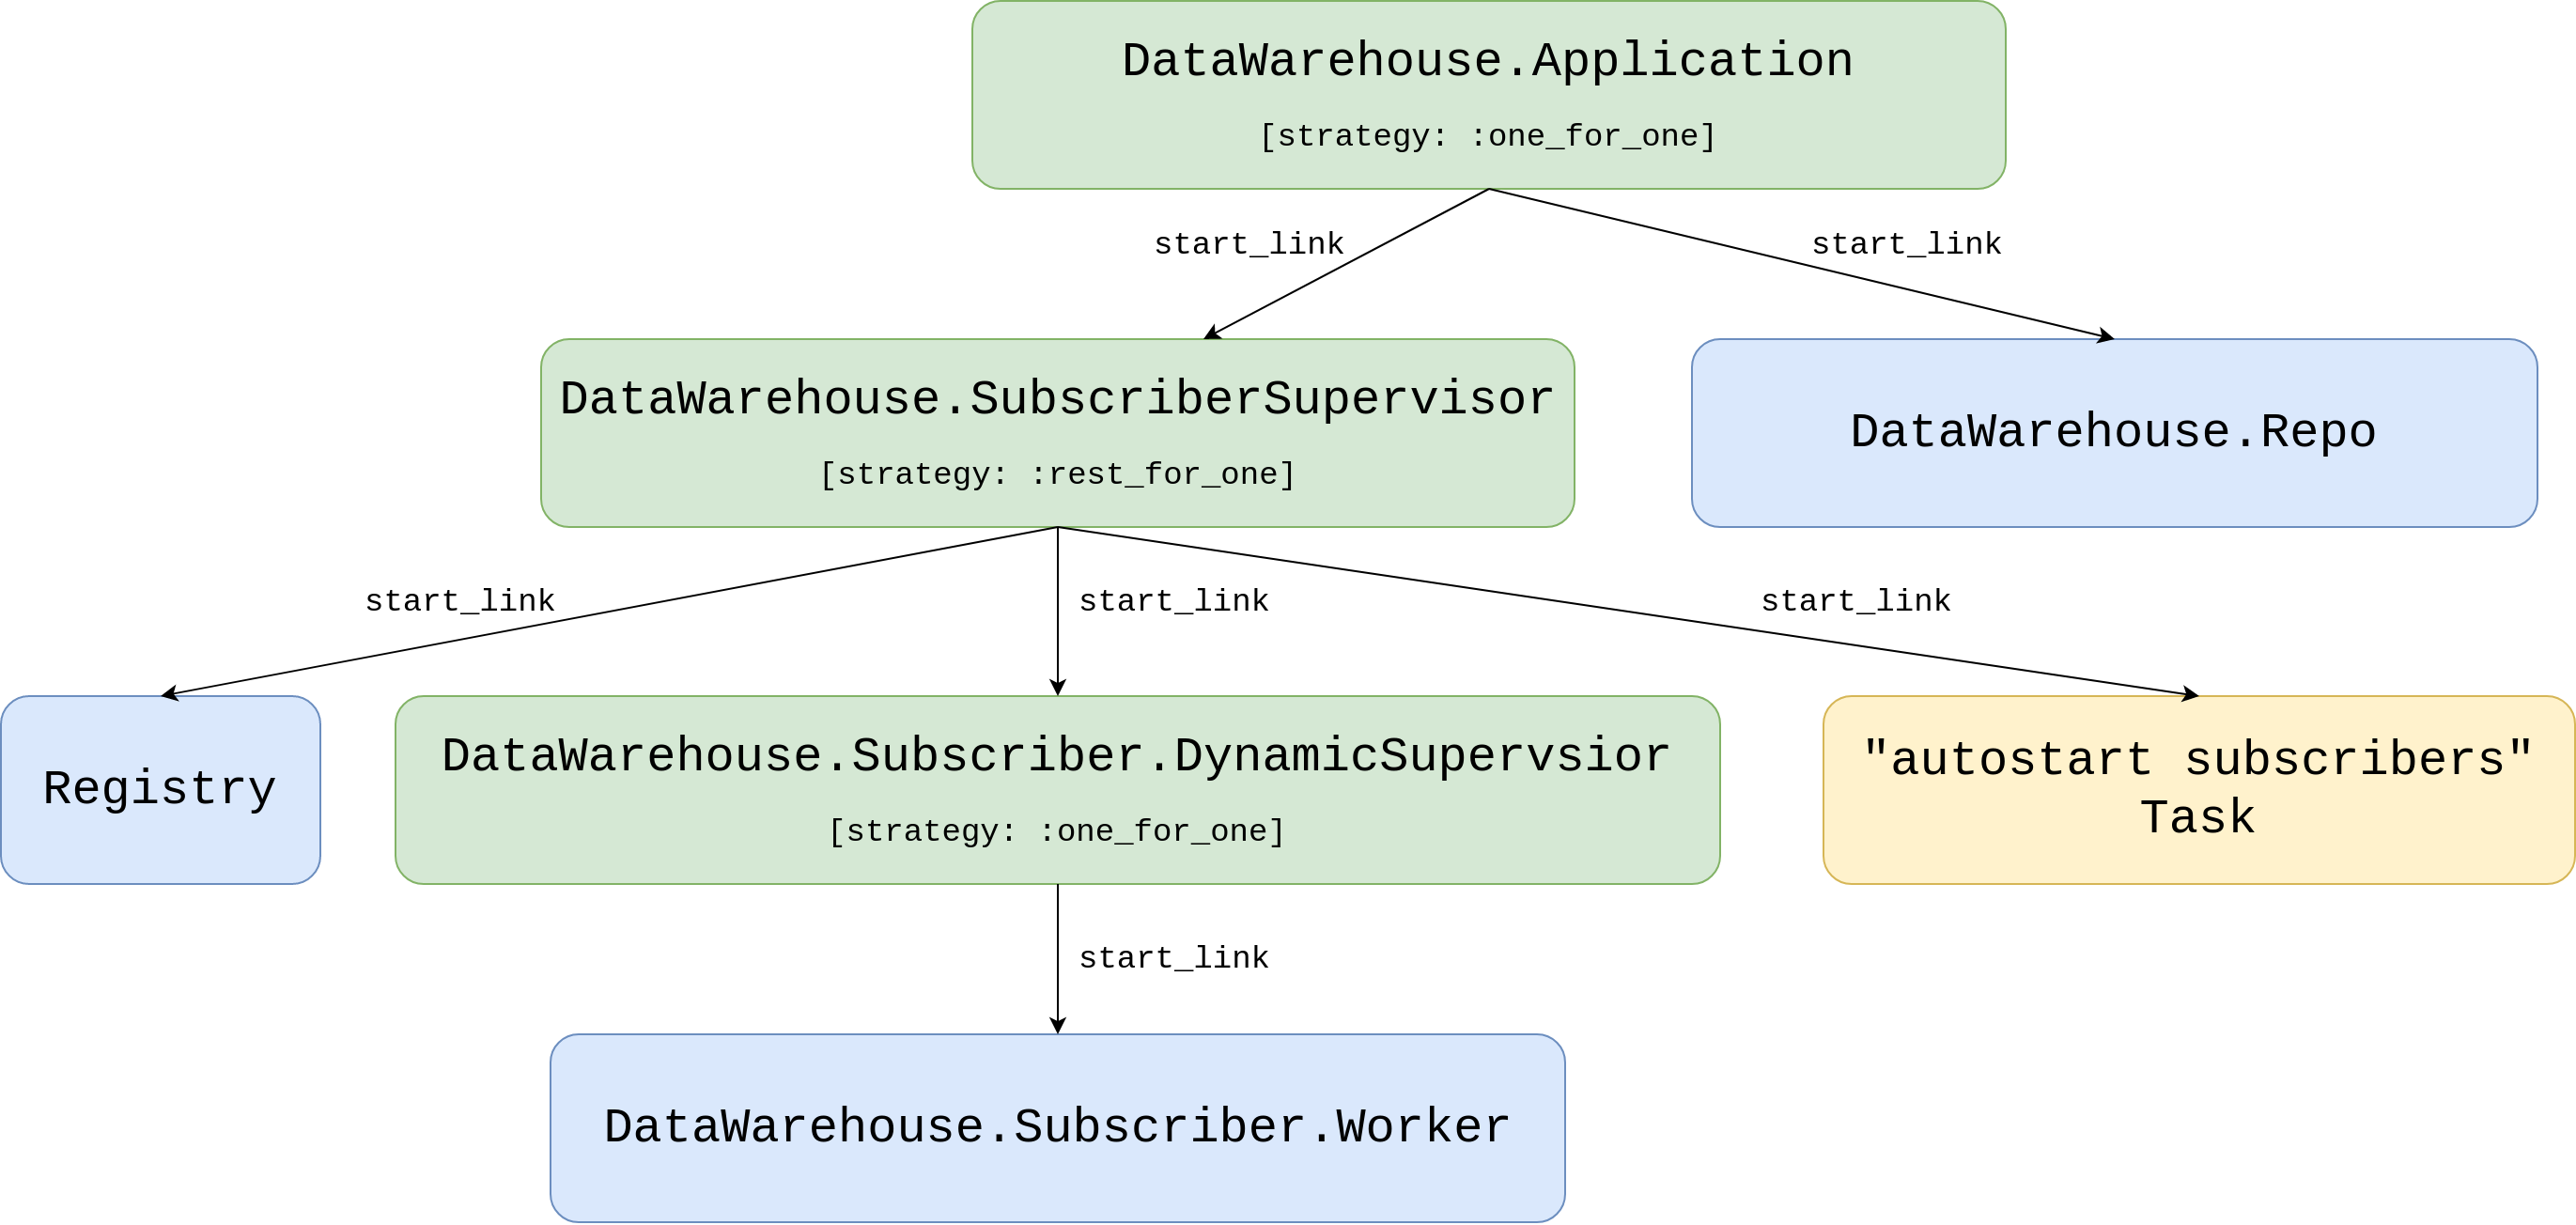
\includegraphics{images/chapter_14_01_sup_diagram.png}
\caption{Supervision tree with Registry}
\end{figure}

Everything looks very similar to the supervision tree that we created in the \texttt{streamer} and the \texttt{naive} applications but there's an additional \texttt{Registry} that is supervised by the \texttt{SubscriberSupervisior} process.

The idea is that inside the \texttt{Worker} module's \texttt{start\_link/1} we will register worker processes using \href{https://hexdocs.pm/elixir/master/GenServer.html\#module-name-registration}{:via} tuple. Internally, GenServer will utilize \texttt{Registry}'s functions like \texttt{register\_name/2} to add process to the registry under the \texttt{topic} string. This way we will be able to retrieve pids assigned to topics using those topic strings instead of registering each worker process with an atom name.

Just as previously the \texttt{DynamicSupervisor} will be in charge of the supervising the \texttt{Worker} processes and it won't be even aware that we are using the \texttt{Registry} to keep track of \texttt{topic\ =\textgreater{}\ pid} association.

\hypertarget{create-the-datawarehouse.subscriber.dynamicsupervisor-module}{%
\subsection{\texorpdfstring{Create the \texttt{DataWarehouse.Subscriber.DynamicSupervisor} module}{Create the DataWarehouse.Subscriber.DynamicSupervisor module}}\label{create-the-datawarehouse.subscriber.dynamicsupervisor-module}}

Let's start by creating a new file called \texttt{dynamic\_supervisor.ex} inside the \texttt{apps/data\_warehouse/lib/data\_warehouse/subscriber} directory and put default dynamic supervisor implementation inside:

\begin{Shaded}
\begin{Highlighting}[]
\CommentTok{\# /apps/data\_warehouse/lib/data\_warehouse/subscriber/dynamic\_supervisor.ex}
\KeywordTok{defmodule} \ConstantTok{DataWarehouse}\OperatorTok{.}\ConstantTok{Subscriber}\OperatorTok{.}\ConstantTok{DynamicSupervisor} \KeywordTok{do}
  \ImportTok{use} \ConstantTok{DynamicSupervisor}

  \KeywordTok{def}\NormalTok{ start\_link(\_arg) }\KeywordTok{do}
    \ConstantTok{DynamicSupervisor}\OperatorTok{.}\NormalTok{start\_link(}\ConstantTok{\_\_MODULE\_\_}\NormalTok{, [], }\VariableTok{name:} \ConstantTok{\_\_MODULE\_\_}\NormalTok{)}
  \KeywordTok{end}

  \KeywordTok{def}\NormalTok{ init(\_arg) }\KeywordTok{do}
    \ConstantTok{DynamicSupervisor}\OperatorTok{.}\NormalTok{init(}\VariableTok{strategy:} \VariableTok{:one\_for\_one}\NormalTok{)}
  \KeywordTok{end}
\KeywordTok{end}
\end{Highlighting}
\end{Shaded}

As we will put all our logic related to autostarting, starting and stopping inside this module we can already add aliases, import and require:

\begin{Shaded}
\begin{Highlighting}[]
\CommentTok{\# /apps/data\_warehouse/lib/data\_warehouse/subscriber/dynamic\_supervisor.ex}
  \ImportTok{require} \ConstantTok{Logger}

  \ImportTok{alias} \ConstantTok{DataWarehouse}\OperatorTok{.}\ConstantTok{Repo}
  \ImportTok{alias} \ConstantTok{DataWarehouse}\OperatorTok{.}\ConstantTok{Schema}\OperatorTok{.}\ConstantTok{SubscriberSettings}
  \ImportTok{alias} \ConstantTok{DataWarehouse}\OperatorTok{.}\ConstantTok{Subscriber}\OperatorTok{.}\ConstantTok{Worker}

  \ImportTok{import} \ConstantTok{Ecto}\OperatorTok{.}\ConstantTok{Query}\NormalTok{, }\VariableTok{only:}\NormalTok{ [}\VariableTok{from:} \DecValTok{2}\NormalTok{]}

  \OtherTok{@registry} \VariableTok{:subscriber\_workers}
\end{Highlighting}
\end{Shaded}

Additionally, we added the \texttt{@registry} module attribute that we will use to retrieve pid for the specific topic.

We can move on to implementing \texttt{autostart\_workers/0} which will look very similar to the ones that we implemented in the \texttt{streamer} and the \texttt{naive} applications:

\begin{Shaded}
\begin{Highlighting}[]
  \CommentTok{\# /apps/data\_warehouse/lib/data\_warehouse/subscriber/dynamic\_supervisor.ex}
  \OperatorTok{...}
  \KeywordTok{def}\NormalTok{ autostart\_workers() }\KeywordTok{do}
    \ConstantTok{Repo}\OperatorTok{.}\NormalTok{all(}
\NormalTok{      from(s }\KeywordTok{in} \ConstantTok{SubscriberSettings}\NormalTok{,}
        \VariableTok{where:}\NormalTok{ s}\OperatorTok{.}\NormalTok{status }\OperatorTok{==} \StringTok{"on"}\NormalTok{,}
        \VariableTok{select:}\NormalTok{ s}\OperatorTok{.}\NormalTok{topic}
\NormalTok{      )}
\NormalTok{    )}
    \OperatorTok{|\textgreater{}} \ConstantTok{Enum}\OperatorTok{.}\NormalTok{map(}\OperatorTok{\&}\NormalTok{start\_child}\OperatorTok{/}\DecValTok{1}\NormalTok{)}
  \KeywordTok{end}

  \KeywordTok{defp}\NormalTok{ start\_child(args) }\KeywordTok{do}
    \ConstantTok{DynamicSupervisor}\OperatorTok{.}\NormalTok{start\_child(}
      \ConstantTok{\_\_MODULE\_\_}\NormalTok{,}
\NormalTok{      \{}\ConstantTok{Worker}\NormalTok{, args\}}
\NormalTok{    )}
  \KeywordTok{end}
\end{Highlighting}
\end{Shaded}

We can see that we are querying the database for list of \texttt{topic}s(not symbols) and we are calling \texttt{start\_child/2} for each results.

The \texttt{start\_worker/1} is where the \texttt{Registry} will shine as we won't need to check is there already a process running for that topic - we can leave that check to the \texttt{Registry}. If there's process already running for that topic it will just return a tuple starting with \texttt{:error} atom:

\begin{Shaded}
\begin{Highlighting}[]
  \CommentTok{\# /apps/data\_warehouse/lib/data\_warehouse/subscriber/dynamic\_supervisor.ex}
  \OperatorTok{...}
  \KeywordTok{def}\NormalTok{ start\_worker(topic) }\KeywordTok{do}
    \ConstantTok{Logger}\OperatorTok{.}\NormalTok{info(}\StringTok{"Starting storing data from }\OtherTok{\#\{}\NormalTok{topic}\OtherTok{\}}\StringTok{ topic"}\NormalTok{)}
\NormalTok{    update\_status(topic, }\StringTok{"on"}\NormalTok{)}
\NormalTok{    start\_child(topic)}
  \KeywordTok{end}
  \OperatorTok{...}
  \KeywordTok{defp}\NormalTok{ update\_status(topic, status)}
       \KeywordTok{when}\NormalTok{ is\_binary(topic) }\KeywordTok{and}\NormalTok{ is\_binary(status) }\KeywordTok{do}
\NormalTok{    \%}\ConstantTok{SubscriberSettings}\NormalTok{\{}
      \VariableTok{topic:}\NormalTok{ topic,}
      \VariableTok{status:}\NormalTok{ status}
\NormalTok{    \}}
    \OperatorTok{|\textgreater{}} \ConstantTok{Repo}\OperatorTok{.}\NormalTok{insert(}
      \VariableTok{on\_conflict:} \VariableTok{:replace\_all}\NormalTok{,}
      \VariableTok{conflict\_target:} \VariableTok{:topic}
\NormalTok{    )}
  \KeywordTok{end}
\end{Highlighting}
\end{Shaded}

As we are not seeding the database with the default settings we will use the \texttt{insert/2} function with options(as previously) to make it work as it would be an ``upsert'' function.

Last function in this module will be \texttt{stop\_worker/1} which uses private \texttt{stop\_child/1} function. The \texttt{stop\_child/1} function shows how to retrieve \texttt{pid} of the process assigned to the passed \texttt{topic}:

\begin{Shaded}
\begin{Highlighting}[]
  \CommentTok{\# /apps/data\_warehouse/lib/data\_warehouse/subscriber/dynamic\_supervisor.ex}
  \OperatorTok{...}
  \KeywordTok{def}\NormalTok{ stop\_worker(topic) }\KeywordTok{do}
    \ConstantTok{Logger}\OperatorTok{.}\NormalTok{info(}\StringTok{"Stopping storing data from }\OtherTok{\#\{}\NormalTok{topic}\OtherTok{\}}\StringTok{ topic"}\NormalTok{)}
\NormalTok{    update\_status(topic, }\StringTok{"off"}\NormalTok{)}
\NormalTok{    stop\_child(topic)}
  \KeywordTok{end}
  \OperatorTok{...}
  \KeywordTok{defp}\NormalTok{ stop\_child(args) }\KeywordTok{do}
    \KeywordTok{case} \ConstantTok{Registry}\OperatorTok{.}\NormalTok{lookup(}\OtherTok{@registry}\NormalTok{, args) }\KeywordTok{do}
\NormalTok{      [\{pid, \_\}] }\OperatorTok{{-}\textgreater{}} \ConstantTok{DynamicSupervisor}\OperatorTok{.}\NormalTok{terminate\_child(}\ConstantTok{\_\_MODULE\_\_}\NormalTok{, pid)}
\NormalTok{      \_ }\OperatorTok{{-}\textgreater{}} \ConstantTok{Logger}\OperatorTok{.}\NormalTok{warn(}\StringTok{"Unable to locate process assigned to }\OtherTok{\#\{}\NormalTok{inspect(args)}\OtherTok{\}}\StringTok{"}\NormalTok{)}
    \KeywordTok{end}
  \KeywordTok{end}
\end{Highlighting}
\end{Shaded}

That is a full implementation of the \texttt{DataWarehouse.Subscriber.DynamicSupervisor} module and it's almost as slim as one from the last chapter where we leveraged macros to achieve that lightness. Using the \texttt{Registry} is the preferred way to manage a list of identifiable processes. We won't run into an issue of overusing the atoms(as they are not garbage collected, we could hit that limit sooner or later).

\hypertarget{register-worker-processes-using-via}{%
\subsection{Register Worker processes using :via}\label{register-worker-processes-using-via}}

The above \texttt{DynamicSupervisor} module assumes that Workers are registered inside the \texttt{Registry} - to make this happen we will need to update the \texttt{start\_link/1} function of the \texttt{DataWarehouse.Subscriber.Worker} module:

\begin{Shaded}
\begin{Highlighting}[]
  \CommentTok{\# /apps/data\_warehouse/lib/data\_warehouse/subscriber/worker.ex}
  \OperatorTok{...}
  \KeywordTok{def}\NormalTok{ start\_link(topic) }\KeywordTok{do}
    \ConstantTok{GenServer}\OperatorTok{.}\NormalTok{start\_link(}
      \ConstantTok{\_\_MODULE\_\_}\NormalTok{,}
\NormalTok{      topic,}
      \VariableTok{name:}\NormalTok{ via\_tuple(topic)}
\NormalTok{    )}
  \KeywordTok{end}
  \OperatorTok{...}
  \KeywordTok{defp}\NormalTok{ via\_tuple(topic) }\KeywordTok{do}
\NormalTok{    \{}\VariableTok{:via}\NormalTok{, }\ConstantTok{Registry}\NormalTok{, \{}\VariableTok{:subscriber\_workers}\NormalTok{, topic\}\}}
  \KeywordTok{end}
  \OperatorTok{...}    
\end{Highlighting}
\end{Shaded}

Passing the \texttt{:name} option to the \texttt{GenServer}'s \texttt{start\_link/3} function we instruct it to utilize the \texttt{Registry} module to register processes under topic names.

\hypertarget{create-a-new-supervision-level-for-registry-task-and-the-dynamicsupervisor}{%
\subsection{Create a new supervision level for Registry, Task and the DynamicSupervisor}\label{create-a-new-supervision-level-for-registry-task-and-the-dynamicsupervisor}}

We have the lowest level modules - the \texttt{Worker} and the \texttt{DynamicSupervisor} implemented - time to add a new \texttt{Supervisor} that will start the \texttt{Registry}, the \texttt{DynamicSupervisor} and the autostart storing \texttt{Task}. First create a new file called \texttt{subscriber\_supervisor.ex} inside the \texttt{apps/data\_warehouse/lib/data\_warehouse} directory:

\begin{Shaded}
\begin{Highlighting}[]
\CommentTok{\# /apps/data\_warehouse/lib/data\_warehouse/subscriber\_supervisor.ex}
\KeywordTok{defmodule} \ConstantTok{DataWarehouse}\OperatorTok{.}\ConstantTok{SubscriberSupervisor} \KeywordTok{do}
  \ImportTok{use} \ConstantTok{Supervisor}

  \ImportTok{alias} \ConstantTok{DataWarehouse}\OperatorTok{.}\ConstantTok{Subscriber}\OperatorTok{.}\ConstantTok{DynamicSupervisor}

  \OtherTok{@registry} \VariableTok{:subscriber\_workers}

  \KeywordTok{def}\NormalTok{ start\_link(\_args) }\KeywordTok{do}
    \ConstantTok{Supervisor}\OperatorTok{.}\NormalTok{start\_link(}\ConstantTok{\_\_MODULE\_\_}\NormalTok{, [], }\VariableTok{name:} \ConstantTok{\_\_MODULE\_\_}\NormalTok{)}
  \KeywordTok{end}

  \KeywordTok{def}\NormalTok{ init(\_args) }\KeywordTok{do}
\NormalTok{    children }\OperatorTok{=}\NormalTok{ [}
\NormalTok{      \{}\ConstantTok{Registry}\NormalTok{, [}\VariableTok{keys:} \VariableTok{:unique}\NormalTok{, }\VariableTok{name:} \OtherTok{@registry}\NormalTok{]\},}
\NormalTok{      \{}\ConstantTok{DynamicSupervisor}\NormalTok{, []\},}
\NormalTok{      \{}\ConstantTok{Task}\NormalTok{,}
       \KeywordTok{fn} \OperatorTok{{-}\textgreater{}}
         \ConstantTok{DynamicSupervisor}\OperatorTok{.}\NormalTok{autostart\_workers()}
       \KeywordTok{end}\NormalTok{\}}
\NormalTok{    ]}

    \ConstantTok{Supervisor}\OperatorTok{.}\NormalTok{init(children, }\VariableTok{strategy:} \VariableTok{:rest\_for\_one}\NormalTok{)}
  \KeywordTok{end}
\KeywordTok{end}
\end{Highlighting}
\end{Shaded}

Important part here will be to match the \texttt{Registry} name to the one defined inside the \texttt{DynamicSupervisor} and the \texttt{Worker} modules.

\hypertarget{link-the-subscribersupervisor-to-the-application}{%
\subsection{\texorpdfstring{Link the \texttt{SubscriberSupervisor} to the \texttt{Application}}{Link the SubscriberSupervisor to the Application}}\label{link-the-subscribersupervisor-to-the-application}}

We need to update the \texttt{DataWarehouse.Application} module to start our new \texttt{DataWarehouse.SubscriberSupervisor} process as well as register itself under name matching to its module(just for consistency with other applications):

\begin{Shaded}
\begin{Highlighting}[]
  \CommentTok{\# /apps/data\_warehouse/lib/data\_warehouse/application.ex}
  \OperatorTok{...}
  \KeywordTok{def}\NormalTok{ start(\_type, \_args) }\KeywordTok{do}
\NormalTok{    children }\OperatorTok{=}\NormalTok{ [}
\NormalTok{      \{}\ConstantTok{DataWarehouse}\OperatorTok{.}\ConstantTok{Repo}\NormalTok{, []\},}
\NormalTok{      \{}\ConstantTok{DataWarehouse}\OperatorTok{.}\ConstantTok{SubscriberSupervisor}\NormalTok{, []\} }\CommentTok{\# \textless{}= new module added}
\NormalTok{    ]}

    \CommentTok{\# See https://hexdocs.pm/elixir/Supervisor.html}
    \CommentTok{\# for other strategies and supported options}
\NormalTok{    opts }\OperatorTok{=}\NormalTok{ [}\VariableTok{strategy:} \VariableTok{:one\_for\_one}\NormalTok{, }\VariableTok{name:} \ConstantTok{\_\_MODULE\_\_}\NormalTok{] }\CommentTok{\# \textless{}= name updated}
    \ConstantTok{Supervisor}\OperatorTok{.}\NormalTok{start\_link(children, opts)}
  \KeywordTok{end}
  \OperatorTok{...}
\end{Highlighting}
\end{Shaded}

\hypertarget{add-interface}{%
\subsection{Add interface}\label{add-interface}}

The final step will be to add an interface to the \texttt{DataWarehouse} application to start and stop storing:

\begin{Shaded}
\begin{Highlighting}[]
  \CommentTok{\# /apps/data\_warehouse/lib/data\_warehouse.ex}
  \ImportTok{alias} \ConstantTok{DataWarehouse}\OperatorTok{.}\ConstantTok{Subscriber}\OperatorTok{.}\ConstantTok{DynamicSupervisor}

  \KeywordTok{def}\NormalTok{ start\_storing(stream, symbol) }\KeywordTok{do}
\NormalTok{    to\_topic(stream, symbol)}
    \OperatorTok{|\textgreater{}} \ConstantTok{DynamicSupervisor}\OperatorTok{.}\NormalTok{start\_worker()}
  \KeywordTok{end}

  \KeywordTok{def}\NormalTok{ stop\_storing(stream, symbol) }\KeywordTok{do}
\NormalTok{    to\_topic(stream, symbol)}
    \OperatorTok{|\textgreater{}} \ConstantTok{DynamicSupervisor}\OperatorTok{.}\NormalTok{stop\_worker()}
  \KeywordTok{end}

  \KeywordTok{defp}\NormalTok{ to\_topic(stream, symbol) }\KeywordTok{do}
\NormalTok{    [stream, symbol]}
    \OperatorTok{|\textgreater{}} \ConstantTok{Enum}\OperatorTok{.}\NormalTok{map(}\OperatorTok{\&}\ConstantTok{String}\OperatorTok{.}\NormalTok{upcase}\OperatorTok{/}\DecValTok{1}\NormalTok{)}
    \OperatorTok{|\textgreater{}} \ConstantTok{Enum}\OperatorTok{.}\NormalTok{join(}\StringTok{":"}\NormalTok{)}
  \KeywordTok{end}
\end{Highlighting}
\end{Shaded}

Inside the above functions, we are just doing a couple of sanity checks on the case of the passed arguments assuming that both topics and stream are uppercase.

\hypertarget{test}{%
\subsection{Test}\label{test}}

The interface above was the last step in our implementation, we can now test that all works as expected:

\begin{Shaded}
\begin{Highlighting}[]
\ExtensionTok{$}\NormalTok{ iex }\AttributeTok{{-}S}\NormalTok{ mix}
\ExtensionTok{...}
\ExtensionTok{iex}\ErrorTok{(}\ExtensionTok{1}\KeywordTok{)}\OperatorTok{\textgreater{}}\NormalTok{ DataWarehouse.start\_storing}\KeywordTok{(}\StringTok{"TRADE\_EVENTS"}\ExtensionTok{,} \StringTok{"NEOUSDT"}\KeywordTok{)}
\ExtensionTok{19:34:00.740}\NormalTok{ [info]  Starting storing data from TRADE\_EVENTS:NEOUSDT topic}
\ExtensionTok{19:34:00.847}\NormalTok{ [info]  DataWarehouse worker is subscribing to TRADE\_EVENTS:NEOUSDT}
\ExtensionTok{\{:ok,} \CommentTok{\#PID\textless{}0.429.0\textgreater{}\}}
\ExtensionTok{iex}\ErrorTok{(}\ExtensionTok{2}\KeywordTok{)}\OperatorTok{\textgreater{}}\NormalTok{ DataWarehouse.start\_storing}\KeywordTok{(}\StringTok{"TRADE\_EVENTS"}\ExtensionTok{,} \StringTok{"NEOUSDT"}\KeywordTok{)}
\ExtensionTok{19:34:04.753}\NormalTok{ [info]  Starting storing data from TRADE\_EVENTS:NEOUSDT topic}
\ExtensionTok{\{:error,}\NormalTok{ \{:already\_started, }\CommentTok{\#PID\textless{}0.459.0\textgreater{}\}\}}
\ExtensionTok{iex}\ErrorTok{(}\ExtensionTok{3}\KeywordTok{)}\OperatorTok{\textgreater{}}\NormalTok{ DataWarehouse.start\_storing}\KeywordTok{(}\StringTok{"ORDERS"}\ExtensionTok{,} \StringTok{"NEOUSDT"}\KeywordTok{)}
\ExtensionTok{19:34:09.386}\NormalTok{ [info]  Starting storing data from ORDERS:NEOUSDT topic}
\ExtensionTok{19:34:09.403}\NormalTok{ [info]  DataWarehouse worker is subscribing to ORDERS:NEOUSDT}
\ExtensionTok{\{:ok,} \CommentTok{\#PID\textless{}0.431.0\textgreater{}\}}
\ExtensionTok{BREAK:} \ErrorTok{(}\ExtensionTok{a}\KeywordTok{)}\ExtensionTok{bort} \ErrorTok{(}\ExtensionTok{A}\KeywordTok{)}\ExtensionTok{bort}\NormalTok{ with dump }\ErrorTok{(}\ExtensionTok{c}\KeywordTok{)}\ExtensionTok{ontinue} \ErrorTok{(}\ExtensionTok{p}\KeywordTok{)}\ExtensionTok{roc}\NormalTok{ info }\ErrorTok{(}\ExtensionTok{i}\KeywordTok{)}\ExtensionTok{nfo}
       \KeywordTok{(}\ExtensionTok{l}\KeywordTok{)}\ExtensionTok{oaded} \ErrorTok{(}\ExtensionTok{v}\KeywordTok{)}\ExtensionTok{ersion} \ErrorTok{(}\ExtensionTok{k}\KeywordTok{)}\ExtensionTok{ill} \ErrorTok{(}\ExtensionTok{D}\KeywordTok{)}\ExtensionTok{b{-}tables} \ErrorTok{(}\ExtensionTok{d}\KeywordTok{)}\ExtensionTok{istribution}
\ExtensionTok{\^{}C\%}
\ExtensionTok{$}\NormalTok{ iex }\AttributeTok{{-}S}\NormalTok{ mix}
\ExtensionTok{...}
\ExtensionTok{19:35:30.058}\NormalTok{ [info]  DataWarehouse worker is subscribing to TRADE\_EVENTS:NEOUSDT}
\ExtensionTok{19:35:30.062}\NormalTok{ [info]  DataWarehouse worker is subscribing to ORDERS:NEOUSDT}
\CommentTok{\# autostart works \^{}\^{}\^{}}
\ExtensionTok{iex}\ErrorTok{(}\ExtensionTok{1}\KeywordTok{)}\OperatorTok{\textgreater{}}\NormalTok{ Naive.start\_trading}\KeywordTok{(}\StringTok{"NEOUSDT"}\KeywordTok{)}
\ExtensionTok{19:36:45.316}\NormalTok{ [info]  Starting Elixir.Naive.SymbolSupervisor worker for NEOUSDT}
\ExtensionTok{19:36:45.417}\NormalTok{ [info]  Starting new supervision tree to trade on NEOUSDT}
\ExtensionTok{\{:ok,} \CommentTok{\#PID\textless{}0.419.0\textgreater{}\}}
\ExtensionTok{iex}\ErrorTok{(}\ExtensionTok{3}\KeywordTok{)}\OperatorTok{\textgreater{}} 
\ExtensionTok{19:36:47.484}\NormalTok{ [info]  Initializing new trader}\ErrorTok{(}\ExtensionTok{1615221407466}\KeywordTok{)} \ControlFlowTok{for}\NormalTok{ NEOUSDT}
\ExtensionTok{iex}\ErrorTok{(}\ExtensionTok{2}\KeywordTok{)}\OperatorTok{\textgreater{}}\NormalTok{ Streamer.start\_streaming}\KeywordTok{(}\StringTok{"NEOUSDT"}\KeywordTok{)}
\ExtensionTok{16:37:39.660}\NormalTok{ [info]  Starting Elixir.Streamer.Binance worker for NEOUSDT}
\ExtensionTok{\{:ok,} \CommentTok{\#PID\textless{}0.428.0\textgreater{}\}}
\ExtensionTok{...}
\ExtensionTok{iex}\ErrorTok{(}\ExtensionTok{3}\KeywordTok{)}\OperatorTok{\textgreater{}}\NormalTok{ DataWarehouse.stop\_storing}\KeywordTok{(}\StringTok{"trade\_events"}\ExtensionTok{,} \StringTok{"NEOUSDT"}\KeywordTok{)}
\ExtensionTok{19:39:26.398}\NormalTok{ [info]  Stopping storing data from trade\_events:NEOUSDT topic}
\ExtensionTok{:ok}
\ExtensionTok{iex}\ErrorTok{(}\ExtensionTok{4}\KeywordTok{)}\OperatorTok{\textgreater{}}\NormalTok{ DataWarehouse.stop\_storing}\KeywordTok{(}\StringTok{"trade\_events"}\ExtensionTok{,} \StringTok{"NEOUSDT"}\KeywordTok{)}
\ExtensionTok{19:39:28.151}\NormalTok{ [info]  Stopping storing data from trade\_events:NEOUSDT topic}
\ExtensionTok{19:39:28.160}\NormalTok{ [warn]  Unable to locate process assigned to }\StringTok{"trade\_events:NEOUSDT"}
\ExtensionTok{:ok}
\ExtensionTok{iex}\ErrorTok{(}\ExtensionTok{5}\KeywordTok{)}\OperatorTok{\textgreater{}}\NormalTok{ [\{pid, }\ExtensionTok{nil\}]}\NormalTok{ = Registry.lookup}\ErrorTok{(}\ExtensionTok{:subscriber\_workers,} \StringTok{"ORDERS:NEOUSDT"}\KeywordTok{)}
\ExtensionTok{[\{\#PID}\OperatorTok{\textless{}}\NormalTok{0.417.0}\OperatorTok{\textgreater{}}\NormalTok{, nil\}]}
\ExtensionTok{iex}\ErrorTok{(}\ExtensionTok{6}\KeywordTok{)}\OperatorTok{\textgreater{}}\NormalTok{ Process.exit}\KeywordTok{(}\ExtensionTok{pid,}\NormalTok{ :crash}\KeywordTok{)}
\FunctionTok{true}
\ExtensionTok{16:43:40.812}\NormalTok{ [info]  DataWarehouse worker is subscribing to ORDERS:NEOUSDT}
\end{Highlighting}
\end{Shaded}

As we can see even this simple implementation handles starting, autostarting and stopping. It also gracefully handles starting workers when one is already running as well as stopping when there none running.

As a challenge, you could update the \texttt{naive} and the \texttt{streamer} application to use \texttt{Registry} and remove \texttt{Core.ServiceSupervisor} module as it was superseded by the above solution.

{[}Note{]} Please remember to run \texttt{mix\ format} to keep things nice and tidy.

Source code for this chapter can be found at \href{https://github.com/frathon/create-a-cryptocurrency-trading-bot-in-elixir-source-code/tree/chapter_14}{Github}

\hypertarget{backtest-trading-strategy}{%
\chapter{Backtest trading strategy}\label{backtest-trading-strategy}}

\hypertarget{objectives-14}{%
\section{Objectives}\label{objectives-14}}

\begin{itemize}
\tightlist
\item
  overview of requirements
\item
  implement the storing task
\item
  test the backtesting
\end{itemize}

\hypertarget{overview-of-requirements-2}{%
\section{Overview of requirements}\label{overview-of-requirements-2}}

In the last chapter, we started storing trade events and orders in the database which will be crucial for backtesting, which we will focus on in this chapter.

Backtesting is a procedure of running historical data through the system and observing how our strategy would perform as if we would run it ``in the past''. Backtesting works on assumption that the market will behave in a similar fashion in the future as it was in the past.

At this moment we are receiving the trade events from the Binance through WebSocket. The \texttt{Streamer.Binance} process is handling those messages by parsing them from JSON string to map, then converting them to structs and broadcasting them to the \texttt{TRADE\_EVENTS:\#\{symbol\}} PubSub topic. The \texttt{Naive.Trader} subscribes to the \texttt{TRADE\_EVENTS:\#\{symbol\}} topic and takes decisions based on incoming data. As it places buy and sell orders it broadcasts them to the \texttt{ORDERS:\#\{symbol\}} PubSub topic. The \texttt{DataWarehouse.Subscriber.Worker} processes subscribe to both trade events and orders topics and store incoming data inside the database - we can visualize that flow like that:

\begin{figure}
\centering
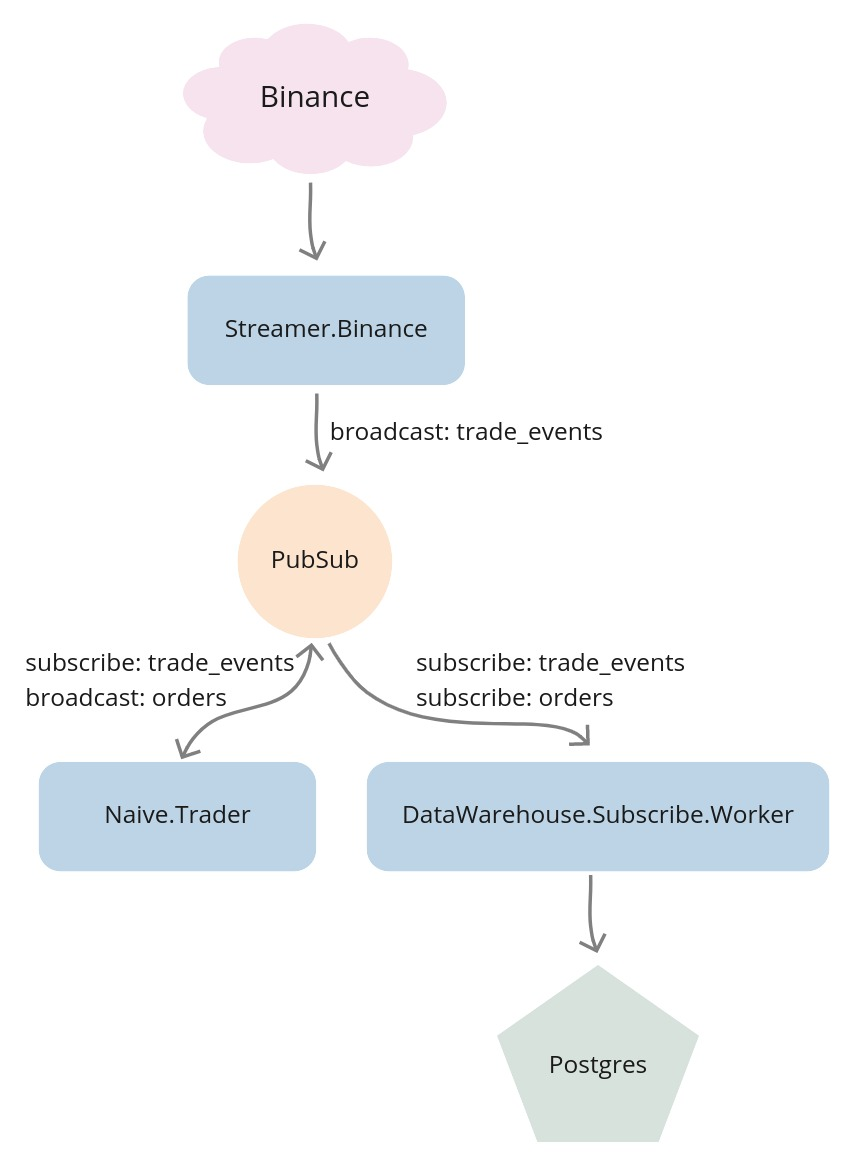
\includegraphics{images/chapter_14_02_current_pubsub.png}
\caption{Normal broadcast/subscribe flow}
\end{figure}

To backtest we can substitute the \texttt{Streamer.Binance} process with a \texttt{Task} that will \texttt{stream} trade events' data from the database and broadcasts it to the \texttt{TRADE\_EVENTS:\#\{symbol\}} PubSub topic(the same topic as the \texttt{Streamer.Binance} process).

From the perspective of the \texttt{Naive.Trader} it \emph{does not} make any difference who is broadcasting those trade events. This should be a clear indication of the value of publish/subscribe model that we implemented from the beginning. It allows us to swap producer and consumers freely to backtest our trading strategies:

\begin{figure}
\centering
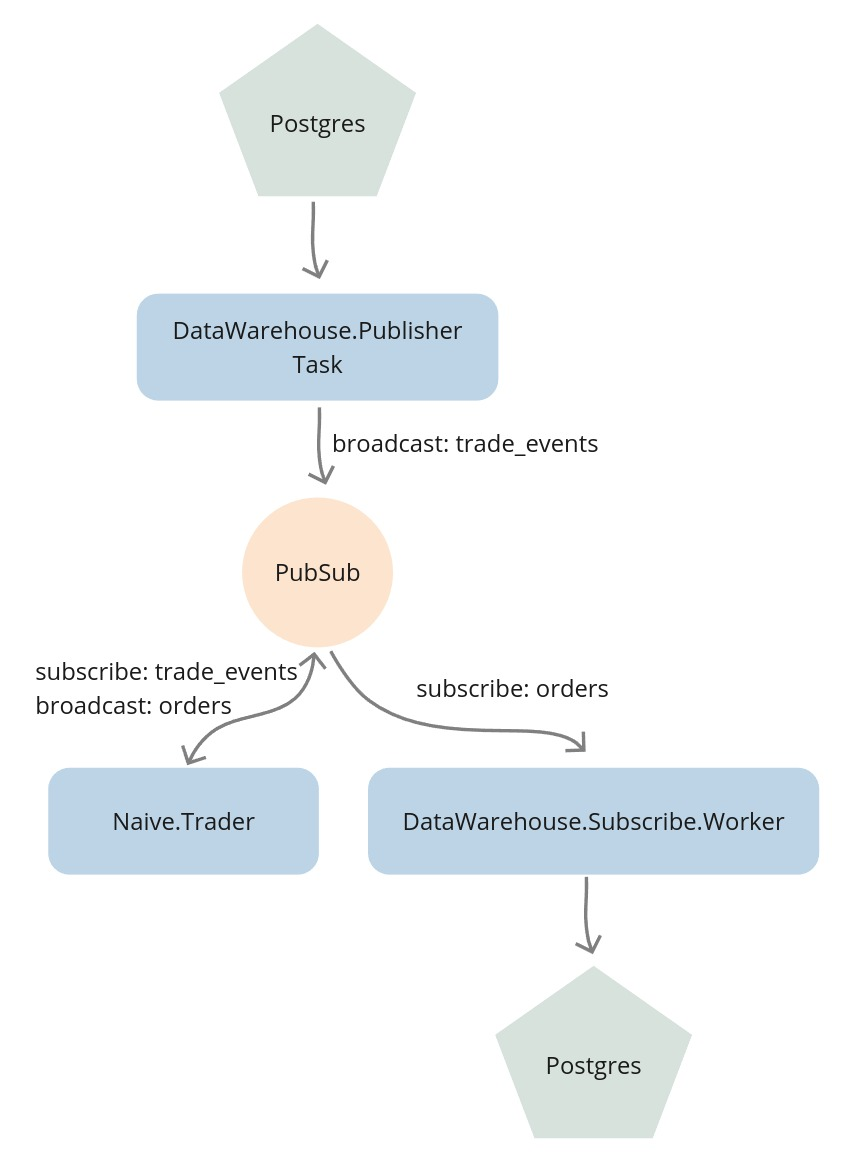
\includegraphics{images/chapter_14_03_backtest_pubsub.png}
\caption{Task feeds the stream of data from the database straight to the PubSub topic}
\end{figure}

\hypertarget{implement-the-storing-task}{%
\section{Implement the storing task}\label{implement-the-storing-task}}

We will start by creating a new file called \texttt{publisher.ex} inside the \texttt{apps/data\_warehouse/lib/data\_warehouse} directory. We will start by implementing the basic \texttt{Task} behavior:

\begin{Shaded}
\begin{Highlighting}[]
\CommentTok{\# /apps/data\_warehouse/lib/data\_warehouse/publisher.ex}
\KeywordTok{defmodule} \ConstantTok{DataWarehouse}\OperatorTok{.}\ConstantTok{Publisher} \KeywordTok{do}
  \ImportTok{use} \ConstantTok{Task}

  \KeywordTok{def}\NormalTok{ start\_link(arg) }\KeywordTok{do}
    \ConstantTok{Task}\OperatorTok{.}\NormalTok{start\_link(}\ConstantTok{\_\_MODULE\_\_}\NormalTok{, }\VariableTok{:run}\NormalTok{, [arg])}
  \KeywordTok{end}

  \KeywordTok{def}\NormalTok{ run(arg) }\KeywordTok{do}
    \CommentTok{\# ...}
  \KeywordTok{end}
\KeywordTok{end}
\end{Highlighting}
\end{Shaded}

To be able to query the database we will import \texttt{Ecto} and require \texttt{Logger} for logging:

\begin{Shaded}
\begin{Highlighting}[]
  \CommentTok{\# /apps/data\_warehouse/lib/data\_warehouse/publisher.ex}
  \OperatorTok{...}
  \ImportTok{import} \ConstantTok{Ecto}\OperatorTok{.}\ConstantTok{Query}\NormalTok{, }\VariableTok{only:}\NormalTok{ [}\VariableTok{from:} \DecValTok{2}\NormalTok{]}

  \ImportTok{require} \ConstantTok{Logger}
  \OperatorTok{...}
\end{Highlighting}
\end{Shaded}

We can now modify the \texttt{run/1} function to expect specific \texttt{type}, \texttt{symbol}, \texttt{from}, \texttt{to} and \texttt{interval}:

\begin{Shaded}
\begin{Highlighting}[]
  \CommentTok{\# /apps/data\_warehouse/lib/data\_warehouse/publisher.ex  }
  \OperatorTok{...}
  \KeywordTok{def}\NormalTok{ run(\%\{}
        \VariableTok{type:} \VariableTok{:trade\_events}\NormalTok{,}
        \VariableTok{symbol:}\NormalTok{ symbol,}
        \VariableTok{from:}\NormalTok{ from,}
        \VariableTok{to:}\NormalTok{ to,}
        \VariableTok{interval:}\NormalTok{ interval}
\NormalTok{      \}) }\KeywordTok{do}
    \OperatorTok{...}  
\end{Highlighting}
\end{Shaded}

Inside the body of the \texttt{run/1} function, first, we will convert \texttt{from} and \texttt{to} Unix timestamps by using private helper functions as well as make sure that the passed symbol is uppercase:

\begin{Shaded}
\begin{Highlighting}[]
  \CommentTok{\# /apps/data\_warehouse/lib/data\_warehouse/publisher.ex  }
  \OperatorTok{...}
  \KeywordTok{def}\NormalTok{ run(\%\{}
        \OperatorTok{...}
\NormalTok{      \}) }\KeywordTok{do}
\NormalTok{    symbol }\OperatorTok{=} \ConstantTok{String}\OperatorTok{.}\NormalTok{upcase(symbol)}

\NormalTok{    from\_ts }\OperatorTok{=}
      \StringTok{"}\OtherTok{\#\{}\NormalTok{from}\OtherTok{\}}\StringTok{T00:00:00.000Z"}
      \OperatorTok{|\textgreater{}}\NormalTok{ convert\_to\_ms()}

\NormalTok{    to\_ts }\OperatorTok{=}
      \StringTok{"}\OtherTok{\#\{}\NormalTok{to}\OtherTok{\}}\StringTok{T23:59:59.000Z"}
      \OperatorTok{|\textgreater{}}\NormalTok{ convert\_to\_ms()}
  \KeywordTok{end}
  \OperatorTok{...}
  \KeywordTok{defp}\NormalTok{ convert\_to\_ms(iso8601DateString) }\KeywordTok{do}
\NormalTok{    iso8601DateString}
    \OperatorTok{|\textgreater{}} \ConstantTok{NaiveDateTime}\OperatorTok{.}\NormalTok{from\_iso8601!()}
    \OperatorTok{|\textgreater{}} \ConstantTok{DateTime}\OperatorTok{.}\NormalTok{from\_naive!(}\StringTok{"Etc/UTC"}\NormalTok{)}
    \OperatorTok{|\textgreater{}} \ConstantTok{DateTime}\OperatorTok{.}\NormalTok{to\_unix()}
    \OperatorTok{|\textgreater{}} \ConstantTok{Kernel}\OperatorTok{.*}\NormalTok{(}\DecValTok{1000}\NormalTok{)}
  \KeywordTok{end}
\end{Highlighting}
\end{Shaded}

Next, we will select data from the database but because of possibly hundreds of thousands of rows being selected and because we are broadcasting them to the PubSub every x ms it could take a substantial amount of time to \texttt{broadcast} all of them. Instead of \texttt{select}ing data and storing all of it in the memory, we will use \texttt{Repo.stream/1} function to keep \texttt{broadcast}ing it on the go. Additionally, we will add \texttt{index} to the data to be able to log info messages every 10k messages. The last thing that we need to define will be the timeout value - the default value is 5 seconds and we will change it to \texttt{:infinity}:

\begin{Shaded}
\begin{Highlighting}[]
  \CommentTok{\# /apps/data\_warehouse/lib/data\_warehouse/publisher.ex}
  \KeywordTok{def}\NormalTok{ run(\%\{}
        \OperatorTok{...}
\NormalTok{      \}) }\KeywordTok{do}
    \OperatorTok{...}

    \ConstantTok{DataWarehouse}\OperatorTok{.}\ConstantTok{Repo}\OperatorTok{.}\NormalTok{transaction(}
      \KeywordTok{fn} \OperatorTok{{-}\textgreater{}}
\NormalTok{        from(te }\KeywordTok{in} \ConstantTok{DataWarehouse}\OperatorTok{.}\ConstantTok{Schema}\OperatorTok{.}\ConstantTok{TradeEvent}\NormalTok{,}
          \VariableTok{where:}
\NormalTok{            te}\OperatorTok{.}\NormalTok{symbol }\OperatorTok{==} \OperatorTok{\^{}}\NormalTok{symbol }\KeywordTok{and}
\NormalTok{              te}\OperatorTok{.}\NormalTok{trade\_time }\OperatorTok{\textgreater{}=} \OperatorTok{\^{}}\NormalTok{from\_ts }\KeywordTok{and}
\NormalTok{              te}\OperatorTok{.}\NormalTok{trade\_time }\OperatorTok{\textless{}} \OperatorTok{\^{}}\NormalTok{to\_ts,}
          \VariableTok{order\_by:}\NormalTok{ te}\OperatorTok{.}\NormalTok{trade\_time}
\NormalTok{        )}
        \OperatorTok{|\textgreater{}} \ConstantTok{DataWarehouse}\OperatorTok{.}\ConstantTok{Repo}\OperatorTok{.}\NormalTok{stream()}
        \OperatorTok{|\textgreater{}} \ConstantTok{Enum}\OperatorTok{.}\NormalTok{with\_index()}
        \OperatorTok{|\textgreater{}} \ConstantTok{Enum}\OperatorTok{.}\NormalTok{map(}\KeywordTok{fn}\NormalTok{ \{row, index\} }\OperatorTok{{-}\textgreater{}}
          \VariableTok{:timer}\OperatorTok{.}\NormalTok{sleep(interval)}

          \ControlFlowTok{if}\NormalTok{ rem(index, }\DecValTok{10\_000}\NormalTok{) }\OperatorTok{==} \DecValTok{0} \KeywordTok{do}
            \ConstantTok{Logger}\OperatorTok{.}\NormalTok{info(}\StringTok{"Publisher broadcasted }\OtherTok{\#\{}\NormalTok{index}\OtherTok{\}}\StringTok{ events"}\NormalTok{)}
          \KeywordTok{end}

\NormalTok{          publishTradeEvent(row)}
        \KeywordTok{end}\NormalTok{)}
      \KeywordTok{end}\NormalTok{,}
      \VariableTok{timeout:} \VariableTok{:infinity}
\NormalTok{    )}

    \ConstantTok{Logger}\OperatorTok{.}\NormalTok{info(}\StringTok{"Publisher finished streaming trade events"}\NormalTok{)}
  \KeywordTok{end}
\end{Highlighting}
\end{Shaded}

Finally, the above code uses the \texttt{publishTradeEvent/1} helper function which converts DataWarehouse's TradeEvent to the Stremer's TradeEvent to broadcast the same structs as the \texttt{streamer} application:

\begin{Shaded}
\begin{Highlighting}[]
  \CommentTok{\# /apps/data\_warehouse/lib/data\_warehouse/publisher.ex}
  \OperatorTok{...}
  \KeywordTok{defp}\NormalTok{ publishTradeEvent(\%}\ConstantTok{DataWarehouse}\OperatorTok{.}\ConstantTok{Schema}\OperatorTok{.}\ConstantTok{TradeEvent}\NormalTok{\{\} }\OperatorTok{=}\NormalTok{ trade\_event) }\KeywordTok{do}
\NormalTok{    new\_trade\_event }\OperatorTok{=}
\NormalTok{      struct(}
        \ConstantTok{Streamer}\OperatorTok{.}\ConstantTok{Binance}\OperatorTok{.}\ConstantTok{TradeEvent}\NormalTok{,}
\NormalTok{        trade\_event }\OperatorTok{|\textgreater{}} \ConstantTok{Map}\OperatorTok{.}\NormalTok{to\_list()}
\NormalTok{      )}

    \ConstantTok{Phoenix}\OperatorTok{.}\ConstantTok{PubSub}\OperatorTok{.}\NormalTok{broadcast(}
      \ConstantTok{Streamer}\OperatorTok{.}\ConstantTok{PubSub}\NormalTok{,}
      \StringTok{"TRADE\_EVENTS:}\OtherTok{\#\{}\NormalTok{trade\_event}\OperatorTok{.}\NormalTok{symbol}\OtherTok{\}}\StringTok{"}\NormalTok{,}
\NormalTok{      new\_trade\_event}
\NormalTok{    )}
  \KeywordTok{end}
\end{Highlighting}
\end{Shaded}

This finishes our implementation - we should be able to stream trade events from the database to the PubSub using the above Task which we will do below.

\hypertarget{test-the-backtesting}{%
\section{Test the backtesting}\label{test-the-backtesting}}

For consistency and ease of testing/use, I prepared an compressed single data of trade events for XRPUSDT(2019-06-03). We can download that file from GitHub using \texttt{wget}:

\begin{Shaded}
\begin{Highlighting}[]
\ExtensionTok{$}\NormalTok{ cd /tmp}
\ExtensionTok{$}\NormalTok{ wget https://github.com/Cinderella{-}Man/binance{-}trade{-}events/raw/master/XRPUSDT/XRPUSDT{-}2019{-}06{-}03.csv.gz}
\end{Highlighting}
\end{Shaded}

We can now uncompress the archive and load those trade events into our database:

\begin{Shaded}
\begin{Highlighting}[]
\ExtensionTok{$}\NormalTok{ gunzip XRPUSDT{-}2019{-}06{-}03.csv.gz}
\ExtensionTok{$}\NormalTok{ PGPASSWORD=postgres psql }\AttributeTok{{-}Upostgres} \AttributeTok{{-}h}\NormalTok{ localhost }\AttributeTok{{-}ddata\_warehouse}  \AttributeTok{{-}c} \StringTok{"\textbackslash{}COPY trade\_events FROM \textquotesingle{}/tmp/XRPUSDT{-}2019{-}06{-}03.csv\textquotesingle{} WITH (FORMAT csv, delimiter \textquotesingle{};\textquotesingle{});"}
\ExtensionTok{COPY}\NormalTok{ 206115}
\end{Highlighting}
\end{Shaded}

The number after the word \texttt{COPY} in the response indicates the number of rows that got copied into the database.

We can now give it a try and run full backtesting but first let's clean the orders table:

\begin{Shaded}
\begin{Highlighting}[]
\ExtensionTok{$}\NormalTok{ psql }\AttributeTok{{-}Upostgres} \AttributeTok{{-}h127.0.0.1}
\ExtensionTok{Password}\NormalTok{ for user postgres: }
\ExtensionTok{...}
\VariableTok{postgres=}\NormalTok{\# }\ExtensionTok{\textbackslash{}c}\NormalTok{ data\_warehouse}
\ExtensionTok{You}\NormalTok{ are now connected to database }\StringTok{"data\_warehouse"}\NormalTok{ as user }\StringTok{"postgres"}\NormalTok{.}
\VariableTok{data\_warehouse=}\NormalTok{\# }\ExtensionTok{DELETE}\NormalTok{ FROM orders}\KeywordTok{;}
\ExtensionTok{DELETE}\NormalTok{ ...}
\end{Highlighting}
\end{Shaded}

We can now start a new iex session where we will start trading(the \texttt{naive} application) as well as storing orders(the \texttt{data\_warehouse} application) and instead of starting the \texttt{Streamer.Binance} worker we will start the \texttt{DataWarehouse.Publisher} task with arguments matching the imported day and symbol:

\begin{Shaded}
\begin{Highlighting}[]
\ExtensionTok{$}\NormalTok{ iex }\AttributeTok{{-}S}\NormalTok{ mix}
\ExtensionTok{...}
\ExtensionTok{iex}\ErrorTok{(}\ExtensionTok{1}\KeywordTok{)}\OperatorTok{\textgreater{}}\NormalTok{ DataWarehouse.start\_storing}\KeywordTok{(}\StringTok{"ORDERS"}\ExtensionTok{,} \StringTok{"XRPUSDT"}\KeywordTok{)}      
\ExtensionTok{19:17:59.596}\NormalTok{ [info]  Starting storing data from ORDERS:XRPUSDT topic}
\ExtensionTok{19:17:59.632}\NormalTok{ [info]  DataWarehouse worker is subscribing to ORDERS:XRPUSDT}
\ExtensionTok{\{:ok,} \CommentTok{\#PID\textless{}0.417.0\textgreater{}\}}
\ExtensionTok{iex}\ErrorTok{(}\ExtensionTok{2}\KeywordTok{)}\OperatorTok{\textgreater{}}\NormalTok{ Naive.start\_trading}\KeywordTok{(}\StringTok{"XRPUSDT"}\KeywordTok{)}
\ExtensionTok{19:18:16.293}\NormalTok{ [info]  Starting Elixir.Naive.SymbolSupervisor worker for XRPUSDT}
\ExtensionTok{19:18:16.332}\NormalTok{ [info]  Starting new supervision tree to trade on XRPUSDT}
\ExtensionTok{\{:ok,} \CommentTok{\#PID\textless{}0.419.0\textgreater{}\}}
\ExtensionTok{19:18:18.327}\NormalTok{ [info]  Initializing new trader}\ErrorTok{(}\ExtensionTok{1615288698325}\KeywordTok{)} \ControlFlowTok{for}\NormalTok{ XRPUSDT}
\ExtensionTok{iex}\ErrorTok{(}\ExtensionTok{3}\KeywordTok{)}\OperatorTok{\textgreater{}}\NormalTok{ DataWarehouse.Publisher.start\_link}\KeywordTok{(}\ExtensionTok{\%\{type:}\NormalTok{ :trade\_events,  symbol: }\StringTok{"XRPUSDT"}\NormalTok{,  from: }\StringTok{"2019{-}06{-}02"}\NormalTok{,  to: }\StringTok{"2019{-}06{-}04"}\NormalTok{,  interval: 5\}}\KeywordTok{)} 
\ExtensionTok{\{:ok,} \CommentTok{\#PID\textless{}0.428.0\textgreater{}\}}
\ExtensionTok{19:19:07.532}\NormalTok{ [info]  Publisher broadcasted 0 events}
\ExtensionTok{19:19:07.534}\NormalTok{ [info]  The trader}\ErrorTok{(}\ExtensionTok{1615288698325}\KeywordTok{)} \ExtensionTok{is}\NormalTok{ placing a BUY order for XRPUSDT @ 0.44391, quantity: 450.5}
\ExtensionTok{19:19:07.749}\NormalTok{ [info]  The trader}\ErrorTok{(}\ExtensionTok{1615288698325}\KeywordTok{)} \ExtensionTok{is}\NormalTok{ placing a SELL order for XRPUSDT @ 0.44426, quantity: 450.5.}
\ExtensionTok{...}
\ExtensionTok{19:20:07.568}\NormalTok{ [info]  Publisher broadcasted 10000 events}
\ExtensionTok{...}
\ExtensionTok{19:21:07.571}\NormalTok{ [info]  Publisher broadcasted 20000 events}
\ExtensionTok{19:22:07.576}\NormalTok{ [info]  Publisher broadcasted 30000 events}
\ExtensionTok{...}
\ExtensionTok{19:39:07.875}\NormalTok{ [info]  Publisher broadcasted 200000 events}
\ExtensionTok{19:39:44.576}\NormalTok{ [info]  Publisher finished streaming trade events}
\end{Highlighting}
\end{Shaded}

From the above log, we can see that it took about 20 minutes to run 206k records through the system(a lot of that time{[}17+ minutes{]} was indeed the 5ms \texttt{sleep}).

After the streaming finished we can check out the orders table inside the database to figure out how many trades we made and what income have they generated.

\begin{Shaded}
\begin{Highlighting}[]
\ExtensionTok{$}\NormalTok{ psql }\AttributeTok{{-}Upostgres} \AttributeTok{{-}h127.0.0.1}    
\ExtensionTok{Password}\NormalTok{ for user postgres: }
\ExtensionTok{...}
\VariableTok{postgres=}\NormalTok{\# }\ExtensionTok{\textbackslash{}c}\NormalTok{ data\_warehouse}
\ExtensionTok{You}\NormalTok{ are now connected to database }\StringTok{"data\_warehouse"}\NormalTok{ as user }\StringTok{"postgres"}\NormalTok{.}
\VariableTok{data\_warehouse=}\NormalTok{\# }\ExtensionTok{SELECT}\NormalTok{ COUNT}\ErrorTok{(}\ExtensionTok{*}\KeywordTok{)} \ExtensionTok{FROM}\NormalTok{ orders}\KeywordTok{;}
 \ExtensionTok{count} 
\ExtensionTok{{-}{-}{-}{-}{-}{-}{-}}
   \ExtensionTok{224}
\KeywordTok{(}\ExtensionTok{1}\NormalTok{ row}\KeywordTok{)}
\end{Highlighting}
\end{Shaded}

By looking at the orders we can figure out some performance metrics but that's less than perfect to get answers to simple questions like ``what's the performance of my strategy?''. We will address that and other concerns in future chapters.

{[}Note{]} Please remember to run \texttt{mix\ format} to keep things nice and tidy.

Source code for this chapter can be found at \href{https://github.com/frathon/create-a-cryptocurrency-trading-bot-in-elixir-source-code/tree/chapter_15}{Github}

\end{document}
